\documentclass[11pt]{article}

%% Standalone self-contained explainer: does not depend on the neta-s-paper
%% or vaghar_org TeX sources. Compile with pdflatex.

\usepackage[margin=1in]{geometry}
\usepackage{amsmath, amssymb, amsthm}
\usepackage{mathtools}
\usepackage{enumitem}
\usepackage[table]{xcolor}
\usepackage{booktabs}
\usepackage{adjustbox}
\usepackage{array}
\usepackage{listings}
\usepackage{hyperref}
\usepackage{algorithm}
\usepackage{algorithmic}
\usepackage{tikz}
\usetikzlibrary{patterns}
\usepackage{graphicx}
\hypersetup{
  colorlinks=true,
  linkcolor=blue!50!black,
  urlcolor=blue!50!black,
  citecolor=blue!50!black,
}

%% Notation macros
\newcommand{\RR}{\mathbb{R}}
\newcommand{\xp}{x'}
\newcommand{\ep}{\varepsilon}
\newcommand{\conf}[3]{\mathrm{Conf}_{#1}(#2, #3)}
\newcommand{\II}{\mathcal{I}}
\newcommand{\delN}[1]{\delta^{\ast}_{N_{#1}}}
\newcommand{\dexact}{\delta_{\mathrm{exact}}}
\newcommand{\Fmip}[1]{\mathcal{F}_{#1}}
\newcommand{\tech}[1]{\textsf{#1}}
\newcommand{\gurobi}[1]{\texttt{#1}}
\newcommand{\cli}[1]{\texttt{-{}-#1}}

\newtheorem{theorem}{Theorem}
\newtheorem{corollary}[theorem]{Corollary}

\title{Safe-to-Use Speedup Techniques for VHAGaR Global-Robustness Verification\\
in Standard and Advanced-Standard Mode}
\author{VHAGaR / neta-s-paper --- Internal technical note}
\date{}

\begin{document}
\maketitle

\begin{abstract}
This note documents \textbf{safe-to-use} techniques that speed up VHAGaR's
global-robustness verification along two axes:

\begin{description}[leftmargin=1.5em, style=nextline]
  \item[\emph{Standard mode} --- single network (Section~\ref{sec:std})]
    Techniques that apply directly to the standard-mode MIP for a single
    network $N_1$, with no prior solve required: perturbed-interval
    coupling between the clean and perturbed copies, single-network
    zonotope bound tightening, and per-copy triangle drop / sibling-gated
    refinement using only single-network state.

  \item[\emph{Advanced-standard} (\textsf{advstd}) \emph{mode} --- transfer
    $N_1{\to}N_2$ (Section~\ref{sec:advstd})]
    Techniques that compute the global robustness bound $\delN{2}$ for a
    target network $N_2$ by \emph{reusing solver state} from a prior
    solve of a structurally similar network~$N_1$: weight-drift bound
    tightening with $N_1$'s primal, transfer-probability variable hints,
    and the transfer-aware extensions of the standard-mode relaxations.
\end{description}

``Safe-to-use'' means empirically validated to produce average speedups
with no severe slowdowns on any cell (geometric-mean time ratio
$<0.952\times$ and worst-cell time ratio $\le 1.333\times$; i.e.\
\textsf{perf\_tier} $\in\{\textsf{dominant}, \textsf{avg-win}\}$). Every
technique documented here preserves the optimal global-robustness bound
$\dexact$ (the relaxation-based ones preserve it as a sound upper bound).
\end{abstract}

\section{Motivation and Setting}
\label{sec:motivation}

Let $N_1$ and $N_2$ be two neural networks with the same architecture ---
same layer sizes, same ReLU structure, same input domain --- but different
parameter values. A typical instance is $N_2 = N_1$ after one additional
SGD epoch.

The global robustness verification problem, as formulated in VHAGaR, asks:
for a given source class~$c_s$, target class~$c_t$, perturbation
type~$P$, and bound~$\ep$, what is the smallest $\delta$ such that no
input classified with confidence at least $\delta$ as $c_s$ can be
perturbed within $\II_\ep(\cdot)$ to be classified as $c_t$? This is
encoded as a mixed-integer program (MIP) and solved with Gurobi.

When $N_1$ and $N_2$ are structurally identical but numerically close,
the two MIPs have identical variable names, identical constraint
structure (only coefficients differ), and similar solution geometry.
Advanced standard mode exploits this similarity through a set of
concrete, optional techniques.


\section{Background: ReLU Encoding in the MIP}
\label{sec:background}

The VHAGaR MIP encodes each ReLU neuron $z^+ = \max(0, \hat{z})$ using a
\emph{big-$M$ formulation} with a binary variable $a \in \{0, 1\}$.
Given pre-activation bounds $\hat{z} \in [\underline{z}, \overline{z}]$
(where $\underline{z} < 0 < \overline{z}$ for a ``split'' neuron), the
encoding introduces:
\begin{align}
  z^+ &\ge 0, \label{eq:bg_bigm1}\\
  z^+ &\ge \hat{z}, \label{eq:bg_bigm2}\\
  z^+ &\le \hat{z} - \underline{z}\,(1 - a), \label{eq:bg_bigm3}\\
  z^+ &\le \overline{z}\, a. \label{eq:bg_bigm4}
\end{align}
This is \emph{exact}: when $a = 1$ (neuron active), constraints force
$z^+ = \hat{z}$; when $a = 0$ (neuron inactive), they force $z^+ = 0$.
The binary $a$ is what makes the problem a \emph{mixed-integer} program ---
solving over all possible $\{0,1\}$ assignments is what makes
verification NP-hard.

\paragraph{The LP relaxation of ReLU.} If we \emph{drop} the binary $a$
and keep only the three constraints that do not involve $a$, we get the
\emph{triangle LP relaxation}:
\begin{align}
  z^+ &\ge 0, \label{eq:bg_tri1}\\
  z^+ &\ge \hat{z}, \label{eq:bg_tri2}\\
  z^+ &\le \frac{\overline{z}}{\overline{z} - \underline{z}}\,
    (\hat{z} - \underline{z}). \label{eq:bg_tri3}
\end{align}
This is a \emph{convex relaxation}: it allows $z^+$ to take any value
inside a triangle in the $(\hat{z}, z^+)$ plane, not just the two
exact ReLU branches. There is no binary variable, so the problem becomes
a linear program (LP) --- much faster to solve, but the feasible set is
\emph{larger} than the exact one. Any solution to the exact encoding
also satisfies the LP relaxation, but not vice versa.

The LP relaxation is used in Per-Copy Triangle Drop: selected binary variables in
the final $N_2$ MIP are replaced with triangle relaxations to reduce
the integer search space.

\section{Boosting Standard Mode (single-network $N_1$)}
\label{sec:std}

This section documents techniques that apply directly to the
standard-mode MIP for a single network $N_1$ --- no prior solve of a
related network is required. The same techniques (with extensions that
exploit $N_1$'s primal and weight-drift information) are also used in
the transfer-mode pipeline of Section~\ref{sec:advstd}; we describe the
single-network forms here first so that the transfer extensions in
Section~\ref{sec:advstd} can be presented as ``add $N_1$-state on top
of $X$.''

\subsection{Perturbed Interval Constraints \textsf{(PerturbedIntervals)}}
\label{sec:perturbed_intervals}

\noindent
\textbf{Flag:} \cli{use\_perturbed\_intervals} $\in\{\textsf{false},\,
  \textsf{true}\}$ (default \textsf{true}).
\quad \textbf{Model modification:} adds two linear inequalities per
  matched ReLU neuron linking the clean (``org'') and perturbed
  (``perturbation'') copies of the network. \emph{After} the dual MIP
  is constructed; \emph{before} \gurobi{optimize!} is called.
\quad \textbf{Filename tag:} \texttt{\_PerturbedIntervals} appended.
\quad \textbf{Implementation:}
  $\mathtt{perturbed\_interval\_constraints(m, nn, clean\_prefix,
  pert\_prefix)}$ in \texttt{utils/perturbation\_intervals.jl}, invoked
  from \texttt{run.jl} immediately after \texttt{get\_model()} returns.

Perturbed interval constraints are not an \emph{advstd} technique --- the
flag is read in every execution mode (standard, transfer,
advanced\_standard\_n2), where in each mode it couples the two copies of
the network that share weights. We describe them in detail here because
they are referenced by Per-Copy Triangle Drop (the safety net that prevents the
relaxed and exact copies from drifting; Section~\ref{sec:tech3}), by
Sibling-Gated Refinement (the ``both thin'' coupling line is the pre-activation
analogue of the post-activation perturbed-interval coupling;
Section~\ref{sec:tech4}), and by the unsound-combination guard at
\texttt{run.jl:693--702} (which forbids
\cli{adv\_std\_n2\_relax\_threshold}$>0$ unless
\cli{use\_perturbed\_intervals}=true). \textbf{All safe combinations
have \cli{use\_perturbed\_intervals}=true.}

\paragraph{What the flag adds, in one sentence.}
For each ReLU neuron $(m,k)$ shared by the org and pert copies of the
network, the flag adds two linear inequalities
\begin{align}
  z^{+,\mathrm{pert}}_{m,k} &\le z^{+,\mathrm{org}}_{m,k}
    + \Delta^{\uparrow}_{m,k},
  \label{eq:pi_upper}\\
  z^{+,\mathrm{pert}}_{m,k} &\ge z^{+,\mathrm{org}}_{m,k}
    + \Delta^{\downarrow}_{m,k},
  \label{eq:pi_lower}
\end{align}
where $[\Delta^{\downarrow}_{m,k}, \Delta^{\uparrow}_{m,k}]$ is a sound
interval over-approximation of the post-ReLU activation difference
$z^{+,\mathrm{pert}}_{m,k} - z^{+,\mathrm{org}}_{m,k}$ propagated layer
by layer from the input perturbation
$v_e \in [-\ep, \ep]^n$ using interval arithmetic. No binary variables
are introduced; no $\hat z$ variable is created or modified; nothing
inside either copy's encoding changes.

\paragraph{Why this is informative.}
The dual MIP for a single network contains two copies of the same
$N$-layer architecture: one operating on the clean input
$v_\mathrm{in} \in [0,1]^n$ and one on the perturbed input
$v_{x_0} = v_\mathrm{in} + v_e$, with $v_e$ bounded by the perturbation
budget. \emph{The two copies share weights}: the bias and weight
coefficients at every layer are identical between the org and pert
encodings. As a consequence, the per-neuron activation difference
$z^{+,\mathrm{pert}}_{m,k} - z^{+,\mathrm{org}}_{m,k}$ depends only on
the input difference $v_e$ propagated through the network, and is
bounded by an interval that shrinks proportionally with $\ep$.

The exact MIP already constrains $v_e \in [-\ep, \ep]^n$, but it does so
only at the \emph{input} layer; the LP relaxations at internal nodes of
Gurobi's branch-and-bound tree are free to pick org- and pert-side
activations independently subject only to the layer-wise affine and
big-$M$ constraints. The two copies can therefore drift apart in the LP
relaxation in ways that the integer-feasible region forbids. Perturbed
interval constraints close that gap by injecting the analytically
derived per-layer drift bound directly into the constraint system, so
the LP relaxation sees the same compatibility between the two copies
that the integer-feasible region enforces implicitly.

This is exactly the same role that the big-$M$ constraints play for
single-copy ReLU: a sound, redundant-at-integer constraint that
\emph{tightens the LP relaxation} without changing the feasible set.

\subsubsection{Interval-arithmetic recurrence for $\Delta^{\downarrow},
\Delta^{\uparrow}$}
\label{sec:pi_recurrence}

Let $\Delta_{m,k}^a \triangleq z^{+,\mathrm{pert}}_{m,k} -
z^{+,\mathrm{org}}_{m,k}$ denote the per-neuron post-ReLU activation
difference at layer $m$, neuron $k$. The recurrence below produces a
sound interval $[\Delta^\downarrow_{m,k}, \Delta^\uparrow_{m,k}]$
satisfying $\Delta^\downarrow_{m,k} \le \Delta_{m,k}^a \le
\Delta^\uparrow_{m,k}$ for every feasible joint assignment to the org
and pert copies. The recurrence is implemented in
$\mathtt{perturbed\_interval\_constraints(\cdot)}$
(\texttt{utils/perturbation\_intervals.jl:634--708}) and the per-layer
type dispatch matches the network's actual sequence of
\texttt{Linear}/\texttt{Conv}/\texttt{ReLU}/\texttt{Flatten} layers.

\paragraph{Initialisation (input layer).}
At the input, $\Delta_0 = v_{x_0} - v_\mathrm{in} = v_e$. The starting
interval is the per-perturbation-type input bound on $v_e$:
\[
  \bigl[\Delta^\downarrow_0,\, \Delta^\uparrow_0\bigr]
    \;=\; [v_e^{\downarrow},\; v_e^{\uparrow}].
\]
The concrete numbers depend on the perturbation type (see
Section~\ref{sec:pi_init}); for $\ell_\infty$ they are
$[-\ep \mathbf 1, +\ep \mathbf 1]$.

\paragraph{Affine layer (\texttt{Linear} or \texttt{Conv2d}).}
Since both copies use the same affine map
$z = W^\top a + b$, the difference is
\[
  \Delta^z_m \;=\; W^\top\, \Delta^a_{m-1}
\]
(the bias $b$ cancels because it is the same constant in both copies).
Interval arithmetic with the constant matrix $W$ yields:
\begin{align}
  \Delta^{z,\downarrow}_{m,k} &=
    \sum_{k'} \min\!\bigl(
      W_{k,k'} \cdot \Delta^{a,\downarrow}_{m-1,k'},\;
      W_{k,k'} \cdot \Delta^{a,\uparrow}_{m-1,k'}\bigr),
  \label{eq:pi_affine_lo}\\
  \Delta^{z,\uparrow}_{m,k} &=
    \sum_{k'} \max\!\bigl(
      W_{k,k'} \cdot \Delta^{a,\downarrow}_{m-1,k'},\;
      W_{k,k'} \cdot \Delta^{a,\uparrow}_{m-1,k'}\bigr).
  \label{eq:pi_affine_hi}
\end{align}
These two operations are realised by
\texttt{interval\_matrix\_vector\_multiplication}$(W, W,
\Delta^\downarrow, \Delta^\uparrow)$ (Linear layers) and
\texttt{interval\_conv2d\_bounds}$(F, F, \Delta^\downarrow,
\Delta^\uparrow, 0, \mathrm{stride}, \mathrm{padding})$ (Conv2d layers),
called with the network's actual weight/filter and a zero bias.
The convention $W=W^\top \cdot (\mathrm{matrix})$ matches the
\texttt{MIPVerify.jl} \texttt{Linear} convention noted in
\texttt{vaghar\_org/CLAUDE.md} (matrix shape
$(\mathrm{input\_dim}, \mathrm{output\_dim})$ with forward pass
$\mathrm{transpose}(\mathrm{matrix}) \cdot x + \mathrm{bias}$).

\paragraph{ReLU layer.}
For each neuron at the ReLU layer, the pre-activation difference
$\Delta^{z}_{m,k}$ has just been computed by the preceding affine
step. The post-ReLU difference is clipped according to the sound rule
\[
  \sigma(\hat z + \Delta) - \sigma(\hat z) \;\in\;
    \bigl[\min(0,\Delta^\downarrow),\;
          \max(0,\Delta^\uparrow)\bigr],
\]
which is exact for univariate ReLU under any fixed $\hat z$ and remains
sound when $\hat z$ varies inside the layer's feasible interval. The
per-neuron clip is therefore
\begin{align}
  \Delta^{a,\uparrow}_{m,k}   &\leftarrow
    \max\!\bigl(0,\; \Delta^{z,\uparrow}_{m,k}\bigr),
  \label{eq:pi_relu_hi}\\
  \Delta^{a,\downarrow}_{m,k} &\leftarrow
    -\,\max\!\bigl(0,\; -\,\Delta^{z,\downarrow}_{m,k}\bigr).
  \label{eq:pi_relu_lo}
\end{align}
Equivalently, $\Delta^{a,\uparrow} = \max(0, \Delta^{z,\uparrow})$ and
$\Delta^{a,\downarrow} = \min(0, \Delta^{z,\downarrow})$. Note that a
neuron that is stable-inactive on both copies contributes the trivial
interval $\{0\}$, and a neuron that is stable-active on both copies
passes its pre-activation interval through unchanged.

\paragraph{\texttt{Flatten} layer.}
Permutes/reshapes the array without changing values. The interval
arrays are reshaped by piping through the same \texttt{Flatten}
operator, so the per-neuron correspondence with the JuMP variable
naming convention is preserved.

\paragraph{Why the per-neuron correspondence is exact, not approximate.}
\texttt{interval\_matrix\_vector\_multiplication} computes
$[\Delta^{z,\downarrow}, \Delta^{z,\uparrow}]$ using the \emph{exact}
weights $W$ that both copies use to compute their own pre-activations.
There is no second-order approximation, no enclosing zonotope, and no
linearisation around a base point: the only over-approximation is the
elementwise loss of correlation between neurons of the same layer
(interval arithmetic discards the fact that two outputs of the same
linear layer share the same noise variables). Since
\eqref{eq:pi_upper}--\eqref{eq:pi_lower} only consume the per-neuron
upper/lower endpoints, the per-neuron correlation loss is exactly the
information we discard and the per-neuron endpoint is what we extract.

\subsubsection{Initialisation by perturbation type}
\label{sec:pi_init}

The \emph{value} of the input interval $[\Delta^\downarrow_0,
\Delta^\uparrow_0]$ depends on the perturbation model. Each of
$\{\ell_\infty, \mathrm{brightness}, \mathrm{contrast}, \mathrm{patch},
\mathrm{occlusion}\}$ writes its own initialisation into the globals
$\mathtt{I\_pert\_prev\_up}, \mathtt{I\_pert\_prev\_down}$ inside the
relevant \texttt{get\_perturbation\_specific\_keys\_*()} function in
\texttt{utils/perturbation\_models.jl}. The supported initialisations
are:

\begin{center}
\footnotesize
\begin{tabular}{@{}l c c l@{}}
\toprule
Perturbation & $\Delta^\downarrow_0$ & $\Delta^\uparrow_0$ &
  Source location \\
\midrule
$\ell_\infty$         & $-\ep \cdot \mathbf 1$ & $+\ep \cdot \mathbf 1$
  & \texttt{get\_perturbation\_specific\_keys\_linf()} \\
brightness            & $0$                    & $+\ep \cdot \mathbf 1$
  & \texttt{get\_perturbation\_specific\_keys\_brightness()} \\
contrast              & $0$                    & $+\ep \cdot \mathbf 1$
  & \texttt{get\_perturbation\_specific\_keys\_contrast()} \\
patch (over patch~$P$)   & $-\ep \cdot \mathbf 1_P$ & $+\ep \cdot \mathbf 1_P$ &
  \texttt{get\_perturbation\_specific\_keys\_patch()} \\
patch (outside $P$)      & $0$                       & $0$                       &
  same \\
occlusion (over occ~$O$) & $-1 \cdot \mathbf 1_O$    & $0$                       &
  \texttt{get\_perturbation\_specific\_keys\_occ()} \\
occlusion (outside $O$)  & $0$                       & $0$                       &
  same \\
\bottomrule
\end{tabular}
\end{center}

\noindent
$\mathbf 1_P$ is the per-pixel indicator on the patch (or occlusion)
mask. For \emph{patch}, only pixels covered by the patch can change by
$\pm \ep$; the rest are pinned to $\Delta = 0$ by the constraint
$v_{x_0,i} = v_{\mathrm{in},i}$ at non-patch indices. For
\emph{occlusion}, patch pixels are forced to $v_{x_0,i} = 0$ while
$v_{\mathrm{in},i} \in [0, 1]$, hence $\Delta_i = -v_{\mathrm{in},i}
\in [-1, 0]$. \emph{Brightness} and \emph{contrast} use a single
scalar perturbation parameter $e \in [0, \ep]$, so the input
difference $v_{x_0} - v_\mathrm{in}$ is non-negative and bounded above
by $\ep$ uniformly across all pixels --- giving the asymmetric initial
interval $[0, +\ep]$. The implementation of \emph{translation} and
\emph{rotation} does not set
$\mathtt{I\_pert\_prev\_up/down}$; when those perturbations are used
the constraints from \eqref{eq:pi_upper}--\eqref{eq:pi_lower} are
skipped (the globals retain their previous values, and the caller
should leave \cli{use\_perturbed\_intervals}=false in that case).

\subsubsection{Matched constraint emission}
\label{sec:pi_emission}

At every ReLU layer, both copies have a post-ReLU variable per neuron
in the JuMP model, named according to the
\texttt{\{network\_version\}x\_rect\_layerCount\{n\}\_neuronCount\{n\}\_\{layer\}\_\{neuron\}}
convention (Section~\ref{sec:background} background, and
\texttt{vaghar\_org/CLAUDE.md}). The constraint emitter
$\mathtt{add\_matched\_interval\_constraints!(\cdot)}$
(\texttt{utils/perturbation\_intervals.jl:127--149}) reads
$\mathtt{JuMP.all\_variables(m)}$, identifies all variables whose names
contain the clean and pert prefixes (default ``\texttt{org}'' and
``\texttt{perturbation}'' in standard mode; ``\texttt{n1\_org}'' and
``\texttt{n1\_pert}'' or ``\texttt{n2\_org}'' and ``\texttt{n2\_pert}''
in transfer mode), and pairs them by the structural \emph{neuron index}
(the trailing integer after the last underscore) extracted via
$\mathtt{extract\_neuron\_index}(\cdot)$.

\paragraph{Why neuron-index matching, not positional matching.}
After Bound Tightening has tightened bounds, some neurons may become stable
on one copy (no $x\_rect$ variable created) but remain split on the
other. A naive positional pairing would line up the wrong neurons. The
matching scheme intersects the two neuron-index sets and emits the pair
of constraints \eqref{eq:pi_upper}--\eqref{eq:pi_lower} only on
neurons present in both copies. The
$\mathtt{add\_matched\_interval\_constraints!}$ helper returns the
total number of constraints added (two per common neuron), reported as
\texttt{Interval constraints added: \{n\}} to stdout.

\paragraph{Operations on the bound arrays during propagation.}
The local interval arrays $\mathtt{I\_pert\_up\_local},
\mathtt{I\_pert\_down\_local}$ are initialised from the globals
$\mathtt{I\_pert\_prev\_up}, \mathtt{I\_pert\_prev\_down}$ at function
entry (\texttt{perturbation\_intervals.jl:642--644}). They are
propagated through every layer in the order the network's
\texttt{nn.layers} dictates. The 4D reshape on Conv2d layers --- guarded
by $\mathtt{ndims}(\cdot) == 4$ tests on
\texttt{perturbation\_intervals.jl:667--668} --- handles the case where
the perturbation initialiser returned a flat-spatial array
(e.g.\ MNIST-style $\{1, 28, 28, 1\}$) and the conv operator expects a
4D tensor. The arrays are flattened with $\mathtt{ensure\_1d}(\cdot)$
just before constraint emission so that indexing by the structural
neuron index works regardless of upstream shape.

\subsubsection{Soundness}
\label{sec:pi_soundness}

\begin{theorem}[Perturbed interval constraints preserve $\dexact$]
\label{thm:pi_sound}
Let $\Fmip{}$ denote the feasible set of the MIP \emph{without}
perturbed interval constraints, and let $\Fmip{}^{(\mathrm{PI})}$ denote
the feasible set \emph{with} them. Then
$\Fmip{}^{(\mathrm{PI})} = \Fmip{}$. Consequently,
$\max_{x \in \Fmip{}^{(\mathrm{PI})}} \mathrm{obj}(x) =
\max_{x \in \Fmip{}} \mathrm{obj}(x) = \dexact$.
\end{theorem}

\begin{proof}
Take any $x \in \Fmip{}$. For each ReLU neuron $(m,k)$, the affine and
big-$M$ constraints already in $\Fmip{}$ enforce
\[
  z^{+,\mathrm{org}}_{m,k}(x) \;=\;
    \mathrm{ReLU}\!\bigl(\hat z^{\mathrm{org}}_{m,k}(x)\bigr),
  \qquad
  z^{+,\mathrm{pert}}_{m,k}(x) \;=\;
    \mathrm{ReLU}\!\bigl(\hat z^{\mathrm{pert}}_{m,k}(x)\bigr).
\]
The pre-activations satisfy
$\hat z^{\mathrm{org}}_{m,k}(x), \hat z^{\mathrm{pert}}_{m,k}(x) \in
[l_{m,k}, u_{m,k}]$ with both copies using identical weights, so the
pre-activation difference can be expressed via the affine recurrence
applied to the input difference $v_e(x) \in [v_e^\downarrow,
v_e^\uparrow]$. Interval arithmetic on every affine and ReLU layer in
that recurrence produces sound bounds:
\eqref{eq:pi_affine_lo}--\eqref{eq:pi_affine_hi} are sound by the
definition of the elementwise interval product, and
\eqref{eq:pi_relu_hi}--\eqref{eq:pi_relu_lo} are sound by the
elementary identity $\sigma(z + \Delta) - \sigma(z) \in
[\min(0,\Delta), \max(0,\Delta)]$ valid pointwise. By induction on the
layer index $m$, the output post-ReLU difference
$z^{+,\mathrm{pert}}_{m,k}(x) - z^{+,\mathrm{org}}_{m,k}(x)$ lies in
$[\Delta^\downarrow_{m,k}, \Delta^\uparrow_{m,k}]$ for every
$x \in \Fmip{}$. Therefore $x$ satisfies
\eqref{eq:pi_upper}--\eqref{eq:pi_lower}, hence
$x \in \Fmip{}^{(\mathrm{PI})}$. The reverse inclusion
$\Fmip{}^{(\mathrm{PI})} \subseteq \Fmip{}$ is immediate because
$\Fmip{}^{(\mathrm{PI})}$ is defined by strictly more constraints.
\end{proof}

\noindent
The theorem holds independently of the perturbation type, of which
techniques are enabled in advstd, and of whether the run is in
standard or transfer mode. In particular, the equality
$\Fmip{}^{(\mathrm{PI})} = \Fmip{}$ is \emph{tighter} than the
inclusion $\Fmip{}^{(\mathrm{PI})} \subseteq \Fmip{}$ one might expect
from ``adding constraints'': the added constraints are \emph{redundant
at integer feasibility} (they are implied by the existing constraint
system), but \emph{not} redundant at the LP relaxation level (the LP
relaxation does not infer the per-layer drift bound from the input
bound on $v_e$ alone). This is what makes them useful: they tighten
every node's LP without changing the optimum.

\subsubsection{Why the safe combinations require it}
\label{sec:pi_required}

Three observations make perturbed intervals indispensable for the
safe-combination space.

\paragraph{(i) The LP relaxation can decouple the copies.}
Without \eqref{eq:pi_upper}--\eqref{eq:pi_lower}, an LP-relaxed node
of Gurobi's branch-and-bound tree is free to choose
$z^{+,\mathrm{org}}_{m,k}, z^{+,\mathrm{pert}}_{m,k}$ independently
subject only to each copy's own triangle/big-$M$ envelope. Because the
two copies' triangles are individually loose (especially the pert
copy's, which is propagated from the wider input box $[-\ep, 1+\ep]^n$
on a perturbation like $\ell_\infty$), the LP relaxation often picks
joint $(z^{+,\mathrm{org}}, z^{+,\mathrm{pert}})$ values that are
infeasible for the integer system. Without the coupling, the LP bound
is loose and Gurobi spends most of its time tightening it through
branching. With the coupling, the LP bound matches the integer bound
much earlier in the search.

\paragraph{(ii) Per-Copy Triangle Drop requires the coupling for soundness.}
Section~\ref{sec:tech3} drops binaries on individually-thin neurons.
When the rule fires on only \emph{one} of the two copies (the ``one
thin'' tier), the relaxed copy receives a triangle while the sibling
keeps its exact big-$M$. Absent perturbed interval constraints, the LP
relaxation can pick a post-ReLU value on the relaxed copy that is
incompatible with \emph{any} feasible perturbation $v_e$ but is still
inside the triangle. The exact sibling cannot ``correct'' the relaxed
side because no constraint says the two are related; the LP feasible
set then strictly exceeds the integer-feasible set in a way that the
relaxation's overshoot bound
($\delta_{\mathrm{BTPR}} \ge \dexact$) cannot recover from in a useful
finite gap. The unsound-combination guard at \texttt{run.jl:693--702}
formalises this: it refuses to run with
\cli{adv\_std\_n2\_relax\_threshold} $> 0$ unless
\cli{use\_perturbed\_intervals}=true, emitting the diagnostic
\begin{quote}
\small
\texttt{UNSOUND COMBINATION: --adv\_std\_n2\_relax\_threshold > 0
  (Sibling-Gated Refinement, BoundTightPertRelax) requires
  --use\_perturbed\_intervals=true for soundness. Without the
  perturbed-interval coupling constraints the relaxed and exact copies
  can drift apart and \textdelta\_exact is not guaranteed.}
\end{quote}
The threshold $\tau = 0$ is exempted from the guard because at
$\tau = 0$ no triangle is actually emitted (the gap formula
$u \cdot |l|/(2(u-l))$ is strictly positive on every \emph{split}
neuron, and stable neurons short-circuit before reaching the relaxation
path; see Section~\ref{sec:tech4}'s ``$\tau=0$'' analysis).

\paragraph{(iii) Sibling-Gated Refinement's ``both thin'' tier emits the
pre-activation analogue.}
The post-activation coupling
$z^{+,\mathrm{pert}} - z^{+,\mathrm{org}} \in [\Delta^\downarrow,
\Delta^\uparrow]$ supplied by \eqref{eq:pi_upper}--\eqref{eq:pi_lower}
is the post-ReLU sibling of the
pre-activation coupling
$\hat z^{\mathrm{pert}} - \hat z^{\mathrm{org}} \in
[l_{\mathrm{int}}, u_{\mathrm{int}}]$ that Sibling-Gated Refinement adds in its
``both thin'' tier (Section~\ref{sec:tech4},
Eq.~\eqref{eq:tech4_coupling}). The two intervals
$[\Delta^\downarrow, \Delta^\uparrow]$ and $[l_{\mathrm{int}},
u_{\mathrm{int}}]$ are produced by the same per-layer
$\mathtt{pert\_up}/\mathtt{pert\_down}$ recurrence
(\texttt{compute\_diff\_and\_comp\_bounds()} stores them at the
\emph{post}-ReLU site as $\Delta^\uparrow, \Delta^\downarrow$, and
$\mathtt{perturbed\_interval\_constraints()}$ propagates the same
recurrence inline). Their composition --- coupling both the pre- and
the post-activations of any neuron whose binary was dropped --- is
what makes Sibling-Gated Refinement strictly tighter than Per-Copy Triangle Drop.

\subsubsection{Performance characterisation}
\label{sec:pi_perf}

\paragraph{Cost.} The flag adds $2 \cdot |\{(m,k) : \text{neuron is
split on both copies}\}|$ linear constraints to the MIP. On a typical
4x10 fully-connected network with $\sim 40$ split neurons per copy on
both sides, that is at most $\sim 80$ extra rows in the constraint
matrix --- a fraction of a percent of the total constraint count of
the dual MIP. Pre-solve in Gurobi typically simplifies away the
inequalities on neurons where one side is dominated; the runtime cost
of the post-processing is therefore in the noise floor relative to the
LP tightening it provides.

\paragraph{Where the flag is on by default.} In
\texttt{run.jl:138} the argument-parser default for
\cli{use\_perturbed\_intervals} is \texttt{true}. The Python
experiment drivers (\texttt{utils/run\_exp.py},
\texttt{utils/run\_experiment.py}, \texttt{utils/train\_and\_run.py},
\texttt{utils/run\_3x50\_exp.py}) all pass \texttt{--use\_perturbed\_intervals
  true} explicitly. The standalone reproducer in
\texttt{CLAUDE.md} shows it as \texttt{false} only for the
\emph{baseline} ``without-perturbed-intervals'' comparison row in the
no-perturbed-intervals ablation; every advstd safe-combination row
inherits the default \texttt{true}.

\paragraph{Where the safe-combination ranking sits relative to the
baseline.} The Section~\ref{sec:safe} tables report the per-cell
\textsf{sp} as $t_\mathrm{std}/t_\mathrm{adv}$, where both
$t_\mathrm{std}$ and $t_\mathrm{adv}$ are measured \emph{with}
\cli{use\_perturbed\_intervals}=true on both ends of the ratio. The
flag is thus part of the baseline, not part of the technique mix being
compared. A separate ablation (not shown in this document) confirms
that the with-perturbed-intervals baseline is itself $\gtrsim 1.3\times$
faster than the without-perturbed-intervals baseline on the safe-combo
benchmark cells, so the speedups in Section~\ref{sec:safe} are
\emph{additional} to the gain perturbed intervals already provide.

\subsubsection{Algorithm and worked example}
\label{sec:pi_alg}

\begin{algorithm}[H]
\caption{Perturbed Interval Constraints}
\label{alg:pi}
\begin{algorithmic}[1]
\REQUIRE Network $N$, perturbation type $P$ with budget $\ep$, dual MIP $\mathcal M$ with org/pert copies of $N$
\STATE $(\Delta^\downarrow_0, \Delta^\uparrow_0) \leftarrow$ initialise from $P$ (Section~\ref{sec:pi_init})
\FOR{layers $m = 1, \ldots, L$ in network order}
  \IF{layer is \texttt{Linear}/\texttt{Conv2d} with weight $W$}
    \STATE $\Delta^{z,\uparrow}_m, \Delta^{z,\downarrow}_m \leftarrow$ elementwise
      $\max/\min$ of $W \Delta^{a,\downarrow}_{m-1}, W \Delta^{a,\uparrow}_{m-1}$
      \COMMENT{eqs.~\ref{eq:pi_affine_lo}--\ref{eq:pi_affine_hi}; bias cancels}
  \ELSIF{layer is \texttt{ReLU}}
    \STATE $\Delta^{a,\uparrow}_{m,k} \leftarrow \max(0, \Delta^{z,\uparrow}_{m,k})$;\ \
      $\Delta^{a,\downarrow}_{m,k} \leftarrow \min(0, \Delta^{z,\downarrow}_{m,k})$
      \COMMENT{eqs.~\ref{eq:pi_relu_hi}--\ref{eq:pi_relu_lo}}
    \FOR{each neuron $k$ alive (split) on both copies of $\mathcal M$}
      \STATE add to $\mathcal M$:\ \
        $\Delta^{a,\downarrow}_{m,k} \le z^{+,\mathrm{pert}}_{m,k} - z^{+,\mathrm{org}}_{m,k} \le \Delta^{a,\uparrow}_{m,k}$
        \COMMENT{eqs.~\ref{eq:pi_upper}--\ref{eq:pi_lower}}
    \ENDFOR
  \ELSIF{layer is \texttt{Flatten}}
    \STATE permute/reshape the interval arrays through the same operator
  \ENDIF
\ENDFOR
\end{algorithmic}
\end{algorithm}

\paragraph{Variables / constraints added.}
No new variables. \emph{Two} linear inequalities per ReLU neuron alive
on both copies (eqs.~(\ref{eq:pi_upper})--(\ref{eq:pi_lower}));
on a typical $4{\times}10$ FC network with $\sim\!40$ split neurons per
copy, that is $\sim\!80$ rows added to the constraint matrix.

\paragraph{Worked example (running network).}
We use a small running example throughout this technical note:
input $x\in[0,1]^2$, one hidden ReLU layer with weights
$W_h = \bigl(\begin{smallmatrix} 1 & 1 \\ -1 & 1\end{smallmatrix}\bigr)$
and bias $b_h = (-0.3,\, -0.1)$, scalar output $y = z^+_1 - z^+_2$,
and $\ell_\infty$ perturbation with $\ep = 0.1$.

\emph{Input interval} (Section~\ref{sec:pi_init}, $\ell_\infty$ row):
$[\Delta^\downarrow_0, \Delta^\uparrow_0] = ([-0.1, -0.1],\, [+0.1, +0.1])$.

\emph{Affine recurrence at the hidden layer}
(eqs.~\ref{eq:pi_affine_lo}--\ref{eq:pi_affine_hi}):
\begin{align*}
  [\Delta^{z,\downarrow}_{1,1}, \Delta^{z,\uparrow}_{1,1}]
    &= (+1){\cdot}[-0.1,+0.1] + (+1){\cdot}[-0.1,+0.1] = [-0.2,\,+0.2] \\
  [\Delta^{z,\downarrow}_{1,2}, \Delta^{z,\uparrow}_{1,2}]
    &= (-1){\cdot}[-0.1,+0.1] + (+1){\cdot}[-0.1,+0.1] = [-0.2,\,+0.2].
\end{align*}
The shared biases cancel in the difference.

\emph{Post-ReLU clip} (eqs.~\ref{eq:pi_relu_hi}--\ref{eq:pi_relu_lo}):
$\Delta^{a,\uparrow}_{1,k} = \max(0,+0.2) = 0.2$,
$\Delta^{a,\downarrow}_{1,k} = \min(0,-0.2) = -0.2$ for $k\in\{1,2\}$.

\emph{Emitted constraints.} Two rows per hidden neuron, e.g.\ for $k=1$:
\[
  -0.2 \;\le\; z^{+,\mathrm{pert}}_{1,1} - z^{+,\mathrm{org}}_{1,1} \;\le\; +0.2,
\]
and identically for $k=2$. Total: 4 inequalities (2 split neurons,
2 copies, 1 layer).

\subsection{Absolute Zonotope Bound Tightening}
\label{sec:std_zono}

\noindent
\textbf{Single-network analogue of:} Source~B of the advstd Bound
Tightening (Section~\ref{sec:method_zono}).
\quad \textbf{Model modification:} tightens $N_1$'s per-neuron ReLU
pre-activation bounds before the MIP is built.

\paragraph{Goal.} For each ReLU neuron $(m, k)$ of $N_1$, compute a
sound interval $[l^{N_1}_{m,k},\, u^{N_1}_{m,k}]$ on the
pre-activation $\hat z^{N_1}_{m,k}$ that is tighter than what plain
interval arithmetic on $N_1$ produces. Tighter bounds reduce big-$M$
constants and may flip split neurons to stable, eliminating their
binary entirely from the MIP.

\paragraph{Method.} Propagate a single zonotope through $N_1$ whose
initial hull simultaneously covers the clean input
$v_\mathrm{in} \in [0, 1]^n$ and the perturbed input
$v_{x_0} = v_\mathrm{in} + v_e \in [-\ep,\, 1{+}\ep]^n$:
\[
  \mathbf{c}_0 = \tfrac{1}{2}\mathbf{1},
  \qquad
  G_0 = \operatorname{diag}\!\bigl(\tfrac{1}{2} + \ep,\, \ldots,\,
        \tfrac{1}{2} + \ep\bigr) \in \RR^{n \times n}.
\]
Affine layers update via $c \leftarrow W c + b$,
$G \leftarrow W G$. At each ReLU layer the standard DeepZ relaxation
is applied per neuron: with hull endpoints $l_k = c_{m,k} - \sum_j
|g_{m,k,j}|$ and $u_k = c_{m,k} + \sum_j |g_{m,k,j}|$, stable
neurons ($u_k \le 0$ or $l_k \ge 0$) pass through unchanged or are
zeroed, while split neurons ($l_k < 0 < u_k$) are scaled by
$\lambda_k = u_k/(u_k - l_k)$ with a new generator column carrying
$\mu_k = -u_k l_k / (2(u_k - l_k))$ appended at row $k$
(Section~\ref{sec:method_zono} gives the full recurrence). At every
ReLU layer the per-neuron hull bounds
\[
  u^{N_1}_{m,k} = c_{m,k} + \sum_j |g_{m,k,j}|,
  \qquad
  l^{N_1}_{m,k} = c_{m,k} - \sum_j |g_{m,k,j}|
\]
are extracted and used to tighten the MIP's big-$M$ constants on
neuron $(m, k)$.

This is exactly Source~B of Section~\ref{sec:method_zono} applied to
$N_1$ in standalone mode: there is no Source~A diff bound to
intersect against, because there is no second network. Compared to
plain interval-arithmetic bound propagation through $N_1$, the
zonotope preserves correlations between neurons of the same layer
and is therefore strictly tighter
(Theorem~\ref{thm:zono_dominates} specialises to the single-network
case by setting $\Delta W = 0$ throughout).

\paragraph{Soundness.} Zonotope arithmetic is a sound abstract
interpretation: at every neuron the computed
$[l^{N_1}_{m,k},\, u^{N_1}_{m,k}]$ contains every realisable
pre-activation under any feasible $(v_\mathrm{in}, v_e)$ in their
respective input boxes. Tightening the MIP's big-$M$ constants with
these intervals therefore preserves the feasible set and the optimum
$\dexact$.

\paragraph{Conv layers: interval, not zonotope.}
The recurrence above is written for affine layers $z = W c + b$, which
matches \texttt{Linear} layers exactly. For \texttt{Conv2d} layers the
implementation in \texttt{compute\_n2\_bounds\_zonotope\_with\_n1\_tighten}
(\texttt{utils/perturbation\_intervals.jl}) currently falls back on
\emph{interval arithmetic} (the \texttt{else} branch at
lines~1883--1894) because the standard-mode wiring in
\texttt{main\_standard} sets only the \texttt{use\_zonotope} global, not
\texttt{zonotope\_conv}. The zonotope therefore ``activates'' at the
first \texttt{Linear} layer encountered after the conv stack: the
running interval state at that point is converted into a zonotope with
diagonal $G_0$ (line~1844) and the recurrence above takes over from
there. Concretely, on a typical CNN
\texttt{Conv}$\to$\texttt{ReLU}$\to$\texttt{Conv}$\to$\texttt{ReLU}$\to$\texttt{Flatten}$\to$\texttt{Linear}$\to$\texttt{ReLU}$\to$\texttt{Linear},
the conv-stage ReLUs receive intervals tightened by
\texttt{interval\_conv2d\_bounds} only, while the fully-connected stage
ReLUs receive the zonotope-tightened bounds described above.

The fall-back is sound (interval arithmetic is itself a sound abstract
interpretation, so the per-neuron hull at every ReLU still contains all
realisable pre-activations), but the conv-stage bounds are strictly
looser than what a full zonotope-conv pass would produce. The bounds
are therefore comparable in tightness, layer-for-layer, to the
\textsf{n1ProbeLP}-off Source~A zonotope path used by advstd
(\cli{adv\_std\_zono\_bounds}=true; see Section~\ref{sec:method_zono}),
which makes the exact same trade-off. Full zonotope-conv is
implemented by \texttt{conv2d\_zonotope}
(\texttt{utils/perturbation\_intervals.jl}) and currently activated
only when \texttt{zonotope\_conv}=true; today that flag is set inside
\texttt{main\_transfer} (\texttt{run.jl}, line~1434) but not by the
standard-mode or advstd-mode wirings. Lifting this restriction is a
pure-precision upgrade with no soundness implication and is left as
future work.

\subsubsection{Algorithm and worked example}
\label{sec:std_zono_alg}

\begin{algorithm}[H]
\caption{Absolute Zonotope Bound Tightening on $N_1$}
\label{alg:std_zono}
\begin{algorithmic}[1]
\REQUIRE $N_1$ with $L$ layers, input box $[0,1]^n$, perturbation budget $\ep$
\STATE $\mathbf c_0 \leftarrow \tfrac12\mathbf 1_n$;\ \
  $G_0 \leftarrow (\tfrac12 + \ep)\, I_n$
  \COMMENT{hull covers $[-\ep,\, 1+\ep]^n$}
\FOR{layers $m = 1, \ldots, L$}
  \IF{layer is \texttt{Linear}/\texttt{Conv2d} with $(W, b)$}
    \STATE $\mathbf c \leftarrow W\mathbf c + b$;\ \ $G \leftarrow W\,G$
      \COMMENT{conv falls back to interval-conv if \texttt{zonotope\_conv}=false}
  \ELSIF{layer is \texttt{ReLU}}
    \FORALL{neurons $k$}
      \STATE $l_k \leftarrow c_k - \sum_j |g_{k,j}|$;\ \ $u_k \leftarrow c_k + \sum_j |g_{k,j}|$
      \IF{$u_k \le 0$} \STATE zero row $k$ of $\mathbf c$ and $G$
      \ELSIF{$l_k \ge 0$} \STATE pass row $k$ through unchanged
      \ELSE
        \STATE $\lambda_k \leftarrow u_k/(u_k - l_k)$;\ \ $\mu_k \leftarrow -u_k l_k / (2(u_k - l_k))$
        \STATE $c_k \leftarrow \lambda_k c_k + \mu_k$;\ \ $g_{k,:} \leftarrow \lambda_k g_{k,:}$
        \STATE append new generator column to $G$ with $\mu_k$ at row $k$, zero elsewhere
      \ENDIF
    \ENDFOR
    \STATE Export bounds $(l^{N_1}_{m,k}, u^{N_1}_{m,k}) = (c_k - \sum_j|g_{k,j}|,\,
      c_k + \sum_j|g_{k,j}|)$ \emph{before} the relaxation overwrite
  \ENDIF
\ENDFOR
\STATE Inject $\{(l^{N_1}_{m,k}, u^{N_1}_{m,k})\}$ as big-$M$ constants when emitting $N_1$'s MIP
\end{algorithmic}
\end{algorithm}

\paragraph{Variables / constraints added.}
None added \emph{at this stage}. The output is a table of tighter
intervals that \emph{replace} the loose big-$M$ constants
$\underline z, \overline z$ in
eqs.~(\ref{eq:bg_bigm3})--(\ref{eq:bg_bigm4}) when the MIP is built.
Stable neurons additionally drop their binary $a_{m,k}$ before
encoding.

\paragraph{Worked example.}
Running network with $\ep = 0.1$.

\emph{Initialisation.}
$\mathbf c_0 = (0.5, 0.5)$,
$G_0 = \mathrm{diag}(0.6, 0.6)$ (one column per input generator;
hull $= [-0.1, 1.1]^2$).

\emph{Affine update at the hidden layer.}
\[
  \mathbf c_1 = W_h \mathbf c_0 + b_h = \bigl(1\!\cdot\!0.5 + 1\!\cdot\!0.5 - 0.3,\;
    -1\!\cdot\!0.5 + 1\!\cdot\!0.5 - 0.1\bigr) = (0.7,\, -0.1),
\]
\[
  G_1 = W_h G_0 = \begin{pmatrix}
    1\!\cdot\!0.6 & 1\!\cdot\!0.6 \\ -1\!\cdot\!0.6 & 1\!\cdot\!0.6
  \end{pmatrix} = \begin{pmatrix} 0.6 & 0.6 \\ -0.6 & 0.6 \end{pmatrix}.
\]

\emph{Per-neuron hull at the hidden ReLU (exported before relaxation).}
\begin{align*}
  (l^{N_1}_{1,1}, u^{N_1}_{1,1}) &= (0.7 - 1.2,\, 0.7 + 1.2) = (-0.5,\, 1.9), \\
  (l^{N_1}_{1,2}, u^{N_1}_{1,2}) &= (-0.1 - 1.2,\, -0.1 + 1.2) = (-1.3,\, 1.1).
\end{align*}
Both neurons are split, so the DeepZ relaxation now scales each row
of $G_1$ by $\lambda_k = u_k/(u_k - l_k)$ and appends a new $\mu_k$
generator column:
\begin{align*}
  \lambda_1 &= 1.9/2.4 \approx 0.792,\ \mu_1 = -1.9\cdot(-0.5)/(2\cdot 2.4) \approx 0.198 \\
  \lambda_2 &= 1.1/2.4 \approx 0.458,\ \mu_2 = -1.1\cdot(-1.3)/(2\cdot 2.4) \approx 0.298.
\end{align*}

\emph{Why no tightening over interval arithmetic here.} On this single
hidden layer the hull endpoints coincide with the plain-interval ones,
because each generator column came from a distinct input coordinate
and the rows of $W_h$ act on each independently. The zonotope wins
starting at the \emph{second} affine layer: there, the column
$W' g_{:,j}$ collapses signed contributions across $k'$, giving a
half-width $|\sum_{k'} w'_{k,k'} g_{m-1,k',j}|$ that is $\le$ the
interval-arithmetic $\sum_{k'} |w'_{k,k'} g_{m-1,k',j}|$, with strict
inequality when signs differ (Theorem~\ref{thm:zono_dominates}).

\subsection{Per-Copy Triangle Drop \textsf{(BoundTightPertRelax)}}
\label{sec:std_btpr}

\noindent
\textbf{Single-network analogue of:} Section~\ref{sec:tech3}.
\quad \textbf{What changes vs.\ the advstd version:} the per-copy
bounds fed to the gap formula come from Source~B alone
(Section~\ref{sec:std_zono}) rather than the intersection of
Source~A (diff from $N_1$ to $N_2$) and Source~B. Everything else is
unchanged: the gap formula $\mathrm{gap}(l, u) = u\,|l| /
\bigl(2(u-l)\bigr)$, the tiered per-copy decision rule
(\emph{both tiny} / \emph{one tiny} / \emph{neither tiny}), the
triangle replacement that drops the binary, and the soundness
argument $\delta_{\mathrm{relaxed}} \ge \dexact$ are
exactly as in Section~\ref{sec:tech3}.

The org/pert asymmetry that motivates the per-copy rule is present in
standard mode too: $N_1$ encodes both copies, the pert copy's input
box $[-\ep, 1{+}\ep]^n$ is strictly wider than the clean
copy's $[0, 1]^n$, so its bounds are looser and its gap is bigger ---
exactly the asymmetry that makes the ``one-thin'' tier informative.

The combination with perturbed-interval coupling
(Section~\ref{sec:perturbed_intervals}) is required for soundness on
the ``one-thin'' tier for the same reason as in advstd: without the
coupling, a relaxed copy's post-ReLU value can drift away from its
exact sibling in the LP relaxation. The unsound-combination guard at
\texttt{run.jl:693--702} fires regardless of mode.

\subsubsection{Algorithm and worked example}
\label{sec:std_btpr_alg}

\begin{algorithm}[H]
\caption{Per-Copy Triangle Drop on $N_1$}
\label{alg:std_btpr}
\begin{algorithmic}[1]
\REQUIRE $N_1$ with dual (org/pert) encoding, threshold $\tau \ge 0$,
  per-copy bounds $(l^c_{m,k}, u^c_{m,k})$ from
  Section~\ref{sec:std_zono} (or interval arithmetic)
\FOR{each ReLU neuron $(m,k)$ split on $\ge 1$ copy}
  \STATE $g^c \leftarrow \mathrm{gap}(l^c_{m,k}, u^c_{m,k})$ for
    $c \in \{\mathrm{org}, \mathrm{pert}\}$ (eq.~\ref{eq:gap_area})
  \IF{$\max(g^{\mathrm{org}}, g^{\mathrm{pert}}) \le \tau$}
    \STATE $R \leftarrow \{\mathrm{org}, \mathrm{pert}\}$
      \COMMENT{both-thin tier}
  \ELSIF{$\min(g^{\mathrm{org}}, g^{\mathrm{pert}}) \le \tau$}
    \STATE $R \leftarrow \{\arg\min_c g^c\}$
      \COMMENT{one-thin tier}
  \ELSE
    \STATE $R \leftarrow \emptyset$
      \COMMENT{neither-thin tier}
  \ENDIF
  \FORALL{$c \in R$}
    \STATE drop binary $a^c_{m,k}$ and the two big-$M$ rows
      eqs.~(\ref{eq:bg_bigm3})--(\ref{eq:bg_bigm4})
    \STATE emit triangle rows
      eqs.~(\ref{eq:bg_tri1})--(\ref{eq:bg_tri3})
      on $[l^c_{m,k}, u^c_{m,k}]$
  \ENDFOR
\ENDFOR
\end{algorithmic}
\end{algorithm}

\paragraph{Variables / constraints (per flagged $(m,k,c)$).}
\emph{Removed:} 1 binary $a^c_{m,k}$, 2 big-$M$ rows
(eqs.~\ref{eq:bg_bigm3}--\ref{eq:bg_bigm4}). \emph{Added:} 3 triangle
rows (eqs.~\ref{eq:bg_tri1}--\ref{eq:bg_tri3}) on the same
$\hat z^c_{m,k}, z^{+,c}_{m,k}$ variables. No new continuous variable.

\paragraph{Worked example.}
Running network with $\ep = 0.1$. Per-copy
bounds (single-network setting; pert copy inherits
$[-\ep, 1+\ep]^2$ as its input box):
\[
  (l,u)^{\mathrm{org}}_{1,1} = (-0.3,\, 1.7),\ \
  (l,u)^{\mathrm{org}}_{1,2} = (-1.1,\, 0.9),\ \
  (l,u)^{\mathrm{pert}}_{1,1} = (-0.5,\, 1.9),\ \
  (l,u)^{\mathrm{pert}}_{1,2} = (-1.3,\, 1.1).
\]
Apply $\mathrm{gap}(l, u) = u\,|l| / (2(u-l))$:
\begin{center}\footnotesize
\begin{tabular}{l c c c c}
\toprule
neuron & $g^{\mathrm{org}}$ & $g^{\mathrm{pert}}$ & tier at $\tau=0.15$ & tier at $\tau=0.25$ \\
\midrule
$(1,1)$ & $0.128$ & $0.198$ & one thin (org) & both thin \\
$(1,2)$ & $0.248$ & $0.298$ & neither & one thin (org) \\
\bottomrule
\end{tabular}\end{center}

\emph{Effect at $\tau = 0.15$.} The MIP loses 1 binary
($a^{\mathrm{org}}_{1,1}$), drops 2 big-$M$ rows on the org copy of
neuron $(1,1)$, and adds 3 triangle rows on
$[-0.3, 1.7]$ to that copy. The other three (neuron, copy)
combinations keep their exact big-$M$ encoding.

\emph{Effect at $\tau = 0.25$.} 3 binaries dropped
($a^{\mathrm{org}}_{1,1}, a^{\mathrm{pert}}_{1,1},
a^{\mathrm{org}}_{1,2}$), 6 big-$M$ rows removed, 9 triangle rows
added. The reported $\delta$ is a sound upper bound on $\dexact$
because each emitted triangle envelopes the exact ReLU image on the
same interval used to gate the binary's encoding.

\subsection{Sibling-Gated Refinement \textsf{(SibGate)}}
\label{sec:std_sibgate}

\noindent
\textbf{Single-network analogue of:} Section~\ref{sec:tech4}.
\quad \textbf{What changes vs.\ the advstd version:} the unconditional
per-copy bounds $[l^{N_1, c}_{m,k},\, u^{N_1, c}_{m,k}]$ and
$[l^{N_1, \mathrm{pre}}_{m,k},\, u^{N_1, \mathrm{pre}}_{m,k}]$ come
from Source~B (Section~\ref{sec:std_zono}); the pre-activation diff
bound $[l_{\mathrm{int}},\, u_{\mathrm{int}}]$ is the pure org-pert
perturbation interval --- exactly the $\mathtt{pert\_up}/
\mathtt{pert\_down}$ recurrence described in
Section~\ref{sec:perturbed_intervals} --- not the composed
$N_1$-to-$N_2$ bound used in advstd. Both are quantities that already
exist in standard mode; no $N_1$-primal or weight-drift information is
needed.

With those two substitutions, the conditional triangle of
Eqs.~\eqref{eq:tech4_lo}--\eqref{eq:tech4_hi_inactive}, the
``both thin'' pre-activation coupling of
Eq.~\eqref{eq:tech4_coupling}, and the soundness argument carry over
verbatim from Section~\ref{sec:tech4}. The single-network setting is
in fact the \emph{cleaner} setting for SibGate: the caveat noted in
Section~\ref{sec:tech4} about the comp-bound globals carrying
$N_1$-to-$N_2$ weight drift on top of the org-pert perturbation
(\textsc{Important caveat} paragraph) does not arise, because there is
no $N_1$-to-$N_2$ diff to bundle in.

\subsubsection{Algorithm and worked example}
\label{sec:std_sibgate_alg}

\begin{algorithm}[H]
\caption{Sibling-Gated Refinement on $N_1$}
\label{alg:std_sibgate}
\begin{algorithmic}[1]
\REQUIRE $N_1$, per-copy bounds $(l^c_{m,k}, u^c_{m,k})$ from
  Section~\ref{sec:std_zono}, pre-act diff bound
  $(l_{\mathrm{int}}, u_{\mathrm{int}})_{m,k}$ from
  Section~\ref{sec:perturbed_intervals}'s recurrence at the
  pre-ReLU site, tier assignment from Algorithm~\ref{alg:std_btpr}
\FOR{each ReLU neuron $(m,k)$}
  \IF{tier is \emph{both thin}}
    \STATE keep the two simple triangles already emitted by Algorithm~\ref{alg:std_btpr}
    \STATE emit pre-act coupling row eq.~(\ref{eq:tech4_coupling}):\\
      $l_{\mathrm{int}} \le \hat z^{\mathrm{pert}}_{m,k} - \hat z^{\mathrm{org}}_{m,k} \le u_{\mathrm{int}}$
  \ELSIF{tier is \emph{one thin}, relaxed copy $c$, kept sibling $\mathrm{pre}$}
    \STATE compute $l_A, u_A, l_I, u_I$ via
      eqs.~(\ref{eq:tech4_lAuA})--(\ref{eq:tech4_lIuI})
    \STATE $M \leftarrow u^c_{m,k} + |l^c_{m,k}|$
    \STATE \emph{replace} the simple triangle on copy $c$ with the
      conditional triangle
      eqs.~(\ref{eq:tech4_lo})--(\ref{eq:tech4_hi_inactive}),
      gated on existing sibling binary $a^{\mathrm{pre}}_{m,k}$
  \ELSE
    \STATE leave both copies with their exact big-$M$ encoding
  \ENDIF
\ENDFOR
\end{algorithmic}
\end{algorithm}

\paragraph{Variables / constraints added per tier.}
\emph{Both thin:} 1 new linear row (pre-act coupling) on top of
Per-Copy Triangle Drop's 6 triangle rows; no new variable.
\emph{One thin:} 2 lower-bound rows + 2 conditional upper-bound
rows on copy $c$ (each gated on $a^{\mathrm{pre}}_{m,k}$ via a
big-$M$ slack); no new variable. \emph{Neither:} unchanged.

\paragraph{Worked example (one-thin tier).}
Same per-copy bounds as in Section~\ref{sec:std_btpr_alg}. At
$\tau = 0.15$, neuron $(1,1)$ is one-thin with $c = \mathrm{org}$
relaxed and $\mathrm{pre} = \mathrm{pert}$ kept.

\emph{Pre-act diff bound at neuron $(1,1)$.}
From Section~\ref{sec:pi_alg}'s recurrence at the pre-activation
site: $(l_{\mathrm{int}}, u_{\mathrm{int}}) = (-0.2,\, +0.2)$.

\emph{Apply eqs.~(\ref{eq:tech4_lAuA})--(\ref{eq:tech4_lIuI}).}
\begin{align*}
  l_A &= \max(l_{\mathrm{int}},\, l^{\mathrm{org}}_{1,1})
       = \max(-0.2,\, -0.3) = -0.2 \\
  u_A &= \min(u^{\mathrm{pert}}_{1,1} + u_{\mathrm{int}},\, u^{\mathrm{org}}_{1,1})
       = \min(1.9 + 0.2,\, 1.7) = 1.7 \\
  l_I &= \max(l^{\mathrm{pert}}_{1,1} + l_{\mathrm{int}},\, l^{\mathrm{org}}_{1,1})
       = \max(-0.5 + (-0.2),\, -0.3) = -0.3 \\
  u_I &= \min(u_{\mathrm{int}},\, u^{\mathrm{org}}_{1,1})
       = \min(0.2,\, 1.7) = 0.2.
\end{align*}
$M = u^{\mathrm{org}}_{1,1} + |l^{\mathrm{org}}_{1,1}| = 1.7 + 0.3 = 2.0$.

\emph{Comparison with Per-Copy Triangle Drop's simple triangle.}
On the active-sibling branch ($a^{\mathrm{pert}}_{1,1} = 1$), SibGate's
envelope uses $[l_A, u_A] = [-0.2, 1.7]$ vs the unconditional
$[-0.3, 1.7]$. On the inactive-sibling branch
($a^{\mathrm{pert}}_{1,1} = 0$), the envelope is $[l_I, u_I] =
[-0.3, 0.2]$ vs $[-0.3, 1.7]$. Both are subintervals of the
Per-Copy Triangle Drop interval, so the LP relaxation is strictly
tighter on every node of Gurobi's branch tree that fixes
$a^{\mathrm{pert}}_{1,1}$.

\section{Boosting Advanced Standard Mode ($N_1 \to N_2$ transfer)}
\label{sec:advstd}

\subsection{Two-Phase Execution}
\label{sec:twophase}

Advanced standard mode runs in two phases, possibly in separate processes:

\begin{description}[leftmargin=1.5em, style=nextline]
  \item[Phase 1 --- \emph{N1 solve}]
    For each $(c_s, c_t)$ class pair, solve the standard-mode MIP for
    $N_1$ to either optimality or a user-specified timeout. Extract:
    \begin{itemize}[noitemsep]
      \item The full primal solution
        $(\text{var}_i, \text{val}_i)_{i=1}^{|V|}$.
      \item The per-neuron interval bounds $(l_{m,k}, u_{m,k})$ on all
        split ReLUs (the $\mathtt{layers\_info}$ dictionary).
    \end{itemize}
    Serialise to disk. The resulting $\mathtt{n1\_state}$ directory is a
    self-contained snapshot of ``everything we learned while solving~$N_1$''.

  \item[Phase 2 --- \emph{N2 sweep}]
    For each $(c_s, c_t)$ pair, build the standard-mode MIP for $N_2$,
    load the $N_1$ state, apply each enabled technique, and call
    \gurobi{optimize!}. Phase~2 never re-solves~$N_1$.
\end{description}
\label{sec:techniques}

The safe combinations use exactly three techniques.
Three techniques from the original advstd toolchain --- MIP Start, LP
Basis, and Branch Priorities --- are \textbf{not} used in any safe
combination and are therefore omitted from this document.

\subsection*{Correctness invariant}

Let $\Fmip{2}$ denote the feasible set of $N_2$'s standard-mode MIP and
let
\[
  \dexact \;\triangleq\; \delN{2} \;=\; \max_{x \in \Fmip{2}}
    \mathrm{obj}_{N_2}(x).
\]
For every subset of techniques, the optimal value reported by the solver
when it terminates at \textsf{OPTIMAL} is exactly $\dexact$. The techniques
only change the \emph{path} Gurobi takes through the branch-and-bound tree,
not the set of feasible solutions or the objective function.

\subsection{Bound Tightening \textsf{(boundTight)}}
\label{sec:tech1}

\noindent
\textbf{Flag:} \cli{adv\_std\_bound\_tightening} (always \textsf{true} in safe combos).
\quad \textbf{Model modification:} tightens neuron bounds before the $N_2$
MIP is built.

This technique runs \emph{before} the MIP is constructed. Its output ---
tighter per-neuron intervals --- feeds into the MIP encoding itself
(smaller big-$M$ constants, fewer binary variables). The other techniques
(branch priorities, variable hints, triangle relaxation) operate
\emph{on} the already-built MIP.

Bound Tightening is independent of the \emph{perturbed interval constraints}
that are added to the MIP after construction (see the note at the end of
this subsection).

\paragraph{Goal.} For each ReLU neuron $(m,k)$ in $N_2$, compute a
sound interval $[d^{\downarrow}_{m,k}, d^{\uparrow}_{m,k}]$ on the
\emph{weight-drift difference}
$\hat{z}^{N_2}_{m,k} - \hat{z}^{N_1}_{m,k}$ (how much the
pre-activation changed due to $N_2$ having different weights than $N_1$).
Once we have this interval, we combine it with $N_1$'s known bounds
from Phase~1 to get $N_2$ bounds:
\[
  l^{N_2}_{m,k} \;\ge\; l^{N_1}_{m,k} + d^{\downarrow}_{m,k},
  \qquad
  u^{N_2}_{m,k} \;\le\; u^{N_1}_{m,k} + d^{\uparrow}_{m,k}.
\]
When a neuron's tightened interval lies strictly in $\RR_{<0}$ or
$\RR_{\ge 0}$, the binary $a_{m,k}$ is fixed and removed from the MIP.

There are two methods to compute $[d^{\downarrow}_{m,k},
d^{\uparrow}_{m,k}]$. The safe combinations use one of these two,
controlled by the \tech{zono} flag.

\subsubsection{Method 1: Interval arithmetic (baseline)}
\label{sec:method_ia}

\noindent
\textbf{Used when:} \tech{zono}=false.

This is the default method. From Phase~1 we have $N_1$'s per-neuron
bounds $(l^{N_1}_{m,k}, u^{N_1}_{m,k})$, so the post-ReLU range is
$z^{N_1}_{m,k} \in [\max(0, l^{N_1}_{m,k}),\;
\max(0, u^{N_1}_{m,k})]$.

\paragraph{Weight-drift difference.}
Because $N_1$ and $N_2$ share the same architecture, every neuron $(m,k)$
in $N_2$ has a corresponding neuron in $N_1$. The \emph{difference} in
their pre-activations, $z^{N_2}_{m,k} - z^{N_1}_{m,k}$, depends only on
the weight difference $\Delta W = W_2 - W_1$ (the ``weight drift'' from
training). Sound intervals on this difference are computed layer by layer
using interval arithmetic.

\emph{Affine layers.} Let $\Delta w_{m,k} = w^2_{m,k} - w^1_{m,k}$ and
$\Delta b_{m,k} = b^2_{m,k} - b^1_{m,k}$ be the weight and bias differences
at layer $m$. From Phase~1 we have $N_1$'s per-neuron bounds
$(l^{N_1}_{m,k}, u^{N_1}_{m,k})$ for every ReLU neuron. Since the
post-ReLU output is $z_{m,k} = \max(0, \hat{z}_{m,k})$, the
post-ReLU range for each neuron $k$ in layer $m{-}1$ is
$z^{N_1}_{m-1,k} \in [\max(0, l^{N_1}_{m-1,k}),\;
\max(0, u^{N_1}_{m-1,k})]$.

The pre-activation difference at neuron $k$ of layer $m$ decomposes as:
\[
  \hat{z}^{N_2}_{m,k} - \hat{z}^{N_1}_{m,k} \;=\;
  \underbrace{\sum_{k'} w^2_{m,k,k'}
    (z^{N_2}_{m-1,k'} - z^{N_1}_{m-1,k'})}_{\text{propagated diff from previous layer}}
  \;+\; \underbrace{\sum_{k'} \Delta w_{m,k,k'} \cdot z^{N_1}_{m-1,k'}
    + \Delta b_{m,k}}_{\text{direct weight-drift contribution}}.
\]
Interval arithmetic bounds each term per output neuron $k$:
\[
  [d^{\downarrow}_{m,k},\; d^{\uparrow}_{m,k}] \;=\;
    \sum_{k'} w^2_{m,k,k'} \cdot [d^{\downarrow}_{m-1,k'},\; d^{\uparrow}_{m-1,k'}]
    \;+\; \sum_{k'} \Delta w_{m,k,k'} \cdot
      [\max(0, l^{N_1}_{m-1,k'}),\; \max(0, u^{N_1}_{m-1,k'})]
    \;+\; \Delta b_{m,k},
\]

\emph{ReLU layers.} The ReLU difference satisfies
$\sigma(z + d) - \sigma(z) \in [\min(0, d^{\downarrow}),\,
\max(0, d^{\uparrow})]$, so the diff interval is clipped:
$d^{\uparrow} \leftarrow \max(0, d^{\uparrow})$ and
$d^{\downarrow} \leftarrow -\max(0, -d^{\downarrow})$.

The final output at each layer is a sound interval:
\[
  d^{\downarrow}_{m,k} \;\le\; z^{N_2}_{m,k} - z^{N_1}_{m,k}
  \;\le\; d^{\uparrow}_{m,k}.
\]
These are then combined with $N_1$'s known bounds to get $N_2$ bounds:
\[
  l^{N_2}_{m,k} \;\ge\; l^{N_1}_{m,k} + d^{\downarrow}_{m,k},
  \qquad
  u^{N_2}_{m,k} \;\le\; u^{N_1}_{m,k} + d^{\uparrow}_{m,k}.
\]
This method is fast but loose: it treats every neuron as independent,
losing all correlations between neurons in the same layer.

\subsubsection{Method 2: Zonotope arithmetic (Source A + B)}
\label{sec:method_zono}

\noindent
\textbf{Used when:} \tech{zono}=true.
\quad \textbf{Flag:} \cli{adv\_std\_zono\_bounds}.

This method computes the same $[d^{\downarrow}_{m,k},
d^{\uparrow}_{m,k}]$ as Method~1, but using \emph{zonotope arithmetic}
instead of interval arithmetic. A zonotope tracks correlations between
neurons by representing each neuron's value as a linear combination of
shared noise variables, producing tighter bounds. Additionally, a second
pass (Source~B) independently bounds $N_2$'s absolute activations and
intersects the result with the diff-based bounds.

\paragraph{Source~A --- Zonotope diff bounds.}
Each neuron's difference is represented as a zonotope --- a centre plus
generators sharing noise variables $\epsilon_j \in [-1,1]$ across all
neurons in the layer. We store a centre vector
$\mathbf{c}_m \in \RR^K$ and a generator matrix
$G_m \in \RR^{K \times p}$ (rows = $K$ neurons, columns = $p$ generators,
where $p$ is the number of columns accumulated so far --- initially
$p = K_0$ at the input layer, and each affine layer adds $K'$ columns
while each ReLU adds one column per split neuron):
\[
  d_{m,k} = c_{m,k} + \sum_j g_{m,k,j}\,\epsilon_j,
  \qquad
  d^\downarrow_{m,k} = c_{m,k} - \textstyle\sum_j |g_{m,k,j}|,
  \qquad
  d^\uparrow_{m,k} = c_{m,k} + \textstyle\sum_j |g_{m,k,j}|.
\]
Shared $\epsilon_j$ variables encode correlations: interval arithmetic
is the special case where $G_m$ is diagonal (no correlations).

\emph{Initialisation.} At the input layer, $N_1$ and $N_2$ receive the
same input, so the diff is zero: $\mathbf{c}_0 = \mathbf{0}$,
$G_0 = \mathbf{0}_{K_0 \times 0}$ (no generators yet, $p=0$).
The first affine update creates the initial generators via
$G'_{\mathrm{indep}}$.

\emph{Affine layer update.} Let $K'$ = neurons in layer $m{-}1$,
$K$ = neurons in layer $m$:
\begin{align}
  c_{m,k} &= \sum_{k'} w^2_{m,k,k'}\, c_{m-1,k'}
    + \sum_{k'} \Delta w_{m,k,k'} \cdot \mathrm{mid}_{k'}
    + \Delta b_{m,k}
  \label{eq:zono_center}\\[4pt]
  \underbrace{G'_{\mathrm{corr}}}_{K \times p} &=
    \underbrace{W_2}_{K \times K'}\,
    \underbrace{G_{m-1}}_{K' \times p}
  \label{eq:zono_gcorr}\\
  \underbrace{G'_{\mathrm{indep}}}_{K \times K'} &=
    \underbrace{\Delta W}_{K \times K'} \cdot
    \underbrace{\operatorname{diag}(\mathrm{rad}_{1}, \ldots,
      \mathrm{rad}_{K'})}_{K' \times K'}
  \label{eq:zono_gindep}\\
  \underbrace{G_m}_{K \times (p+K')} &=
    \bigl[\,G'_{\mathrm{corr}} \;\big|\; G'_{\mathrm{indep}}\,\bigr]
  \label{eq:zono_gconcat}
\end{align}
where $\mathrm{mid}_{k'}$ and $\mathrm{rad}_{k'}$ are the midpoint
and half-width of $N_1$'s post-ReLU interval at neuron $k'$:
$\mathrm{mid}_{k'} = \tfrac{1}{2}(\max(0, u^{N_1}_{m-1,k'}) +
\max(0, l^{N_1}_{m-1,k'}))$,
$\mathrm{rad}_{k'} = \tfrac{1}{2}(\max(0, u^{N_1}_{m-1,k'}) -
\max(0, l^{N_1}_{m-1,k'}))$.

After the affine update, the column count grows from $p$ to $p + K'$.

\emph{ReLU layer update (DeepZ).} Compute hull per neuron:
$l_k = c_{m,k} - \sum_j |g_{m,k,j}|$,
$u_k = c_{m,k} + \sum_j |g_{m,k,j}|$.
\begin{itemize}[noitemsep]
  \item $u_k \le 0$: $c_{m,k} \leftarrow 0$,
    $g_{m,k,\cdot} \leftarrow 0$.
  \item $l_k \ge 0$: unchanged.
  \item Split ($l_k < 0 < u_k$):
    $\lambda_k = \frac{u_k}{u_k - l_k}$, \;
    $\mu_k = -\frac{u_k \cdot l_k}{2(u_k - l_k)}$,
    \[
      c_{m,k} \leftarrow \lambda_k\, c_{m,k} + \mu_k, \qquad
      g_{m,k,\cdot} \leftarrow \lambda_k\, g_{m,k,\cdot},
    \]
    append column to $G_m$: value $\mu_k$ at row $k$, zero elsewhere.
\end{itemize}
After the ReLU update, $p \leftarrow p + |\{k : l_k < 0 < u_k\}|$
(one new column per split neuron).

So for a network with $L$ affine layers of widths $K_1, \ldots, K_L$
and $s_m$ split neurons at ReLU layer $m$:
\[
  p_{\text{final}} = K_0 + \sum_{m=1}^{L} (K_{m-1} + s_m).
\]

\paragraph{Source~B --- N1-tightened absolute N2 zonotope.}
A separate zonotope propagates $N_2$'s \emph{absolute} pre-activations
(not the diff) through $N_2$ alone, using the same zonotope machinery
as Source~A but applied to $N_2$'s own values. Initialise with a
single zonotope whose hull covers both the clean input
$v_\mathrm{in} \in [0, 1]^n$ \emph{and} the perturbed input
$v_{x_0} = v_\mathrm{in} + v_e \in [-\ep, 1+\ep]^n$ simultaneously:
\[
  \mathbf{c}^{\mathrm{B}}_0 = \tfrac{1}{2}\mathbf{1}, \qquad
  G^{\mathrm{B}}_0 = \operatorname{diag}\!\bigl(
    \tfrac{1}{2} + \ep,\, \ldots,\, \tfrac{1}{2} + \ep\bigr)
  \in \RR^{n \times n},
\]
so the initial hull is $[-\ep,\, 1+\ep]^n$ rather than $[0, 1]^n$.
This widens the input box by $\ep$ on each side relative to the
clean-only range, which is the price of using one zonotope to bound
$N_2$'s pre-activations under both the clean and perturbed inputs
(rather than propagating two separate zonotopes and taking their
union).
Propagate through $N_2$'s affine layers ($c \leftarrow W_2 c + b_2$,
$G \leftarrow W_2 G$) and DeepZ ReLU relaxations exactly as in
Source~A. At each ReLU layer, the zonotope hull gives per-neuron bounds:
\[
  u^{\mathrm{hull}}_{m,k} = c^{\mathrm{B}}_{m,k} +
    \textstyle\sum_j |g^{\mathrm{B}}_{m,k,j}|, \qquad
  l^{\mathrm{hull}}_{m,k} = c^{\mathrm{B}}_{m,k} -
    \textstyle\sum_j |g^{\mathrm{B}}_{m,k,j}|.
\]
These are then \emph{intersected} with Source~A's diff-based bounds:
\begin{equation}
  u^{N_2}_{m,k} = \min\!\bigl(
    u^{\mathrm{hull}}_{m,k},\;
    u^{N_1}_{m,k} + d^{\uparrow}_{m,k}\bigr),
  \qquad
  l^{N_2}_{m,k} = \max\!\bigl(
    l^{\mathrm{hull}}_{m,k},\;
    l^{N_1}_{m,k} + d^{\downarrow}_{m,k}\bigr).
  \label{eq:srcB_intersect}
\end{equation}
The first term in each $\min$/$\max$ comes from Source~B's own zonotope
pass on $N_2$; the second term comes from Source~A's diff bounds applied
to $N_1$'s known bounds (the same formula as in the Goal paragraph
above). Taking the tighter of the two at each neuron is sound because
both are valid over-approximations.

The DeepZ ReLU relaxation is then applied using these tightened bounds,
so Source~B's zonotope passes through a narrower ``tube'' at each layer.

\paragraph{Conv layers: interval, not zonotope.}
The affine recurrence written above ($c \leftarrow W c + b$,
$G \leftarrow W G$) matches \texttt{Linear} layers exactly. For
\texttt{Conv2d} layers, both Source~A
(\texttt{compute\_diff\_bounds\_zonotope}) and Source~B
(\texttt{compute\_n2\_bounds\_zonotope\_with\_n1\_tighten}) in
\texttt{utils/perturbation\_intervals.jl} currently fall back on
\emph{interval arithmetic} (the \texttt{else} branch at
lines~1883--1894) because the advstd-mode wiring in
\texttt{main\_advanced\_standard} sets only the \texttt{use\_zonotope}
global (\texttt{run.jl}, line~807), not \texttt{zonotope\_conv}. The
zonotope therefore activates at the first \texttt{Linear} layer
encountered after the conv stack: the running interval state at that
point is converted into a zonotope with diagonal $G_0$ (line~1844 for
Source~B, analogous site for Source~A) and the affine/ReLU recurrence
above takes over from there. Concretely, on a CNN
\texttt{Conv}$\to$\texttt{ReLU}$\to$\texttt{Conv}$\to$\texttt{ReLU}$\to$\texttt{Flatten}$\to$\texttt{Linear}$\to$\texttt{ReLU}$\to$\texttt{Linear},
the conv-stage ReLUs receive Source-A/B bounds tightened by
\texttt{interval\_conv2d\_bounds} only, while the fully-connected stage
ReLUs receive the zonotope-tightened bounds described above.

The fall-back is sound: interval arithmetic is itself a sound abstract
interpretation, the conv-stage hull at every ReLU contains all
realisable pre-activations, and the intersection
(Eq.~\ref{eq:srcB_intersect}) of two sound over-approximations is
itself sound. But the conv-stage bounds are strictly looser than what
a full zonotope-conv pass would produce, so
Theorem~\ref{thm:zono_dominates} below applies layer-by-layer only
from the first \texttt{Linear} layer onwards; on conv layers Source~A
collapses to Method~1 (interval arithmetic), and Source~B is no
tighter than its interval-conv hull. Full zonotope-conv is implemented
by \texttt{conv2d\_zonotope}
(\texttt{utils/perturbation\_intervals.jl}) and currently activated
only when \texttt{zonotope\_conv}=true; today that flag is set inside
\texttt{main\_transfer} (\texttt{run.jl}, line~1434) but not by the
advstd-mode or standard-mode wirings. The standard-mode analogue
(Section~\ref{sec:std_zono}) inherits exactly the same restriction.
Lifting this restriction is a pure-precision upgrade with no soundness
implication and is left as future work.

\subsubsection{Precision guarantees}
\label{sec:method_precision}

The two methods are ordered in precision, and Source~A and Source~B
within Method~2 are incomparable.

\begin{theorem}[Zonotope diff dominates interval diff]
\label{thm:zono_dominates}
Let $[d^{\downarrow,I}_{m,k}, d^{\uparrow,I}_{m,k}]$ denote the diff bound
produced by Method~1 (interval arithmetic, Section~\ref{sec:method_ia})
and $[d^{\downarrow,Z}_{m,k}, d^{\uparrow,Z}_{m,k}]$ the diff bound
produced by Source~A of Method~2 (zonotope, Section~\ref{sec:method_zono})
when both start from the same $N_1$ state. Then for every ReLU neuron
$(m,k)$,
\[
  d^{\downarrow,I}_{m,k} \;\le\; d^{\downarrow,Z}_{m,k}
  \;\le\; \hat z^{N_2}_{m,k} - \hat z^{N_1}_{m,k}
  \;\le\; d^{\uparrow,Z}_{m,k} \;\le\; d^{\uparrow,I}_{m,k}.
\]
The inequality is strict whenever some intermediate affine layer combines
two generators whose signs disagree after multiplication by the layer's
weights.
\end{theorem}

\begin{proof}[Proof sketch]
Interval arithmetic is the special case of zonotope arithmetic in which
the generator matrix $G_m$ is restricted to be diagonal (each neuron has
its own independent noise variable). Zonotope preserves correlations:
when a subsequent affine layer computes
$\sum_{k'} w_{k'} z_{m-1,k'}$, the shared noise $\epsilon_j$ combines
as $\bigl(\sum_{k'} w_{k'} g_{m-1,k',j}\bigr)\epsilon_j$, contributing
$\bigl|\sum_{k'} w_{k'} g_{m-1,k',j}\bigr|$ to the half-width. Interval
arithmetic discards the correlation and contributes
$\sum_{k'} |w_{k'} g_{m-1,k',j}|$ instead. The triangle inequality
gives the former $\le$ the latter, with equality iff all
$w_{k'} g_{m-1,k',j}$ share a sign. Inducting on depth and applying
the sound DeepZ ReLU relaxation at each layer yields the claim. The
ReLU relaxation $\lambda_k z + \mu_k$ is affine with
$\lambda_k \in [0,1]$ and therefore preserves width ordering.
\end{proof}

\begin{corollary}[Precision gap grows with depth and drift]
\label{cor:precision_scaling}
Let $w^{\bullet}_{m,k} \triangleq d^{\uparrow,\bullet}_{m,k} -
d^{\downarrow,\bullet}_{m,k}$ denote the width of the diff bound at
neuron $(m,k)$ under Method $\bullet \in \{I, Z\}$. The width gap
$w^{I}_{m,k} - w^{Z}_{m,k}$ is non-decreasing in $m$ and grows
monotonically with $\|\Delta W\|_F$.
\end{corollary}

\begin{theorem}[Source~A and Source~B are incomparable]
\label{thm:AB_incomparable}
Let $[l^A_{m,k}, u^A_{m,k}] \triangleq [l^{N_1}_{m,k} +
d^\downarrow_{m,k},\, u^{N_1}_{m,k} + d^\uparrow_{m,k}]$ be the
Source-A $N_2$ bound and $[l^B_{m,k}, u^B_{m,k}] \triangleq
[l^{\mathrm{hull}}_{m,k}, u^{\mathrm{hull}}_{m,k}]$ the Source-B bound.
\begin{enumerate}[noitemsep, label=(\alph*)]
  \item There exist instances on which $u^A < u^B$ (equivalently
    $l^A > l^B$) strictly, and instances on which the opposite strict
    inequality holds.
  \item The intersection bound $[\max(l^A, l^B),\min(u^A, u^B)]$
    (Eq.~\ref{eq:srcB_intersect}) has width strictly less than
    $\min\bigl(w^A, w^B\bigr)$ on any neuron where the two sources
    disagree in orientation (i.e.\ $u^A < u^B$ at the upper end and
    $l^A > l^B$ at the lower end, or vice-versa).
\end{enumerate}
\end{theorem}

\begin{proof}[Proof sketch]
(a) \emph{A tighter than B.} Take $N_1 = N_2$ and a generic $\ep>0$.
Then $\Delta W = 0$, so every Source-A generator column
$G'_{\mathrm{indep}} = 0$ and the diff zonotope remains zero, giving
$[d^\downarrow, d^\uparrow] = 0$ and $l^A = l^{N_1}$, $u^A = u^{N_1}$
(i.e.\ $N_1$'s MIP-level bounds). Source~B propagates the wider hull
$[-\ep, 1+\ep]^n$ through DeepZ relaxations, which discard ReLU
correlations and accumulate error, so $l^B \le l^A - c_\ep$ and
$u^B \ge u^A + c_\ep$ for some $c_\ep > 0$ on any neuron with a
split ancestor.

\emph{B tighter than A.} Take an $N_1$ whose Phase-1 solve timed out
before closing the root relaxation, so its MIP bounds are vacuous:
$l^{N_1}_{m,k} = -\infty$ (in practice, the big-$M$ input bound).
Source~A inherits these, giving $l^A, u^A$ effectively vacuous.
Source~B is independent of $N_1$'s MIP state and produces finite
bounds from $N_2$'s weights alone.

(b) Immediate from the $\min$/$\max$ definition: when
$u^A < u^B$ and $l^A > l^B$ the intersection keeps $u^A$ and $l^A$
(width $w^A$); when the sources disagree in orientation, say
$u^A < u^B$ and $l^B > l^A$, the intersection is
$[l^B, u^A]$ with width strictly less than both $w^A$ and $w^B$.
\end{proof}

\paragraph{Implication for the safe combinations.}
Theorem~\ref{thm:zono_dominates} explains the empirical pattern that
\tech{zono}=true never \emph{loses} precision relative to
\tech{zono}=false but may cost more to compute. The incomparability in
Theorem~\ref{thm:AB_incomparable} explains why the Source~A $+$ Source~B
intersection is always at least as useful as either alone, and why
on benchmarks where $N_1$ is solved to optimality the benefit of
Source~B over Source~A alone is small, whereas on timed-out $N_1$
instances it is large.

\subsubsection{Final bound integration}
\label{sec:bound_integration}

When $N_2$'s MIP is built, each ReLU neuron's bounds are the tightest
(intersection) of all available sources:
\begin{align}
  u^{N_2}_{m,k} &\leftarrow \min\!\bigl(
    u^{N_1}_{m,k} + d^\uparrow_{m,k},\;
    u^{\mathrm{B}}_{m,k}\bigr),
  \label{eq:final_upper}\\
  l^{N_2}_{m,k} &\leftarrow \max\!\bigl(
    l^{N_1}_{m,k} + d^\downarrow_{m,k},\;
    l^{\mathrm{B}}_{m,k}\bigr),
  \label{eq:final_lower}
\end{align}
 Terms from disabled methods are simply omitted
from the $\min$/$\max$. When the final interval is single-signed
($u^{N_2}_{m,k} \le 0$ or $l^{N_2}_{m,k} \ge 0$), the associated
binary is eliminated from the MIP entirely.

\paragraph{Soundness.} Both methods produce sound over-approximations:
\begin{itemize}[noitemsep]
  \item Method~1 (interval arithmetic): standard interval arithmetic
    rules over-approximate the true range at each layer.
  \item Method~2 (zonotope): zonotope arithmetic is a sound abstract
    interpretation; Source~B's intersection of two sound
    over-approximations is itself sound.
\end{itemize}
Every resulting bound is satisfied by every $x \in \Fmip{2}$, so
$x^\ast$ remains feasible and $\dexact$ is preserved.

% \paragraph{Relationship to perturbed interval constraints.}
% In addition to the bound-tightening described above, the $N_2$ MIP also
% receives \emph{perturbed interval constraints} --- these are added
% \emph{after} the MIP is built and are \textbf{independent of Per-Copy Triangle Drop}.
% They are always enabled in the safe combinations
% (\cli{use\_perturbed\_intervals}=true) and operate as follows.

% The VHAGaR MIP for a single network contains two copies: one for the
% clean input $v_\mathrm{in}$ (the ``org'' copy) and one for the perturbed
% input $v_{x_0} = v_\mathrm{in} + v_e$ (the ``perturbation'' copy).
% Because both copies share the same network weights and their inputs
% differ by at most $v_e \in [-\ep, \ep]^n$, the post-ReLU activations of
% the two copies cannot differ by much. Perturbed interval constraints
% make this explicit: for each ReLU neuron $(m,k)$, compute sound intervals
% $[\Delta^\downarrow_{m,k}, \Delta^\uparrow_{m,k}]$ on the difference
% $z^+_\mathrm{pert}(m,k) - z^+_\mathrm{org}(m,k)$ by propagating
% $[-\ep, \ep]$ through the network using interval arithmetic. Then add
% two linking constraints directly to the MIP:
% \begin{align}
%   z^+_\mathrm{pert}(m,k) &\le z^+_\mathrm{org}(m,k) +
%     \Delta^\uparrow_{m,k}, \label{eq:pi_upper}\\
%   z^+_\mathrm{pert}(m,k) &\ge z^+_\mathrm{org}(m,k) +
%     \Delta^\downarrow_{m,k}. \label{eq:pi_lower}
% \end{align}
% These constraints couple the org and perturbation copies, preventing them
% from diverging beyond what the perturbation bound allows. They are
% derived from interval arithmetic (sound), so they never exclude feasible
% points.


\textbf{Summary of what operates where:}
\begin{itemize}[noitemsep]
  \item \textbf{Bound Tightening} (bound tightening, Sources~A/B):
    runs \emph{before} MIP construction. Output: tighter per-neuron
    intervals $\to$ smaller big-$M$ constants, fewer binaries.
  \item \textbf{Perturbed interval constraints}
    (Section~\ref{sec:perturbed_intervals}):
    runs \emph{after} MIP construction. Output: additional linear
    constraints linking the org and perturbation copies of $N_2$
    (Eqs.~\eqref{eq:pi_upper}--\eqref{eq:pi_lower}).
  \item Both are always active in the safe combinations and complement
    each other.
\end{itemize}

\subsubsection{Algorithm and worked example}
\label{sec:tech1_alg}

\begin{algorithm}[H]
\caption{Bound Tightening on $N_2$ (Method 1 and Method 2)}
\label{alg:tech1}
\begin{algorithmic}[1]
\REQUIRE $N_1$ bounds $\{(l^{N_1}_{m,k}, u^{N_1}_{m,k})\}$ from Phase 1,
  weights $W_1, W_2$, biases $b_1, b_2$,
  mode $\textsc{zono} \in \{\textsf{false}, \textsf{true}\}$
\STATE $\Delta W \leftarrow W_2 - W_1$, $\Delta b \leftarrow b_2 - b_1$
\IF{$\textsc{zono} = \textsf{false}$}
  \STATE Run interval recurrence (Section~\ref{sec:method_ia})
    on the diff $\hat z^{N_2}_{m,k} - \hat z^{N_1}_{m,k}$ using
    $W_2, \Delta W, \Delta b$ and $N_1$ post-ReLU intervals;
    obtain $(d^\downarrow_{m,k}, d^\uparrow_{m,k})$
\ELSE
  \STATE \textbf{Source A:} run zonotope diff recurrence
    eqs.~(\ref{eq:zono_center})--(\ref{eq:zono_gconcat}) with DeepZ ReLU step;
    extract $(d^\downarrow_{m,k}, d^\uparrow_{m,k})$ and
    $(l^A_{m,k}, u^A_{m,k}) = (l^{N_1}_{m,k} + d^\downarrow_{m,k},
    u^{N_1}_{m,k} + d^\uparrow_{m,k})$
  \STATE \textbf{Source B:} initialise $\mathbf c^{\mathrm B}_0 = \tfrac12\mathbf 1$,
    $G^{\mathrm B}_0 = (\tfrac12 + \ep) I_n$;
    propagate through $N_2$ with $W_2$; at each ReLU layer extract hull
    endpoints $(l^{\mathrm{B}}_{m,k}, u^{\mathrm{B}}_{m,k})$ and intersect
    via eq.~(\ref{eq:srcB_intersect}) before applying DeepZ ReLU
\ENDIF
\STATE $u^{N_2}_{m,k} \leftarrow \min(u^{N_1}_{m,k} + d^\uparrow_{m,k},\, u^{\mathrm B}_{m,k})$
  (eq.~\ref{eq:final_upper}; second term omitted if $\textsc{zono}=\textsf{false}$)
\STATE $l^{N_2}_{m,k} \leftarrow \max(l^{N_1}_{m,k} + d^\downarrow_{m,k},\, l^{\mathrm B}_{m,k})$
  (eq.~\ref{eq:final_lower})
\STATE Stable-neuron elimination: if $u^{N_2}_{m,k} \le 0$ or $l^{N_2}_{m,k} \ge 0$,
  fix $a_{m,k}$ before emission of $\mathcal M_2$
\STATE Inject the tightened $(l^{N_2}_{m,k}, u^{N_2}_{m,k})$ as big-$M$
  constants in eqs.~(\ref{eq:bg_bigm3})--(\ref{eq:bg_bigm4}) of
  $\mathcal M_2$
\end{algorithmic}
\end{algorithm}

\paragraph{Variables / constraints (re)written.}
No new rows or new variables. Bound Tightening \emph{changes
coefficients} of the existing big-$M$ ReLU encoding: the loose
$\underline z, \overline z$ in
eqs.~(\ref{eq:bg_bigm3})--(\ref{eq:bg_bigm4}) on every split neuron
are replaced by the tighter $(l^{N_2}_{m,k}, u^{N_2}_{m,k})$.
Stable-neuron binaries $a_{m,k}$ are removed.

\paragraph{Worked example (Method 1 / interval).}
Take the running network as $N_1$, and let $N_2$ have the same
biases but $W^{N_2}_h[1,:] = (1.1,\, 1)$, i.e.\
$\Delta W = \bigl(\begin{smallmatrix} 0.1 & 0 \\ 0 & 0\end{smallmatrix}\bigr)$
and $\Delta b = 0$.

\emph{Diff bound at the hidden ReLU.}
At the input layer $\hat z^{N_2}_0 - \hat z^{N_1}_0 = 0$ exactly,
so the ``propagated'' term is zero. The direct weight-drift term
is $\sum_{k'} \Delta w_{k,k'}\,z^{N_1}_{0,k'}$ with
$z^{N_1}_{0,k'} \in [0, 1]$:
\begin{align*}
  [d^\downarrow_{1,1}, d^\uparrow_{1,1}]
    &= 0.1\cdot[0,1] + 0\cdot[0,1] = [0,\, 0.1] \\
  [d^\downarrow_{1,2}, d^\uparrow_{1,2}]
    &= 0\cdot[0,1] + 0\cdot[0,1] = [0,\, 0].
\end{align*}

\emph{$N_2$ neuron bounds.}
Using $N_1$ interval bounds $(l, u)^{N_1}_{1,1} = (-0.3, 1.7)$ and
$(l, u)^{N_1}_{1,2} = (-1.1, 0.9)$ (Section~\ref{sec:pi_alg}):
\[
  (l, u)^{N_2}_{1,1} = (-0.3 + 0,\, 1.7 + 0.1) = (-0.3,\, 1.8),\quad
  (l, u)^{N_2}_{1,2} = (-1.1,\, 0.9).
\]
Big-$M$ for $a^{N_2}_{1,1}$ becomes $1.8$ on the upper rail and
$0.3$ on the lower rail (vs.\ a vacuous big-$M$ of, e.g.\ $10^4$
without tightening). Both neurons remain split on this 1-layer
example.

\paragraph{Worked example (Method 2 / zonotope, abbreviated).}
Source A starts with $\mathbf c_0 = 0$, $G_0 = 0_{2\times 0}$. The
first affine update writes
$G^{\mathrm{indep}}_1 = \Delta W \cdot \mathrm{diag}(\mathrm{rad}) =
\bigl(\begin{smallmatrix} 0.1 & 0 \\ 0 & 0\end{smallmatrix}\bigr)
\cdot \mathrm{diag}(0.5, 0.5) =
\bigl(\begin{smallmatrix} 0.05 & 0 \\ 0 & 0\end{smallmatrix}\bigr)$,
$\mathbf c_1 = \Delta W\cdot \mathrm{mid} = (0.05, 0)$. Hull at
neuron 1: $(0.05 - 0.05, 0.05 + 0.05) = (0, 0.1)$; at neuron 2:
$(0, 0)$. Source A reproduces Method 1 on this single hidden layer.
Source B's absolute pass on $N_2$ produces the hull computed in
Section~\ref{sec:std_zono_alg} (with $W^{N_2}_h$ instead of
$W^{N_1}_h$); the intersection
(eq.~\ref{eq:srcB_intersect}) at each ReLU keeps the tighter of
the two endpoints, which on this 1-layer example is again the
Source-A endpoint $(-0.3, 1.8)$ on neuron $(1,1)$.

\subsection{Variable Hints \textsf{(varHint=prev/direct/direct\_pgd/prev\_pgd)}}
\label{sec:tech2}

\noindent
\textbf{Flag:} \cli{adv\_std\_var\_hint} $\in \{\textsf{off}, \textsf{prev},
\textsf{direct}, \textsf{direct\_pgd}, \textsf{prev\_pgd}\}$ (five-valued;
legacy \textsf{true}/\textsf{false} still accepted, mapped to
\textsf{prev}/\textsf{off} with a deprecation warning).
\quad \textbf{Gurobi attributes:} $\gurobi{VarHintVal}$, $\gurobi{VarHintPri}$
(\textsf{prev}/\textsf{direct}) or $\gurobi{Start}$ via
$\texttt{set\_start\_value}$ (\textsf{prev\_pgd}/\textsf{direct\_pgd}).
\quad \textbf{Filename tags:} \texttt{\_varHintFixed} (\textsf{prev}),
\texttt{\_varHintDirect} (\textsf{direct}), \texttt{\_varHintDirectPGD}
(\textsf{direct\_pgd}), \texttt{\_varHintPrevPGD} (\textsf{prev\_pgd}).
\quad \textbf{Retired:} the previously opt-in
\cli{adv\_std\_var\_hint\_fix} flag has been merged into
\cli{adv\_std\_var\_hint}; the ``fix'' (filtering $N_1$ pseudocosts down
to $N_2$-surviving binaries before ranking) is now the default and
only behavior. Pre-merger result files tagged \texttt{\_varHint} or
\texttt{\_varHint\_varHintFix} are reported as \texttt{vh\_legacy} by
the post-processing extractor and excluded from the auto-tex tables
(they are not directly comparable to the merged-behavior runs).

\paragraph{Background: how Gurobi solves a MIP.}
When Gurobi solves $N_2$'s MIP, it uses \emph{branch-and-bound}: it
maintains a search tree where each node is a sub-problem with some
binaries fixed and the rest relaxed to continuous $[0,1]$. At each
node, Gurobi solves an LP relaxation of that sub-problem. The LP
solution gives fractional values for the unfixed binaries (e.g.\
$a_{m,k} = 0.37$). Gurobi then needs to decide:
\begin{enumerate}[noitemsep]
  \item \emph{Which} fractional binary to branch on next.
  \item \emph{Which direction} to try first ($a_i = 0$ or $a_i = 1$).
  \item Whether to run \emph{heuristics} (RINS, diving, rounding) that
    try to round the fractional LP solution into a feasible integer
    solution (an ``incumbent'').
\end{enumerate}
Variable hints influence all three decisions as soft suggestions.

\paragraph{What the two hint attributes do.}
For each binary $a_i$ in $N_2$'s MIP, we set:
\begin{itemize}[noitemsep]
  \item \gurobi{VarHintVal}$(a_i)$: ``what value should $a_i$ take?''
    --- Gurobi's heuristics prefer rounding $a_i$ toward this value.
  \item \gurobi{VarHintPri}$(a_i)$: ``how confident are we?'' ---
    higher priority means Gurobi follows the hint more strongly.
    Priority~0 means ``ignore unless nothing else is available.''
\end{itemize}
Both are \emph{soft}: they do not add constraints or change the MIP.
If the LP relaxation at some node clearly disagrees with the hint,
Gurobi overrides it. A wrong hint wastes some effort but cannot change
the final answer.

\paragraph{Transfer-probability signal.}
The right question for the hint is not ``how useful was this binary
during $N_1$'s branch-and-bound'' --- it is \emph{``what is the chance
that $N_1$'s binary value for this neuron is still correct for $N_2$?''}
We build a continuous signal $p_i \in [0,1]$ that answers this question
directly, using only state that $N_1$'s solve and Bound Tightening already
produce.

\paragraph{Flag values.} The \cli{adv\_std\_var\_hint} flag takes five
values. \textsf{off} sets no hint on any binary. The remaining four are
the Cartesian product of two independent choices --- (i)~how the
transfer probability $p_i$ is computed (\emph{prev-rule} vs.\
\emph{direct-rule}), and (ii)~which Gurobi channel carries the result
(\emph{soft VarHint} vs.\ \emph{PGD-consensus Start}):
\begin{itemize}[noitemsep]
  \item \textsf{prev} --- $p_i$ from prev-rule, emitted via
    $\gurobi{VarHintVal}/\gurobi{VarHintPri}$.
  \item \textsf{direct} --- $p_i$ from direct-rule, emitted via
    $\gurobi{VarHintVal}/\gurobi{VarHintPri}$.
  \item \textsf{prev\_pgd} --- $p_i$ from prev-rule, emitted via
    $\gurobi{Start}$ with PGD-consensus filtering (see below). No
    $\gurobi{VarHintVal}/\gurobi{VarHintPri}$ is written.
  \item \textsf{direct\_pgd} --- $p_i$ from direct-rule, emitted via
    $\gurobi{Start}$ with PGD-consensus filtering. No
    $\gurobi{VarHintVal}/\gurobi{VarHintPri}$ is written.
\end{itemize}
The two rules for $p_i$:
\begin{itemize}[noitemsep]
  \item \emph{prev-rule}: build a heuristic interval $\tilde I_i$ by
    shifting $N_1$'s pre-activation $\hat z^{N_1}_i$ by the diff bound
    $[d^{\downarrow}_i, d^{\uparrow}_i]$ and clipping to
    $[l^{N_2}_i, u^{N_2}_i]$, then derive $p_i$ from interval-length
    ratios.
  \item \emph{direct-rule}: derive $p_i$ directly from Bound Tightening's
    tightened bounds $[l^{N_2}_i, u^{N_2}_i]$, without constructing
    $\tilde I_i$ or using $\hat z^{N_1}_i$.
\end{itemize}
All four non-\textsf{off} modes share the same hint-value formula
(agree with $v^{N_1}_i$ when $p_i \ge 0.5$, flip otherwise); they
differ only in how $p_i$ is computed and how the resulting $\mathtt{hint\_val}$
is delivered to Gurobi.

\paragraph{Ingredients.}
For each ReLU neuron $i = (m, k)$ that survives Bound Tightening's
elimination (i.e., $l^{N_2}_{m,k} < 0 < u^{N_2}_{m,k}$):
\begin{itemize}[noitemsep]
  \item $v^{N_1}_i \in \{0,1\}$ --- $N_1$'s optimal binary (from $N_1$'s
    primal). Used by both modes to select N1's supporting side of zero.
  \item $[l^{N_2}_i, u^{N_2}_i]$ --- $N_2$'s final tightened bounds
    after Bound Tightening's integration step
    (Section~\ref{sec:bound_integration}). Used by both modes.
  \item \emph{(prev only)} $\hat{z}^{N_1}_i$ --- $N_1$'s pre-activation
    scalar. When $v^{N_1}_i = 1$ this equals $N_1$'s post-ReLU value
    $z^{+,N_1}_i$ and is read directly from the primal. When $v^{N_1}_i = 0$
    the big-$M$ encoding only constrains
    $\hat{z}^{N_1}_i \in [l^{N_1}_i, 0]$; the \textsf{prev} rule takes
    its midpoint $l^{N_1}_i / 2$ as a proxy.
  \item \emph{(prev only)} $[d^{\downarrow}_i, d^{\uparrow}_i]$ --- the
    weight-drift diff bound from Bound Tightening.
\end{itemize}

\paragraph{Mode \textsf{prev} --- previous rule.}
Shift $N_1$'s achieved pre-activation by the diff bound, clip to $N_2$'s
sound bounds, and take $p_i$ as the fraction of the clipped interval on
$N_1$'s supporting side of zero:
\[
  I_i \;=\; \bigl[\hat{z}^{N_1}_i + d^{\downarrow}_i,\;
                  \hat{z}^{N_1}_i + d^{\uparrow}_i\bigr],
  \qquad
  \tilde{I}_i \;=\; I_i \cap [l^{N_2}_i,\; u^{N_2}_i],
\]
\[
  p_i \;=\;
  \begin{cases}
    \dfrac{\mathrm{length}\!\bigl(\tilde{I}_i \cap (-\infty, 0]\bigr)}
          {\mathrm{length}(\tilde{I}_i)}
      & \text{if } v^{N_1}_i = 0, \\[10pt]
    \dfrac{\mathrm{length}\!\bigl(\tilde{I}_i \cap [0, +\infty)\bigr)}
          {\mathrm{length}(\tilde{I}_i)}
      & \text{if } v^{N_1}_i = 1.
  \end{cases}
\]
$\tilde{I}_i$ is a heuristic prior on where $\hat{z}^{N_2}_i$ lands under
the assumption that $N_2$'s optimal input is close to $N_1$'s. It is not
a sound over-approximation of $\hat{z}^{N_2}_i$ at $N_2$'s own optimum
(which is allowed to use a different input), but for an advisory hint
this is the right quantity.

\paragraph{Mode \textsf{direct} --- new rule.}
Skip the $\tilde{I}_i$ construction entirely. $p_i$ is the fraction of
$N_2$'s tightened pre-activation range on $N_1$'s supporting side of
zero:
\[
  p_i \;=\;
  \begin{cases}
    \dfrac{-\,l^{N_2}_i}{\,u^{N_2}_i - l^{N_2}_i\,}
      & \text{if } v^{N_1}_i = 0, \\[10pt]
    \dfrac{u^{N_2}_i}{\,u^{N_2}_i - l^{N_2}_i\,}
      & \text{if } v^{N_1}_i = 1.
  \end{cases}
\]
Bound Tightening's integration step already folds $N_1$'s ReLU bounds and the
weight drift into $[l^{N_2}_i, u^{N_2}_i]$, so re-deriving an interval
by shifting $\hat z^{N_1}_i$ only re-introduces the midpoint-proxy error
(when $v^{N_1}_i = 0$) and the diff-width noise (when
$[d^{\downarrow}_i, d^{\uparrow}_i]$ is wide). Using
$[l^{N_2}_i, u^{N_2}_i]$ directly self-calibrates: a wider diff bound
flows through Bound Tightening to produce a wider
$[l^{N_2}_i, u^{N_2}_i]$, which pulls $p_i$ toward $0.5$ and lowers
the priority automatically.

\paragraph{Three regimes of $p_i$.}
Under either mode:
\begin{itemize}[noitemsep]
  \item $p_i = 1$: the source range lies entirely on $N_1$'s side ---
    $N_1$'s choice almost certainly transfers.
  \item $0 < p_i < 1$: the source range straddles zero; $p_i$ measures
    how much of its length still backs $N_1$.
  \item $p_i = 0$: the source range lies entirely on the opposite side ---
    the drift has likely flipped the neuron; $N_1$'s raw choice is wrong
    for $N_2$.
\end{itemize}
The ``source range'' is $\tilde I_i$ under \textsf{prev} and
$[l^{N_2}_i, u^{N_2}_i]$ under \textsf{direct}.

\paragraph{Continuous hint rule (all four non-\textsf{off} modes).}
Agree with $N_1$ when $p_i \ge 0.5$, flip otherwise:
\[
  \mathtt{hint\_val}(a_i) \;\leftarrow\;
    \begin{cases}
      v^{N_1}_i       & \text{if } p_i \ge 0.5, \\
      1 - v^{N_1}_i   & \text{if } p_i < 0.5.
    \end{cases}
\]
Under \textsf{prev}/\textsf{direct} this is paired with a V-shaped
priority, maximal at both extremes and minimal at the 50/50 line:
\[
  \gurobi{VarHintVal}(a_i) \;\leftarrow\; \mathtt{hint\_val}(a_i),
  \qquad
  \gurobi{VarHintPri}(a_i) \;\leftarrow\;
    \max\!\bigl(1,\; \mathrm{round}\!\bigl(100 \cdot |2 p_i - 1|\bigr)\bigr).
\]
Under \textsf{prev\_pgd}/\textsf{direct\_pgd} the same
$\mathtt{hint\_val}$ is instead routed through $\gurobi{Start}$ with a
consensus filter against the PGD warm-start (see below); no
$\gurobi{VarHintVal}$/$\gurobi{VarHintPri}$ is written.

Anchor points, for intuition:
\begin{center}
\footnotesize
\begin{tabular}{@{}c c c l@{}}
\toprule
$p_i$ & $\gurobi{VarHintVal}$ & $\gurobi{VarHintPri}$ & Interpretation \\
\midrule
$1.00$ & $v^{N_1}_i$      & $100$ & Source range fully on $N_1$'s side \\
$0.75$ & $v^{N_1}_i$      & $50$  & Majority still backs $N_1$ \\
$0.50$ & either           & $1$   & No usable signal \\
$0.25$ & $1 - v^{N_1}_i$  & $50$  & Majority opposes $N_1$ \\
$0.00$ & $1 - v^{N_1}_i$  & $100$ & Source range fully opposite to $N_1$; drift flipped the neuron \\
\bottomrule
\end{tabular}
\end{center}
The hint value flips exactly at the $p_i = 0.5$ crossing. The priority
is continuous in $p_i$ and never requires a hand-tuned threshold beyond
the floor at $1$ (priority $0$ is reserved by Gurobi for ``ignore this
hint'').

\paragraph{PGD-consensus \gurobi{Start} channel
(\textsf{prev\_pgd}/\textsf{direct\_pgd}).}
The ``\_pgd'' modes use the same $\mathtt{hint\_val}(a_i)$ as their
non-pgd siblings but deliver it via $\gurobi{Start}$
($\texttt{set\_start\_value}$ in \texttt{JuMP}) instead of
$\gurobi{VarHintVal}$/$\gurobi{VarHintPri}$. Before Variable Hints runs,
PGD has already populated $\gurobi{Start}$ on some binaries via
$\texttt{hyper\_attack\_hints()}$; for each surviving binary $a_i$ we
read $\texttt{JuMP.start\_value}(a_i)$ and apply a three-way consensus
filter:
\begin{itemize}[noitemsep]
  \item \textbf{PGD silent} ($\texttt{start\_value} = \texttt{nothing}$):
    $N_1$'s transfer hint is the only signal available ---
    call $\texttt{set\_start\_value}(a_i, \mathtt{hint\_val})$
    (``\emph{fill}'').
  \item \textbf{PGD agrees} ($\texttt{start\_value} = \mathtt{hint\_val}$):
    PGD and the $N_1$ transfer point at the same branch; leave PGD's
    $\gurobi{Start}$ in place, no update (``\emph{leave}'').
  \item \textbf{PGD disagrees}
    ($\texttt{start\_value} \ne \mathtt{hint\_val}$): the two signals
    contradict --- call
    $\texttt{set\_start\_value}(a_i, \texttt{nothing})$ to withdraw
    PGD's value, leaving the binary unstarted for Gurobi to decide
    (``\emph{withdraw}'').
\end{itemize}
The intent is to keep only the warmstart bits both sources agree on (or
that only one source filled in), instead of fighting between two
incomplete MIP starts. If PGD failed entirely (all starts are
\texttt{nothing}), the modes degrade to ``variable hints fill every
gap via $\gurobi{Start}$'' --- equivalent to unconditional
$N_1$-transfer warmstart.

\emph{Relation to \textsf{prev}/\textsf{direct}.} The $p_i$ formulas,
the flip rule, and the handling of eliminated binaries are unchanged;
only the Gurobi channel differs. Priority information is discarded
(Gurobi's $\gurobi{Start}$ API has no analogue of $\gurobi{VarHintPri}$)
--- every $\mathtt{hint\_val}$ that survives the consensus filter has
equal weight.

\paragraph{Optimal-hint characterization of \textsf{direct}.}
The $p_i$ formula for \textsf{direct} is not a heuristic --- it is a
posterior probability under a canonical prior derived from
Bound Tightening's output. Specifically:

\begin{theorem}[Bayes-optimal hint under max-entropy prior]
\label{thm:optimal_hint}
Fix a surviving binary $a_i$ (so $l^{N_2}_i < 0 < u^{N_2}_i$). Let
$\pi_i$ be the maximum-entropy prior on $\hat z^{N_2}_i$ whose support
is the Bound-Tightening output, i.e.\ $\hat z^{N_2}_i \sim
\mathrm{Unif}([l^{N_2}_i, u^{N_2}_i])$, and let $v^{N_2,\ast}_i \in
\{0,1\}$ be the (unknown) value taken by $a_i$ at $N_2$'s optimum.
Then:
\begin{enumerate}[noitemsep, label=(\alph*)]
  \item The transfer probability of the \textsf{direct} rule equals
    the posterior probability of agreement with $N_1$:
    \[
      \Pr\nolimits_{\pi_i}\bigl[v^{N_2,\ast}_i = v^{N_1}_i \,\big|\,
        l^{N_2}_i, u^{N_2}_i\bigr]
      \;=\; p_i^{\,\textsf{direct}}.
    \]
  \item The hint value
    $\gurobi{VarHintVal}(a_i) = (p_i \ge 0.5) \,?\, v^{N_1}_i
    \,:\, 1 - v^{N_1}_i$ is the \emph{maximum a posteriori} estimate
    of $v^{N_2,\ast}_i$ under $\pi_i$.
  \item The hint priority
    $\gurobi{VarHintPri}(a_i) = \max(1,\mathrm{round}(100\cdot
    |2p_i - 1|))$ is monotone in the Bayes-risk reduction
    $\mathbb{E}_{\pi_i}[\mathbf 1\{v^{N_2,\ast}_i \ne \hat v\}] -
    \mathbb{E}_{\pi_i}[\mathbf 1\{v^{N_2,\ast}_i \ne \text{MAP}\}]$
    over the uniform random hint $\hat v$.
\end{enumerate}
\end{theorem}

\begin{proof}
The big-$M$ encoding ties $a_i = \mathbf 1\{\hat z^{N_2}_i \ge 0\}$
(up to tie-breaking on the measure-zero set $\hat z^{N_2}_i = 0$).
Under $\pi_i$,
\[
  \Pr\nolimits_{\pi_i}\bigl[\hat z^{N_2}_i > 0\bigr] \;=\;
    \frac{u^{N_2}_i}{u^{N_2}_i - l^{N_2}_i},
  \qquad
  \Pr\nolimits_{\pi_i}\bigl[\hat z^{N_2}_i < 0\bigr] \;=\;
    \frac{-\,l^{N_2}_i}{u^{N_2}_i - l^{N_2}_i}.
\]
Substituting into the \textsf{direct} case split gives (a). Part (b)
follows because the MAP estimate under a Bernoulli posterior with
parameter $q$ is $\mathbf 1\{q \ge 0.5\}$; the \textsf{direct} rule
assigns $v^{N_1}_i$ when $p_i \ge 0.5$ and $1-v^{N_1}_i$ otherwise,
which is exactly the MAP value. Part (c) is immediate from
$|2p_i - 1|$ being the total-variation distance between the
posterior and the uniform distribution.
\end{proof}

\paragraph{Why \textsf{prev} is biased.}
The \textsf{prev} rule computes $p_i$ on the interval
$\tilde I_i = [\hat z^{N_1}_i + d^\downarrow_i,
\hat z^{N_1}_i + d^\uparrow_i] \cap [l^{N_2}_i, u^{N_2}_i]$, which is a
strict subinterval of $[l^{N_2}_i, u^{N_2}_i]$ whenever the diff
bound is narrower than the tightened bound. $\tilde I_i$ is not the
maximum-entropy support of $\hat z^{N_2}_i$: it presumes that $N_2$'s
optimum will evaluate $\hat z^{N_2}_i$ near $\hat z^{N_1}_i$, a
commitment that the big-$M$ encoding does not license (the two MIPs
can pick different inputs). Consequently \textsf{prev} is a biased
estimator of
$\Pr[v^{N_2,\ast}_i = v^{N_1}_i]$, with bias proportional to the
diff-bound width $d^\uparrow_i - d^\downarrow_i$. This explains the
empirical self-calibration observation already noted above: on
instances where the diff bound is wide relative to $[l^{N_2}_i,
u^{N_2}_i]$, \textsf{direct}'s Bayes-optimal pull toward $p_i = 0.5$
correctly suppresses the priority, whereas \textsf{prev} emits a
confidently-wrong hint.

\paragraph{Applicability.}
The rule runs only for binaries that survive Bound Tightening's elimination.
When $l^{N_2}_i \ge 0$ or $u^{N_2}_i \le 0$ the binary is already fixed
and removed from the MIP, so there is nothing to hint.

\paragraph{Hints vs.\ candidate solution --- and why we use both channels.}
Gurobi exposes two advisory channels for biasing the search. Soft
\emph{variable hints} ($\gurobi{VarHintVal}/\gurobi{VarHintPri}$) nudge
each binary independently with a confidence weight; Gurobi is free to
ignore any individual hint the LP relaxation disagrees with. A full
\emph{MIP~Start} ($\gurobi{Start}$) submits a candidate assignment that
Gurobi's start heuristic tries to turn into a feasible incumbent. Start
is a stronger commitment: if $N_1$'s solution is infeasible for $N_2$,
Gurobi spends effort repairing (or discarding) it. Blindly transferring
the entire $N_1$ primal as a Start was harmful in all tested
combinations (``MIP~Start mode'', all LOSER) --- which motivated first
the soft-hint modes (\textsf{prev}, \textsf{direct}), and then the
PGD-consensus Start modes (\textsf{prev\_pgd}, \textsf{direct\_pgd})
that only emit a Start bit when the $N_1$-transfer hint and the PGD
warmstart agree (or when only one of them has an opinion). The
consensus filter replaces the ``repair-everything'' failure mode with
a ``warmstart only the bits both signals trust'' policy.

\paragraph{Soundness: $\dexact$ is preserved under all five modes.}
We claim $\delta_{\mathrm{varHint}} = \dexact$ for every
$\textsf{mode} \in \{\textsf{off}, \textsf{prev}, \textsf{direct},
\textsf{prev\_pgd}, \textsf{direct\_pgd}\}$ whenever Gurobi terminates
at \textsf{OPTIMAL}. The argument is uniform:

\begin{itemize}[noitemsep]
  \item \textbf{No constraint, coefficient, or bound is modified by any
    mode.} \textsf{prev}/\textsf{direct} only set the advisory Gurobi
    attributes $\gurobi{VarHintVal}$/$\gurobi{VarHintPri}$;
    \textsf{prev\_pgd}/\textsf{direct\_pgd} only call
    $\texttt{set\_start\_value}$ (which maps to
    Gurobi's $\gurobi{Start}$ attribute) or withdraw it
    ($\texttt{set\_start\_value}(\cdot, \texttt{nothing})$). None of
    $\gurobi{VarHintVal}$, $\gurobi{VarHintPri}$, $\gurobi{Start}$
    participates in the constraint system; they are inputs to Gurobi's
    heuristics and branching priority, not to feasibility. In
    particular, $\gurobi{Start}$ does \emph{not} bound the variable ---
    the feasible set is whatever the big-$M$/triangle constraints
    define, independent of any Start value.
  \item \textbf{Feasible-set invariance.} Consequently:
    \[
      \Fmip{2}^{(\textsf{off})} =
      \Fmip{2}^{(\textsf{prev})} =
      \Fmip{2}^{(\textsf{direct})} =
      \Fmip{2}^{(\textsf{prev\_pgd})} =
      \Fmip{2}^{(\textsf{direct\_pgd})} =
      \Fmip{2}.
    \]
    Since $\dexact \triangleq \max_{x \in \Fmip{2}}
    \mathrm{obj}_{N_2}(x)$ is defined purely in terms of $\Fmip{2}$
    and the unchanged objective, $\dexact$ is identical across all
    five modes.
  \item \textbf{Consequence at termination.} At \textsf{OPTIMAL},
    Gurobi returns $\max_{x \in \Fmip{2}^{(\textsf{mode})}}
    \mathrm{obj}_{N_2}(x) = \dexact$ in every mode. At
    \textsf{TIME\_LIMIT} the reported incumbent is a sound lower bound
    on $\dexact$ whose numeric value may differ across modes (hints
    shift the branching path and which incumbents are found first),
    but the underlying $\dexact$ is fixed.
\end{itemize}

This covers both the soft-hint modes and the PGD-consensus Start
modes in a single argument --- neither channel writes a constraint,
so the optimum is locked to $\dexact$ regardless of whether the hint
is right, wrong, or contradictory. The only thing a bad hint costs is
search time.

\subsubsection{Algorithm and worked example}
\label{sec:tech2_alg}

\begin{algorithm}[H]
\caption{Variable Hints on $N_2$ (\textsc{mode} $\in \{\textsf{prev},\,
  \textsf{direct},\, \textsf{prev\_pgd},\, \textsf{direct\_pgd}\}$)}
\label{alg:tech2}
\begin{algorithmic}[1]
\REQUIRE $\mathcal M_2$ for $N_2$, $N_1$ primal
  $(v^{N_1}_i, \hat z^{N_1}_i)$, $N_2$ tightened bounds
  $(l^{N_2}_i, u^{N_2}_i)$ from Section~\ref{sec:tech1}, diff bounds
  $(d^\downarrow_i, d^\uparrow_i)$ (\textsf{prev} variants only)
\FOR{each surviving binary $a_i$ in $\mathcal M_2$ (i.e.\ $l^{N_2}_i < 0 < u^{N_2}_i$)}
  \IF{\textsc{mode} $\in \{\textsf{prev}, \textsf{prev\_pgd}\}$}
    \STATE if $v^{N_1}_i = 1$: $\hat z^{N_1}_i \leftarrow z^{+,N_1}_i$; else $\hat z^{N_1}_i \leftarrow l^{N_1}_i / 2$
    \STATE $I_i \leftarrow [\hat z^{N_1}_i + d^\downarrow_i,\, \hat z^{N_1}_i + d^\uparrow_i]$; $\tilde I_i \leftarrow I_i \cap [l^{N_2}_i, u^{N_2}_i]$
    \STATE $p_i \leftarrow \mathrm{length}(\tilde I_i \cap S_i) / \mathrm{length}(\tilde I_i)$ where $S_i = (-\infty, 0]$ if $v^{N_1}_i = 0$ else $[0, +\infty)$
  \ELSE
    \STATE \emph{direct / direct\_pgd:} if $v^{N_1}_i = 0$: $p_i \leftarrow (-l^{N_2}_i) / (u^{N_2}_i - l^{N_2}_i)$; else $p_i \leftarrow u^{N_2}_i / (u^{N_2}_i - l^{N_2}_i)$
  \ENDIF
  \STATE if $p_i \ge 0.5$: $\mathtt{hint\_val} \leftarrow v^{N_1}_i$; else $\mathtt{hint\_val} \leftarrow 1 - v^{N_1}_i$
  \IF{\textsc{mode} $\in \{\textsf{prev}, \textsf{direct}\}$}
    \STATE $\gurobi{VarHintVal}(a_i) \leftarrow \mathtt{hint\_val}$
    \STATE $\gurobi{VarHintPri}(a_i) \leftarrow \max(1,\, \mathrm{round}(100\cdot|2p_i - 1|))$
  \ELSE
    \STATE \emph{prev\_pgd / direct\_pgd:} PGD-consensus \gurobi{Start};\ \
      $s \leftarrow \texttt{JuMP.start\_value}(a_i)$
    \IF{$s = \texttt{nothing}$}
      \STATE $\texttt{set\_start\_value}(a_i, \mathtt{hint\_val})$ \COMMENT{fill}
    \ELSIF{$\mathrm{round}(s) = \mathtt{hint\_val}$}
      \STATE leave PGD's start in place \COMMENT{agree}
    \ELSE
      \STATE $\texttt{set\_start\_value}(a_i, \texttt{nothing})$ \COMMENT{withdraw}
    \ENDIF
  \ENDIF
\ENDFOR
\end{algorithmic}
\end{algorithm}

\paragraph{Variables / constraints added.}
\emph{None.} The technique writes only to the Gurobi attributes
$\gurobi{VarHintVal}$, $\gurobi{VarHintPri}$ (soft-hint modes) or
$\gurobi{Start}$ (PGD-consensus modes). None of these participates in
the constraint matrix; the feasible set, objective, and $\dexact$ are
identical to \textsc{mode}~=~\textsf{off}.

\paragraph{Worked example.}
Take a surviving binary $a_i$ on neuron $(1,1)$ of $N_2$ from
Section~\ref{sec:tech1_alg}'s example
($(l^{N_2}_i, u^{N_2}_i) = (-0.3,\, 1.8)$,
$(d^\downarrow_i, d^\uparrow_i) = (0,\, 0.1)$). Suppose $N_1$'s
Phase-1 primal achieved $v^{N_1}_i = 1$ with
$\hat z^{N_1}_i = z^{+,N_1}_i = 0.4$.

\emph{\textsf{prev} rule.}
$I_i = [0.4 + 0,\, 0.4 + 0.1] = [0.4,\, 0.5]$,
$\tilde I_i = I_i \cap [-0.3, 1.8] = [0.4,\, 0.5]$.
$S_i = [0, +\infty)$, so $\tilde I_i \cap S_i = [0.4, 0.5]$,
length $0.1$. Then $p_i = 0.1 / 0.1 = 1.0$.

\emph{\textsf{direct} rule.}
$p_i = u^{N_2}_i / (u^{N_2}_i - l^{N_2}_i) = 1.8 / 2.1 \approx 0.857$.

\emph{Emitted hint.}
Both modes pick $\mathtt{hint\_val} = v^{N_1}_i = 1$ (since $p_i \ge
0.5$). Under \textsf{prev}, $\gurobi{VarHintPri} = 100$ (maximal).
Under \textsf{direct}, $\gurobi{VarHintPri} = \max(1,
\mathrm{round}(71.4)) = 71$. The wider Bound Tightening interval
self-calibrates the priority downward without any threshold tuning,
because $p_i$ regresses to $0.5$ as $|l^{N_2}_i|, u^{N_2}_i$ both
grow.

\emph{\textsf{prev\_pgd} variant.}
Suppose PGD has already written $\texttt{start\_value}(a_i) = 1$.
Since $\mathrm{round}(1) = 1 = \mathtt{hint\_val}$, the algorithm
\emph{leaves} PGD's start untouched. If PGD had written $0$, the
algorithm would \emph{withdraw} (set $\texttt{nothing}$), because
the two signals contradict. If PGD had stayed silent
($\texttt{start\_value} = \texttt{nothing}$), the algorithm would
\emph{fill} the start with $\mathtt{hint\_val} = 1$.

\subsection{Per-Copy Triangle Drop \textsf{(BoundTightPertRelax)}}
\label{sec:tech3}

\noindent
\textbf{Flag:} \cli{adv\_std\_n2\_relax\_threshold}
$\in \{\textsf{off},\, 0.01,\, 0.1,\, 0.5,\, 1.0\}$ (in safe combos;
\textsf{off} means Per-Copy Triangle Drop is disabled).
\quad \textbf{Model modification:} replaces selected $N_2$ binary variables
with LP relaxations.
\quad \textbf{Filename tag:} runs with $\tau\ge 0$ emit
\texttt{\_BoundTightPertRelax\{$\tau$\}} in place of \texttt{\_boundTight}
(the tag implies bound-tightening is active). The retired
\texttt{\_relaxT\{$\tau$\}} tag is not accepted by the post-processing
pipeline.

\paragraph{What is relaxation, and why would we want it?}
The MIP we hand to Gurobi contains two kinds of variables: \emph{continuous}
variables (real numbers, e.g.\ the pre-activation $\hat{z}$ of a neuron)
and \emph{binary} variables $a \in \{0, 1\}$ (one per split ReLU neuron,
indicating whether the neuron is active or inactive). Binaries are what
make the problem hard: Gurobi has to branch over every possible $0/1$
assignment in the worst case, so each binary in principle doubles the
search tree. Our networks have hundreds of split ReLUs, which is why
verification is slow.

\emph{Relaxation} means: replace the hard $\{0, 1\}$ choice on a binary
with a looser, purely continuous set of constraints that still
over-covers the exact ReLU behavior. The continuous version is a linear
program (LP) --- no branching needed. The price is that the feasible set
becomes larger (it now includes some non-ReLU points), so the reported
$\delta$ may come out slightly higher than the true optimum. If we relax
only neurons that are ``almost decided anyway,'' the price is small and
the speedup is large.

This subsection explains: (i)~what exactly the relaxation replaces, (ii)~how
we measure ``almost decided,'' (iii)~what $\tau = 0.5$ means concretely,
and (iv)~which binaries get dropped.

\paragraph{Exact vs.\ relaxed ReLU encoding.}
Recall from Section~\ref{sec:background} that a split ReLU neuron
(pre-activation bounds $l < 0 < u$) can be encoded in two ways:

\begin{center}
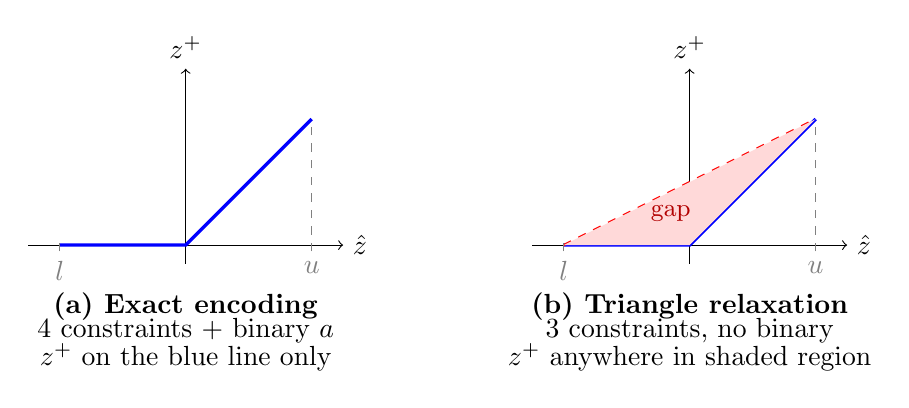
\begin{tikzpicture}[scale=0.8]
  % Left plot: exact ReLU
  \begin{scope}[shift={(-5,0)}]
    \draw[->] (-2.5,0) -- (2.5,0) node[right] {$\hat{z}$};
    \draw[->] (0,-0.3) -- (0,2.8) node[above] {$z^+$};
    % ReLU function
    \draw[very thick, blue] (-2,0) -- (0,0) -- (2,2);
    % Bounds
    \draw[dashed, gray] (-2,-0.1) node[below] {$l$} -- (-2,0.1);
    \draw[dashed, gray] (2,-0.1) node[below] {$u$} -- (2,2);
    \node[below] at (0,-0.6) {\textbf{(a) Exact encoding}};
    \node[below] at (0,-1.0) {4 constraints + binary $a$};
    \node[below] at (0,-1.4) {$z^+$ on the blue line only};
  \end{scope}
  % Right plot: triangle relaxation
  \begin{scope}[shift={(3,0)}]
    \draw[->] (-2.5,0) -- (2.5,0) node[right] {$\hat{z}$};
    \draw[->] (0,-0.3) -- (0,2.8) node[above] {$z^+$};
    % ReLU function
    \draw[very thick, blue] (-2,0) -- (0,0) -- (2,2);
    % Triangle upper envelope
    \draw[thick, red, dashed] (-2,0) -- (2,2);
    % Shaded triangle (the gap)
    \fill[red!15] (-2,0) -- (0,0) -- (2,2) -- (-2,0);
    % Gap area label
    \node[red!70!black] at (-0.3,0.5) {\small gap};
    % Bounds
    \draw[dashed, gray] (-2,-0.1) node[below] {$l$} -- (-2,0.1);
    \draw[dashed, gray] (2,-0.1) node[below] {$u$} -- (2,2);
    \node[below] at (0,-0.6) {\textbf{(b) Triangle relaxation}};
    \node[below] at (0,-1.0) {3 constraints, no binary};
    \node[below] at (0,-1.4) {$z^+$ anywhere in shaded region};
  \end{scope}
\end{tikzpicture}
\end{center}

\begin{itemize}[noitemsep]
  \item \textbf{Exact} (a): uses a binary variable $a \in \{0,1\}$ and
    4~constraints (Eqs.~(\ref{eq:bg_bigm1})--(\ref{eq:bg_bigm4})). $a=1$
    means ``neuron active, $z^+ = \hat z$''; $a=0$ means ``neuron
    inactive, $z^+ = 0$''. The post-ReLU value $z^+$ is forced onto the
    exact ReLU curve (blue line in diagram~(a)). This is precise but
    expensive: having to branch on $a$ is what makes verification
    NP-hard.
  \item \textbf{Relaxed} (b): drops the binary $a$ and uses 3~linear
    constraints (Eqs.~(\ref{eq:bg_tri1})--(\ref{eq:bg_tri3})). $z^+$ is
    now allowed to take any value inside the shaded triangle in
    diagram~(b). Every point on the true ReLU curve is still inside
    this triangle (so the relaxation \emph{over-covers} reality), but
    the triangle also admits some points that are not on the curve ---
    these extra admissible points are the price we pay. The shaded
    region between the blue line and the red dashed envelope is the
    \emph{gap}: the set of $(\hat z, z^+)$ pairs that the relaxation
    allows but the exact encoding would not.
\end{itemize}

The smaller the triangle, the less the relaxation loses. If $l$ is
very close to zero (the neuron ``wants'' to be active nearly always) or
$u$ is very close to zero (the neuron wants to be inactive nearly
always), the triangle is a thin sliver and the relaxation is almost
indistinguishable from the exact ReLU. Relaxing such a neuron costs
almost nothing and saves one binary. When $|l| \approx u$ the triangle
is fat --- the neuron is genuinely ambiguous and we do not want to
relax it.

\paragraph{Measuring ``almost decided'': the triangle's gap area.}
We quantify how thin the triangle is by its area. For a ReLU neuron
with pre-activation bounds $[l, u]$:
\begin{equation}
  \mathrm{gap}(l, u) \;=\;
    \begin{cases}
      0 & \text{if } l \ge 0 \text{ or } u \le 0
        \quad\text{(neuron is \emph{stable} --- not split at all)},\\[4pt]
      \displaystyle\frac{u \cdot |l|}{2\,(u - l)}
      & \text{otherwise (neuron is split; compute triangle area)}.
    \end{cases}
  \label{eq:gap_area}
\end{equation}
The second case is just the base-times-height formula for the triangle
in diagram~(b) (base $u - l$ along the $\hat z$-axis, peak offset
$u \cdot |l| / (u - l)$ above the ReLU line at $\hat z = 0$). Some
concrete numbers to build intuition:
\begin{center}
\footnotesize
\begin{tabular}{@{}c c c l@{}}
\toprule
$l$ & $u$ & $\mathrm{gap}(l, u)$ & Interpretation \\
\midrule
$-0.1$ & $2.0$  & $0.095$ & sliver: almost always active; cheap to relax \\
$-2.0$ & $0.1$  & $0.095$ & sliver: almost always inactive; cheap to relax \\
$-0.5$ & $0.5$  & $0.125$ & still fairly thin \\
$-1.0$ & $1.0$  & $0.25$  & moderate \\
$-2.0$ & $2.0$  & $0.5$   & big triangle; relaxation is noticeably loose \\
$-5.0$ & $5.0$  & $1.25$  & very fat; ambiguous neuron, leave exact \\
\bottomrule
\end{tabular}
\end{center}
A threshold $\tau$ drawn in the same units of (pre-activation area) lets
us say: ``relax any neuron whose triangle has area $\le \tau$, keep the
rest exact.'' Concretely:
\begin{itemize}[noitemsep]
  \item $\tau = 0.01$: relax only extremely thin slivers ($|l| < 0.02$
    or $u < 0.02$ in the table above).
  \item $\tau = 0.1$: relax most slivers but keep anything more than
    moderately split.
  \item $\tau = 0.5$: relax everything with gap $\le 0.5$, including
    the $[-2, 2]$ case above; genuinely ambiguous neurons (gap $> 0.5$)
    still keep their binary. This is aggressive but still below the
    fully-symmetric case.
  \item $\tau = 1.0$: relax almost every split neuron; fat triangles
    get replaced too. Strongest speedup, loosest answer.
  \item $\tau = \textsf{off}$: relax nothing --- every split neuron
    keeps its binary and its exact big-$M$ encoding.
\end{itemize}
So the ``$0.5$'' in \cli{adv\_std\_n2\_relax\_threshold=0.5} is
literally the maximum triangle-area any neuron can have and still be
converted from exact-with-binary to relaxed-without-binary.

\paragraph{Which binaries actually get dropped?}
Because VHAGaR encodes the network twice (see the next paragraph),
every split ReLU neuron $(m, k)$ owns \emph{two} binaries in the MIP:
$a^{\mathrm{org}}_{m,k}\!\in\!\{0,1\}$ on the clean-input copy and
$a^{\mathrm{pert}}_{m,k}\!\in\!\{0,1\}$ on the perturbed-input copy.
The relaxation decision is made per copy: for each copy
$c\in\{\mathrm{org},\mathrm{pert}\}$ whose gap
$g^{c}_{m,k}$ satisfies the tiered rule below, we remove
$a^{c}_{m,k}$ together with the two big-$M$ constraints that mention it
(Eqs.~(\ref{eq:bg_bigm3})--(\ref{eq:bg_bigm4})) and replace them with
the three triangle inequalities
(Eqs.~(\ref{eq:bg_tri1})--(\ref{eq:bg_tri3})) on that copy's interval
$[l^{N_2,c}_{m,k}, u^{N_2,c}_{m,k}]$. Concretely, three outcomes are
possible for a single neuron:
\begin{itemize}[noitemsep]
  \item drop \emph{both} $a^{\mathrm{org}}_{m,k}$ and
    $a^{\mathrm{pert}}_{m,k}$ (relax both copies);
  \item drop exactly one of them (relax only that copy; the other
    copy keeps its binary and its four big-$M$ constraints);
  \item keep both (no relaxation on this neuron).
\end{itemize}
Nothing else is touched in any of the three outcomes: the
pre-activations $\hat z^{\mathrm{org}}_{m,k}, \hat z^{\mathrm{pert}}_{m,k}$,
the post-ReLUs $z^{+,\mathrm{org}}_{m,k}, z^{+,\mathrm{pert}}_{m,k}$,
the neurons in adjacent layers, the inter-layer linear constraints,
and the perturbation-coupling constraints that link the two copies
all remain exactly as they were.

\paragraph{Why there are \emph{two} bounds per neuron (the org/pert twist).}
VHAGaR encodes each network twice inside one MIP: once for the clean
input $v_\mathrm{in}$ (the ``org'' copy) and once for the perturbed
input $v_{x_0} = v_\mathrm{in} + v_e$ (the ``pert'' copy). Every ReLU
neuron therefore has \emph{two} instances in the MIP: one on the org
copy with pre-activation bounds $[l^{N_2,\mathrm{org}}_{m,k},
u^{N_2,\mathrm{org}}_{m,k}]$, and one on the pert copy with (generally
looser, because the pert input box is wider) bounds
$[l^{N_2,\mathrm{pert}}_{m,k}, u^{N_2,\mathrm{pert}}_{m,k}]$. Each
instance has its own binary and its own triangle gap. This lets us
make the relaxation decision \emph{independently} per copy: we can
relax the org-copy binary, the pert-copy binary, both, or neither.

\paragraph{Decision rule (tiered, per-copy).}
Put everything together. For each ReLU neuron $(m, k)$ we compute
two gap numbers, one per copy:
\[
  g^{\mathrm{org}}_{m,k} =
    \mathrm{gap}\!\bigl(l^{N_2,\mathrm{org}}_{m,k},\,
                        u^{N_2,\mathrm{org}}_{m,k}\bigr),
  \qquad
  g^{\mathrm{pert}}_{m,k} =
    \mathrm{gap}\!\bigl(l^{N_2,\mathrm{pert}}_{m,k},\,
                        u^{N_2,\mathrm{pert}}_{m,k}\bigr),
\]
then compare each to the threshold $\tau$. There are three cases
(hence the word ``tiered''):
\begin{enumerate}[noitemsep]
  \item \textbf{Both tiny} --- if
    $\max(g^{\mathrm{org}}_{m,k}, g^{\mathrm{pert}}_{m,k})\le\tau$,
    both copies have thin triangles, so we drop \emph{both} binaries
    $a^{\mathrm{org}}_{m,k}$ and $a^{\mathrm{pert}}_{m,k}$ and put
    the triangle inequalities on both copies instead.
  \item \textbf{Only one tiny} --- if exactly one of the two gaps is
    $\le \tau$, we drop the binary for the smaller-gap copy only. The
    other copy keeps its binary and exact big-$M$ encoding. This is
    the case that motivates the name \tech{BoundTightPertRelax}: under
    a non-trivial perturbation the pert copy's bounds are looser (its
    triangle is bigger), so a neuron can easily be tight on the org
    side and still split on the pert side.
  \item \textbf{Neither tiny} --- if both gaps exceed $\tau$, the
    neuron is genuinely ambiguous on both sides. Keep the binary on
    both copies, do not relax.
\end{enumerate}
The per-copy bounds $l^{N_2,\mathrm{copy}}_{m,k},
u^{N_2,\mathrm{copy}}_{m,k}$ that feed $\mathrm{gap}(\cdot)$ are the
ones Bound Tightening already computed --- specifically, they are the
intersection of Source~A ($N_1$'s per-copy bound plus the diff) and
Source~B (the shared absolute-$N_2$ zonotope hull):
\begin{align}
  u^{N_2,\mathrm{copy}}_{m,k} &= \min\!\Bigl(
      \underbrace{u^{N_1,\mathrm{copy}}_{m,k} + d^{\uparrow}_{m,k}}_{\text{Source A: $N_1$ bound + diff}},\;
      \underbrace{u^{\mathrm{B}}_{m,k}}_{\text{Source B: $N_2$ zonotope hull}}
    \Bigr),
  \label{eq:btpr_upper_percopy}\\
  l^{N_2,\mathrm{copy}}_{m,k} &= \max\!\Bigl(
      l^{N_1,\mathrm{copy}}_{m,k} + d^{\downarrow}_{m,k},\;
      l^{\mathrm{B}}_{m,k}
    \Bigr).
  \label{eq:btpr_lower_percopy}
\end{align}
The org/pert asymmetry flows entirely through Source~A: $N_1$'s Phase-1
MIP is itself dual-copy, so its stored bound table
$\{(l^{N_1,\mathrm{copy}}_{m,k}, u^{N_1,\mathrm{copy}}_{m,k})\}$
distinguishes the two copies (the pert copy inherits a wider input
box $[-\ep, 1{+}\ep]^n$, so its bounds are typically looser). The
diff interval $[d^\downarrow_{m,k}, d^\uparrow_{m,k}]$ is shared
between copies. Source~B is also shared: its zonotope is initialised
to cover both input boxes at once, so a single hull is valid for
either copy. Therefore, the only reason $g^{\mathrm{org}}_{m,k}$ and
$g^{\mathrm{pert}}_{m,k}$ ever disagree is $N_1$'s own per-copy
bounds; when those happen to be identical at a neuron, both gaps
collapse to the same value and Tier~2 degenerates into Tier~1 or
Tier~3 there.

\paragraph{Safety net: the two copies are still linked.}
Even when we relax one copy and leave the other exact, the two are not
free to drift apart. VHAGaR's perturbed-interval coupling constraints
(always active in advstd safe combinations) link them via
$z^+_\mathrm{pert} - z^+_\mathrm{org} \in [\Delta^\downarrow,
\Delta^\uparrow]$, where $[\Delta^\downarrow, \Delta^\uparrow]$ is a
sound interval on how much the pert post-ReLU value can differ from
the org one under the perturbation budget. So relaxing a binary on one
side still indirectly constrains the other side.

\paragraph{Why $N_2$'s per-copy bounds (not $N_1$'s)?}
We judge a neuron's gap using $N_2$'s tightened bounds, not $N_1$'s,
for three reasons. (i)~The triangle constraints we emit use exactly
those $N_2$ bounds --- deciding on the same interval we later write
into the MIP is what makes the soundness argument work (see
``Consistency requirement'' and ``Soundness'' below). (ii)~Under
non-trivial perturbations, $N_2$'s org- and pert-copy bounds can
differ substantially (the pert copy sees a wider input box), so a
single-gap rule built on $N_1$ would miss the asymmetric
opportunities Tier~2 exploits. (iii)~The flag name itself ---
\tech{BoundTightPertRelax} --- advertises the dependency on
Bound Tightening's per-copy bound tightening.

\paragraph{Consistency requirement.}
The decision-time gaps $g^{\mathrm{org}}_{m,k}$ and
$g^{\mathrm{pert}}_{m,k}$ must be computed from the \emph{same}
intersected bounds that get baked into the emitted triangle
constraints. In the code, both sites call the shared helper
\texttt{intersect\_per\_copy\_bounds} in \texttt{core\_ops.jl}, so
there is no drift between ``the interval we decided was thin'' and
``the interval of the triangle we wrote into the MIP.'' This
invariant is what the soundness argument below rests on.

\paragraph{What does this cost, and what do we gain?}
Each neuron we relax removes one binary variable and two big-$M$
constraints from the MIP (and adds three linear inequalities), so on
a network with hundreds of split ReLUs we typically save dozens of
binaries. Since each binary in principle doubles Gurobi's
branch-and-bound tree, removing even a handful of binaries can cut
solve time substantially.

The price is that the reported $\delta$ is no longer guaranteed equal
to the exact optimum $\dexact$; it is now a \emph{sound upper bound}:
\[
  \delta_{\mathrm{relaxed}} \;\ge\; \dexact.
\]
In other words, if the relaxed MIP certifies robustness at some
$\delta$, then the exact MIP would also certify robustness at (at
worst) that same $\delta$. The overshoot grows with $\tau$, but since
we only relax neurons with gap $\le \tau$, each relaxation
contributes at most a small slice of looseness. In practice the
observed overshoot is often in the third decimal digit even at
$\tau = 0.5$.

\paragraph{Soundness.} Let $R\subseteq\{(m,k,\mathrm{copy})\}$ be the
set of (neuron, copy) pairs selected for relaxation by the tiered
rule, and let $\Fmip{2}^{(\{6\})}$ denote the feasible set of the
resulting N2 MIP. We claim
$\Fmip{2}\subseteq\Fmip{2}^{(\{6\})}$, hence
$\delta_{\mathrm{BTPR}}\ge\dexact$.
\begin{itemize}[noitemsep]
  \item For $(m,k,\mathrm{copy})\notin R$ the exact big-$M$ encoding is
    emitted, identical to the baseline; every $x\in\Fmip{2}$ trivially
    satisfies the same constraints.
  \item For $(m,k,\mathrm{copy})\in R$ the binary $a_{m,k,\mathrm{copy}}$
    and its four big-$M$ constraints are dropped; the three triangle
    inequalities are emitted on the \emph{same} per-copy bound
    $[l^{N_2,\mathrm{copy}}_{m,k},\,u^{N_2,\mathrm{copy}}_{m,k}]$ that
    would have gated the exact encoding (the consistency requirement
    above). By the triangle-relaxation lemma
    (Eqs.~(\ref{eq:bg_tri1})--(\ref{eq:bg_tri3})), every
    $(\hat{z},z^+)$ satisfying the exact ReLU encoding on
    $[l^{N_2,\mathrm{copy}}_{m,k},\,u^{N_2,\mathrm{copy}}_{m,k}]$ lies
    inside the triangle on the same interval. So every $x\in\Fmip{2}$
    satisfies the relaxed constraints.
\end{itemize}
All other constraints (perturbed-interval coupling, VHAGaR
dependencies, inter-layer linking, warmstart hints as non-constraining
hints) are unchanged. Therefore $\Fmip{2}\subseteq\Fmip{2}^{(\{6\})}$,
and taking the max of the unchanged objective over a superset can only
raise the value:
$\delta_{\mathrm{BTPR}}=\max_{x\in\Fmip{2}^{(\{6\})}}
\mathrm{obj}_{N_2}(x)\ge\max_{x\in\Fmip{2}}\mathrm{obj}_{N_2}(x)
=\dexact$.

\subsubsection{Algorithm and worked example}
\label{sec:tech3_alg}

\begin{algorithm}[H]
\caption{Per-Copy Triangle Drop on $N_2$ (\texttt{compute\_n2\_relax\_decision!})}
\label{alg:tech3}
\begin{algorithmic}[1]
\REQUIRE $N_2$ with dual encoding (org/pert copies), threshold $\tau$,
  per-copy $N_2$ bounds $(l^{N_2,c}_{m,k}, u^{N_2,c}_{m,k})$
  from Bound Tightening (Section~\ref{sec:bound_integration},
  eqs.~\ref{eq:btpr_upper_percopy}--\ref{eq:btpr_lower_percopy})
\STATE $\mathtt{n2\_relax\_decision} \leftarrow \{\}$
\FOR{each ReLU neuron $(m,k)$ in $N_2$}
  \STATE skip if stable on both copies
    \COMMENT{\texttt{relu()} short-circuits before the binary is allocated}
  \STATE $g^c \leftarrow \mathrm{gap}(l^{N_2,c}_{m,k},\, u^{N_2,c}_{m,k})$
    for $c \in \{\mathrm{org}, \mathrm{pert}\}$ (eq.~\ref{eq:gap_area})
  \IF{$\max(g^{\mathrm{org}}, g^{\mathrm{pert}}) \le \tau$}
    \STATE $(\mathrm{relax\_org}, \mathrm{relax\_pert}) \leftarrow (\textsf{true}, \textsf{true})$
      \COMMENT{both thin}
  \ELSIF{$\min(g^{\mathrm{org}}, g^{\mathrm{pert}}) \le \tau$}
    \STATE $(\mathrm{relax\_org}, \mathrm{relax\_pert}) \leftarrow$
      flag only $\arg\min_c g^c$
      \COMMENT{one thin}
  \ELSE
    \STATE $(\mathrm{relax\_org}, \mathrm{relax\_pert}) \leftarrow (\textsf{false}, \textsf{false})$
      \COMMENT{neither}
  \ENDIF
  \STATE record the joint flag pair under each pass's MIP key
    so \texttt{relu()} can dispatch on it at emission time
\ENDFOR
\STATE \textbf{During $\mathcal M_2$ build:} for each $(m, k, c)$ with
  flag $\textsf{true}$, drop binary $a^c_{m,k}$ and its two big-$M$
  rows (eqs.~\ref{eq:bg_bigm3}--\ref{eq:bg_bigm4}); emit the three
  triangle rows (eqs.~\ref{eq:bg_tri1}--\ref{eq:bg_tri3}) on
  $[l^{N_2,c}_{m,k}, u^{N_2,c}_{m,k}]$
\end{algorithmic}
\end{algorithm}

\paragraph{Variables / constraints per relaxed $(m,k,c)$.}
\emph{Removed:} 1 binary $a^c_{m,k}$ and 2 big-$M$ rows
(eqs.~\ref{eq:bg_bigm3}--\ref{eq:bg_bigm4}). \emph{Added:} 3 triangle
rows (eqs.~\ref{eq:bg_tri1}--\ref{eq:bg_tri3}) on the same
$\hat z^c_{m,k}, z^{+,c}_{m,k}$ variables. No new continuous variable.

\paragraph{Worked example.}
Same $N_1, N_2$ pair as Section~\ref{sec:tech1_alg}. Per-copy $N_2$
bounds for the hidden ReLU layer (taking Method-1 outputs and
extending the pert copy's $N_1$ bounds by the same diff):
\begin{center}\footnotesize
\begin{tabular}{l c c c}
\toprule
neuron & $(l, u)^{N_2,\mathrm{org}}$ & $(l, u)^{N_2,\mathrm{pert}}$ & $(g^{\mathrm{org}}, g^{\mathrm{pert}})$ \\
\midrule
$(1,1)$ & $(-0.3,\, 1.8)$ & $(-0.5,\, 2.0)$ & $(0.129,\, 0.200)$ \\
$(1,2)$ & $(-1.1,\, 0.9)$ & $(-1.3,\, 1.1)$ & $(0.248,\, 0.298)$ \\
\bottomrule
\end{tabular}\end{center}

\emph{Tier at $\tau = 0.15$.} Neuron $(1,1)$:
$g^{\mathrm{org}} = 0.129 \le 0.15 < g^{\mathrm{pert}}$, so
\emph{one-thin (org)} --- drop $a^{N_2,\mathrm{org}}_{1,1}$,
keep $a^{N_2,\mathrm{pert}}_{1,1}$. Neuron $(1,2)$: both gaps $>
0.15$, so \emph{neither-thin}.

\emph{Emitted on the relaxed org-copy of neuron $(1,1)$.}
Three rows (eqs.~\ref{eq:bg_tri1}--\ref{eq:bg_tri3}) on
$[l^{N_2,\mathrm{org}}_{1,1}, u^{N_2,\mathrm{org}}_{1,1}] =
[-0.3,\, 1.8]$:
\begin{align*}
  z^{+,\mathrm{org}}_{1,1} &\ge 0,\quad
  z^{+,\mathrm{org}}_{1,1} \ge \hat z^{\mathrm{org}}_{1,1},\quad
  z^{+,\mathrm{org}}_{1,1} \le
    \tfrac{1.8}{1.8 - (-0.3)}\bigl(\hat z^{\mathrm{org}}_{1,1} - (-0.3)\bigr)
    \approx 0.857\,(\hat z^{\mathrm{org}}_{1,1} + 0.3).
\end{align*}
The pert copy retains its four exact big-$M$ rows
(eqs.~\ref{eq:bg_bigm1}--\ref{eq:bg_bigm4}) and its binary
$a^{N_2,\mathrm{pert}}_{1,1}$. The two copies remain linked by the
perturbed-interval row (Section~\ref{sec:perturbed_intervals}'s
$z^{+,\mathrm{pert}}_{1,1} - z^{+,\mathrm{org}}_{1,1} \in [-0.2, 0.2]$),
which is what makes the one-thin tier sound.

\subsection{Sibling-Gated Refinement \textsf{(SibGate)}}
\label{sec:tech4}

\noindent
\textbf{Flag:} \cli{adv\_std\_n2\_sibling\_gate} $\in \{\textsf{false},\,
  \textsf{true}\}$.
\quad \textbf{Requires:} \cli{adv\_std\_n2\_relax\_threshold} (this technique
  augments Per-Copy Triangle Drop's tiered decision rule; it does not introduce one).
\quad \textbf{Model modification:} replaces the simple Wong--Kolter triangle
  with a conditional triangle gated on the surviving sibling binary in
  the ``one thin'' tier, and adds a pre-activation coupling constraint
  linking the two copies in the ``both thin'' tier.
\quad \textbf{Filename tag:} \texttt{\_SibGate} appended to the existing
  \texttt{\_BoundTightPertRelax\{$\tau$\}} tag.

\paragraph{What is changed.}
Per-Copy Triangle Drop's tiered per-copy decision rule (Section~\ref{sec:tech3}) is
inherited verbatim. Only the constraints emitted on each tier change:

\begin{center}
\footnotesize
\begin{tabular}{@{}l l l@{}}
\toprule
Tier & Per-Copy Triangle Drop (today) & Sibling-Gated Refinement (proposed) \\
\midrule
both thin & simple triangle on each copy &
  simple triangle on each copy \emph{plus} a single pre-activation
  coupling line linking them \\
one thin  & simple triangle on the relaxed copy &
  conditional triangle on the relaxed copy, gated on the kept sibling's
  binary, with intervals intersected against Bound Tightening's
  unconditional per-copy bound \\
neither   & exact big-$M$ on both & unchanged \\
\bottomrule
\end{tabular}
\end{center}

\subsubsection*{Tier ``one thin'' --- conditional triangle}

Let $c \in \{\mathrm{org}, \mathrm{pert}\}$ be the relaxed copy and
$\mathrm{pre}$ its sibling (the copy whose binary survives in the MIP):
$\mathrm{pre} = \mathrm{pert}$ when $c = \mathrm{org}$, and
$\mathrm{pre} = \mathrm{org}$ when $c = \mathrm{pert}$. Write
$a^{\mathrm{pre}}_{m,k}$ for the surviving sibling binary. Instead of
the three inequalities (\ref{eq:bg_tri1})--(\ref{eq:bg_tri3}) the MIP
receives four:
\begin{align}
  z^{c}_{m,k} &\ge 0, \quad
  z^{c}_{m,k} \ge \hat{z}^{c}_{m,k},
  \label{eq:tech4_lo}\\
  z^{c}_{m,k} &\le
    \tfrac{u_A}{u_A - l_A}\,(\hat{z}^{c}_{m,k} - l_A)
      + M\,(1 - a^{\mathrm{pre}}_{m,k}),
  \label{eq:tech4_hi_active}\\
  z^{c}_{m,k} &\le
    \tfrac{u_I}{u_I - l_I}\,(\hat{z}^{c}_{m,k} - l_I)
      + M\,a^{\mathrm{pre}}_{m,k},
  \label{eq:tech4_hi_inactive}
\end{align}
with $M = u^{N_2,c}_{m,k} + |l^{N_2,c}_{m,k}|$ chosen large enough to
make the ``off'' upper bound vacuous over the feasible region. (For
$c = \mathrm{org}$ this is exactly the conditional triangle of the
existing \cli{use\_relaxations} encoding; the $c = \mathrm{pert}$ case
is the symmetric mirror, gated on $a^{\mathrm{org}}_{m,k}$ instead.)

The four conditional bounds $l_A, u_A, l_I, u_I$ are built from
three sound interval inputs --- two of them produced by Bound Tightening
(\cli{adv\_std\_bound\_tightening}) and one of them produced by the
perturbation-coupling pipeline that backs \cli{use\_relaxations}:

\begin{itemize}[noitemsep]
  \item $[l^{N_2,c}_{m,k}, u^{N_2,c}_{m,k}]$ --- the unconditional
    pre-activation bound on the \emph{relaxed} copy $c$, produced by
    Bound Tightening's \texttt{intersect\_per\_copy\_bounds()} routine
    (Section~\ref{sec:bound_integration}).
  \item $[l^{N_2,\mathrm{pre}}_{m,k}, u^{N_2,\mathrm{pre}}_{m,k}]$ ---
    the same routine applied to the \emph{sibling} (kept-exact) copy
    $\mathrm{pre}$.
  \item $[l_{\mathrm{int}}, u_{\mathrm{int}}]$ --- the
    \emph{intended} input is a sound interval bound on the
    perturbation-induced pre-activation difference $\hat{z}^{c}_{m,k}
    - \hat{z}^{\mathrm{pre}}_{m,k}$ in $N_2$. The formula derivation
    in (\ref{eq:tech4_lAuA})--(\ref{eq:tech4_lIuI}) and the soundness
    proof below assume exactly that quantity, which is the
    pre-activation analogue of the post-activation coupling bound
    $[\Delta^\downarrow, \Delta^\uparrow]$ already used by the
    perturbed-interval constraints. \textbf{Caveat on today's code:}
    the routines that populate the global
    $\mathtt{relu\_comp\_*\_bounds}$ actually store
    $\hat z^{N_2,\mathrm{pert}} - \hat z^{N_1,\mathrm{org}}$, which
    bundles the org--pert perturbation diff with the $N_1$--$N_2$
    weight drift; the dispatch is gated on \cli{use\_relaxations} or
    \cli{adv\_std\_zono\_bounds}, \emph{not} on
    \cli{adv\_std\_bound\_tightening}, and the diff component (but not
    the pert component) becomes zonotope-tightened when
    \cli{adv\_std\_zono\_bounds}=true. The next paragraph spells out
    the recurrence the code uses and what changes are needed to
    expose the pure pert bound that this derivation needs.
\end{itemize}

\paragraph{How $[l_{\mathrm{int}}, u_{\mathrm{int}}]$ is computed in
the actual code.}
The quantity Sibling-Gated Refinement conceptually wants is the pre-activation
\emph{org--pert} diff $\hat z^{\mathrm{pert}}_{m,k} -
\hat z^{\mathrm{org}}_{m,k}$ in $N_2$. Inside both
$\mathtt{compute\_diff\_and\_comp\_bounds()}$ and its zonotope sibling
$\mathtt{compute\_diff\_bounds\_zonotope()}$
(\texttt{utils/perturbation\_intervals.jl}), this diff lives in two
4D arrays $\mathtt{pert\_up}, \mathtt{pert\_down}$. The recurrence
that propagates them through $N_2$ alone is verbatim:

\emph{Initialisation (input layer).}
$\mathtt{pert\_up} \leftarrow +\ep \cdot \mathbf{1}$,
$\mathtt{pert\_down} \leftarrow -\ep \cdot \mathbf{1}$.

\emph{Linear layer (with weights $W_2$).} Plain interval arithmetic;
the bias cancels in the difference:
\[
  \bigl[\mathtt{pert\_down}',\; \mathtt{pert\_up}'\bigr]
    \;=\; W_2 \cdot \bigl[\mathtt{pert\_down},\; \mathtt{pert\_up}\bigr].
\]

\emph{Conv layer (with filter $F_2$).} Same idea, via
$\mathtt{interval\_conv2d\_bounds}(F_2, F_2, \cdot)$ with zero bias.

\emph{ReLU layer.} Per-neuron clipping:
$\mathtt{pert\_up} \leftarrow \max(0,\, \mathtt{pert\_up})$,
$\mathtt{pert\_down} \leftarrow -\max(0,\, -\mathtt{pert\_down})$.

The two values stored at the input to each ReLU are then exactly the
quantity Sibling-Gated Refinement wants, and they would be the natural source for
$[l_{\mathrm{int},m,k}, u_{\mathrm{int},m,k}]$. The pert recurrence
is \emph{always interval arithmetic}, in both compute routines; the
zono flag does not switch it. (What the zono flag switches is the
\emph{diff} state that runs alongside, propagating
$\hat z^{N_2}_{m,k} - \hat z^{N_1}_{m,k}$ as a zonotope --- a separate
quantity.)

\paragraph{What the code actually exposes today
(\textsc{Important caveat}).}
At each ReLU layer the code does not push $\mathtt{pert\_up,
pert\_down}$ to a global. It only pushes the \emph{composed} bound
\[
  \mathtt{relu\_comp\_up}_{m,k}
    \;=\; \mathtt{diff\_up}_{m,k} + \mathtt{pert\_up}_{m,k},
  \qquad
  \mathtt{relu\_comp\_down}_{m,k}
    \;=\; \mathtt{diff\_down}_{m,k} + \mathtt{pert\_down}_{m,k},
\]
which bounds $\hat z^{N_2,\mathrm{pert}}_{m,k} -
\hat z^{N_1,\mathrm{org}}_{m,k}$ (weight drift \emph{and} input
perturbation combined). These are the
$\mathtt{relu\_comp\_*\_bounds}$ globals that today's
\cli{use\_relaxations} code reads. Two consequences:

\begin{enumerate}[noitemsep]
  \item If Sibling-Gated Refinement reads $\mathtt{relu\_comp\_*\_bounds}$ verbatim,
    its $[l_{\mathrm{int}}, u_{\mathrm{int}}]$ inherits the
    $N_1$--$N_2$ diff component on top of the org--pert perturbation
    --- that is \emph{not} what the conditional triangle's derivation
    in (\ref{eq:tech4_lAuA})--(\ref{eq:tech4_lIuI}) assumes, and the
    diff component does become zonotope-tightened when
    \cli{adv\_std\_zono\_bounds}=true.
  \item To match the derivation, the code change for Sibling-Gated Refinement needs
    to expose $\mathtt{pert\_up, pert\_down}$ at each ReLU as new
    globals (call them $\mathtt{relu\_pert\_*\_bounds}$) and have
    Sibling-Gated Refinement read those instead of $\mathtt{relu\_comp\_*}$. With
    that change, $[l_{\mathrm{int}}, u_{\mathrm{int}}]$ would always be
    interval, regardless of \cli{adv\_std\_zono\_bounds}, as the
    derivation requires.
\end{enumerate}

\paragraph{Flags that today trigger the routines (and what
\texttt{run\_relaxation\_sweep.py} sets).}
Both $\mathtt{compute\_diff\_and\_comp\_bounds()}$ and
$\mathtt{compute\_diff\_bounds\_zonotope()}$ are dispatched from
\texttt{utils/perturbation\_models.jl:486-497}. The dispatch fires
only when at least one of these flags is true:

\begin{itemize}[noitemsep]
  \item \cli{use\_relaxations}=true (with N1 binaries kept and N1
    encoded), \emph{or}
  \item \cli{adv\_std\_zono\_bounds}=true
    (\texttt{bound\_n2\_relu\_using\_zonotope}), \emph{or}
  \item one of the niche flags
    \texttt{bound\_n2\_xp\_using\_composed},
    \texttt{bound\_by\_zonotope\_n2\_hidden\_neurons\_which\_are\_not\_relu},
    \texttt{no\_n2\_xp\_encoding}, \texttt{no\_n1\_encoding\_at\_all},
    or $\mathtt{n1\_stability\_relax\_threshold} \ge 0$.
\end{itemize}
When the dispatch does fire, the choice between the two routines is
\cli{adv\_std\_zono\_bounds}: \texttt{false}~$\to$
$\mathtt{compute\_diff\_and\_comp\_bounds()}$, \texttt{true}~$\to$
$\mathtt{compute\_diff\_bounds\_zonotope()}$.

The Phase-2 invocation built by \texttt{run\_relaxation\_sweep.py}
(\texttt{run\_relaxation\_sweep.py:2486-2513}) does \emph{not} pass
\cli{use\_relaxations}, and Sibling-Gated Refinement's flag
\cli{adv\_std\_n2\_sibling\_gate} is not yet wired up. So in the sweep
the routines only fire on the rows where
\cli{adv\_std\_zono\_bounds}=true. Concretely:

\begin{itemize}[noitemsep]
  \item Sweep row with \cli{adv\_std\_zono\_bounds}=true:
    $\mathtt{relu\_comp\_*\_bounds}$ are populated by the zonotope
    variant. The diff side is zonotope-tightened, the pert side is
    interval --- so the comp bound is partially zonotope.
  \item Sweep row with \cli{adv\_std\_zono\_bounds}=false:
    $\mathtt{relu\_comp\_*\_bounds}$ are not populated at all. A
    Sibling-Gated Refinement emission that reads them would see empty arrays and
    have nothing to gate on; it would degrade to Per-Copy Triangle Drop.
\end{itemize}
The minimum code change to make Sibling-Gated Refinement active in the sweep is to
broaden the dispatch condition to also fire on
\cli{adv\_std\_n2\_sibling\_gate}=true, and to expose the pert state
as its own global so $[l_{\mathrm{int}}, u_{\mathrm{int}}]$ matches
the formula derivation rather than carrying weight drift on top.

With those inputs in hand, the conditional bounds are obtained by
intersecting Source-A-style conditional intervals (the first argument
of each $\max$/$\min$) with the unconditional per-copy bound on the
relaxed copy (the second argument):
\begin{align}
  l_A &\triangleq \max\!\bigl(l_{\mathrm{int}},\;
    l^{N_2,c}_{m,k}\bigr), &
  u_A &\triangleq \min\!\bigl(u^{N_2,\mathrm{pre}}_{m,k} + u_{\mathrm{int}},\;
    u^{N_2,c}_{m,k}\bigr),
  \label{eq:tech4_lAuA}\\
  l_I &\triangleq \max\!\bigl(l^{N_2,\mathrm{pre}}_{m,k} + l_{\mathrm{int}},\;
    l^{N_2,c}_{m,k}\bigr), &
  u_I &\triangleq \min\!\bigl(u_{\mathrm{int}},\;
    u^{N_2,c}_{m,k}\bigr).
  \label{eq:tech4_lIuI}
\end{align}
The first argument of each $\max$/$\min$ is what today's
\cli{use\_relaxations} code uses on its own (computed by
$\mathtt{compute\_diff\_and\_comp\_bounds()}$, currently gated on
\cli{use\_relaxations}, \emph{not} on \cli{adv\_std\_bound\_tightening}).
The second argument is the new contribution: the per-copy
unconditional bound $[l^{N_2,\cdot}_{m,k}, u^{N_2,\cdot}_{m,k}]$ that
Bound Tightening (\cli{adv\_std\_bound\_tightening}) produces via
$\mathtt{intersect\_per\_copy\_bounds()}$. So the conditional bounds
genuinely need \emph{both} pipelines to be active: the comp-bound
machinery to give the first argument, and Bound Tightening's per-copy
tightening to give the second. With either pipeline missing, the
intersection collapses to whichever side is still finite and
Sibling-Gated Refinement degrades --- in the limit, all the way back to
Per-Copy Triangle Drop.

\subsubsection*{Tier ``both thin'' --- pre-activation coupling}

Both binaries are dropped, both copies receive the simple triangle
exactly as in Per-Copy Triangle Drop. We additionally emit \emph{one} linear
constraint per neuron:
\begin{equation}
  l_{\mathrm{int}} \;\le\;
    \hat{z}^{\mathrm{pert}}_{m,k} - \hat{z}^{\mathrm{org}}_{m,k}
    \;\le\; u_{\mathrm{int}}.
  \label{eq:tech4_coupling}
\end{equation}
This constraint involves only existing pre-activation variables; no
binary, no big-$M$. Its purpose is to prevent the LP relaxation from
choosing the two copies' pre-activations independently. (At the
post-activation level the analogous coupling
$z^{+,\mathrm{pert}} - z^{+,\mathrm{org}} \in
[\Delta^\downarrow, \Delta^\uparrow]$ is already contributed by the
perturbed-interval coupling described after
Section~\ref{sec:bound_integration}; the new line is its missing
pre-activation analogue.)

\paragraph{Soundness --- ``one thin''.}
Let $\Fmip{2}$ be the feasible set of $N_2$'s exact MIP and let
$\Fmip{2}^{(4)}$ be the feasible set after Sibling-Gated Refinement emission. We
claim $\Fmip{2} \subseteq \Fmip{2}^{(4)}$.

Take any $x \in \Fmip{2}$ and any neuron $(m,k)$ in tier ``one thin'';
let $b = a^{\mathrm{pre}}_{m,k}(x) \in \{0,1\}$ be the realised value
of the kept sibling binary at $x$. We verify each of
(\ref{eq:tech4_lo})--(\ref{eq:tech4_hi_inactive}) at $x$.

The two lower bounds in (\ref{eq:tech4_lo}) appear in the exact ReLU
encoding too, so $x$ satisfies them.

For the upper bounds we split on $b$.

\emph{(i) $b = 1$.} The exact big-$M$ on the sibling enforces
$\hat z^{\mathrm{pre}}(x) \in [0, u^{N_2,\mathrm{pre}}_{m,k}]$.
Bound Tightening's diff bound gives
$\hat z^c(x) - \hat z^{\mathrm{pre}}(x) \in
[l_{\mathrm{int}}, u_{\mathrm{int}}]$, so
\[
  \hat z^c(x) \;\in\;
    \bigl[l_{\mathrm{int}},\;
      u^{N_2,\mathrm{pre}}_{m,k} + u_{\mathrm{int}}\bigr].
\]
Combining with Bound Tightening's unconditional bound
$\hat z^c(x) \in [l^{N_2,c}_{m,k}, u^{N_2,c}_{m,k}]$ and the definition
in (\ref{eq:tech4_lAuA}) yields $\hat z^c(x) \in [l_A, u_A]$. The
Wong--Kolter envelope on $[l_A, u_A]$ over-approximates
$\mathrm{ReLU}(\hat z)$ on that interval (the standard
triangle-relaxation lemma applied with endpoints $l_A, u_A$). Since
$z^c(x) = \mathrm{ReLU}(\hat z^c(x))$ under the exact encoding,
\[
  z^c(x) \;\le\;
    \tfrac{u_A}{u_A - l_A}\,(\hat z^c(x) - l_A),
\]
which together with $M(1 - b) = 0$ is exactly
(\ref{eq:tech4_hi_active}). Constraint
(\ref{eq:tech4_hi_inactive}) has slack $M \cdot b = M$ on its
right-hand side; by the choice of $M$ this is at least
$u^{N_2,c}_{m,k} \ge z^c(x)$, so the constraint is vacuous.

\emph{(ii) $b = 0$.} Symmetric: the exact big-$M$ on the sibling
enforces
$\hat z^{\mathrm{pre}}(x) \in [l^{N_2,\mathrm{pre}}_{m,k}, 0]$, hence
$\hat z^c(x) \in [l^{N_2,\mathrm{pre}}_{m,k} + l_{\mathrm{int}},\,
u_{\mathrm{int}}] \cap [l^{N_2,c}_{m,k}, u^{N_2,c}_{m,k}] =
[l_I, u_I]$ by (\ref{eq:tech4_lIuI}). The triangle envelope on
$[l_I, u_I]$ over-approximates $\mathrm{ReLU}$, giving
(\ref{eq:tech4_hi_inactive}) with $M \cdot b = 0$;
(\ref{eq:tech4_hi_active}) is vacuous by the same big-$M$ argument with
$M(1 - b) = M$.

So $x$ satisfies all four constraints, in either case of $b$.

\paragraph{Soundness --- ``both thin''.}
The added constraint (\ref{eq:tech4_coupling}) uses
$[l_{\mathrm{int}}, u_{\mathrm{int}}]$, which is derived by sound
interval-arithmetic propagation of the input perturbation through
$N_2$ in $\mathtt{compute\_diff\_and\_comp\_bounds()}$. Therefore for
every $x \in \Fmip{2}$, $\hat z^{\mathrm{pert}}(x) -
\hat z^{\mathrm{org}}(x) \in [l_{\mathrm{int}}, u_{\mathrm{int}}]$
holds by construction.

\paragraph{Why $\dexact$ remains in the search space.}
Combining the two soundness arguments above with the unchanged tier
``neither'' and the unchanged simple-triangle / big-$M$ encodings
everywhere else gives
\[
  \Fmip{2} \;\subseteq\; \Fmip{2}^{(4)}.
\]
Let $x^\ast \in \arg\max_{x \in \Fmip{2}} \mathrm{obj}_{N_2}(x)$, so by
definition $\mathrm{obj}_{N_2}(x^\ast) = \dexact$. Since
$x^\ast \in \Fmip{2} \subseteq \Fmip{2}^{(4)}$, the point $x^\ast$ is
also feasible under Sibling-Gated Refinement. The objective function is unchanged,
so
\[
  \delta_{\mathrm{SibGate}} \;\triangleq\;
    \max_{x \in \Fmip{2}^{(4)}} \mathrm{obj}_{N_2}(x)
    \;\ge\; \mathrm{obj}_{N_2}(x^\ast) \;=\; \dexact.
\]
Taking the max over a superset can only raise the value, so
$\dexact$ is in the SibGate search space and the reported
$\delta_{\mathrm{SibGate}}$ at \textsf{OPTIMAL} is a sound upper
bound on $\dexact$.

\paragraph{When the relaxation is genuinely tighter than Per-Copy Triangle Drop.}
The two conditional intervals
$[l_A, u_A], [l_I, u_I]$ are subintervals of $[l^{N_2,c}_{m,k},
u^{N_2,c}_{m,k}]$, so each conditional triangle is no fatter than the
single triangle Per-Copy Triangle Drop emits. The intersection step
(\ref{eq:tech4_lAuA})--(\ref{eq:tech4_lIuI}) shrinks them strictly
whenever Source~A's diff-derived bound and Source~B's absolute bound
disagree at a given endpoint (Theorem~\ref{thm:AB_incomparable}). The
``both thin'' coupling line shrinks the joint LP feasible region of
$(\hat z^{\mathrm{org}}, \hat z^{\mathrm{pert}})$ from a rectangle to a
slab. In each case the relaxation is at least as tight as Per-Copy Triangle Drop
and strictly tighter on neurons where the additional information binds.

\paragraph{Summary of SibGate's added constraints.}
On top of Per-Copy Triangle Drop's tiered emission, SibGate writes at most three
extra linear constraints per relaxed neuron --- and \emph{only} on
neurons that Per-Copy Triangle Drop already classified as ``thin enough'' for
some level of relaxation:
\begin{itemize}[noitemsep]
  \item \emph{Both-thin tier} (both binaries already dropped by
    Per-Copy Triangle Drop): SibGate adds the single
    pre-activation coupling line
    (\ref{eq:tech4_coupling}),
    $l_{\mathrm{int}} \le
      \hat z^{\mathrm{pert}}_{m,k} - \hat z^{\mathrm{org}}_{m,k}
      \le u_{\mathrm{int}}$.
    No binary, no big-$M$ --- just one slab tying the two preacts.
  \item \emph{One-thin tier} (binary dropped on copy $c$, kept on
    sibling $\mathrm{pre}$): SibGate \emph{replaces} the simple
    Wong--Kolter triangle on copy $c$ with the two big-$M$ conditional
    upper bounds (\ref{eq:tech4_hi_active})--(\ref{eq:tech4_hi_inactive}),
    each gated on the surviving sibling binary $a^{\mathrm{pre}}_{m,k}$.
    The two lower bounds (\ref{eq:tech4_lo}) are unchanged.
  \item \emph{Neither-thin tier}: SibGate touches nothing; Per-Copy Triangle Drop
    leaves both copies with their exact big-$M$ encoding.
\end{itemize}

\paragraph{Why \boldmath$\delta_{\mathrm{SibGate}} = \dexact$ at
\boldmath$\tau = 0$.}
At threshold $\tau = 0$ Per-Copy Triangle Drop's tiered rule collapses
significantly. Recall the gap formula (\ref{eq:gap_area}): for any
\emph{split} neuron ($l < 0 < u$) the triangle area
$\mathrm{gap}(l, u) > 0$ strictly; for any \emph{stable} neuron
($l \ge 0$ or $u \le 0$) it is exactly $0$. So the only way for a
gap to satisfy $g \le \tau = 0$ is for the neuron to be stable on
that copy. Walking the three tiers under this condition:
\begin{itemize}[noitemsep]
  \item \emph{Both-thin} requires $\max(g^{\mathrm{org}}, g^{\mathrm{pert}})
    \le 0$, i.e.\ both copies stable. But a neuron stable on both copies
    has no binary on either side (the big-$M$ encoding short-circuits
    on $l \ge 0$ or $u \le 0$ before ever allocating $a$), so the
    decision-precompute step
    (\texttt{compute\_n2\_relax\_decision!}, line~85 of
    \texttt{utils/n2\_relax\_decision.jl}) skips it via an early
    \texttt{continue}. \textbf{The both-thin tier is empty.}
  \item \emph{One-thin} requires $\min(g^{\mathrm{org}}, g^{\mathrm{pert}})
    \le 0$ with the other $> 0$. The relaxed copy $c$ is the stable
    side; the sibling is genuinely split and keeps its binary. But
    on the stable side \texttt{relu()} short-circuits at
    \texttt{core\_ops.jl:304/316} (returns $0$ for $u \le 0$ or $x$
    for $l \ge 0$) \emph{before} the Per-Copy Triangle Drop triangle path at
    line~562. No triangle is emitted on the stable copy --- and
    correspondingly \texttt{n2\_relu\_state[(\ldots, c)]} stays
    \texttt{nothing}. \texttt{apply\_sibgate\_constraints!} sees
    \texttt{st\_c === nothing} at line~64 and \texttt{continue}s
    without writing any constraint. \textbf{The one-thin tier emits
    nothing too.}
  \item \emph{Neither-thin} is the default for every genuinely split
    neuron (gap $> 0 > \tau$), and the standard exact big-$M$
    encoding is used.
\end{itemize}
Every neuron of the $N_2$ MIP therefore receives the exact big-$M$
encoding it would have received without any of Per-Copy Triangle Drop or
Sibling-Gated Refinement active. The bound globals SibGate populates
(\texttt{relu\_n2pert\_*\_bounds}, \texttt{n2\_preact\_*\_bounds} via
\texttt{compute\_n2\_pert\_relaxation\_bounds} at
\texttt{run.jl:971-973}) are consulted only by SibGate's own
post-encoding pass (which we just established is a no-op at $\tau=0$)
and by unrelated niche flags
(\cli{no\_n1\_binaries\_and\_relaxtions\_only\_on\_n2},
\cli{constrain\_n2\_xp\_via\_n1\_zonotope}); \texttt{intersect\_per\_copy\_bounds}
(Sources~A/B/C) never reads them. Consequently
\[
  \Fmip{2}^{(\textsf{SibGate}, \tau=0)} \;=\;
  \Fmip{2}^{(\tau=0)} \;=\; \Fmip{2},
\]
and at termination \textsf{OPTIMAL}
\[
  \delta_{\mathrm{SibGate}}\bigl|_{\tau=0} \;=\;
  \delta_{\mathrm{BTPR}}\bigl|_{\tau=0} \;=\; \dexact.
\]
Equality is \emph{constraint-level}: the same MIP is handed to Gurobi
in both modes. Reported wall-clock $t_\mathrm{adv}$ and the incumbent
returned at \texttt{TIME\_LIMIT} may still differ between the two
because Gurobi's parallel branch-and-bound is nondeterministic at the
default settings used here (\texttt{Threads}=32, \texttt{MIPFocus}=3,
no fixed \texttt{Seed}); two re-runs of either configuration alone
exhibit the same wallclock variance.

\subsubsection{Algorithm and worked example}
\label{sec:tech4_alg}

\begin{algorithm}[H]
\caption{Sibling-Gated Refinement on $N_2$}
\label{alg:tech4}
\begin{algorithmic}[1]
\REQUIRE $N_2$ with dual encoding, threshold $\tau$, per-copy bounds
  $(l^{N_2,c}_{m,k}, u^{N_2,c}_{m,k})$ from Bound Tightening, pre-act
  diff bound $(l_{\mathrm{int}}, u_{\mathrm{int}})_{m,k}$ propagated by
  the interval recurrence of Section~\ref{sec:perturbed_intervals} at
  the pre-ReLU site, tier assignment from Algorithm~\ref{alg:tech3}
\FOR{each ReLU neuron $(m,k)$ in $N_2$}
  \IF{tier is \emph{both thin}}
    \STATE keep the two simple triangles already emitted by
      Algorithm~\ref{alg:tech3} on each copy
    \STATE emit pre-act coupling row eq.~(\ref{eq:tech4_coupling}):\\
      $l_{\mathrm{int}} \le \hat z^{\mathrm{pert}}_{m,k} - \hat z^{\mathrm{org}}_{m,k} \le u_{\mathrm{int}}$
  \ELSIF{tier is \emph{one thin}, relaxed copy $c$, kept sibling $\mathrm{pre}$}
    \STATE compute $(l_A, u_A, l_I, u_I)$ via
      eqs.~(\ref{eq:tech4_lAuA})--(\ref{eq:tech4_lIuI})
    \STATE $M \leftarrow u^{N_2,c}_{m,k} + |l^{N_2,c}_{m,k}|$
    \STATE \emph{replace} the simple triangle on copy $c$ with the
      conditional triangle rows
      eqs.~(\ref{eq:tech4_lo})--(\ref{eq:tech4_hi_inactive}),
      each upper bound gated on existing sibling binary
      $a^{\mathrm{pre}}_{m,k}$
  \ELSE
    \STATE leave both copies with their exact big-$M$ encoding
  \ENDIF
\ENDFOR
\end{algorithmic}
\end{algorithm}

\paragraph{Variables / constraints added (per tier).}
\emph{Both thin:} 1 new row (pre-act coupling) on top of
Per-Copy Triangle Drop's 6 triangle rows; no new variable.
\emph{One thin:} 2 lower-bound rows
(eq.~\ref{eq:tech4_lo}) + 2 conditional upper-bound rows
(eqs.~\ref{eq:tech4_hi_active}--\ref{eq:tech4_hi_inactive}) on copy
$c$, each upper bound multiplied by the existing sibling binary
$a^{\mathrm{pre}}_{m,k}$ via a big-$M$ slack; no new variable.
\emph{Neither thin:} unchanged.

\paragraph{Worked example (one-thin tier).}
Same $N_2$ pair and bounds as Section~\ref{sec:tech3_alg}. At
$\tau = 0.15$, neuron $(1,1)$ is one-thin with $c = \mathrm{org}$,
$\mathrm{pre} = \mathrm{pert}$.

\emph{Pre-act diff bound at neuron $(1,1)$.} Using the
\emph{interval}-arithmetic recurrence of
Section~\ref{sec:perturbed_intervals} at the pre-ReLU site
(``How $[l_{\mathrm{int}}, u_{\mathrm{int}}]$ is computed in the
actual code'' paragraph): $(l_{\mathrm{int}}, u_{\mathrm{int}}) =
(-0.2,\, +0.2)$.

\emph{Apply eqs.~(\ref{eq:tech4_lAuA})--(\ref{eq:tech4_lIuI}).}
\begin{align*}
  l_A &= \max(l_{\mathrm{int}},\, l^{N_2,\mathrm{org}}_{1,1})
       = \max(-0.2,\, -0.3) = -0.2 \\
  u_A &= \min(u^{N_2,\mathrm{pert}}_{1,1} + u_{\mathrm{int}},\,
              u^{N_2,\mathrm{org}}_{1,1})
       = \min(2.0 + 0.2,\, 1.8) = 1.8 \\
  l_I &= \max(l^{N_2,\mathrm{pert}}_{1,1} + l_{\mathrm{int}},\,
              l^{N_2,\mathrm{org}}_{1,1})
       = \max(-0.5 + (-0.2),\, -0.3) = -0.3 \\
  u_I &= \min(u_{\mathrm{int}},\, u^{N_2,\mathrm{org}}_{1,1})
       = \min(0.2,\, 1.8) = 0.2 \\
  M   &= u^{N_2,\mathrm{org}}_{1,1} + |l^{N_2,\mathrm{org}}_{1,1}| = 2.1.
\end{align*}

\emph{Emitted on the relaxed org-copy.} The two lower bounds
(eq.~\ref{eq:tech4_lo}) plus the two conditional uppers
(eqs.~\ref{eq:tech4_hi_active}--\ref{eq:tech4_hi_inactive}):
\begin{align*}
  z^{\mathrm{org}}_{1,1} &\ge 0,\quad z^{\mathrm{org}}_{1,1} \ge \hat z^{\mathrm{org}}_{1,1}, \\
  z^{\mathrm{org}}_{1,1} &\le \tfrac{1.8}{1.8-(-0.2)}(\hat z^{\mathrm{org}}_{1,1} - (-0.2))
    + 2.1\,(1 - a^{\mathrm{pert}}_{1,1})
    = 0.9\,(\hat z^{\mathrm{org}}_{1,1} + 0.2) + 2.1\,(1 - a^{\mathrm{pert}}_{1,1}), \\
  z^{\mathrm{org}}_{1,1} &\le \tfrac{0.2}{0.2-(-0.3)}(\hat z^{\mathrm{org}}_{1,1} - (-0.3))
    + 2.1\,a^{\mathrm{pert}}_{1,1}
    = 0.4\,(\hat z^{\mathrm{org}}_{1,1} + 0.3) + 2.1\,a^{\mathrm{pert}}_{1,1}.
\end{align*}
When $a^{\mathrm{pert}}_{1,1} = 1$ the second row is active and the
third is slack; vice versa for $a^{\mathrm{pert}}_{1,1} = 0$. On the
active branch SibGate's envelope is over $[-0.2, 1.8]$ (vs the
unconditional $[-0.3, 1.8]$ from Per-Copy Triangle Drop); on the
inactive branch it is over $[-0.3, 0.2]$ (vs $[-0.3, 1.8]$).

\paragraph{Worked example (both-thin tier).}
At $\tau = 0.5$ neuron $(1,1)$ enters the both-thin tier (both gaps
$\le 0.5$). Per-Copy Triangle Drop now emits two simple triangles,
one on each copy ($[-0.3, 1.8]$ and $[-0.5, 2.0]$). SibGate
\emph{additionally} emits the coupling row
\[
  -0.2 \;\le\; \hat z^{\mathrm{pert}}_{1,1} - \hat z^{\mathrm{org}}_{1,1} \;\le\; +0.2
\]
on the existing pre-activation variables, with no binary and no
big-$M$. This forbids the LP relaxation from choosing the two
pre-acts independently --- a constraint the perturbed-interval
post-act coupling already enforces post-ReLU but not pre-ReLU
(Section~\ref{sec:pi_required}, item~(iii)).

\section{Safe-to-Use Combinations}
\label{sec:safe}

% BEGIN AUTO: safe_tables
Tables below list \emph{every} recorded advstd combination at all seeds, all $\tau$ values, evaluated per-architecture and broken out by perturbation type and size. Each row corresponds to a single $(c_\mathrm{src}, c_\mathrm{tgt})$ cell of one combo (rows for the same combo are grouped, with the flag columns shown only on the first cell of the combo). We report wall-clock \textsf{t\_std} and \textsf{t\_adv} per cell, the per-cell speedup \textsf{sp}$=\textsf{t\_std}/\textsf{t\_adv}$ (higher is better; $>\!1$ means advstd finished faster than the with-perturbed-intervals baseline), $\overline{\text{sp}}_{c\_\mathrm{src}}$ (mean \textsf{sp} over all tested $c_\mathrm{tgt}$ for the same $c_\mathrm{src}$ within a combo, shown once per $c_\mathrm{src}$ group), and \textsf{n\_relax} (per-cell number of N2 binary variables removed by Technique~3). The \tech{bound\_tight} column labels which Technique~1 variant is used (\texttt{interval} / \texttt{zono} / \texttt{none}; \tech{n1Probe} is always off), and the $\tau$ column is the Technique~3 threshold. Within each (perturbation, size) block combos are sorted by descending mean \textsf{sp} (fastest advstd first); cells within a combo are sorted by $(c_\mathrm{src}, c_\mathrm{tgt})$. \tech{mipStart} and \tech{lpBasis} are always off and omitted for brevity. Cells where both modes hit Gurobi's \texttt{TIME\_LIMIT} are shown with their wall-clock times; for those cells, a separate per-arch gap-comparison table reports how often advstd reached a tighter $u - l$ bound on the objective than standard, alongside the mean gap of each method.

\noindent\textbf{Note:} every table below --- the overall combination ranking, the per-arch perturbation tables, and the per-arch \texttt{TIME\_LIMIT} gap-comparison tables --- is restricted to the 4 combinations \texttt{zono:prev\_pgd:0.0+sg}, \texttt{zono:prev\_pgd:0.5+sg}, \texttt{interval:prev\_pgd:0.0+sg}, \texttt{interval:prev\_pgd:0.5+sg} (via \texttt{--combination\_table}).

% auto-generated: archs=[cnn1=92combos/1579cells(timeout-combos=64), 3x50=42combos/763cells(timeout-combos=75), 3x10=88combos/1389cells(timeout-combos=0)], seed=None, tau=None, combo_filter=zono:prev_pgd:0.0+sg,zono:prev_pgd:0.5+sg,interval:prev_pgd:0.0+sg,interval:prev_pgd:0.5+sg
\begin{table}[!htbp]
\centering
\scriptsize
\setlength{\tabcolsep}{5pt}
\begin{adjustbox}{max width=\textwidth,center}%
\begin{tabular}{@{}r l l l | r r r r >{\raggedright\arraybackslash}p{3.2cm} >{\raggedright\arraybackslash}p{6.2cm}@{}}
\hline
\# & \tech{bound\_tight} & \tech{varHint} & $\tau$ & $\overline{\text{sp}}$ & n\_wins & n\_cells & win\_rate & $\langle$arch, pert, p\_size$\rangle$ where standard beats advstd on every $c_\mathrm{src}$ & $\langle$arch, $c_\mathrm{src}\rangle$ where, on \emph{every} tested (pert, p\_size), advstd was either faster on average ($\overline{\text{sp}}>1$), or both methods averaged at the wall-clock cap ($\overline{t_\mathrm{std}}\!\approx\!\overline{t_\mathrm{adv}}\!\approx\!T$, so the $\overline{\text{sp}}\!\le\!1$ verdict is a timeout artefact) AND advstd's $u\!-\!l$ gap on the timeout cells was no worse than standard's (entries needing this timeout-tied clause for at least one (pert, p\_size) are tagged \textit{(tied at TIME\_LIMIT)}) \\
\hline
\rowcolor{blue!12}   1 & interval    & prev\_pgd & 0.5+sg & \textbf{1.380} &   251 &    386 & \textbf{65.03\%} & \textit{none} & \texttt{<3x10,\discretionary{}{}{}2>}\textsuperscript{*}; \texttt{<3x10,\discretionary{}{}{}1>}; \texttt{<cnn1,\discretionary{}{}{}0>}; \texttt{<{3x50,\discretionary{}{}{}cnn1},\discretionary{}{}{}1>}~\textit{(tied at TIME\_LIMIT)}; \texttt{<3x50,\discretionary{}{}{}0>}~\textit{(tied at TIME\_LIMIT)} \\
\hline
\rowcolor{blue!12}   2 & zono        & prev\_pgd & 0.5+sg & \textbf{1.335} &   299 &    460 & \textbf{65.00\%} & \textit{none} & \texttt{<cnn1,\discretionary{}{}{}2>}\textsuperscript{*}; \texttt{<3x50,\discretionary{}{}{}1>}~\textit{(tied at TIME\_LIMIT)}; \texttt{<3x50,\discretionary{}{}{}0>}~\textit{(tied at TIME\_LIMIT)} \\
\hline
\rowcolor{blue!12}   3 & zono        & prev\_pgd & 0.0+sg & \textbf{1.273} &   292 &    463 & \textbf{63.07\%} & \textit{none} & \texttt{<3x10,\discretionary{}{}{}1>}; \texttt{<cnn1,\discretionary{}{}{}0>}; \texttt{<3x50,\discretionary{}{}{}0>}~\textit{(tied at TIME\_LIMIT)} \\
\hline
\rowcolor{blue!12}   4 & interval    & prev\_pgd & 0.0+sg & \textbf{1.337} &   240 &    391 & \textbf{61.38\%} & \textit{none} & \texttt{<3x10,\discretionary{}{}{}1>}; \texttt{<3x10,\discretionary{}{}{}2>}\textsuperscript{*}; \texttt{<{3x50,\discretionary{}{}{}cnn1},\discretionary{}{}{}1>}~\textit{(tied at TIME\_LIMIT)}; \texttt{<3x50,\discretionary{}{}{}0>}~\textit{(tied at TIME\_LIMIT)} \\
\hline
\end{tabular}%
\end{adjustbox}
\caption{Overall advstd combination ranking at all seeds, all $\tau$ values --- one row per flag combination, aggregated over every (arch, pert, size, $c_\mathrm{src}$, $c_\mathrm{tgt}$) cell in the per-arch tables below. $\overline{\text{sp}}$: mean per-cell $\text{sp}=\textsf{t\_std}/\textsf{t\_adv}$; \textsf{n\_wins} counts cells with $\text{sp}>1$; \textsf{win\_rate}=\textsf{n\_wins}/\textsf{n\_cells} (bold when $>\!50\%$). \textsf{losers}: $\langle$arch, pert, p\_size$\rangle$ triples where every tested $c_\mathrm{src}$ averaged $\text{sp}<1$. \textsf{winners}: $\langle$arch, $c_\mathrm{src}\rangle$ pairs where every tested (pert, p\_size) averaged $\text{sp}>1$, or $\overline{t_\mathrm{std}}$ and $\overline{t_\mathrm{adv}}$ both sat within 60\,s of the observed \texttt{TIME\_LIMIT} cap \emph{and} the gap rule ($\overline{\text{gap}}_\mathrm{adv}\le\overline{\text{gap}}_\mathrm{std}$ or $|\overline{\text{gap}}_\mathrm{std}-\overline{\text{gap}}_\mathrm{adv}|<0.05$) holds on the timeout cells (such entries are tagged \textit{(tied at TIME\_LIMIT)}); \textsuperscript{*} flags partial coverage (some (pert, p\_size) for this arch were not exercised by this combo). Sorted by descending \textsf{win\_rate}, then $\overline{\text{sp}}$; $\overline{\text{sp}}>1$ in \textbf{bold}. Rows are shaded blue.}
\label{tab:safe_overall_combo_ranking}
\end{table}
\clearpage
\section*{Per-perturbation histograms: $\overline{\text{sp}}$ paired with win-rate}
The figures below answer ``which advstd combination should I pick on this perturbation $\times$ architecture?'' from \emph{two} angles at once. Each row of paired charts shows a single $\langle\text{arch}, \text{pert}\rangle$ slice twice: the \textbf{left} chart reports the combo's mean speed-up (how fast it is on average), the \textbf{right} chart reports its win rate (how often it actually beats standard). Combos occupy a \textbf{stable x position} across both charts of a row \emph{and} across every row of an arch (alphabetical on the combo abbreviation), so a reader can scan one column down the page and watch a combo's behaviour change as the perturbation type changes in either metric.\par\medskip \noindent\textbf{Left chart} --- bar height $=$ the arithmetic mean of $\overline{\text{sp}}$ across every $c_\mathrm{src}\times c_\mathrm{tgt}\times$ seed cell across all p\_sizes of the perturbation type. \textbf{Each bar is vertically split} into a \emph{solid bottom} and a \emph{faded $+$ diagonally hatched top} in the same combo colour: the solid fraction equals $\textsf{wins}/\textsf{p\_sizes}$, where a p\_size's \textsf{win} is defined by a \emph{hybrid} rule that mirrors the orange gap-comparison table's treatment of the two cell populations --- a p\_size in which every cell finished (no \texttt{TIME\_LIMIT}) wins iff $\overline{\text{sp}}>1$; a p\_size in which every cell hit \texttt{TIME\_LIMIT} wins iff $\overline{\text{gap}}_\mathrm{adv}<\overline{\text{gap}}_\mathrm{std}$ across its timeout cells; a p\_size with cells of both kinds is judged \emph{per cell} and wins iff a majority of cells win on their own type (each non-timeout cell votes \emph{yes} when $\text{sp}>1$, each timeout cell votes \emph{yes} when its $u-l$ gap on advstd is tighter than on standard). Bars above $3.0$ are clipped at that height and the true value is printed in \textbf{bold} above the bar; the dashed line marks the $\overline{\text{sp}}=1$ breakeven.\par\medskip \noindent\textbf{Right chart} --- each column encodes three quantities by nested rectangles on an absolute-count $y$-axis (scale $0\to n_{\max}$, where $n_{\max}$ is the largest \textsf{n\_cells} of any combo on the chart, marked by a dashed reference line): a faint \emph{envelope} of height $n_{\max}$ (maximum coverage anywhere on the chart); a mid-grey \emph{tests} rectangle of height \textsf{n\_cells} (this combo's actual coverage on the slice); and a coloured \emph{wins} bar inside, split into a \emph{solid bottom} $=$ $\textsf{finished wins}$ (cells where the run finished and advstd was faster, $\text{sp}>1$) and a \emph{faded $+$ hatched top} $=$ $\textsf{timeout wins}$ (cells where both modes hit \texttt{TIME\_LIMIT} and advstd's $\overline{\text{gap}}_\mathrm{adv}<\overline{\text{gap}}_\mathrm{std}$). The combo's \textbf{win rate} is therefore the fraction of the mid-grey rectangle that is coloured; an under-tested combo's column is visibly shorter than its envelope. A combo with no timeout cells shows a fully solid coloured bar, and a combo whose wins all came from tighter-gap timeout cells shows only a hatched top.\par\medskip \noindent The \textcolor{orange!85!black}{$\bigstar$} above each chart marks the best combo on that chart (highest $\overline{\text{sp}}$ on the left, highest win rate on the right --- the two stars may pick different combos when the orderings disagree). A best-to-worst ranking summary line sits above each chart with the per-combo metric value and the relevant breakdown ($\textsf{wins}/\textsf{p\_sizes}$ for sp, $(\textsf{finished}+\textsf{timeout})/\textsf{n}$ for win rate). Cells with mismatched \texttt{--timout} caps between the two modes are excluded (same rule as the per-arch perturbation tables and the blue overall ranking).

\noindent\textbf{Note:} these histograms are restricted to the 4 combinations \texttt{zono:prev\_pgd:0.0+sg}, \texttt{zono:prev\_pgd:0.5+sg}, \texttt{interval:prev\_pgd:0.0+sg}, \texttt{interval:prev\_pgd:0.5+sg} (via \texttt{--combination\_table}).

% auto-generated: 12 paired sp+win-rate rows across 3 archs, seed=None, tau=None, combo_filter=zono:prev_pgd:0.0+sg,zono:prev_pgd:0.5+sg,interval:prev_pgd:0.0+sg,interval:prev_pgd:0.5+sg


\clearpage
\subsection*{Architecture \textbf{cnn1} --- $\overline{\text{sp}}$ paired with win-rate}
\label{tab:perthist_cnn1}
This page shows 4 paired rows, one per \textbf{perturbation type} measured on \textbf{cnn1}. Each row repeats the same $\langle\text{arch}, \text{pert}\rangle$ slice twice: the \emph{left} chart is the mean-speedup view (section intro above); the \emph{right} chart is the win-rate view (same intro, different bar definition). Combo columns occupy the same x position in both charts of a row, so a column can be scanned down the page to follow one combo across perturbation types in both metrics.
\par\medskip\noindent
\begin{minipage}[t]{0.48\linewidth}
\begin{center}
\scriptsize
\colorbox{yellow!40}{\textbf{sp}}\;\textbf{cnn1} \textbar{} pert \textbf{patch} (p\_sizes merged: \texttt{1,14,14,3}) \textbar{} 4 combos, total $n=90$ cells.\\[0.4ex]
\textbf{Ranking (best $\to$ worst):}\ \textcolor{orange!85!black}{$\bigstar$}\textcolor{orange!80!black}{\rule{0.55em}{0.55em}}\,2.13\,(1/1) ~ \textcolor{red!75!black}{\rule{0.55em}{0.55em}}\,1.88\,(1/1) ~ \textcolor{green!55!black}{\rule{0.55em}{0.55em}}\,1.66\,(1/1) ~ \textcolor{blue!75!black}{\rule{0.55em}{0.55em}}\,1.41\,(1/1)\\[0.4ex]
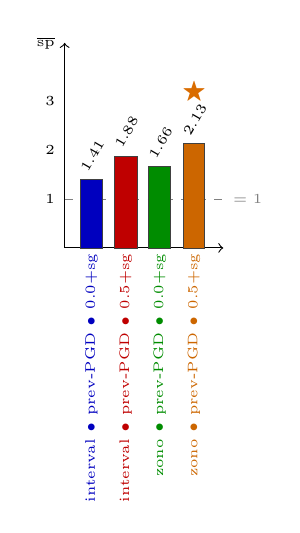
\begin{tikzpicture}[scale=0.62, every node/.style={font=\tiny}]
  \draw[->] (0,0) -- (3.25,0);
  \draw[->] (0,0) -- (0,4.20) node[left]{$\overline{\text{sp}}$};
  \draw[dashed, gray] (0,1) -- (3.25,1) node[right]{$=1$};
  \node[left, font=\tiny] at (0,1) {1};
  \node[left, font=\tiny] at (0,2) {2};
  \node[left, font=\tiny] at (0,3) {3};
  \fill[blue!75!black] (0.33,0) rectangle (0.78,1.409);
  \draw[gray!50!black, line width=0.2pt] (0.33,0) rectangle (0.78,1.409);
  \node[anchor=south west, rotate=60, font=\tiny, inner sep=1pt] at (0.50,1.459) {1.41};
  \node[anchor=east, rotate=90, font=\tiny, text=blue!75!black, inner sep=1pt] at (0.55,-0.05) {interval $\bullet$ prev-PGD $\bullet$ 0.0+sg};
  \fill[red!75!black] (1.02,0) rectangle (1.48,1.884);
  \draw[gray!50!black, line width=0.2pt] (1.02,0) rectangle (1.48,1.884);
  \node[anchor=south west, rotate=60, font=\tiny, inner sep=1pt] at (1.20,1.934) {1.88};
  \node[anchor=east, rotate=90, font=\tiny, text=red!75!black, inner sep=1pt] at (1.25,-0.05) {interval $\bullet$ prev-PGD $\bullet$ 0.5+sg};
  \fill[green!55!black] (1.72,0) rectangle (2.17,1.664);
  \draw[gray!50!black, line width=0.2pt] (1.72,0) rectangle (2.17,1.664);
  \node[anchor=south west, rotate=60, font=\tiny, inner sep=1pt] at (1.90,1.714) {1.66};
  \node[anchor=east, rotate=90, font=\tiny, text=green!55!black, inner sep=1pt] at (1.95,-0.05) {zono $\bullet$ prev-PGD $\bullet$ 0.0+sg};
  \fill[orange!80!black] (2.42,0) rectangle (2.87,2.134);
  \draw[gray!50!black, line width=0.2pt] (2.42,0) rectangle (2.87,2.134);
  \node[anchor=south west, rotate=60, font=\tiny, inner sep=1pt] at (2.60,2.184) {2.13};
  \node[anchor=east, rotate=90, font=\tiny, text=orange!80!black, inner sep=1pt] at (2.65,-0.05) {zono $\bullet$ prev-PGD $\bullet$ 0.5+sg};
  \node[font=\small, text=orange!85!black] at (2.65,3.18) {$\bigstar$};
\end{tikzpicture}
\end{center}
\end{minipage}
\hfill
\begin{minipage}[t]{0.48\linewidth}
\begin{center}
\scriptsize
\colorbox{cyan!30}{\textbf{win}}\;\textbf{cnn1} \textbar{} pert \textbf{patch} (p\_sizes merged: \texttt{1,14,14,3}) \textbar{} 4 combos, total $n=90$ cells, $n_{\max}=27$.\\[0.4ex]
\textbf{Ranking (best $\to$ worst):}\ \textcolor{orange!85!black}{$\bigstar$}\textcolor{red!75!black}{\rule{0.55em}{0.55em}}\,89\%\,(16f+0t/18) ~ \textcolor{orange!80!black}{\rule{0.55em}{0.55em}}\,89\%\,(24f+0t/27) ~ \textcolor{blue!75!black}{\rule{0.55em}{0.55em}}\,72\%\,(13f+0t/18) ~ \textcolor{green!55!black}{\rule{0.55em}{0.55em}}\,67\%\,(18f+0t/27)\\[0.4ex]
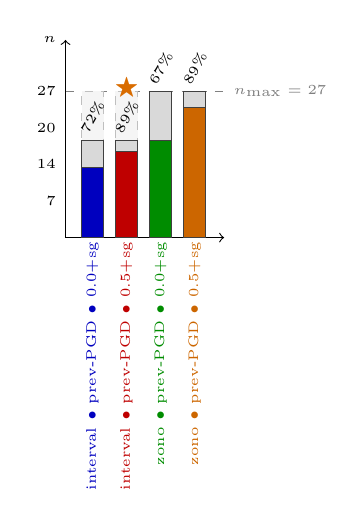
\begin{tikzpicture}[scale=0.62, every node/.style={font=\tiny}]
  \draw[->] (0,0) -- (3.25,0);
  \draw[->] (0,0) -- (0,4.05) node[left]{$n$};
  \draw[dashed, gray] (0,3.00) -- (3.25,3.00) node[right]{$n_{\max}=27$};
  \node[left, font=\tiny] at (0,0.75) {7};
  \node[left, font=\tiny] at (0,1.50) {14};
  \node[left, font=\tiny] at (0,2.25) {20};
  \node[left, font=\tiny] at (0,3.00) {27};
  \fill[gray!8] (0.33,0) rectangle (0.78,3.000);
  \draw[gray!50, line width=0.2pt, dashed] (0.33,0) rectangle (0.78,3.000);
  \fill[gray!30] (0.33,0) rectangle (0.78,2.000);
  \draw[gray!50!black, line width=0.2pt] (0.33,0) rectangle (0.78,2.000);
  \fill[blue!75!black] (0.33,0) rectangle (0.78,1.444);
  \draw[gray!50!black, line width=0.2pt] (0.33,0) rectangle (0.78,1.444);
  \node[anchor=south west, rotate=60, font=\tiny, inner sep=1pt] at (0.50,2.020) {72\%};
  \node[anchor=east, rotate=90, font=\tiny, text=blue!75!black, inner sep=1pt] at (0.55,-0.02) {interval $\bullet$ prev-PGD $\bullet$ 0.0+sg};
  \fill[gray!8] (1.02,0) rectangle (1.48,3.000);
  \draw[gray!50, line width=0.2pt, dashed] (1.02,0) rectangle (1.48,3.000);
  \fill[gray!30] (1.02,0) rectangle (1.48,2.000);
  \draw[gray!50!black, line width=0.2pt] (1.02,0) rectangle (1.48,2.000);
  \fill[red!75!black] (1.02,0) rectangle (1.48,1.778);
  \draw[gray!50!black, line width=0.2pt] (1.02,0) rectangle (1.48,1.778);
  \node[anchor=south west, rotate=60, font=\tiny, inner sep=1pt] at (1.20,2.020) {89\%};
  \node[anchor=east, rotate=90, font=\tiny, text=red!75!black, inner sep=1pt] at (1.25,-0.02) {interval $\bullet$ prev-PGD $\bullet$ 0.5+sg};
  \fill[gray!8] (1.72,0) rectangle (2.17,3.000);
  \draw[gray!50, line width=0.2pt, dashed] (1.72,0) rectangle (2.17,3.000);
  \fill[gray!30] (1.72,0) rectangle (2.17,3.000);
  \draw[gray!50!black, line width=0.2pt] (1.72,0) rectangle (2.17,3.000);
  \fill[green!55!black] (1.72,0) rectangle (2.17,2.000);
  \draw[gray!50!black, line width=0.2pt] (1.72,0) rectangle (2.17,2.000);
  \node[anchor=south west, rotate=60, font=\tiny, inner sep=1pt] at (1.90,3.020) {67\%};
  \node[anchor=east, rotate=90, font=\tiny, text=green!55!black, inner sep=1pt] at (1.95,-0.02) {zono $\bullet$ prev-PGD $\bullet$ 0.0+sg};
  \fill[gray!8] (2.42,0) rectangle (2.87,3.000);
  \draw[gray!50, line width=0.2pt, dashed] (2.42,0) rectangle (2.87,3.000);
  \fill[gray!30] (2.42,0) rectangle (2.87,3.000);
  \draw[gray!50!black, line width=0.2pt] (2.42,0) rectangle (2.87,3.000);
  \fill[orange!80!black] (2.42,0) rectangle (2.87,2.667);
  \draw[gray!50!black, line width=0.2pt] (2.42,0) rectangle (2.87,2.667);
  \node[anchor=south west, rotate=60, font=\tiny, inner sep=1pt] at (2.60,3.020) {89\%};
  \node[anchor=east, rotate=90, font=\tiny, text=orange!80!black, inner sep=1pt] at (2.65,-0.02) {zono $\bullet$ prev-PGD $\bullet$ 0.5+sg};
  \node[font=\small, text=orange!85!black] at (1.25,3.05) {$\bigstar$};
\end{tikzpicture}
\end{center}
\end{minipage}

\par\medskip\noindent
\begin{minipage}[t]{0.48\linewidth}
\begin{center}
\scriptsize
\colorbox{yellow!40}{\textbf{sp}}\;\textbf{cnn1} \textbar{} pert \textbf{occ} (p\_sizes merged: \texttt{3,3,5}, \texttt{5,5,5}) \textbar{} 4 combos, total $n=153$ cells.\\[0.4ex]
\textbf{Ranking (best $\to$ worst):}\ \textcolor{orange!85!black}{$\bigstar$}\textcolor{blue!75!black}{\rule{0.55em}{0.55em}}\,2.05\,(2/2) ~ \textcolor{red!75!black}{\rule{0.55em}{0.55em}}\,2.03\,(2/2) ~ \textcolor{orange!80!black}{\rule{0.55em}{0.55em}}\,1.79\,(2/2) ~ \textcolor{green!55!black}{\rule{0.55em}{0.55em}}\,1.78\,(2/2)\\[0.4ex]
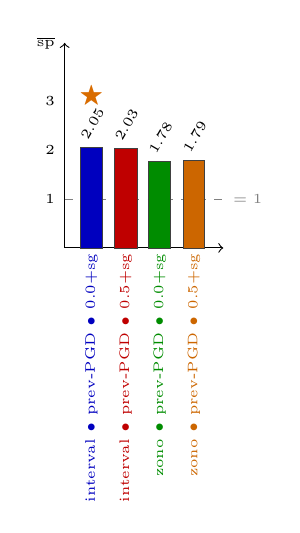
\begin{tikzpicture}[scale=0.62, every node/.style={font=\tiny}]
  \draw[->] (0,0) -- (3.25,0);
  \draw[->] (0,0) -- (0,4.20) node[left]{$\overline{\text{sp}}$};
  \draw[dashed, gray] (0,1) -- (3.25,1) node[right]{$=1$};
  \node[left, font=\tiny] at (0,1) {1};
  \node[left, font=\tiny] at (0,2) {2};
  \node[left, font=\tiny] at (0,3) {3};
  \fill[blue!75!black] (0.33,0) rectangle (0.78,2.053);
  \draw[gray!50!black, line width=0.2pt] (0.33,0) rectangle (0.78,2.053);
  \node[anchor=south west, rotate=60, font=\tiny, inner sep=1pt] at (0.50,2.103) {2.05};
  \node[anchor=east, rotate=90, font=\tiny, text=blue!75!black, inner sep=1pt] at (0.55,-0.05) {interval $\bullet$ prev-PGD $\bullet$ 0.0+sg};
  \fill[red!75!black] (1.02,0) rectangle (1.48,2.032);
  \draw[gray!50!black, line width=0.2pt] (1.02,0) rectangle (1.48,2.032);
  \node[anchor=south west, rotate=60, font=\tiny, inner sep=1pt] at (1.20,2.082) {2.03};
  \node[anchor=east, rotate=90, font=\tiny, text=red!75!black, inner sep=1pt] at (1.25,-0.05) {interval $\bullet$ prev-PGD $\bullet$ 0.5+sg};
  \fill[green!55!black] (1.72,0) rectangle (2.17,1.778);
  \draw[gray!50!black, line width=0.2pt] (1.72,0) rectangle (2.17,1.778);
  \node[anchor=south west, rotate=60, font=\tiny, inner sep=1pt] at (1.90,1.828) {1.78};
  \node[anchor=east, rotate=90, font=\tiny, text=green!55!black, inner sep=1pt] at (1.95,-0.05) {zono $\bullet$ prev-PGD $\bullet$ 0.0+sg};
  \fill[orange!80!black] (2.42,0) rectangle (2.87,1.790);
  \draw[gray!50!black, line width=0.2pt] (2.42,0) rectangle (2.87,1.790);
  \node[anchor=south west, rotate=60, font=\tiny, inner sep=1pt] at (2.60,1.840) {1.79};
  \node[anchor=east, rotate=90, font=\tiny, text=orange!80!black, inner sep=1pt] at (2.65,-0.05) {zono $\bullet$ prev-PGD $\bullet$ 0.5+sg};
  \node[font=\small, text=orange!85!black] at (0.55,3.10) {$\bigstar$};
\end{tikzpicture}
\end{center}
\end{minipage}
\hfill
\begin{minipage}[t]{0.48\linewidth}
\begin{center}
\scriptsize
\colorbox{cyan!30}{\textbf{win}}\;\textbf{cnn1} \textbar{} pert \textbf{occ} (p\_sizes merged: \texttt{3,3,5}, \texttt{5,5,5}) \textbar{} 4 combos, total $n=153$ cells, $n_{\max}=45$.\\[0.4ex]
\textbf{Ranking (best $\to$ worst):}\ \textcolor{orange!85!black}{$\bigstar$}\textcolor{red!75!black}{\rule{0.55em}{0.55em}}\,64\%\,(23f+0t/36) ~ \textcolor{orange!80!black}{\rule{0.55em}{0.55em}}\,64\%\,(23f+0t/36) ~ \textcolor{green!55!black}{\rule{0.55em}{0.55em}}\,58\%\,(26f+0t/45) ~ \textcolor{blue!75!black}{\rule{0.55em}{0.55em}}\,56\%\,(20f+0t/36)\\[0.4ex]
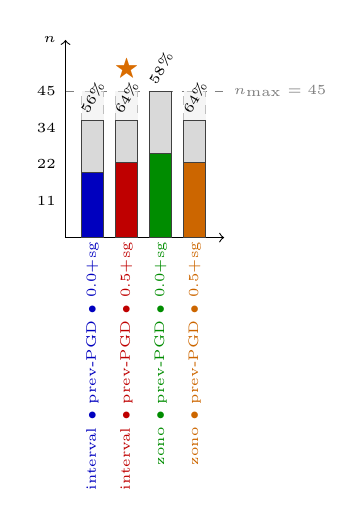
\begin{tikzpicture}[scale=0.62, every node/.style={font=\tiny}]
  \draw[->] (0,0) -- (3.25,0);
  \draw[->] (0,0) -- (0,4.05) node[left]{$n$};
  \draw[dashed, gray] (0,3.00) -- (3.25,3.00) node[right]{$n_{\max}=45$};
  \node[left, font=\tiny] at (0,0.75) {11};
  \node[left, font=\tiny] at (0,1.50) {22};
  \node[left, font=\tiny] at (0,2.25) {34};
  \node[left, font=\tiny] at (0,3.00) {45};
  \fill[gray!8] (0.33,0) rectangle (0.78,3.000);
  \draw[gray!50, line width=0.2pt, dashed] (0.33,0) rectangle (0.78,3.000);
  \fill[gray!30] (0.33,0) rectangle (0.78,2.400);
  \draw[gray!50!black, line width=0.2pt] (0.33,0) rectangle (0.78,2.400);
  \fill[blue!75!black] (0.33,0) rectangle (0.78,1.333);
  \draw[gray!50!black, line width=0.2pt] (0.33,0) rectangle (0.78,1.333);
  \node[anchor=south west, rotate=60, font=\tiny, inner sep=1pt] at (0.50,2.420) {56\%};
  \node[anchor=east, rotate=90, font=\tiny, text=blue!75!black, inner sep=1pt] at (0.55,-0.02) {interval $\bullet$ prev-PGD $\bullet$ 0.0+sg};
  \fill[gray!8] (1.02,0) rectangle (1.48,3.000);
  \draw[gray!50, line width=0.2pt, dashed] (1.02,0) rectangle (1.48,3.000);
  \fill[gray!30] (1.02,0) rectangle (1.48,2.400);
  \draw[gray!50!black, line width=0.2pt] (1.02,0) rectangle (1.48,2.400);
  \fill[red!75!black] (1.02,0) rectangle (1.48,1.533);
  \draw[gray!50!black, line width=0.2pt] (1.02,0) rectangle (1.48,1.533);
  \node[anchor=south west, rotate=60, font=\tiny, inner sep=1pt] at (1.20,2.420) {64\%};
  \node[anchor=east, rotate=90, font=\tiny, text=red!75!black, inner sep=1pt] at (1.25,-0.02) {interval $\bullet$ prev-PGD $\bullet$ 0.5+sg};
  \fill[gray!8] (1.72,0) rectangle (2.17,3.000);
  \draw[gray!50, line width=0.2pt, dashed] (1.72,0) rectangle (2.17,3.000);
  \fill[gray!30] (1.72,0) rectangle (2.17,3.000);
  \draw[gray!50!black, line width=0.2pt] (1.72,0) rectangle (2.17,3.000);
  \fill[green!55!black] (1.72,0) rectangle (2.17,1.733);
  \draw[gray!50!black, line width=0.2pt] (1.72,0) rectangle (2.17,1.733);
  \node[anchor=south west, rotate=60, font=\tiny, inner sep=1pt] at (1.90,3.020) {58\%};
  \node[anchor=east, rotate=90, font=\tiny, text=green!55!black, inner sep=1pt] at (1.95,-0.02) {zono $\bullet$ prev-PGD $\bullet$ 0.0+sg};
  \fill[gray!8] (2.42,0) rectangle (2.87,3.000);
  \draw[gray!50, line width=0.2pt, dashed] (2.42,0) rectangle (2.87,3.000);
  \fill[gray!30] (2.42,0) rectangle (2.87,2.400);
  \draw[gray!50!black, line width=0.2pt] (2.42,0) rectangle (2.87,2.400);
  \fill[orange!80!black] (2.42,0) rectangle (2.87,1.533);
  \draw[gray!50!black, line width=0.2pt] (2.42,0) rectangle (2.87,1.533);
  \node[anchor=south west, rotate=60, font=\tiny, inner sep=1pt] at (2.60,2.420) {64\%};
  \node[anchor=east, rotate=90, font=\tiny, text=orange!80!black, inner sep=1pt] at (2.65,-0.02) {zono $\bullet$ prev-PGD $\bullet$ 0.5+sg};
  \node[font=\small, text=orange!85!black] at (1.25,3.45) {$\bigstar$};
\end{tikzpicture}
\end{center}
\end{minipage}

\par\medskip\noindent
\begin{minipage}[t]{0.48\linewidth}
\begin{center}
\scriptsize
\colorbox{yellow!40}{\textbf{sp}}\;\textbf{cnn1} \textbar{} pert \textbf{translation} (p\_sizes merged: \texttt{1,1}, \texttt{3,1}, \texttt{3,3}) \textbar{} 4 combos, total $n=231$ cells.\\[0.4ex]
\textbf{Ranking (best $\to$ worst):}\ \textcolor{orange!85!black}{$\bigstar$}\textcolor{red!75!black}{\rule{0.55em}{0.55em}}\,1.45\,(3/3) ~ \textcolor{blue!75!black}{\rule{0.55em}{0.55em}}\,1.43\,(3/3) ~ \textcolor{orange!80!black}{\rule{0.55em}{0.55em}}\,1.39\,(3/3) ~ \textcolor{green!55!black}{\rule{0.55em}{0.55em}}\,1.28\,(3/3)\\[0.4ex]
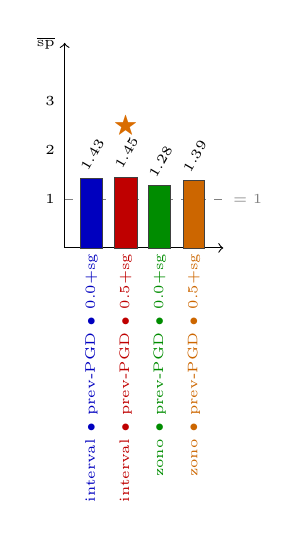
\begin{tikzpicture}[scale=0.62, every node/.style={font=\tiny}]
  \draw[->] (0,0) -- (3.25,0);
  \draw[->] (0,0) -- (0,4.20) node[left]{$\overline{\text{sp}}$};
  \draw[dashed, gray] (0,1) -- (3.25,1) node[right]{$=1$};
  \node[left, font=\tiny] at (0,1) {1};
  \node[left, font=\tiny] at (0,2) {2};
  \node[left, font=\tiny] at (0,3) {3};
  \fill[blue!75!black] (0.33,0) rectangle (0.78,1.427);
  \draw[gray!50!black, line width=0.2pt] (0.33,0) rectangle (0.78,1.427);
  \node[anchor=south west, rotate=60, font=\tiny, inner sep=1pt] at (0.50,1.477) {1.43};
  \node[anchor=east, rotate=90, font=\tiny, text=blue!75!black, inner sep=1pt] at (0.55,-0.05) {interval $\bullet$ prev-PGD $\bullet$ 0.0+sg};
  \fill[red!75!black] (1.02,0) rectangle (1.48,1.454);
  \draw[gray!50!black, line width=0.2pt] (1.02,0) rectangle (1.48,1.454);
  \node[anchor=south west, rotate=60, font=\tiny, inner sep=1pt] at (1.20,1.504) {1.45};
  \node[anchor=east, rotate=90, font=\tiny, text=red!75!black, inner sep=1pt] at (1.25,-0.05) {interval $\bullet$ prev-PGD $\bullet$ 0.5+sg};
  \fill[green!55!black] (1.72,0) rectangle (2.17,1.284);
  \draw[gray!50!black, line width=0.2pt] (1.72,0) rectangle (2.17,1.284);
  \node[anchor=south west, rotate=60, font=\tiny, inner sep=1pt] at (1.90,1.334) {1.28};
  \node[anchor=east, rotate=90, font=\tiny, text=green!55!black, inner sep=1pt] at (1.95,-0.05) {zono $\bullet$ prev-PGD $\bullet$ 0.0+sg};
  \fill[orange!80!black] (2.42,0) rectangle (2.87,1.392);
  \draw[gray!50!black, line width=0.2pt] (2.42,0) rectangle (2.87,1.392);
  \node[anchor=south west, rotate=60, font=\tiny, inner sep=1pt] at (2.60,1.442) {1.39};
  \node[anchor=east, rotate=90, font=\tiny, text=orange!80!black, inner sep=1pt] at (2.65,-0.05) {zono $\bullet$ prev-PGD $\bullet$ 0.5+sg};
  \node[font=\small, text=orange!85!black] at (1.25,2.50) {$\bigstar$};
\end{tikzpicture}
\end{center}
\end{minipage}
\hfill
\begin{minipage}[t]{0.48\linewidth}
\begin{center}
\scriptsize
\colorbox{cyan!30}{\textbf{win}}\;\textbf{cnn1} \textbar{} pert \textbf{translation} (p\_sizes merged: \texttt{1,1}, \texttt{3,1}, \texttt{3,3}) \textbar{} 4 combos, total $n=231$ cells, $n_{\max}=67$.\\[0.4ex]
\textbf{Ranking (best $\to$ worst):}\ \textcolor{orange!85!black}{$\bigstar$}\textcolor{red!75!black}{\rule{0.55em}{0.55em}}\,74\%\,(31f+6t/50) ~ \textcolor{orange!80!black}{\rule{0.55em}{0.55em}}\,70\%\,(40f+7t/67) ~ \textcolor{blue!75!black}{\rule{0.55em}{0.55em}}\,70\%\,(29f+6t/50) ~ \textcolor{green!55!black}{\rule{0.55em}{0.55em}}\,61\%\,(32f+7t/64)\\[0.4ex]
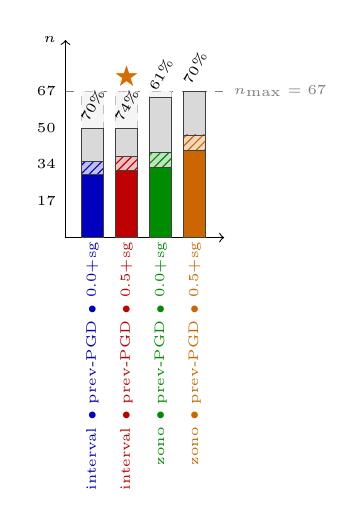
\begin{tikzpicture}[scale=0.62, every node/.style={font=\tiny}]
  \draw[->] (0,0) -- (3.25,0);
  \draw[->] (0,0) -- (0,4.05) node[left]{$n$};
  \draw[dashed, gray] (0,3.00) -- (3.25,3.00) node[right]{$n_{\max}=67$};
  \node[left, font=\tiny] at (0,0.75) {17};
  \node[left, font=\tiny] at (0,1.50) {34};
  \node[left, font=\tiny] at (0,2.25) {50};
  \node[left, font=\tiny] at (0,3.00) {67};
  \fill[gray!8] (0.33,0) rectangle (0.78,3.000);
  \draw[gray!50, line width=0.2pt, dashed] (0.33,0) rectangle (0.78,3.000);
  \fill[gray!30] (0.33,0) rectangle (0.78,2.239);
  \draw[gray!50!black, line width=0.2pt] (0.33,0) rectangle (0.78,2.239);
  \fill[blue!75!black] (0.33,0) rectangle (0.78,1.299);
  \draw[gray!50!black, line width=0.2pt] (0.33,0) rectangle (0.78,1.299);
  \fill[white] (0.33,1.299) rectangle (0.78,1.567);
  \fill[blue!75!black, opacity=0.25] (0.33,1.299) rectangle (0.78,1.567);
  \fill[pattern=north east lines, pattern color=blue!75!black] (0.33,1.299) rectangle (0.78,1.567);
  \draw[gray!50!black, line width=0.2pt] (0.33,1.299) rectangle (0.78,1.567);
  \node[anchor=south west, rotate=60, font=\tiny, inner sep=1pt] at (0.50,2.259) {70\%};
  \node[anchor=east, rotate=90, font=\tiny, text=blue!75!black, inner sep=1pt] at (0.55,-0.02) {interval $\bullet$ prev-PGD $\bullet$ 0.0+sg};
  \fill[gray!8] (1.02,0) rectangle (1.48,3.000);
  \draw[gray!50, line width=0.2pt, dashed] (1.02,0) rectangle (1.48,3.000);
  \fill[gray!30] (1.02,0) rectangle (1.48,2.239);
  \draw[gray!50!black, line width=0.2pt] (1.02,0) rectangle (1.48,2.239);
  \fill[red!75!black] (1.02,0) rectangle (1.48,1.388);
  \draw[gray!50!black, line width=0.2pt] (1.02,0) rectangle (1.48,1.388);
  \fill[white] (1.02,1.388) rectangle (1.48,1.657);
  \fill[red!75!black, opacity=0.25] (1.02,1.388) rectangle (1.48,1.657);
  \fill[pattern=north east lines, pattern color=red!75!black] (1.02,1.388) rectangle (1.48,1.657);
  \draw[gray!50!black, line width=0.2pt] (1.02,1.388) rectangle (1.48,1.657);
  \node[anchor=south west, rotate=60, font=\tiny, inner sep=1pt] at (1.20,2.259) {74\%};
  \node[anchor=east, rotate=90, font=\tiny, text=red!75!black, inner sep=1pt] at (1.25,-0.02) {interval $\bullet$ prev-PGD $\bullet$ 0.5+sg};
  \fill[gray!8] (1.72,0) rectangle (2.17,3.000);
  \draw[gray!50, line width=0.2pt, dashed] (1.72,0) rectangle (2.17,3.000);
  \fill[gray!30] (1.72,0) rectangle (2.17,2.866);
  \draw[gray!50!black, line width=0.2pt] (1.72,0) rectangle (2.17,2.866);
  \fill[green!55!black] (1.72,0) rectangle (2.17,1.433);
  \draw[gray!50!black, line width=0.2pt] (1.72,0) rectangle (2.17,1.433);
  \fill[white] (1.72,1.433) rectangle (2.17,1.746);
  \fill[green!55!black, opacity=0.25] (1.72,1.433) rectangle (2.17,1.746);
  \fill[pattern=north east lines, pattern color=green!55!black] (1.72,1.433) rectangle (2.17,1.746);
  \draw[gray!50!black, line width=0.2pt] (1.72,1.433) rectangle (2.17,1.746);
  \node[anchor=south west, rotate=60, font=\tiny, inner sep=1pt] at (1.90,2.886) {61\%};
  \node[anchor=east, rotate=90, font=\tiny, text=green!55!black, inner sep=1pt] at (1.95,-0.02) {zono $\bullet$ prev-PGD $\bullet$ 0.0+sg};
  \fill[gray!8] (2.42,0) rectangle (2.87,3.000);
  \draw[gray!50, line width=0.2pt, dashed] (2.42,0) rectangle (2.87,3.000);
  \fill[gray!30] (2.42,0) rectangle (2.87,3.000);
  \draw[gray!50!black, line width=0.2pt] (2.42,0) rectangle (2.87,3.000);
  \fill[orange!80!black] (2.42,0) rectangle (2.87,1.791);
  \draw[gray!50!black, line width=0.2pt] (2.42,0) rectangle (2.87,1.791);
  \fill[white] (2.42,1.791) rectangle (2.87,2.104);
  \fill[orange!80!black, opacity=0.25] (2.42,1.791) rectangle (2.87,2.104);
  \fill[pattern=north east lines, pattern color=orange!80!black] (2.42,1.791) rectangle (2.87,2.104);
  \draw[gray!50!black, line width=0.2pt] (2.42,1.791) rectangle (2.87,2.104);
  \node[anchor=south west, rotate=60, font=\tiny, inner sep=1pt] at (2.60,3.020) {70\%};
  \node[anchor=east, rotate=90, font=\tiny, text=orange!80!black, inner sep=1pt] at (2.65,-0.02) {zono $\bullet$ prev-PGD $\bullet$ 0.5+sg};
  \node[font=\small, text=orange!85!black] at (1.25,3.29) {$\bigstar$};
\end{tikzpicture}
\end{center}
\end{minipage}

\par\medskip\noindent
\begin{minipage}[t]{0.48\linewidth}
\begin{center}
\scriptsize
\colorbox{yellow!40}{\textbf{sp}}\;\textbf{cnn1} \textbar{} pert \textbf{linf} (p\_sizes merged: \texttt{0.1}) \textbar{} 4 combos, total $n=57$ cells.\\[0.4ex]
\textbf{Ranking (best $\to$ worst):}\ \textcolor{orange!85!black}{$\bigstar$}\textcolor{green!55!black}{\rule{0.55em}{0.55em}}\,1.00\,(1/1) ~ \textcolor{orange!80!black}{\rule{0.55em}{0.55em}}\,1.00\,(1/1) ~ \textcolor{blue!75!black}{\rule{0.55em}{0.55em}}\,1.00\,(1/1) ~ \textcolor{red!75!black}{\rule{0.55em}{0.55em}}\,1.00\,(1/1)\\[0.4ex]
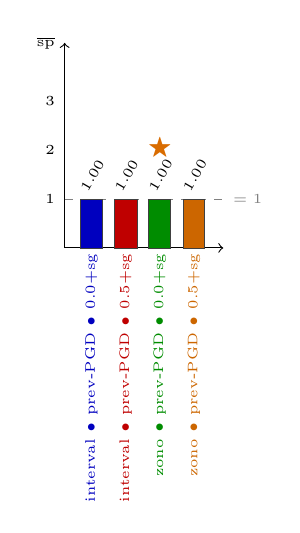
\begin{tikzpicture}[scale=0.62, every node/.style={font=\tiny}]
  \draw[->] (0,0) -- (3.25,0);
  \draw[->] (0,0) -- (0,4.20) node[left]{$\overline{\text{sp}}$};
  \draw[dashed, gray] (0,1) -- (3.25,1) node[right]{$=1$};
  \node[left, font=\tiny] at (0,1) {1};
  \node[left, font=\tiny] at (0,2) {2};
  \node[left, font=\tiny] at (0,3) {3};
  \fill[blue!75!black] (0.33,0) rectangle (0.78,1.000);
  \draw[gray!50!black, line width=0.2pt] (0.33,0) rectangle (0.78,1.000);
  \node[anchor=south west, rotate=60, font=\tiny, inner sep=1pt] at (0.50,1.050) {1.00};
  \node[anchor=east, rotate=90, font=\tiny, text=blue!75!black, inner sep=1pt] at (0.55,-0.05) {interval $\bullet$ prev-PGD $\bullet$ 0.0+sg};
  \fill[red!75!black] (1.02,0) rectangle (1.48,1.000);
  \draw[gray!50!black, line width=0.2pt] (1.02,0) rectangle (1.48,1.000);
  \node[anchor=south west, rotate=60, font=\tiny, inner sep=1pt] at (1.20,1.050) {1.00};
  \node[anchor=east, rotate=90, font=\tiny, text=red!75!black, inner sep=1pt] at (1.25,-0.05) {interval $\bullet$ prev-PGD $\bullet$ 0.5+sg};
  \fill[green!55!black] (1.72,0) rectangle (2.17,1.001);
  \draw[gray!50!black, line width=0.2pt] (1.72,0) rectangle (2.17,1.001);
  \node[anchor=south west, rotate=60, font=\tiny, inner sep=1pt] at (1.90,1.051) {1.00};
  \node[anchor=east, rotate=90, font=\tiny, text=green!55!black, inner sep=1pt] at (1.95,-0.05) {zono $\bullet$ prev-PGD $\bullet$ 0.0+sg};
  \fill[orange!80!black] (2.42,0) rectangle (2.87,1.001);
  \draw[gray!50!black, line width=0.2pt] (2.42,0) rectangle (2.87,1.001);
  \node[anchor=south west, rotate=60, font=\tiny, inner sep=1pt] at (2.60,1.051) {1.00};
  \node[anchor=east, rotate=90, font=\tiny, text=orange!80!black, inner sep=1pt] at (2.65,-0.05) {zono $\bullet$ prev-PGD $\bullet$ 0.5+sg};
  \node[font=\small, text=orange!85!black] at (1.95,2.05) {$\bigstar$};
\end{tikzpicture}
\end{center}
\end{minipage}
\hfill
\begin{minipage}[t]{0.48\linewidth}
\begin{center}
\scriptsize
\colorbox{cyan!30}{\textbf{win}}\;\textbf{cnn1} \textbar{} pert \textbf{linf} (p\_sizes merged: \texttt{0.1}) \textbar{} 4 combos, total $n=57$ cells, $n_{\max}=15$.\\[0.4ex]
\textbf{Ranking (best $\to$ worst):}\ \textcolor{orange!85!black}{$\bigstar$}\textcolor{red!75!black}{\rule{0.55em}{0.55em}}\,93\%\,(0f+14t/15) ~ \textcolor{orange!80!black}{\rule{0.55em}{0.55em}}\,93\%\,(0f+14t/15) ~ \textcolor{blue!75!black}{\rule{0.55em}{0.55em}}\,77\%\,(0f+10t/13) ~ \textcolor{green!55!black}{\rule{0.55em}{0.55em}}\,57\%\,(0f+8t/14)\\[0.4ex]
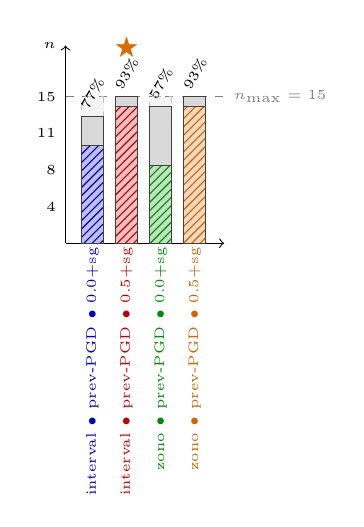
\begin{tikzpicture}[scale=0.62, every node/.style={font=\tiny}]
  \draw[->] (0,0) -- (3.25,0);
  \draw[->] (0,0) -- (0,4.05) node[left]{$n$};
  \draw[dashed, gray] (0,3.00) -- (3.25,3.00) node[right]{$n_{\max}=15$};
  \node[left, font=\tiny] at (0,0.75) {4};
  \node[left, font=\tiny] at (0,1.50) {8};
  \node[left, font=\tiny] at (0,2.25) {11};
  \node[left, font=\tiny] at (0,3.00) {15};
  \fill[gray!8] (0.33,0) rectangle (0.78,3.000);
  \draw[gray!50, line width=0.2pt, dashed] (0.33,0) rectangle (0.78,3.000);
  \fill[gray!30] (0.33,0) rectangle (0.78,2.600);
  \draw[gray!50!black, line width=0.2pt] (0.33,0) rectangle (0.78,2.600);
  \fill[white] (0.33,0.000) rectangle (0.78,2.000);
  \fill[blue!75!black, opacity=0.25] (0.33,0.000) rectangle (0.78,2.000);
  \fill[pattern=north east lines, pattern color=blue!75!black] (0.33,0.000) rectangle (0.78,2.000);
  \draw[gray!50!black, line width=0.2pt] (0.33,0.000) rectangle (0.78,2.000);
  \node[anchor=south west, rotate=60, font=\tiny, inner sep=1pt] at (0.50,2.620) {77\%};
  \node[anchor=east, rotate=90, font=\tiny, text=blue!75!black, inner sep=1pt] at (0.55,-0.02) {interval $\bullet$ prev-PGD $\bullet$ 0.0+sg};
  \fill[gray!8] (1.02,0) rectangle (1.48,3.000);
  \draw[gray!50, line width=0.2pt, dashed] (1.02,0) rectangle (1.48,3.000);
  \fill[gray!30] (1.02,0) rectangle (1.48,3.000);
  \draw[gray!50!black, line width=0.2pt] (1.02,0) rectangle (1.48,3.000);
  \fill[white] (1.02,0.000) rectangle (1.48,2.800);
  \fill[red!75!black, opacity=0.25] (1.02,0.000) rectangle (1.48,2.800);
  \fill[pattern=north east lines, pattern color=red!75!black] (1.02,0.000) rectangle (1.48,2.800);
  \draw[gray!50!black, line width=0.2pt] (1.02,0.000) rectangle (1.48,2.800);
  \node[anchor=south west, rotate=60, font=\tiny, inner sep=1pt] at (1.20,3.020) {93\%};
  \node[anchor=east, rotate=90, font=\tiny, text=red!75!black, inner sep=1pt] at (1.25,-0.02) {interval $\bullet$ prev-PGD $\bullet$ 0.5+sg};
  \fill[gray!8] (1.72,0) rectangle (2.17,3.000);
  \draw[gray!50, line width=0.2pt, dashed] (1.72,0) rectangle (2.17,3.000);
  \fill[gray!30] (1.72,0) rectangle (2.17,2.800);
  \draw[gray!50!black, line width=0.2pt] (1.72,0) rectangle (2.17,2.800);
  \fill[white] (1.72,0.000) rectangle (2.17,1.600);
  \fill[green!55!black, opacity=0.25] (1.72,0.000) rectangle (2.17,1.600);
  \fill[pattern=north east lines, pattern color=green!55!black] (1.72,0.000) rectangle (2.17,1.600);
  \draw[gray!50!black, line width=0.2pt] (1.72,0.000) rectangle (2.17,1.600);
  \node[anchor=south west, rotate=60, font=\tiny, inner sep=1pt] at (1.90,2.820) {57\%};
  \node[anchor=east, rotate=90, font=\tiny, text=green!55!black, inner sep=1pt] at (1.95,-0.02) {zono $\bullet$ prev-PGD $\bullet$ 0.0+sg};
  \fill[gray!8] (2.42,0) rectangle (2.87,3.000);
  \draw[gray!50, line width=0.2pt, dashed] (2.42,0) rectangle (2.87,3.000);
  \fill[gray!30] (2.42,0) rectangle (2.87,3.000);
  \draw[gray!50!black, line width=0.2pt] (2.42,0) rectangle (2.87,3.000);
  \fill[white] (2.42,0.000) rectangle (2.87,2.800);
  \fill[orange!80!black, opacity=0.25] (2.42,0.000) rectangle (2.87,2.800);
  \fill[pattern=north east lines, pattern color=orange!80!black] (2.42,0.000) rectangle (2.87,2.800);
  \draw[gray!50!black, line width=0.2pt] (2.42,0.000) rectangle (2.87,2.800);
  \node[anchor=south west, rotate=60, font=\tiny, inner sep=1pt] at (2.60,3.020) {93\%};
  \node[anchor=east, rotate=90, font=\tiny, text=orange!80!black, inner sep=1pt] at (2.65,-0.02) {zono $\bullet$ prev-PGD $\bullet$ 0.5+sg};
  \node[font=\small, text=orange!85!black] at (1.25,4.00) {$\bigstar$};
\end{tikzpicture}
\end{center}
\end{minipage}


\clearpage
\subsection*{Architecture \textbf{3x50} --- $\overline{\text{sp}}$ paired with win-rate}
\label{tab:perthist_3x50}
This page shows 4 paired rows, one per \textbf{perturbation type} measured on \textbf{3x50}. Each row repeats the same $\langle\text{arch}, \text{pert}\rangle$ slice twice: the \emph{left} chart is the mean-speedup view (section intro above); the \emph{right} chart is the win-rate view (same intro, different bar definition). Combo columns occupy the same x position in both charts of a row, so a column can be scanned down the page to follow one combo across perturbation types in both metrics.
\par\medskip\noindent
\begin{minipage}[t]{0.48\linewidth}
\begin{center}
\scriptsize
\colorbox{yellow!40}{\textbf{sp}}\;\textbf{3x50} \textbar{} pert \textbf{patch} (p\_sizes merged: \texttt{1,14,14,3}) \textbar{} 4 combos, total $n=72$ cells.\\[0.4ex]
\textbf{Ranking (best $\to$ worst):}\ \textcolor{orange!85!black}{$\bigstar$}\textcolor{blue!75!black}{\rule{0.55em}{0.55em}}\,1.09\,(1/1) ~ \textcolor{green!55!black}{\rule{0.55em}{0.55em}}\,1.04\,(1/1) ~ \textcolor{red!75!black}{\rule{0.55em}{0.55em}}\,1.04\,(1/1) ~ \textcolor{orange!80!black}{\rule{0.55em}{0.55em}}\,1.04\,(1/1)\\[0.4ex]
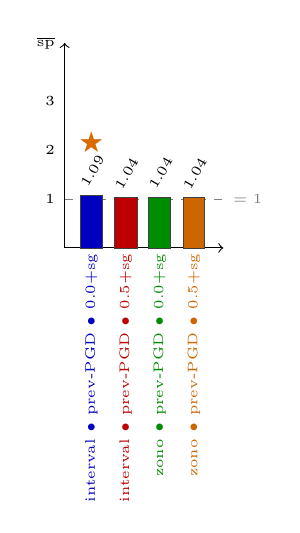
\begin{tikzpicture}[scale=0.62, every node/.style={font=\tiny}]
  \draw[->] (0,0) -- (3.25,0);
  \draw[->] (0,0) -- (0,4.20) node[left]{$\overline{\text{sp}}$};
  \draw[dashed, gray] (0,1) -- (3.25,1) node[right]{$=1$};
  \node[left, font=\tiny] at (0,1) {1};
  \node[left, font=\tiny] at (0,2) {2};
  \node[left, font=\tiny] at (0,3) {3};
  \fill[blue!75!black] (0.33,0) rectangle (0.78,1.085);
  \draw[gray!50!black, line width=0.2pt] (0.33,0) rectangle (0.78,1.085);
  \node[anchor=south west, rotate=60, font=\tiny, inner sep=1pt] at (0.50,1.135) {1.09};
  \node[anchor=east, rotate=90, font=\tiny, text=blue!75!black, inner sep=1pt] at (0.55,-0.05) {interval $\bullet$ prev-PGD $\bullet$ 0.0+sg};
  \fill[red!75!black] (1.02,0) rectangle (1.48,1.040);
  \draw[gray!50!black, line width=0.2pt] (1.02,0) rectangle (1.48,1.040);
  \node[anchor=south west, rotate=60, font=\tiny, inner sep=1pt] at (1.20,1.090) {1.04};
  \node[anchor=east, rotate=90, font=\tiny, text=red!75!black, inner sep=1pt] at (1.25,-0.05) {interval $\bullet$ prev-PGD $\bullet$ 0.5+sg};
  \fill[green!55!black] (1.72,0) rectangle (2.17,1.044);
  \draw[gray!50!black, line width=0.2pt] (1.72,0) rectangle (2.17,1.044);
  \node[anchor=south west, rotate=60, font=\tiny, inner sep=1pt] at (1.90,1.094) {1.04};
  \node[anchor=east, rotate=90, font=\tiny, text=green!55!black, inner sep=1pt] at (1.95,-0.05) {zono $\bullet$ prev-PGD $\bullet$ 0.0+sg};
  \fill[orange!80!black] (2.42,0) rectangle (2.87,1.039);
  \draw[gray!50!black, line width=0.2pt] (2.42,0) rectangle (2.87,1.039);
  \node[anchor=south west, rotate=60, font=\tiny, inner sep=1pt] at (2.60,1.089) {1.04};
  \node[anchor=east, rotate=90, font=\tiny, text=orange!80!black, inner sep=1pt] at (2.65,-0.05) {zono $\bullet$ prev-PGD $\bullet$ 0.5+sg};
  \node[font=\small, text=orange!85!black] at (0.55,2.14) {$\bigstar$};
\end{tikzpicture}
\end{center}
\end{minipage}
\hfill
\begin{minipage}[t]{0.48\linewidth}
\begin{center}
\scriptsize
\colorbox{cyan!30}{\textbf{win}}\;\textbf{3x50} \textbar{} pert \textbf{patch} (p\_sizes merged: \texttt{1,14,14,3}) \textbar{} 4 combos, total $n=72$ cells, $n_{\max}=18$.\\[0.4ex]
\textbf{Ranking (best $\to$ worst):}\ \textcolor{orange!85!black}{$\bigstar$}\textcolor{blue!75!black}{\rule{0.55em}{0.55em}}\,100\%\,(1f+17t/18) ~ \textcolor{red!75!black}{\rule{0.55em}{0.55em}}\,94\%\,(1f+16t/18) ~ \textcolor{green!55!black}{\rule{0.55em}{0.55em}}\,89\%\,(1f+15t/18) ~ \textcolor{orange!80!black}{\rule{0.55em}{0.55em}}\,89\%\,(1f+15t/18)\\[0.4ex]
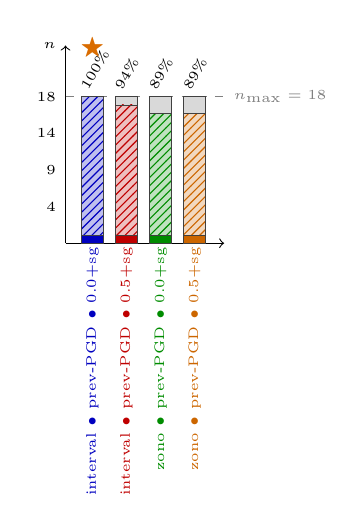
\begin{tikzpicture}[scale=0.62, every node/.style={font=\tiny}]
  \draw[->] (0,0) -- (3.25,0);
  \draw[->] (0,0) -- (0,4.05) node[left]{$n$};
  \draw[dashed, gray] (0,3.00) -- (3.25,3.00) node[right]{$n_{\max}=18$};
  \node[left, font=\tiny] at (0,0.75) {4};
  \node[left, font=\tiny] at (0,1.50) {9};
  \node[left, font=\tiny] at (0,2.25) {14};
  \node[left, font=\tiny] at (0,3.00) {18};
  \fill[gray!8] (0.33,0) rectangle (0.78,3.000);
  \draw[gray!50, line width=0.2pt, dashed] (0.33,0) rectangle (0.78,3.000);
  \fill[gray!30] (0.33,0) rectangle (0.78,3.000);
  \draw[gray!50!black, line width=0.2pt] (0.33,0) rectangle (0.78,3.000);
  \fill[blue!75!black] (0.33,0) rectangle (0.78,0.167);
  \draw[gray!50!black, line width=0.2pt] (0.33,0) rectangle (0.78,0.167);
  \fill[white] (0.33,0.167) rectangle (0.78,3.000);
  \fill[blue!75!black, opacity=0.25] (0.33,0.167) rectangle (0.78,3.000);
  \fill[pattern=north east lines, pattern color=blue!75!black] (0.33,0.167) rectangle (0.78,3.000);
  \draw[gray!50!black, line width=0.2pt] (0.33,0.167) rectangle (0.78,3.000);
  \node[anchor=south west, rotate=60, font=\tiny, inner sep=1pt] at (0.50,3.020) {100\%};
  \node[anchor=east, rotate=90, font=\tiny, text=blue!75!black, inner sep=1pt] at (0.55,-0.02) {interval $\bullet$ prev-PGD $\bullet$ 0.0+sg};
  \fill[gray!8] (1.02,0) rectangle (1.48,3.000);
  \draw[gray!50, line width=0.2pt, dashed] (1.02,0) rectangle (1.48,3.000);
  \fill[gray!30] (1.02,0) rectangle (1.48,3.000);
  \draw[gray!50!black, line width=0.2pt] (1.02,0) rectangle (1.48,3.000);
  \fill[red!75!black] (1.02,0) rectangle (1.48,0.167);
  \draw[gray!50!black, line width=0.2pt] (1.02,0) rectangle (1.48,0.167);
  \fill[white] (1.02,0.167) rectangle (1.48,2.833);
  \fill[red!75!black, opacity=0.25] (1.02,0.167) rectangle (1.48,2.833);
  \fill[pattern=north east lines, pattern color=red!75!black] (1.02,0.167) rectangle (1.48,2.833);
  \draw[gray!50!black, line width=0.2pt] (1.02,0.167) rectangle (1.48,2.833);
  \node[anchor=south west, rotate=60, font=\tiny, inner sep=1pt] at (1.20,3.020) {94\%};
  \node[anchor=east, rotate=90, font=\tiny, text=red!75!black, inner sep=1pt] at (1.25,-0.02) {interval $\bullet$ prev-PGD $\bullet$ 0.5+sg};
  \fill[gray!8] (1.72,0) rectangle (2.17,3.000);
  \draw[gray!50, line width=0.2pt, dashed] (1.72,0) rectangle (2.17,3.000);
  \fill[gray!30] (1.72,0) rectangle (2.17,3.000);
  \draw[gray!50!black, line width=0.2pt] (1.72,0) rectangle (2.17,3.000);
  \fill[green!55!black] (1.72,0) rectangle (2.17,0.167);
  \draw[gray!50!black, line width=0.2pt] (1.72,0) rectangle (2.17,0.167);
  \fill[white] (1.72,0.167) rectangle (2.17,2.667);
  \fill[green!55!black, opacity=0.25] (1.72,0.167) rectangle (2.17,2.667);
  \fill[pattern=north east lines, pattern color=green!55!black] (1.72,0.167) rectangle (2.17,2.667);
  \draw[gray!50!black, line width=0.2pt] (1.72,0.167) rectangle (2.17,2.667);
  \node[anchor=south west, rotate=60, font=\tiny, inner sep=1pt] at (1.90,3.020) {89\%};
  \node[anchor=east, rotate=90, font=\tiny, text=green!55!black, inner sep=1pt] at (1.95,-0.02) {zono $\bullet$ prev-PGD $\bullet$ 0.0+sg};
  \fill[gray!8] (2.42,0) rectangle (2.87,3.000);
  \draw[gray!50, line width=0.2pt, dashed] (2.42,0) rectangle (2.87,3.000);
  \fill[gray!30] (2.42,0) rectangle (2.87,3.000);
  \draw[gray!50!black, line width=0.2pt] (2.42,0) rectangle (2.87,3.000);
  \fill[orange!80!black] (2.42,0) rectangle (2.87,0.167);
  \draw[gray!50!black, line width=0.2pt] (2.42,0) rectangle (2.87,0.167);
  \fill[white] (2.42,0.167) rectangle (2.87,2.667);
  \fill[orange!80!black, opacity=0.25] (2.42,0.167) rectangle (2.87,2.667);
  \fill[pattern=north east lines, pattern color=orange!80!black] (2.42,0.167) rectangle (2.87,2.667);
  \draw[gray!50!black, line width=0.2pt] (2.42,0.167) rectangle (2.87,2.667);
  \node[anchor=south west, rotate=60, font=\tiny, inner sep=1pt] at (2.60,3.020) {89\%};
  \node[anchor=east, rotate=90, font=\tiny, text=orange!80!black, inner sep=1pt] at (2.65,-0.02) {zono $\bullet$ prev-PGD $\bullet$ 0.5+sg};
  \node[font=\small, text=orange!85!black] at (0.55,4.00) {$\bigstar$};
\end{tikzpicture}
\end{center}
\end{minipage}

\par\medskip\noindent
\begin{minipage}[t]{0.48\linewidth}
\begin{center}
\scriptsize
\colorbox{yellow!40}{\textbf{sp}}\;\textbf{3x50} \textbar{} pert \textbf{occ} (p\_sizes merged: \texttt{3,3,5}, \texttt{5,5,5}) \textbar{} 4 combos, total $n=142$ cells.\\[0.4ex]
\textbf{Ranking (best $\to$ worst):}\ \textcolor{orange!85!black}{$\bigstar$}\textcolor{green!55!black}{\rule{0.55em}{0.55em}}\,1.00\,(1/2) ~ \textcolor{blue!75!black}{\rule{0.55em}{0.55em}}\,1.00\,(1/2) ~ \textcolor{orange!80!black}{\rule{0.55em}{0.55em}}\,1.00\,(2/2) ~ \textcolor{red!75!black}{\rule{0.55em}{0.55em}}\,1.00\,(2/2)\\[0.4ex]
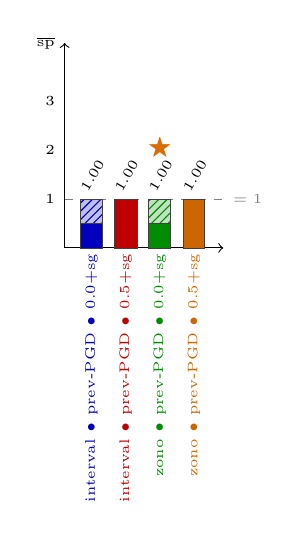
\begin{tikzpicture}[scale=0.62, every node/.style={font=\tiny}]
  \draw[->] (0,0) -- (3.25,0);
  \draw[->] (0,0) -- (0,4.20) node[left]{$\overline{\text{sp}}$};
  \draw[dashed, gray] (0,1) -- (3.25,1) node[right]{$=1$};
  \node[left, font=\tiny] at (0,1) {1};
  \node[left, font=\tiny] at (0,2) {2};
  \node[left, font=\tiny] at (0,3) {3};
  \fill[blue!75!black] (0.33,0) rectangle (0.78,0.500);
  \draw[gray!50!black, line width=0.2pt] (0.33,0) rectangle (0.78,0.500);
  \fill[blue!75!black, opacity=0.25] (0.33,0.500) rectangle (0.78,1.000);
  \fill[pattern=north east lines, pattern color=blue!75!black] (0.33,0.500) rectangle (0.78,1.000);
  \draw[gray!50!black, line width=0.2pt] (0.33,0.500) rectangle (0.78,1.000);
  \node[anchor=south west, rotate=60, font=\tiny, inner sep=1pt] at (0.50,1.050) {1.00};
  \node[anchor=east, rotate=90, font=\tiny, text=blue!75!black, inner sep=1pt] at (0.55,-0.05) {interval $\bullet$ prev-PGD $\bullet$ 0.0+sg};
  \fill[red!75!black] (1.02,0) rectangle (1.48,0.999);
  \draw[gray!50!black, line width=0.2pt] (1.02,0) rectangle (1.48,0.999);
  \node[anchor=south west, rotate=60, font=\tiny, inner sep=1pt] at (1.20,1.049) {1.00};
  \node[anchor=east, rotate=90, font=\tiny, text=red!75!black, inner sep=1pt] at (1.25,-0.05) {interval $\bullet$ prev-PGD $\bullet$ 0.5+sg};
  \fill[green!55!black] (1.72,0) rectangle (2.17,0.500);
  \draw[gray!50!black, line width=0.2pt] (1.72,0) rectangle (2.17,0.500);
  \fill[green!55!black, opacity=0.25] (1.72,0.500) rectangle (2.17,1.000);
  \fill[pattern=north east lines, pattern color=green!55!black] (1.72,0.500) rectangle (2.17,1.000);
  \draw[gray!50!black, line width=0.2pt] (1.72,0.500) rectangle (2.17,1.000);
  \node[anchor=south west, rotate=60, font=\tiny, inner sep=1pt] at (1.90,1.050) {1.00};
  \node[anchor=east, rotate=90, font=\tiny, text=green!55!black, inner sep=1pt] at (1.95,-0.05) {zono $\bullet$ prev-PGD $\bullet$ 0.0+sg};
  \fill[orange!80!black] (2.42,0) rectangle (2.87,0.999);
  \draw[gray!50!black, line width=0.2pt] (2.42,0) rectangle (2.87,0.999);
  \node[anchor=south west, rotate=60, font=\tiny, inner sep=1pt] at (2.60,1.049) {1.00};
  \node[anchor=east, rotate=90, font=\tiny, text=orange!80!black, inner sep=1pt] at (2.65,-0.05) {zono $\bullet$ prev-PGD $\bullet$ 0.5+sg};
  \node[font=\small, text=orange!85!black] at (1.95,2.05) {$\bigstar$};
\end{tikzpicture}
\end{center}
\end{minipage}
\hfill
\begin{minipage}[t]{0.48\linewidth}
\begin{center}
\scriptsize
\colorbox{cyan!30}{\textbf{win}}\;\textbf{3x50} \textbar{} pert \textbf{occ} (p\_sizes merged: \texttt{3,3,5}, \texttt{5,5,5}) \textbar{} 4 combos, total $n=142$ cells, $n_{\max}=36$.\\[0.4ex]
\textbf{Ranking (best $\to$ worst):}\ \textcolor{orange!85!black}{$\bigstar$}\textcolor{orange!80!black}{\rule{0.55em}{0.55em}}\,100\%\,(0f+36t/36) ~ \textcolor{red!75!black}{\rule{0.55em}{0.55em}}\,97\%\,(0f+35t/36) ~ \textcolor{blue!75!black}{\rule{0.55em}{0.55em}}\,66\%\,(0f+23t/35) ~ \textcolor{green!55!black}{\rule{0.55em}{0.55em}}\,57\%\,(0f+20t/35)\\[0.4ex]
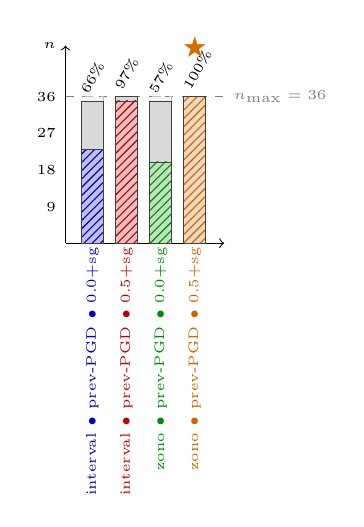
\begin{tikzpicture}[scale=0.62, every node/.style={font=\tiny}]
  \draw[->] (0,0) -- (3.25,0);
  \draw[->] (0,0) -- (0,4.05) node[left]{$n$};
  \draw[dashed, gray] (0,3.00) -- (3.25,3.00) node[right]{$n_{\max}=36$};
  \node[left, font=\tiny] at (0,0.75) {9};
  \node[left, font=\tiny] at (0,1.50) {18};
  \node[left, font=\tiny] at (0,2.25) {27};
  \node[left, font=\tiny] at (0,3.00) {36};
  \fill[gray!8] (0.33,0) rectangle (0.78,3.000);
  \draw[gray!50, line width=0.2pt, dashed] (0.33,0) rectangle (0.78,3.000);
  \fill[gray!30] (0.33,0) rectangle (0.78,2.917);
  \draw[gray!50!black, line width=0.2pt] (0.33,0) rectangle (0.78,2.917);
  \fill[white] (0.33,0.000) rectangle (0.78,1.917);
  \fill[blue!75!black, opacity=0.25] (0.33,0.000) rectangle (0.78,1.917);
  \fill[pattern=north east lines, pattern color=blue!75!black] (0.33,0.000) rectangle (0.78,1.917);
  \draw[gray!50!black, line width=0.2pt] (0.33,0.000) rectangle (0.78,1.917);
  \node[anchor=south west, rotate=60, font=\tiny, inner sep=1pt] at (0.50,2.937) {66\%};
  \node[anchor=east, rotate=90, font=\tiny, text=blue!75!black, inner sep=1pt] at (0.55,-0.02) {interval $\bullet$ prev-PGD $\bullet$ 0.0+sg};
  \fill[gray!8] (1.02,0) rectangle (1.48,3.000);
  \draw[gray!50, line width=0.2pt, dashed] (1.02,0) rectangle (1.48,3.000);
  \fill[gray!30] (1.02,0) rectangle (1.48,3.000);
  \draw[gray!50!black, line width=0.2pt] (1.02,0) rectangle (1.48,3.000);
  \fill[white] (1.02,0.000) rectangle (1.48,2.917);
  \fill[red!75!black, opacity=0.25] (1.02,0.000) rectangle (1.48,2.917);
  \fill[pattern=north east lines, pattern color=red!75!black] (1.02,0.000) rectangle (1.48,2.917);
  \draw[gray!50!black, line width=0.2pt] (1.02,0.000) rectangle (1.48,2.917);
  \node[anchor=south west, rotate=60, font=\tiny, inner sep=1pt] at (1.20,3.020) {97\%};
  \node[anchor=east, rotate=90, font=\tiny, text=red!75!black, inner sep=1pt] at (1.25,-0.02) {interval $\bullet$ prev-PGD $\bullet$ 0.5+sg};
  \fill[gray!8] (1.72,0) rectangle (2.17,3.000);
  \draw[gray!50, line width=0.2pt, dashed] (1.72,0) rectangle (2.17,3.000);
  \fill[gray!30] (1.72,0) rectangle (2.17,2.917);
  \draw[gray!50!black, line width=0.2pt] (1.72,0) rectangle (2.17,2.917);
  \fill[white] (1.72,0.000) rectangle (2.17,1.667);
  \fill[green!55!black, opacity=0.25] (1.72,0.000) rectangle (2.17,1.667);
  \fill[pattern=north east lines, pattern color=green!55!black] (1.72,0.000) rectangle (2.17,1.667);
  \draw[gray!50!black, line width=0.2pt] (1.72,0.000) rectangle (2.17,1.667);
  \node[anchor=south west, rotate=60, font=\tiny, inner sep=1pt] at (1.90,2.937) {57\%};
  \node[anchor=east, rotate=90, font=\tiny, text=green!55!black, inner sep=1pt] at (1.95,-0.02) {zono $\bullet$ prev-PGD $\bullet$ 0.0+sg};
  \fill[gray!8] (2.42,0) rectangle (2.87,3.000);
  \draw[gray!50, line width=0.2pt, dashed] (2.42,0) rectangle (2.87,3.000);
  \fill[gray!30] (2.42,0) rectangle (2.87,3.000);
  \draw[gray!50!black, line width=0.2pt] (2.42,0) rectangle (2.87,3.000);
  \fill[white] (2.42,0.000) rectangle (2.87,3.000);
  \fill[orange!80!black, opacity=0.25] (2.42,0.000) rectangle (2.87,3.000);
  \fill[pattern=north east lines, pattern color=orange!80!black] (2.42,0.000) rectangle (2.87,3.000);
  \draw[gray!50!black, line width=0.2pt] (2.42,0.000) rectangle (2.87,3.000);
  \node[anchor=south west, rotate=60, font=\tiny, inner sep=1pt] at (2.60,3.020) {100\%};
  \node[anchor=east, rotate=90, font=\tiny, text=orange!80!black, inner sep=1pt] at (2.65,-0.02) {zono $\bullet$ prev-PGD $\bullet$ 0.5+sg};
  \node[font=\small, text=orange!85!black] at (2.65,4.00) {$\bigstar$};
\end{tikzpicture}
\end{center}
\end{minipage}

\par\medskip\noindent
\begin{minipage}[t]{0.48\linewidth}
\begin{center}
\scriptsize
\colorbox{yellow!40}{\textbf{sp}}\;\textbf{3x50} \textbar{} pert \textbf{translation} (p\_sizes merged: \texttt{1,1}, \texttt{3,1}, \texttt{3,3}) \textbar{} 4 combos, total $n=216$ cells.\\[0.4ex]
\textbf{Ranking (best $\to$ worst):}\ \textcolor{orange!85!black}{$\bigstar$}\textcolor{red!75!black}{\rule{0.55em}{0.55em}}\,1.69\,(3/3) ~ \textcolor{orange!80!black}{\rule{0.55em}{0.55em}}\,1.69\,(3/3) ~ \textcolor{blue!75!black}{\rule{0.55em}{0.55em}}\,1.61\,(3/3) ~ \textcolor{green!55!black}{\rule{0.55em}{0.55em}}\,1.52\,(3/3)\\[0.4ex]
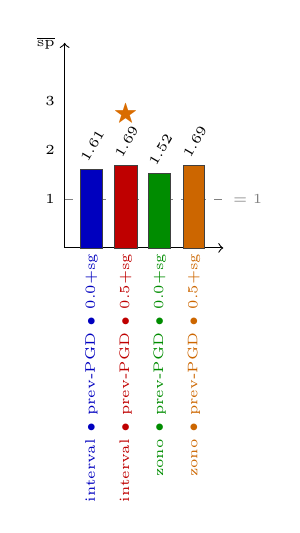
\begin{tikzpicture}[scale=0.62, every node/.style={font=\tiny}]
  \draw[->] (0,0) -- (3.25,0);
  \draw[->] (0,0) -- (0,4.20) node[left]{$\overline{\text{sp}}$};
  \draw[dashed, gray] (0,1) -- (3.25,1) node[right]{$=1$};
  \node[left, font=\tiny] at (0,1) {1};
  \node[left, font=\tiny] at (0,2) {2};
  \node[left, font=\tiny] at (0,3) {3};
  \fill[blue!75!black] (0.33,0) rectangle (0.78,1.614);
  \draw[gray!50!black, line width=0.2pt] (0.33,0) rectangle (0.78,1.614);
  \node[anchor=south west, rotate=60, font=\tiny, inner sep=1pt] at (0.50,1.664) {1.61};
  \node[anchor=east, rotate=90, font=\tiny, text=blue!75!black, inner sep=1pt] at (0.55,-0.05) {interval $\bullet$ prev-PGD $\bullet$ 0.0+sg};
  \fill[red!75!black] (1.02,0) rectangle (1.48,1.693);
  \draw[gray!50!black, line width=0.2pt] (1.02,0) rectangle (1.48,1.693);
  \node[anchor=south west, rotate=60, font=\tiny, inner sep=1pt] at (1.20,1.743) {1.69};
  \node[anchor=east, rotate=90, font=\tiny, text=red!75!black, inner sep=1pt] at (1.25,-0.05) {interval $\bullet$ prev-PGD $\bullet$ 0.5+sg};
  \fill[green!55!black] (1.72,0) rectangle (2.17,1.522);
  \draw[gray!50!black, line width=0.2pt] (1.72,0) rectangle (2.17,1.522);
  \node[anchor=south west, rotate=60, font=\tiny, inner sep=1pt] at (1.90,1.572) {1.52};
  \node[anchor=east, rotate=90, font=\tiny, text=green!55!black, inner sep=1pt] at (1.95,-0.05) {zono $\bullet$ prev-PGD $\bullet$ 0.0+sg};
  \fill[orange!80!black] (2.42,0) rectangle (2.87,1.693);
  \draw[gray!50!black, line width=0.2pt] (2.42,0) rectangle (2.87,1.693);
  \node[anchor=south west, rotate=60, font=\tiny, inner sep=1pt] at (2.60,1.743) {1.69};
  \node[anchor=east, rotate=90, font=\tiny, text=orange!80!black, inner sep=1pt] at (2.65,-0.05) {zono $\bullet$ prev-PGD $\bullet$ 0.5+sg};
  \node[font=\small, text=orange!85!black] at (1.25,2.74) {$\bigstar$};
\end{tikzpicture}
\end{center}
\end{minipage}
\hfill
\begin{minipage}[t]{0.48\linewidth}
\begin{center}
\scriptsize
\colorbox{cyan!30}{\textbf{win}}\;\textbf{3x50} \textbar{} pert \textbf{translation} (p\_sizes merged: \texttt{1,1}, \texttt{3,1}, \texttt{3,3}) \textbar{} 4 combos, total $n=216$ cells, $n_{\max}=54$.\\[0.4ex]
\textbf{Ranking (best $\to$ worst):}\ \textcolor{orange!85!black}{$\bigstar$}\textcolor{orange!80!black}{\rule{0.55em}{0.55em}}\,96\%\,(37f+15t/54) ~ \textcolor{green!55!black}{\rule{0.55em}{0.55em}}\,91\%\,(33f+16t/54) ~ \textcolor{red!75!black}{\rule{0.55em}{0.55em}}\,89\%\,(33f+15t/54) ~ \textcolor{blue!75!black}{\rule{0.55em}{0.55em}}\,87\%\,(32f+15t/54)\\[0.4ex]
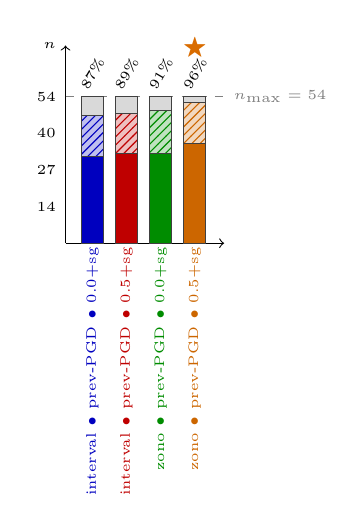
\begin{tikzpicture}[scale=0.62, every node/.style={font=\tiny}]
  \draw[->] (0,0) -- (3.25,0);
  \draw[->] (0,0) -- (0,4.05) node[left]{$n$};
  \draw[dashed, gray] (0,3.00) -- (3.25,3.00) node[right]{$n_{\max}=54$};
  \node[left, font=\tiny] at (0,0.75) {14};
  \node[left, font=\tiny] at (0,1.50) {27};
  \node[left, font=\tiny] at (0,2.25) {40};
  \node[left, font=\tiny] at (0,3.00) {54};
  \fill[gray!8] (0.33,0) rectangle (0.78,3.000);
  \draw[gray!50, line width=0.2pt, dashed] (0.33,0) rectangle (0.78,3.000);
  \fill[gray!30] (0.33,0) rectangle (0.78,3.000);
  \draw[gray!50!black, line width=0.2pt] (0.33,0) rectangle (0.78,3.000);
  \fill[blue!75!black] (0.33,0) rectangle (0.78,1.778);
  \draw[gray!50!black, line width=0.2pt] (0.33,0) rectangle (0.78,1.778);
  \fill[white] (0.33,1.778) rectangle (0.78,2.611);
  \fill[blue!75!black, opacity=0.25] (0.33,1.778) rectangle (0.78,2.611);
  \fill[pattern=north east lines, pattern color=blue!75!black] (0.33,1.778) rectangle (0.78,2.611);
  \draw[gray!50!black, line width=0.2pt] (0.33,1.778) rectangle (0.78,2.611);
  \node[anchor=south west, rotate=60, font=\tiny, inner sep=1pt] at (0.50,3.020) {87\%};
  \node[anchor=east, rotate=90, font=\tiny, text=blue!75!black, inner sep=1pt] at (0.55,-0.02) {interval $\bullet$ prev-PGD $\bullet$ 0.0+sg};
  \fill[gray!8] (1.02,0) rectangle (1.48,3.000);
  \draw[gray!50, line width=0.2pt, dashed] (1.02,0) rectangle (1.48,3.000);
  \fill[gray!30] (1.02,0) rectangle (1.48,3.000);
  \draw[gray!50!black, line width=0.2pt] (1.02,0) rectangle (1.48,3.000);
  \fill[red!75!black] (1.02,0) rectangle (1.48,1.833);
  \draw[gray!50!black, line width=0.2pt] (1.02,0) rectangle (1.48,1.833);
  \fill[white] (1.02,1.833) rectangle (1.48,2.667);
  \fill[red!75!black, opacity=0.25] (1.02,1.833) rectangle (1.48,2.667);
  \fill[pattern=north east lines, pattern color=red!75!black] (1.02,1.833) rectangle (1.48,2.667);
  \draw[gray!50!black, line width=0.2pt] (1.02,1.833) rectangle (1.48,2.667);
  \node[anchor=south west, rotate=60, font=\tiny, inner sep=1pt] at (1.20,3.020) {89\%};
  \node[anchor=east, rotate=90, font=\tiny, text=red!75!black, inner sep=1pt] at (1.25,-0.02) {interval $\bullet$ prev-PGD $\bullet$ 0.5+sg};
  \fill[gray!8] (1.72,0) rectangle (2.17,3.000);
  \draw[gray!50, line width=0.2pt, dashed] (1.72,0) rectangle (2.17,3.000);
  \fill[gray!30] (1.72,0) rectangle (2.17,3.000);
  \draw[gray!50!black, line width=0.2pt] (1.72,0) rectangle (2.17,3.000);
  \fill[green!55!black] (1.72,0) rectangle (2.17,1.833);
  \draw[gray!50!black, line width=0.2pt] (1.72,0) rectangle (2.17,1.833);
  \fill[white] (1.72,1.833) rectangle (2.17,2.722);
  \fill[green!55!black, opacity=0.25] (1.72,1.833) rectangle (2.17,2.722);
  \fill[pattern=north east lines, pattern color=green!55!black] (1.72,1.833) rectangle (2.17,2.722);
  \draw[gray!50!black, line width=0.2pt] (1.72,1.833) rectangle (2.17,2.722);
  \node[anchor=south west, rotate=60, font=\tiny, inner sep=1pt] at (1.90,3.020) {91\%};
  \node[anchor=east, rotate=90, font=\tiny, text=green!55!black, inner sep=1pt] at (1.95,-0.02) {zono $\bullet$ prev-PGD $\bullet$ 0.0+sg};
  \fill[gray!8] (2.42,0) rectangle (2.87,3.000);
  \draw[gray!50, line width=0.2pt, dashed] (2.42,0) rectangle (2.87,3.000);
  \fill[gray!30] (2.42,0) rectangle (2.87,3.000);
  \draw[gray!50!black, line width=0.2pt] (2.42,0) rectangle (2.87,3.000);
  \fill[orange!80!black] (2.42,0) rectangle (2.87,2.056);
  \draw[gray!50!black, line width=0.2pt] (2.42,0) rectangle (2.87,2.056);
  \fill[white] (2.42,2.056) rectangle (2.87,2.889);
  \fill[orange!80!black, opacity=0.25] (2.42,2.056) rectangle (2.87,2.889);
  \fill[pattern=north east lines, pattern color=orange!80!black] (2.42,2.056) rectangle (2.87,2.889);
  \draw[gray!50!black, line width=0.2pt] (2.42,2.056) rectangle (2.87,2.889);
  \node[anchor=south west, rotate=60, font=\tiny, inner sep=1pt] at (2.60,3.020) {96\%};
  \node[anchor=east, rotate=90, font=\tiny, text=orange!80!black, inner sep=1pt] at (2.65,-0.02) {zono $\bullet$ prev-PGD $\bullet$ 0.5+sg};
  \node[font=\small, text=orange!85!black] at (2.65,4.00) {$\bigstar$};
\end{tikzpicture}
\end{center}
\end{minipage}

\par\medskip\noindent
\begin{minipage}[t]{0.48\linewidth}
\begin{center}
\scriptsize
\colorbox{yellow!40}{\textbf{sp}}\;\textbf{3x50} \textbar{} pert \textbf{linf} (p\_sizes merged: \texttt{0.1}) \textbar{} 4 combos, total $n=70$ cells.\\[0.4ex]
\textbf{Ranking (best $\to$ worst):}\ \textcolor{orange!85!black}{$\bigstar$}\textcolor{orange!80!black}{\rule{0.55em}{0.55em}}\,1.00\,(1/1) ~ \textcolor{red!75!black}{\rule{0.55em}{0.55em}}\,1.00\,(1/1) ~ \textcolor{green!55!black}{\rule{0.55em}{0.55em}}\,1.00\,(1/1) ~ \textcolor{blue!75!black}{\rule{0.55em}{0.55em}}\,1.00\,(1/1)\\[0.4ex]
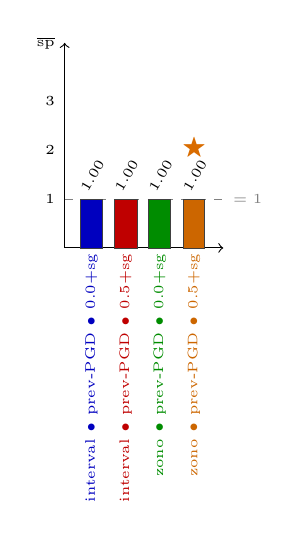
\begin{tikzpicture}[scale=0.62, every node/.style={font=\tiny}]
  \draw[->] (0,0) -- (3.25,0);
  \draw[->] (0,0) -- (0,4.20) node[left]{$\overline{\text{sp}}$};
  \draw[dashed, gray] (0,1) -- (3.25,1) node[right]{$=1$};
  \node[left, font=\tiny] at (0,1) {1};
  \node[left, font=\tiny] at (0,2) {2};
  \node[left, font=\tiny] at (0,3) {3};
  \fill[blue!75!black] (0.33,0) rectangle (0.78,0.999);
  \draw[gray!50!black, line width=0.2pt] (0.33,0) rectangle (0.78,0.999);
  \node[anchor=south west, rotate=60, font=\tiny, inner sep=1pt] at (0.50,1.049) {1.00};
  \node[anchor=east, rotate=90, font=\tiny, text=blue!75!black, inner sep=1pt] at (0.55,-0.05) {interval $\bullet$ prev-PGD $\bullet$ 0.0+sg};
  \fill[red!75!black] (1.02,0) rectangle (1.48,1.000);
  \draw[gray!50!black, line width=0.2pt] (1.02,0) rectangle (1.48,1.000);
  \node[anchor=south west, rotate=60, font=\tiny, inner sep=1pt] at (1.20,1.050) {1.00};
  \node[anchor=east, rotate=90, font=\tiny, text=red!75!black, inner sep=1pt] at (1.25,-0.05) {interval $\bullet$ prev-PGD $\bullet$ 0.5+sg};
  \fill[green!55!black] (1.72,0) rectangle (2.17,0.999);
  \draw[gray!50!black, line width=0.2pt] (1.72,0) rectangle (2.17,0.999);
  \node[anchor=south west, rotate=60, font=\tiny, inner sep=1pt] at (1.90,1.049) {1.00};
  \node[anchor=east, rotate=90, font=\tiny, text=green!55!black, inner sep=1pt] at (1.95,-0.05) {zono $\bullet$ prev-PGD $\bullet$ 0.0+sg};
  \fill[orange!80!black] (2.42,0) rectangle (2.87,1.000);
  \draw[gray!50!black, line width=0.2pt] (2.42,0) rectangle (2.87,1.000);
  \node[anchor=south west, rotate=60, font=\tiny, inner sep=1pt] at (2.60,1.050) {1.00};
  \node[anchor=east, rotate=90, font=\tiny, text=orange!80!black, inner sep=1pt] at (2.65,-0.05) {zono $\bullet$ prev-PGD $\bullet$ 0.5+sg};
  \node[font=\small, text=orange!85!black] at (2.65,2.05) {$\bigstar$};
\end{tikzpicture}
\end{center}
\end{minipage}
\hfill
\begin{minipage}[t]{0.48\linewidth}
\begin{center}
\scriptsize
\colorbox{cyan!30}{\textbf{win}}\;\textbf{3x50} \textbar{} pert \textbf{linf} (p\_sizes merged: \texttt{0.1}) \textbar{} 4 combos, total $n=70$ cells, $n_{\max}=18$.\\[0.4ex]
\textbf{Ranking (best $\to$ worst):}\ \textcolor{orange!85!black}{$\bigstar$}\textcolor{orange!80!black}{\rule{0.55em}{0.55em}}\,94\%\,(0f+17t/18) ~ \textcolor{red!75!black}{\rule{0.55em}{0.55em}}\,88\%\,(0f+15t/17) ~ \textcolor{blue!75!black}{\rule{0.55em}{0.55em}}\,78\%\,(0f+14t/18) ~ \textcolor{green!55!black}{\rule{0.55em}{0.55em}}\,76\%\,(0f+13t/17)\\[0.4ex]
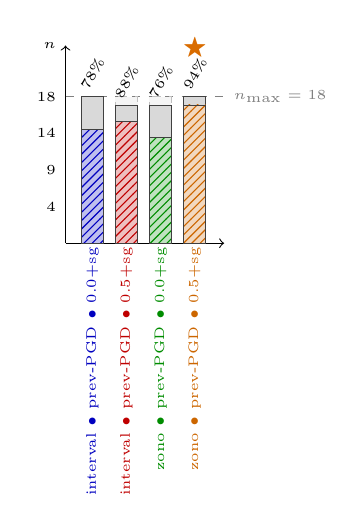
\begin{tikzpicture}[scale=0.62, every node/.style={font=\tiny}]
  \draw[->] (0,0) -- (3.25,0);
  \draw[->] (0,0) -- (0,4.05) node[left]{$n$};
  \draw[dashed, gray] (0,3.00) -- (3.25,3.00) node[right]{$n_{\max}=18$};
  \node[left, font=\tiny] at (0,0.75) {4};
  \node[left, font=\tiny] at (0,1.50) {9};
  \node[left, font=\tiny] at (0,2.25) {14};
  \node[left, font=\tiny] at (0,3.00) {18};
  \fill[gray!8] (0.33,0) rectangle (0.78,3.000);
  \draw[gray!50, line width=0.2pt, dashed] (0.33,0) rectangle (0.78,3.000);
  \fill[gray!30] (0.33,0) rectangle (0.78,3.000);
  \draw[gray!50!black, line width=0.2pt] (0.33,0) rectangle (0.78,3.000);
  \fill[white] (0.33,0.000) rectangle (0.78,2.333);
  \fill[blue!75!black, opacity=0.25] (0.33,0.000) rectangle (0.78,2.333);
  \fill[pattern=north east lines, pattern color=blue!75!black] (0.33,0.000) rectangle (0.78,2.333);
  \draw[gray!50!black, line width=0.2pt] (0.33,0.000) rectangle (0.78,2.333);
  \node[anchor=south west, rotate=60, font=\tiny, inner sep=1pt] at (0.50,3.020) {78\%};
  \node[anchor=east, rotate=90, font=\tiny, text=blue!75!black, inner sep=1pt] at (0.55,-0.02) {interval $\bullet$ prev-PGD $\bullet$ 0.0+sg};
  \fill[gray!8] (1.02,0) rectangle (1.48,3.000);
  \draw[gray!50, line width=0.2pt, dashed] (1.02,0) rectangle (1.48,3.000);
  \fill[gray!30] (1.02,0) rectangle (1.48,2.833);
  \draw[gray!50!black, line width=0.2pt] (1.02,0) rectangle (1.48,2.833);
  \fill[white] (1.02,0.000) rectangle (1.48,2.500);
  \fill[red!75!black, opacity=0.25] (1.02,0.000) rectangle (1.48,2.500);
  \fill[pattern=north east lines, pattern color=red!75!black] (1.02,0.000) rectangle (1.48,2.500);
  \draw[gray!50!black, line width=0.2pt] (1.02,0.000) rectangle (1.48,2.500);
  \node[anchor=south west, rotate=60, font=\tiny, inner sep=1pt] at (1.20,2.853) {88\%};
  \node[anchor=east, rotate=90, font=\tiny, text=red!75!black, inner sep=1pt] at (1.25,-0.02) {interval $\bullet$ prev-PGD $\bullet$ 0.5+sg};
  \fill[gray!8] (1.72,0) rectangle (2.17,3.000);
  \draw[gray!50, line width=0.2pt, dashed] (1.72,0) rectangle (2.17,3.000);
  \fill[gray!30] (1.72,0) rectangle (2.17,2.833);
  \draw[gray!50!black, line width=0.2pt] (1.72,0) rectangle (2.17,2.833);
  \fill[white] (1.72,0.000) rectangle (2.17,2.167);
  \fill[green!55!black, opacity=0.25] (1.72,0.000) rectangle (2.17,2.167);
  \fill[pattern=north east lines, pattern color=green!55!black] (1.72,0.000) rectangle (2.17,2.167);
  \draw[gray!50!black, line width=0.2pt] (1.72,0.000) rectangle (2.17,2.167);
  \node[anchor=south west, rotate=60, font=\tiny, inner sep=1pt] at (1.90,2.853) {76\%};
  \node[anchor=east, rotate=90, font=\tiny, text=green!55!black, inner sep=1pt] at (1.95,-0.02) {zono $\bullet$ prev-PGD $\bullet$ 0.0+sg};
  \fill[gray!8] (2.42,0) rectangle (2.87,3.000);
  \draw[gray!50, line width=0.2pt, dashed] (2.42,0) rectangle (2.87,3.000);
  \fill[gray!30] (2.42,0) rectangle (2.87,3.000);
  \draw[gray!50!black, line width=0.2pt] (2.42,0) rectangle (2.87,3.000);
  \fill[white] (2.42,0.000) rectangle (2.87,2.833);
  \fill[orange!80!black, opacity=0.25] (2.42,0.000) rectangle (2.87,2.833);
  \fill[pattern=north east lines, pattern color=orange!80!black] (2.42,0.000) rectangle (2.87,2.833);
  \draw[gray!50!black, line width=0.2pt] (2.42,0.000) rectangle (2.87,2.833);
  \node[anchor=south west, rotate=60, font=\tiny, inner sep=1pt] at (2.60,3.020) {94\%};
  \node[anchor=east, rotate=90, font=\tiny, text=orange!80!black, inner sep=1pt] at (2.65,-0.02) {zono $\bullet$ prev-PGD $\bullet$ 0.5+sg};
  \node[font=\small, text=orange!85!black] at (2.65,4.00) {$\bigstar$};
\end{tikzpicture}
\end{center}
\end{minipage}


\clearpage
\subsection*{Architecture \textbf{3x10} --- $\overline{\text{sp}}$ paired with win-rate}
\label{tab:perthist_3x10}
This page shows 4 paired rows, one per \textbf{perturbation type} measured on \textbf{3x10}. Each row repeats the same $\langle\text{arch}, \text{pert}\rangle$ slice twice: the \emph{left} chart is the mean-speedup view (section intro above); the \emph{right} chart is the win-rate view (same intro, different bar definition). Combo columns occupy the same x position in both charts of a row, so a column can be scanned down the page to follow one combo across perturbation types in both metrics.
\par\medskip\noindent
\begin{minipage}[t]{0.48\linewidth}
\begin{center}
\scriptsize
\colorbox{yellow!40}{\textbf{sp}}\;\textbf{3x10} \textbar{} pert \textbf{patch} (p\_sizes merged: \texttt{1,14,14,3}) \textbar{} 4 combos, total $n=108$ cells.\\[0.4ex]
\textbf{Ranking (best $\to$ worst):}\ \textcolor{orange!85!black}{$\bigstar$}\textcolor{blue!75!black}{\rule{0.55em}{0.55em}}\,1.18\,(1/1) ~ \textcolor{red!75!black}{\rule{0.55em}{0.55em}}\,1.17\,(1/1) ~ \textcolor{orange!80!black}{\rule{0.55em}{0.55em}}\,1.08\,(1/1) ~ \textcolor{green!55!black}{\rule{0.55em}{0.55em}}\,1.01\,(1/1)\\[0.4ex]
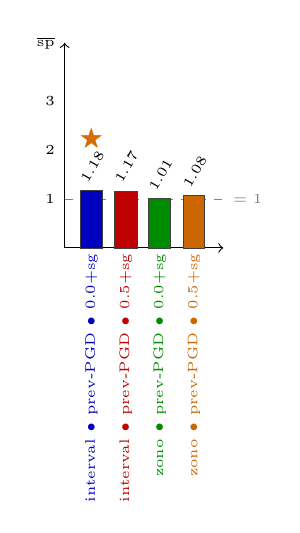
\begin{tikzpicture}[scale=0.62, every node/.style={font=\tiny}]
  \draw[->] (0,0) -- (3.25,0);
  \draw[->] (0,0) -- (0,4.20) node[left]{$\overline{\text{sp}}$};
  \draw[dashed, gray] (0,1) -- (3.25,1) node[right]{$=1$};
  \node[left, font=\tiny] at (0,1) {1};
  \node[left, font=\tiny] at (0,2) {2};
  \node[left, font=\tiny] at (0,3) {3};
  \fill[blue!75!black] (0.33,0) rectangle (0.78,1.183);
  \draw[gray!50!black, line width=0.2pt] (0.33,0) rectangle (0.78,1.183);
  \node[anchor=south west, rotate=60, font=\tiny, inner sep=1pt] at (0.50,1.233) {1.18};
  \node[anchor=east, rotate=90, font=\tiny, text=blue!75!black, inner sep=1pt] at (0.55,-0.05) {interval $\bullet$ prev-PGD $\bullet$ 0.0+sg};
  \fill[red!75!black] (1.02,0) rectangle (1.48,1.170);
  \draw[gray!50!black, line width=0.2pt] (1.02,0) rectangle (1.48,1.170);
  \node[anchor=south west, rotate=60, font=\tiny, inner sep=1pt] at (1.20,1.220) {1.17};
  \node[anchor=east, rotate=90, font=\tiny, text=red!75!black, inner sep=1pt] at (1.25,-0.05) {interval $\bullet$ prev-PGD $\bullet$ 0.5+sg};
  \fill[green!55!black] (1.72,0) rectangle (2.17,1.008);
  \draw[gray!50!black, line width=0.2pt] (1.72,0) rectangle (2.17,1.008);
  \node[anchor=south west, rotate=60, font=\tiny, inner sep=1pt] at (1.90,1.058) {1.01};
  \node[anchor=east, rotate=90, font=\tiny, text=green!55!black, inner sep=1pt] at (1.95,-0.05) {zono $\bullet$ prev-PGD $\bullet$ 0.0+sg};
  \fill[orange!80!black] (2.42,0) rectangle (2.87,1.078);
  \draw[gray!50!black, line width=0.2pt] (2.42,0) rectangle (2.87,1.078);
  \node[anchor=south west, rotate=60, font=\tiny, inner sep=1pt] at (2.60,1.128) {1.08};
  \node[anchor=east, rotate=90, font=\tiny, text=orange!80!black, inner sep=1pt] at (2.65,-0.05) {zono $\bullet$ prev-PGD $\bullet$ 0.5+sg};
  \node[font=\small, text=orange!85!black] at (0.55,2.23) {$\bigstar$};
\end{tikzpicture}
\end{center}
\end{minipage}
\hfill
\begin{minipage}[t]{0.48\linewidth}
\begin{center}
\scriptsize
\colorbox{cyan!30}{\textbf{win}}\;\textbf{3x10} \textbar{} pert \textbf{patch} (p\_sizes merged: \texttt{1,14,14,3}) \textbar{} 4 combos, total $n=108$ cells, $n_{\max}=27$.\\[0.4ex]
\textbf{Ranking (best $\to$ worst):}\ \textcolor{orange!85!black}{$\bigstar$}\textcolor{blue!75!black}{\rule{0.55em}{0.55em}}\,56\%\,(15f+0t/27) ~ \textcolor{red!75!black}{\rule{0.55em}{0.55em}}\,56\%\,(15f+0t/27) ~ \textcolor{orange!80!black}{\rule{0.55em}{0.55em}}\,52\%\,(14f+0t/27) ~ \textcolor{green!55!black}{\rule{0.55em}{0.55em}}\,44\%\,(12f+0t/27)\\[0.4ex]
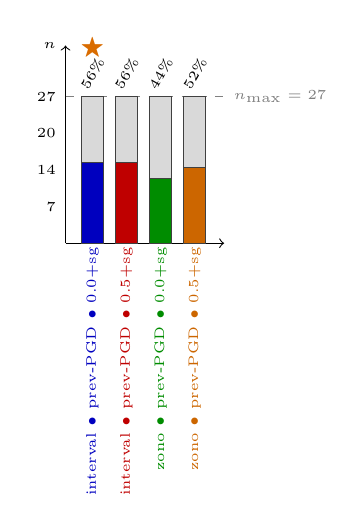
\begin{tikzpicture}[scale=0.62, every node/.style={font=\tiny}]
  \draw[->] (0,0) -- (3.25,0);
  \draw[->] (0,0) -- (0,4.05) node[left]{$n$};
  \draw[dashed, gray] (0,3.00) -- (3.25,3.00) node[right]{$n_{\max}=27$};
  \node[left, font=\tiny] at (0,0.75) {7};
  \node[left, font=\tiny] at (0,1.50) {14};
  \node[left, font=\tiny] at (0,2.25) {20};
  \node[left, font=\tiny] at (0,3.00) {27};
  \fill[gray!8] (0.33,0) rectangle (0.78,3.000);
  \draw[gray!50, line width=0.2pt, dashed] (0.33,0) rectangle (0.78,3.000);
  \fill[gray!30] (0.33,0) rectangle (0.78,3.000);
  \draw[gray!50!black, line width=0.2pt] (0.33,0) rectangle (0.78,3.000);
  \fill[blue!75!black] (0.33,0) rectangle (0.78,1.667);
  \draw[gray!50!black, line width=0.2pt] (0.33,0) rectangle (0.78,1.667);
  \node[anchor=south west, rotate=60, font=\tiny, inner sep=1pt] at (0.50,3.020) {56\%};
  \node[anchor=east, rotate=90, font=\tiny, text=blue!75!black, inner sep=1pt] at (0.55,-0.02) {interval $\bullet$ prev-PGD $\bullet$ 0.0+sg};
  \fill[gray!8] (1.02,0) rectangle (1.48,3.000);
  \draw[gray!50, line width=0.2pt, dashed] (1.02,0) rectangle (1.48,3.000);
  \fill[gray!30] (1.02,0) rectangle (1.48,3.000);
  \draw[gray!50!black, line width=0.2pt] (1.02,0) rectangle (1.48,3.000);
  \fill[red!75!black] (1.02,0) rectangle (1.48,1.667);
  \draw[gray!50!black, line width=0.2pt] (1.02,0) rectangle (1.48,1.667);
  \node[anchor=south west, rotate=60, font=\tiny, inner sep=1pt] at (1.20,3.020) {56\%};
  \node[anchor=east, rotate=90, font=\tiny, text=red!75!black, inner sep=1pt] at (1.25,-0.02) {interval $\bullet$ prev-PGD $\bullet$ 0.5+sg};
  \fill[gray!8] (1.72,0) rectangle (2.17,3.000);
  \draw[gray!50, line width=0.2pt, dashed] (1.72,0) rectangle (2.17,3.000);
  \fill[gray!30] (1.72,0) rectangle (2.17,3.000);
  \draw[gray!50!black, line width=0.2pt] (1.72,0) rectangle (2.17,3.000);
  \fill[green!55!black] (1.72,0) rectangle (2.17,1.333);
  \draw[gray!50!black, line width=0.2pt] (1.72,0) rectangle (2.17,1.333);
  \node[anchor=south west, rotate=60, font=\tiny, inner sep=1pt] at (1.90,3.020) {44\%};
  \node[anchor=east, rotate=90, font=\tiny, text=green!55!black, inner sep=1pt] at (1.95,-0.02) {zono $\bullet$ prev-PGD $\bullet$ 0.0+sg};
  \fill[gray!8] (2.42,0) rectangle (2.87,3.000);
  \draw[gray!50, line width=0.2pt, dashed] (2.42,0) rectangle (2.87,3.000);
  \fill[gray!30] (2.42,0) rectangle (2.87,3.000);
  \draw[gray!50!black, line width=0.2pt] (2.42,0) rectangle (2.87,3.000);
  \fill[orange!80!black] (2.42,0) rectangle (2.87,1.556);
  \draw[gray!50!black, line width=0.2pt] (2.42,0) rectangle (2.87,1.556);
  \node[anchor=south west, rotate=60, font=\tiny, inner sep=1pt] at (2.60,3.020) {52\%};
  \node[anchor=east, rotate=90, font=\tiny, text=orange!80!black, inner sep=1pt] at (2.65,-0.02) {zono $\bullet$ prev-PGD $\bullet$ 0.5+sg};
  \node[font=\small, text=orange!85!black] at (0.55,4.00) {$\bigstar$};
\end{tikzpicture}
\end{center}
\end{minipage}

\par\medskip\noindent
\begin{minipage}[t]{0.48\linewidth}
\begin{center}
\scriptsize
\colorbox{yellow!40}{\textbf{sp}}\;\textbf{3x10} \textbar{} pert \textbf{occ} (p\_sizes merged: \texttt{3,3,5}, \texttt{5,5,5}) \textbar{} 4 combos, total $n=180$ cells.\\[0.4ex]
\textbf{Ranking (best $\to$ worst):}\ \textcolor{orange!85!black}{$\bigstar$}\textcolor{blue!75!black}{\rule{0.55em}{0.55em}}\,1.21\,(2/2) ~ \textcolor{orange!80!black}{\rule{0.55em}{0.55em}}\,1.20\,(2/2) ~ \textcolor{red!75!black}{\rule{0.55em}{0.55em}}\,1.16\,(2/2) ~ \textcolor{green!55!black}{\rule{0.55em}{0.55em}}\,1.11\,(2/2)\\[0.4ex]
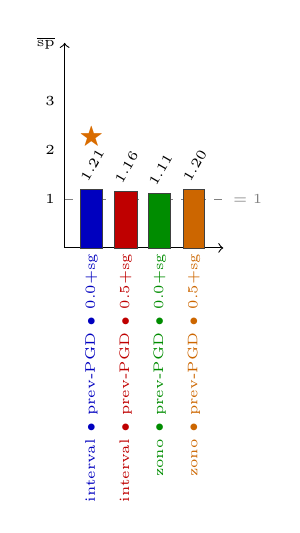
\begin{tikzpicture}[scale=0.62, every node/.style={font=\tiny}]
  \draw[->] (0,0) -- (3.25,0);
  \draw[->] (0,0) -- (0,4.20) node[left]{$\overline{\text{sp}}$};
  \draw[dashed, gray] (0,1) -- (3.25,1) node[right]{$=1$};
  \node[left, font=\tiny] at (0,1) {1};
  \node[left, font=\tiny] at (0,2) {2};
  \node[left, font=\tiny] at (0,3) {3};
  \fill[blue!75!black] (0.33,0) rectangle (0.78,1.205);
  \draw[gray!50!black, line width=0.2pt] (0.33,0) rectangle (0.78,1.205);
  \node[anchor=south west, rotate=60, font=\tiny, inner sep=1pt] at (0.50,1.255) {1.21};
  \node[anchor=east, rotate=90, font=\tiny, text=blue!75!black, inner sep=1pt] at (0.55,-0.05) {interval $\bullet$ prev-PGD $\bullet$ 0.0+sg};
  \fill[red!75!black] (1.02,0) rectangle (1.48,1.164);
  \draw[gray!50!black, line width=0.2pt] (1.02,0) rectangle (1.48,1.164);
  \node[anchor=south west, rotate=60, font=\tiny, inner sep=1pt] at (1.20,1.214) {1.16};
  \node[anchor=east, rotate=90, font=\tiny, text=red!75!black, inner sep=1pt] at (1.25,-0.05) {interval $\bullet$ prev-PGD $\bullet$ 0.5+sg};
  \fill[green!55!black] (1.72,0) rectangle (2.17,1.111);
  \draw[gray!50!black, line width=0.2pt] (1.72,0) rectangle (2.17,1.111);
  \node[anchor=south west, rotate=60, font=\tiny, inner sep=1pt] at (1.90,1.161) {1.11};
  \node[anchor=east, rotate=90, font=\tiny, text=green!55!black, inner sep=1pt] at (1.95,-0.05) {zono $\bullet$ prev-PGD $\bullet$ 0.0+sg};
  \fill[orange!80!black] (2.42,0) rectangle (2.87,1.203);
  \draw[gray!50!black, line width=0.2pt] (2.42,0) rectangle (2.87,1.203);
  \node[anchor=south west, rotate=60, font=\tiny, inner sep=1pt] at (2.60,1.253) {1.20};
  \node[anchor=east, rotate=90, font=\tiny, text=orange!80!black, inner sep=1pt] at (2.65,-0.05) {zono $\bullet$ prev-PGD $\bullet$ 0.5+sg};
  \node[font=\small, text=orange!85!black] at (0.55,2.26) {$\bigstar$};
\end{tikzpicture}
\end{center}
\end{minipage}
\hfill
\begin{minipage}[t]{0.48\linewidth}
\begin{center}
\scriptsize
\colorbox{cyan!30}{\textbf{win}}\;\textbf{3x10} \textbar{} pert \textbf{occ} (p\_sizes merged: \texttt{3,3,5}, \texttt{5,5,5}) \textbar{} 4 combos, total $n=180$ cells, $n_{\max}=54$.\\[0.4ex]
\textbf{Ranking (best $\to$ worst):}\ \textcolor{orange!85!black}{$\bigstar$}\textcolor{orange!80!black}{\rule{0.55em}{0.55em}}\,70\%\,(38f+0t/54) ~ \textcolor{red!75!black}{\rule{0.55em}{0.55em}}\,69\%\,(25f+0t/36) ~ \textcolor{green!55!black}{\rule{0.55em}{0.55em}}\,67\%\,(36f+0t/54) ~ \textcolor{blue!75!black}{\rule{0.55em}{0.55em}}\,61\%\,(22f+0t/36)\\[0.4ex]
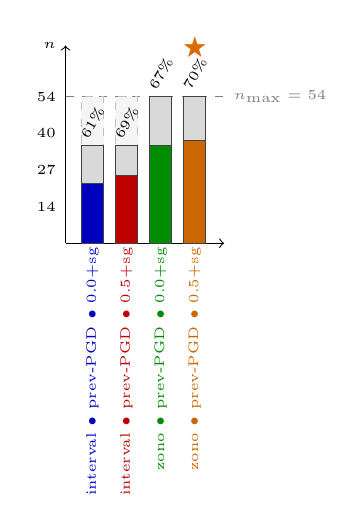
\begin{tikzpicture}[scale=0.62, every node/.style={font=\tiny}]
  \draw[->] (0,0) -- (3.25,0);
  \draw[->] (0,0) -- (0,4.05) node[left]{$n$};
  \draw[dashed, gray] (0,3.00) -- (3.25,3.00) node[right]{$n_{\max}=54$};
  \node[left, font=\tiny] at (0,0.75) {14};
  \node[left, font=\tiny] at (0,1.50) {27};
  \node[left, font=\tiny] at (0,2.25) {40};
  \node[left, font=\tiny] at (0,3.00) {54};
  \fill[gray!8] (0.33,0) rectangle (0.78,3.000);
  \draw[gray!50, line width=0.2pt, dashed] (0.33,0) rectangle (0.78,3.000);
  \fill[gray!30] (0.33,0) rectangle (0.78,2.000);
  \draw[gray!50!black, line width=0.2pt] (0.33,0) rectangle (0.78,2.000);
  \fill[blue!75!black] (0.33,0) rectangle (0.78,1.222);
  \draw[gray!50!black, line width=0.2pt] (0.33,0) rectangle (0.78,1.222);
  \node[anchor=south west, rotate=60, font=\tiny, inner sep=1pt] at (0.50,2.020) {61\%};
  \node[anchor=east, rotate=90, font=\tiny, text=blue!75!black, inner sep=1pt] at (0.55,-0.02) {interval $\bullet$ prev-PGD $\bullet$ 0.0+sg};
  \fill[gray!8] (1.02,0) rectangle (1.48,3.000);
  \draw[gray!50, line width=0.2pt, dashed] (1.02,0) rectangle (1.48,3.000);
  \fill[gray!30] (1.02,0) rectangle (1.48,2.000);
  \draw[gray!50!black, line width=0.2pt] (1.02,0) rectangle (1.48,2.000);
  \fill[red!75!black] (1.02,0) rectangle (1.48,1.389);
  \draw[gray!50!black, line width=0.2pt] (1.02,0) rectangle (1.48,1.389);
  \node[anchor=south west, rotate=60, font=\tiny, inner sep=1pt] at (1.20,2.020) {69\%};
  \node[anchor=east, rotate=90, font=\tiny, text=red!75!black, inner sep=1pt] at (1.25,-0.02) {interval $\bullet$ prev-PGD $\bullet$ 0.5+sg};
  \fill[gray!8] (1.72,0) rectangle (2.17,3.000);
  \draw[gray!50, line width=0.2pt, dashed] (1.72,0) rectangle (2.17,3.000);
  \fill[gray!30] (1.72,0) rectangle (2.17,3.000);
  \draw[gray!50!black, line width=0.2pt] (1.72,0) rectangle (2.17,3.000);
  \fill[green!55!black] (1.72,0) rectangle (2.17,2.000);
  \draw[gray!50!black, line width=0.2pt] (1.72,0) rectangle (2.17,2.000);
  \node[anchor=south west, rotate=60, font=\tiny, inner sep=1pt] at (1.90,3.020) {67\%};
  \node[anchor=east, rotate=90, font=\tiny, text=green!55!black, inner sep=1pt] at (1.95,-0.02) {zono $\bullet$ prev-PGD $\bullet$ 0.0+sg};
  \fill[gray!8] (2.42,0) rectangle (2.87,3.000);
  \draw[gray!50, line width=0.2pt, dashed] (2.42,0) rectangle (2.87,3.000);
  \fill[gray!30] (2.42,0) rectangle (2.87,3.000);
  \draw[gray!50!black, line width=0.2pt] (2.42,0) rectangle (2.87,3.000);
  \fill[orange!80!black] (2.42,0) rectangle (2.87,2.111);
  \draw[gray!50!black, line width=0.2pt] (2.42,0) rectangle (2.87,2.111);
  \node[anchor=south west, rotate=60, font=\tiny, inner sep=1pt] at (2.60,3.020) {70\%};
  \node[anchor=east, rotate=90, font=\tiny, text=orange!80!black, inner sep=1pt] at (2.65,-0.02) {zono $\bullet$ prev-PGD $\bullet$ 0.5+sg};
  \node[font=\small, text=orange!85!black] at (2.65,4.00) {$\bigstar$};
\end{tikzpicture}
\end{center}
\end{minipage}

\par\medskip\noindent
\begin{minipage}[t]{0.48\linewidth}
\begin{center}
\scriptsize
\colorbox{yellow!40}{\textbf{sp}}\;\textbf{3x10} \textbar{} pert \textbf{translation} (p\_sizes merged: \texttt{1,1}, \texttt{3,1}, \texttt{3,3}) \textbar{} 4 combos, total $n=291$ cells.\\[0.4ex]
\textbf{Ranking (best $\to$ worst):}\ \textcolor{orange!85!black}{$\bigstar$}\textcolor{red!75!black}{\rule{0.55em}{0.55em}}\,1.33\,(3/3) ~ \textcolor{green!55!black}{\rule{0.55em}{0.55em}}\,1.23\,(3/3) ~ \textcolor{blue!75!black}{\rule{0.55em}{0.55em}}\,1.22\,(3/3) ~ \textcolor{orange!80!black}{\rule{0.55em}{0.55em}}\,1.22\,(3/3)\\[0.4ex]
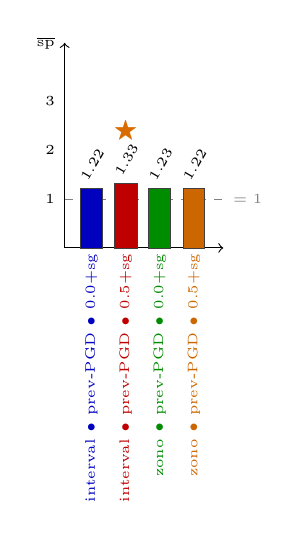
\begin{tikzpicture}[scale=0.62, every node/.style={font=\tiny}]
  \draw[->] (0,0) -- (3.25,0);
  \draw[->] (0,0) -- (0,4.20) node[left]{$\overline{\text{sp}}$};
  \draw[dashed, gray] (0,1) -- (3.25,1) node[right]{$=1$};
  \node[left, font=\tiny] at (0,1) {1};
  \node[left, font=\tiny] at (0,2) {2};
  \node[left, font=\tiny] at (0,3) {3};
  \fill[blue!75!black] (0.33,0) rectangle (0.78,1.223);
  \draw[gray!50!black, line width=0.2pt] (0.33,0) rectangle (0.78,1.223);
  \node[anchor=south west, rotate=60, font=\tiny, inner sep=1pt] at (0.50,1.273) {1.22};
  \node[anchor=east, rotate=90, font=\tiny, text=blue!75!black, inner sep=1pt] at (0.55,-0.05) {interval $\bullet$ prev-PGD $\bullet$ 0.0+sg};
  \fill[red!75!black] (1.02,0) rectangle (1.48,1.325);
  \draw[gray!50!black, line width=0.2pt] (1.02,0) rectangle (1.48,1.325);
  \node[anchor=south west, rotate=60, font=\tiny, inner sep=1pt] at (1.20,1.375) {1.33};
  \node[anchor=east, rotate=90, font=\tiny, text=red!75!black, inner sep=1pt] at (1.25,-0.05) {interval $\bullet$ prev-PGD $\bullet$ 0.5+sg};
  \fill[green!55!black] (1.72,0) rectangle (2.17,1.226);
  \draw[gray!50!black, line width=0.2pt] (1.72,0) rectangle (2.17,1.226);
  \node[anchor=south west, rotate=60, font=\tiny, inner sep=1pt] at (1.90,1.276) {1.23};
  \node[anchor=east, rotate=90, font=\tiny, text=green!55!black, inner sep=1pt] at (1.95,-0.05) {zono $\bullet$ prev-PGD $\bullet$ 0.0+sg};
  \fill[orange!80!black] (2.42,0) rectangle (2.87,1.221);
  \draw[gray!50!black, line width=0.2pt] (2.42,0) rectangle (2.87,1.221);
  \node[anchor=south west, rotate=60, font=\tiny, inner sep=1pt] at (2.60,1.271) {1.22};
  \node[anchor=east, rotate=90, font=\tiny, text=orange!80!black, inner sep=1pt] at (2.65,-0.05) {zono $\bullet$ prev-PGD $\bullet$ 0.5+sg};
  \node[font=\small, text=orange!85!black] at (1.25,2.38) {$\bigstar$};
\end{tikzpicture}
\end{center}
\end{minipage}
\hfill
\begin{minipage}[t]{0.48\linewidth}
\begin{center}
\scriptsize
\colorbox{cyan!30}{\textbf{win}}\;\textbf{3x10} \textbar{} pert \textbf{translation} (p\_sizes merged: \texttt{1,1}, \texttt{3,1}, \texttt{3,3}) \textbar{} 4 combos, total $n=291$ cells, $n_{\max}=81$.\\[0.4ex]
\textbf{Ranking (best $\to$ worst):}\ \textcolor{orange!85!black}{$\bigstar$}\textcolor{red!75!black}{\rule{0.55em}{0.55em}}\,79\%\,(48f+0t/61) ~ \textcolor{orange!80!black}{\rule{0.55em}{0.55em}}\,70\%\,(57f+0t/81) ~ \textcolor{green!55!black}{\rule{0.55em}{0.55em}}\,69\%\,(56f+0t/81) ~ \textcolor{blue!75!black}{\rule{0.55em}{0.55em}}\,66\%\,(45f+0t/68)\\[0.4ex]
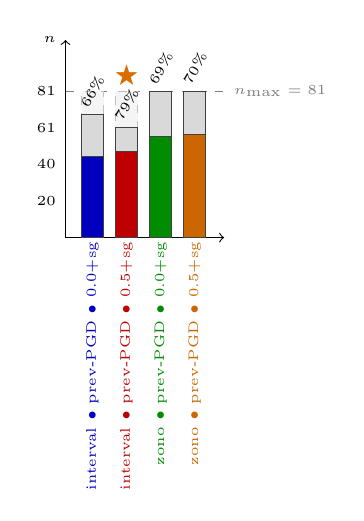
\begin{tikzpicture}[scale=0.62, every node/.style={font=\tiny}]
  \draw[->] (0,0) -- (3.25,0);
  \draw[->] (0,0) -- (0,4.05) node[left]{$n$};
  \draw[dashed, gray] (0,3.00) -- (3.25,3.00) node[right]{$n_{\max}=81$};
  \node[left, font=\tiny] at (0,0.75) {20};
  \node[left, font=\tiny] at (0,1.50) {40};
  \node[left, font=\tiny] at (0,2.25) {61};
  \node[left, font=\tiny] at (0,3.00) {81};
  \fill[gray!8] (0.33,0) rectangle (0.78,3.000);
  \draw[gray!50, line width=0.2pt, dashed] (0.33,0) rectangle (0.78,3.000);
  \fill[gray!30] (0.33,0) rectangle (0.78,2.519);
  \draw[gray!50!black, line width=0.2pt] (0.33,0) rectangle (0.78,2.519);
  \fill[blue!75!black] (0.33,0) rectangle (0.78,1.667);
  \draw[gray!50!black, line width=0.2pt] (0.33,0) rectangle (0.78,1.667);
  \node[anchor=south west, rotate=60, font=\tiny, inner sep=1pt] at (0.50,2.539) {66\%};
  \node[anchor=east, rotate=90, font=\tiny, text=blue!75!black, inner sep=1pt] at (0.55,-0.02) {interval $\bullet$ prev-PGD $\bullet$ 0.0+sg};
  \fill[gray!8] (1.02,0) rectangle (1.48,3.000);
  \draw[gray!50, line width=0.2pt, dashed] (1.02,0) rectangle (1.48,3.000);
  \fill[gray!30] (1.02,0) rectangle (1.48,2.259);
  \draw[gray!50!black, line width=0.2pt] (1.02,0) rectangle (1.48,2.259);
  \fill[red!75!black] (1.02,0) rectangle (1.48,1.778);
  \draw[gray!50!black, line width=0.2pt] (1.02,0) rectangle (1.48,1.778);
  \node[anchor=south west, rotate=60, font=\tiny, inner sep=1pt] at (1.20,2.279) {79\%};
  \node[anchor=east, rotate=90, font=\tiny, text=red!75!black, inner sep=1pt] at (1.25,-0.02) {interval $\bullet$ prev-PGD $\bullet$ 0.5+sg};
  \fill[gray!8] (1.72,0) rectangle (2.17,3.000);
  \draw[gray!50, line width=0.2pt, dashed] (1.72,0) rectangle (2.17,3.000);
  \fill[gray!30] (1.72,0) rectangle (2.17,3.000);
  \draw[gray!50!black, line width=0.2pt] (1.72,0) rectangle (2.17,3.000);
  \fill[green!55!black] (1.72,0) rectangle (2.17,2.074);
  \draw[gray!50!black, line width=0.2pt] (1.72,0) rectangle (2.17,2.074);
  \node[anchor=south west, rotate=60, font=\tiny, inner sep=1pt] at (1.90,3.020) {69\%};
  \node[anchor=east, rotate=90, font=\tiny, text=green!55!black, inner sep=1pt] at (1.95,-0.02) {zono $\bullet$ prev-PGD $\bullet$ 0.0+sg};
  \fill[gray!8] (2.42,0) rectangle (2.87,3.000);
  \draw[gray!50, line width=0.2pt, dashed] (2.42,0) rectangle (2.87,3.000);
  \fill[gray!30] (2.42,0) rectangle (2.87,3.000);
  \draw[gray!50!black, line width=0.2pt] (2.42,0) rectangle (2.87,3.000);
  \fill[orange!80!black] (2.42,0) rectangle (2.87,2.111);
  \draw[gray!50!black, line width=0.2pt] (2.42,0) rectangle (2.87,2.111);
  \node[anchor=south west, rotate=60, font=\tiny, inner sep=1pt] at (2.60,3.020) {70\%};
  \node[anchor=east, rotate=90, font=\tiny, text=orange!80!black, inner sep=1pt] at (2.65,-0.02) {zono $\bullet$ prev-PGD $\bullet$ 0.5+sg};
  \node[font=\small, text=orange!85!black] at (1.25,3.31) {$\bigstar$};
\end{tikzpicture}
\end{center}
\end{minipage}

\par\medskip\noindent
\begin{minipage}[t]{0.48\linewidth}
\begin{center}
\scriptsize
\colorbox{yellow!40}{\textbf{sp}}\;\textbf{3x10} \textbar{} pert \textbf{linf} (p\_sizes merged: \texttt{0.1}) \textbar{} 4 combos, total $n=90$ cells.\\[0.4ex]
\textbf{Ranking (best $\to$ worst):}\ \textcolor{orange!85!black}{$\bigstar$}\textcolor{blue!75!black}{\rule{0.55em}{0.55em}}\,1.16\,(1/1) ~ \textcolor{red!75!black}{\rule{0.55em}{0.55em}}\,1.14\,(1/1) ~ \textcolor{green!55!black}{\rule{0.55em}{0.55em}}\,1.07\,(1/1) ~ \textcolor{orange!80!black}{\rule{0.55em}{0.55em}}\,0.98\,(0/1)\\[0.4ex]
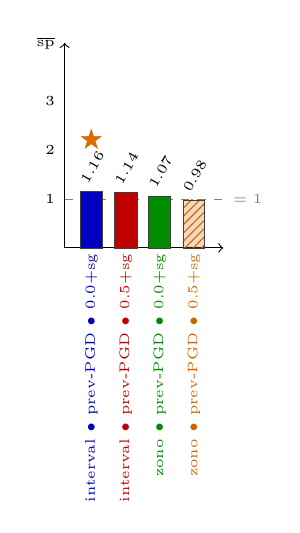
\begin{tikzpicture}[scale=0.62, every node/.style={font=\tiny}]
  \draw[->] (0,0) -- (3.25,0);
  \draw[->] (0,0) -- (0,4.20) node[left]{$\overline{\text{sp}}$};
  \draw[dashed, gray] (0,1) -- (3.25,1) node[right]{$=1$};
  \node[left, font=\tiny] at (0,1) {1};
  \node[left, font=\tiny] at (0,2) {2};
  \node[left, font=\tiny] at (0,3) {3};
  \fill[blue!75!black] (0.33,0) rectangle (0.78,1.164);
  \draw[gray!50!black, line width=0.2pt] (0.33,0) rectangle (0.78,1.164);
  \node[anchor=south west, rotate=60, font=\tiny, inner sep=1pt] at (0.50,1.214) {1.16};
  \node[anchor=east, rotate=90, font=\tiny, text=blue!75!black, inner sep=1pt] at (0.55,-0.05) {interval $\bullet$ prev-PGD $\bullet$ 0.0+sg};
  \fill[red!75!black] (1.02,0) rectangle (1.48,1.144);
  \draw[gray!50!black, line width=0.2pt] (1.02,0) rectangle (1.48,1.144);
  \node[anchor=south west, rotate=60, font=\tiny, inner sep=1pt] at (1.20,1.194) {1.14};
  \node[anchor=east, rotate=90, font=\tiny, text=red!75!black, inner sep=1pt] at (1.25,-0.05) {interval $\bullet$ prev-PGD $\bullet$ 0.5+sg};
  \fill[green!55!black] (1.72,0) rectangle (2.17,1.067);
  \draw[gray!50!black, line width=0.2pt] (1.72,0) rectangle (2.17,1.067);
  \node[anchor=south west, rotate=60, font=\tiny, inner sep=1pt] at (1.90,1.117) {1.07};
  \node[anchor=east, rotate=90, font=\tiny, text=green!55!black, inner sep=1pt] at (1.95,-0.05) {zono $\bullet$ prev-PGD $\bullet$ 0.0+sg};
  \fill[orange!80!black, opacity=0.25] (2.42,0.000) rectangle (2.87,0.983);
  \fill[pattern=north east lines, pattern color=orange!80!black] (2.42,0.000) rectangle (2.87,0.983);
  \draw[gray!50!black, line width=0.2pt] (2.42,0.000) rectangle (2.87,0.983);
  \node[anchor=south west, rotate=60, font=\tiny, inner sep=1pt] at (2.60,1.033) {0.98};
  \node[anchor=east, rotate=90, font=\tiny, text=orange!80!black, inner sep=1pt] at (2.65,-0.05) {zono $\bullet$ prev-PGD $\bullet$ 0.5+sg};
  \node[font=\small, text=orange!85!black] at (0.55,2.21) {$\bigstar$};
\end{tikzpicture}
\end{center}
\end{minipage}
\hfill
\begin{minipage}[t]{0.48\linewidth}
\begin{center}
\scriptsize
\colorbox{cyan!30}{\textbf{win}}\;\textbf{3x10} \textbar{} pert \textbf{linf} (p\_sizes merged: \texttt{0.1}) \textbar{} 4 combos, total $n=90$ cells, $n_{\max}=27$.\\[0.4ex]
\textbf{Ranking (best $\to$ worst):}\ \textcolor{orange!85!black}{$\bigstar$}\textcolor{blue!75!black}{\rule{0.55em}{0.55em}}\,61\%\,(11f+0t/18) ~ \textcolor{red!75!black}{\rule{0.55em}{0.55em}}\,61\%\,(11f+0t/18) ~ \textcolor{green!55!black}{\rule{0.55em}{0.55em}}\,56\%\,(15f+0t/27) ~ \textcolor{orange!80!black}{\rule{0.55em}{0.55em}}\,44\%\,(12f+0t/27)\\[0.4ex]
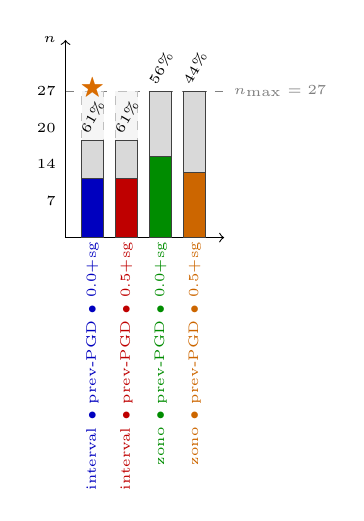
\begin{tikzpicture}[scale=0.62, every node/.style={font=\tiny}]
  \draw[->] (0,0) -- (3.25,0);
  \draw[->] (0,0) -- (0,4.05) node[left]{$n$};
  \draw[dashed, gray] (0,3.00) -- (3.25,3.00) node[right]{$n_{\max}=27$};
  \node[left, font=\tiny] at (0,0.75) {7};
  \node[left, font=\tiny] at (0,1.50) {14};
  \node[left, font=\tiny] at (0,2.25) {20};
  \node[left, font=\tiny] at (0,3.00) {27};
  \fill[gray!8] (0.33,0) rectangle (0.78,3.000);
  \draw[gray!50, line width=0.2pt, dashed] (0.33,0) rectangle (0.78,3.000);
  \fill[gray!30] (0.33,0) rectangle (0.78,2.000);
  \draw[gray!50!black, line width=0.2pt] (0.33,0) rectangle (0.78,2.000);
  \fill[blue!75!black] (0.33,0) rectangle (0.78,1.222);
  \draw[gray!50!black, line width=0.2pt] (0.33,0) rectangle (0.78,1.222);
  \node[anchor=south west, rotate=60, font=\tiny, inner sep=1pt] at (0.50,2.020) {61\%};
  \node[anchor=east, rotate=90, font=\tiny, text=blue!75!black, inner sep=1pt] at (0.55,-0.02) {interval $\bullet$ prev-PGD $\bullet$ 0.0+sg};
  \fill[gray!8] (1.02,0) rectangle (1.48,3.000);
  \draw[gray!50, line width=0.2pt, dashed] (1.02,0) rectangle (1.48,3.000);
  \fill[gray!30] (1.02,0) rectangle (1.48,2.000);
  \draw[gray!50!black, line width=0.2pt] (1.02,0) rectangle (1.48,2.000);
  \fill[red!75!black] (1.02,0) rectangle (1.48,1.222);
  \draw[gray!50!black, line width=0.2pt] (1.02,0) rectangle (1.48,1.222);
  \node[anchor=south west, rotate=60, font=\tiny, inner sep=1pt] at (1.20,2.020) {61\%};
  \node[anchor=east, rotate=90, font=\tiny, text=red!75!black, inner sep=1pt] at (1.25,-0.02) {interval $\bullet$ prev-PGD $\bullet$ 0.5+sg};
  \fill[gray!8] (1.72,0) rectangle (2.17,3.000);
  \draw[gray!50, line width=0.2pt, dashed] (1.72,0) rectangle (2.17,3.000);
  \fill[gray!30] (1.72,0) rectangle (2.17,3.000);
  \draw[gray!50!black, line width=0.2pt] (1.72,0) rectangle (2.17,3.000);
  \fill[green!55!black] (1.72,0) rectangle (2.17,1.667);
  \draw[gray!50!black, line width=0.2pt] (1.72,0) rectangle (2.17,1.667);
  \node[anchor=south west, rotate=60, font=\tiny, inner sep=1pt] at (1.90,3.020) {56\%};
  \node[anchor=east, rotate=90, font=\tiny, text=green!55!black, inner sep=1pt] at (1.95,-0.02) {zono $\bullet$ prev-PGD $\bullet$ 0.0+sg};
  \fill[gray!8] (2.42,0) rectangle (2.87,3.000);
  \draw[gray!50, line width=0.2pt, dashed] (2.42,0) rectangle (2.87,3.000);
  \fill[gray!30] (2.42,0) rectangle (2.87,3.000);
  \draw[gray!50!black, line width=0.2pt] (2.42,0) rectangle (2.87,3.000);
  \fill[orange!80!black] (2.42,0) rectangle (2.87,1.333);
  \draw[gray!50!black, line width=0.2pt] (2.42,0) rectangle (2.87,1.333);
  \node[anchor=south west, rotate=60, font=\tiny, inner sep=1pt] at (2.60,3.020) {44\%};
  \node[anchor=east, rotate=90, font=\tiny, text=orange!80!black, inner sep=1pt] at (2.65,-0.02) {zono $\bullet$ prev-PGD $\bullet$ 0.5+sg};
  \node[font=\small, text=orange!85!black] at (0.55,3.05) {$\bigstar$};
\end{tikzpicture}
\end{center}
\end{minipage}

\clearpage
\section*{Per-perturbation histograms across all architectures: $\overline{\text{sp}}$ paired with win-rate}
This section pools every $(c_\mathrm{src}, c_\mathrm{tgt}, \text{seed})$ cell across \emph{all} measured architectures, so each paired row reports a combo's behaviour on one perturbation type aggregated over every arch we ran. Bar definitions, the ★ best-combo marker, and the rules used to split each bar into solid + hatched segments are exactly the same as in the per-arch section above. Architecture is shown as \textbf{ALL} in each chart's caption.
\noindent\textbf{Note:} these histograms are restricted to the 4 combinations \texttt{zono:prev\_pgd:0.0+sg}, \texttt{zono:prev\_pgd:0.5+sg}, \texttt{interval:prev\_pgd:0.0+sg}, \texttt{interval:prev\_pgd:0.5+sg} (via \texttt{--combination\_table}).
\par\medskip\noindent
\begin{minipage}[t]{0.48\linewidth}
\begin{center}
\scriptsize
\colorbox{yellow!40}{\textbf{sp}}\;\textbf{ALL} \textbar{} pert \textbf{patch} (p\_sizes merged: \texttt{1,14,14,3}) \textbar{} 4 combos, total $n=270$ cells.\\[0.4ex]
\textbf{Ranking (best $\to$ worst):}\ \textcolor{orange!85!black}{$\bigstar$}\textcolor{orange!80!black}{\rule{0.55em}{0.55em}}\,1.46\,(1/1) ~ \textcolor{red!75!black}{\rule{0.55em}{0.55em}}\,1.34\,(1/1) ~ \textcolor{green!55!black}{\rule{0.55em}{0.55em}}\,1.26\,(1/1) ~ \textcolor{blue!75!black}{\rule{0.55em}{0.55em}}\,1.22\,(1/1)\\[0.4ex]
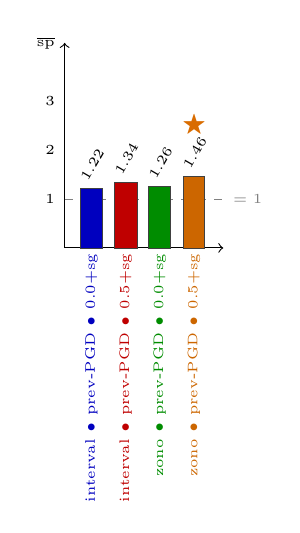
\begin{tikzpicture}[scale=0.62, every node/.style={font=\tiny}]
  \draw[->] (0,0) -- (3.25,0);
  \draw[->] (0,0) -- (0,4.20) node[left]{$\overline{\text{sp}}$};
  \draw[dashed, gray] (0,1) -- (3.25,1) node[right]{$=1$};
  \node[left, font=\tiny] at (0,1) {1};
  \node[left, font=\tiny] at (0,2) {2};
  \node[left, font=\tiny] at (0,3) {3};
  \fill[blue!75!black] (0.33,0) rectangle (0.78,1.220);
  \draw[gray!50!black, line width=0.2pt] (0.33,0) rectangle (0.78,1.220);
  \node[anchor=south west, rotate=60, font=\tiny, inner sep=1pt] at (0.50,1.270) {1.22};
  \node[anchor=east, rotate=90, font=\tiny, text=blue!75!black, inner sep=1pt] at (0.55,-0.05) {interval $\bullet$ prev-PGD $\bullet$ 0.0+sg};
  \fill[red!75!black] (1.02,0) rectangle (1.48,1.337);
  \draw[gray!50!black, line width=0.2pt] (1.02,0) rectangle (1.48,1.337);
  \node[anchor=south west, rotate=60, font=\tiny, inner sep=1pt] at (1.20,1.387) {1.34};
  \node[anchor=east, rotate=90, font=\tiny, text=red!75!black, inner sep=1pt] at (1.25,-0.05) {interval $\bullet$ prev-PGD $\bullet$ 0.5+sg};
  \fill[green!55!black] (1.72,0) rectangle (2.17,1.263);
  \draw[gray!50!black, line width=0.2pt] (1.72,0) rectangle (2.17,1.263);
  \node[anchor=south west, rotate=60, font=\tiny, inner sep=1pt] at (1.90,1.313) {1.26};
  \node[anchor=east, rotate=90, font=\tiny, text=green!55!black, inner sep=1pt] at (1.95,-0.05) {zono $\bullet$ prev-PGD $\bullet$ 0.0+sg};
  \fill[orange!80!black] (2.42,0) rectangle (2.87,1.464);
  \draw[gray!50!black, line width=0.2pt] (2.42,0) rectangle (2.87,1.464);
  \node[anchor=south west, rotate=60, font=\tiny, inner sep=1pt] at (2.60,1.514) {1.46};
  \node[anchor=east, rotate=90, font=\tiny, text=orange!80!black, inner sep=1pt] at (2.65,-0.05) {zono $\bullet$ prev-PGD $\bullet$ 0.5+sg};
  \node[font=\small, text=orange!85!black] at (2.65,2.51) {$\bigstar$};
\end{tikzpicture}
\end{center}
\end{minipage}
\hfill
\begin{minipage}[t]{0.48\linewidth}
\begin{center}
\scriptsize
\colorbox{cyan!30}{\textbf{win}}\;\textbf{ALL} \textbar{} pert \textbf{patch} (p\_sizes merged: \texttt{1,14,14,3}) \textbar{} 4 combos, total $n=270$ cells, $n_{\max}=72$.\\[0.4ex]
\textbf{Ranking (best $\to$ worst):}\ \textcolor{orange!85!black}{$\bigstar$}\textcolor{red!75!black}{\rule{0.55em}{0.55em}}\,76\%\,(32f+16t/63) ~ \textcolor{orange!80!black}{\rule{0.55em}{0.55em}}\,75\%\,(39f+15t/72) ~ \textcolor{blue!75!black}{\rule{0.55em}{0.55em}}\,73\%\,(29f+17t/63) ~ \textcolor{green!55!black}{\rule{0.55em}{0.55em}}\,64\%\,(31f+15t/72)\\[0.4ex]
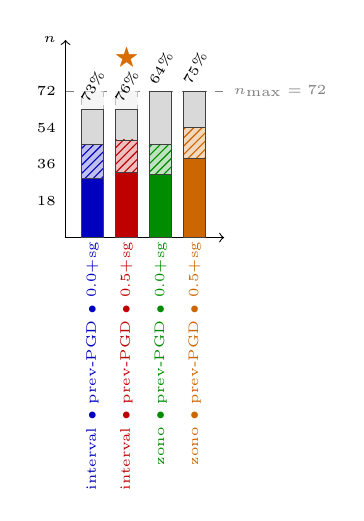
\begin{tikzpicture}[scale=0.62, every node/.style={font=\tiny}]
  \draw[->] (0,0) -- (3.25,0);
  \draw[->] (0,0) -- (0,4.05) node[left]{$n$};
  \draw[dashed, gray] (0,3.00) -- (3.25,3.00) node[right]{$n_{\max}=72$};
  \node[left, font=\tiny] at (0,0.75) {18};
  \node[left, font=\tiny] at (0,1.50) {36};
  \node[left, font=\tiny] at (0,2.25) {54};
  \node[left, font=\tiny] at (0,3.00) {72};
  \fill[gray!8] (0.33,0) rectangle (0.78,3.000);
  \draw[gray!50, line width=0.2pt, dashed] (0.33,0) rectangle (0.78,3.000);
  \fill[gray!30] (0.33,0) rectangle (0.78,2.625);
  \draw[gray!50!black, line width=0.2pt] (0.33,0) rectangle (0.78,2.625);
  \fill[blue!75!black] (0.33,0) rectangle (0.78,1.208);
  \draw[gray!50!black, line width=0.2pt] (0.33,0) rectangle (0.78,1.208);
  \fill[white] (0.33,1.208) rectangle (0.78,1.917);
  \fill[blue!75!black, opacity=0.25] (0.33,1.208) rectangle (0.78,1.917);
  \fill[pattern=north east lines, pattern color=blue!75!black] (0.33,1.208) rectangle (0.78,1.917);
  \draw[gray!50!black, line width=0.2pt] (0.33,1.208) rectangle (0.78,1.917);
  \node[anchor=south west, rotate=60, font=\tiny, inner sep=1pt] at (0.50,2.645) {73\%};
  \node[anchor=east, rotate=90, font=\tiny, text=blue!75!black, inner sep=1pt] at (0.55,-0.02) {interval $\bullet$ prev-PGD $\bullet$ 0.0+sg};
  \fill[gray!8] (1.02,0) rectangle (1.48,3.000);
  \draw[gray!50, line width=0.2pt, dashed] (1.02,0) rectangle (1.48,3.000);
  \fill[gray!30] (1.02,0) rectangle (1.48,2.625);
  \draw[gray!50!black, line width=0.2pt] (1.02,0) rectangle (1.48,2.625);
  \fill[red!75!black] (1.02,0) rectangle (1.48,1.333);
  \draw[gray!50!black, line width=0.2pt] (1.02,0) rectangle (1.48,1.333);
  \fill[white] (1.02,1.333) rectangle (1.48,2.000);
  \fill[red!75!black, opacity=0.25] (1.02,1.333) rectangle (1.48,2.000);
  \fill[pattern=north east lines, pattern color=red!75!black] (1.02,1.333) rectangle (1.48,2.000);
  \draw[gray!50!black, line width=0.2pt] (1.02,1.333) rectangle (1.48,2.000);
  \node[anchor=south west, rotate=60, font=\tiny, inner sep=1pt] at (1.20,2.645) {76\%};
  \node[anchor=east, rotate=90, font=\tiny, text=red!75!black, inner sep=1pt] at (1.25,-0.02) {interval $\bullet$ prev-PGD $\bullet$ 0.5+sg};
  \fill[gray!8] (1.72,0) rectangle (2.17,3.000);
  \draw[gray!50, line width=0.2pt, dashed] (1.72,0) rectangle (2.17,3.000);
  \fill[gray!30] (1.72,0) rectangle (2.17,3.000);
  \draw[gray!50!black, line width=0.2pt] (1.72,0) rectangle (2.17,3.000);
  \fill[green!55!black] (1.72,0) rectangle (2.17,1.292);
  \draw[gray!50!black, line width=0.2pt] (1.72,0) rectangle (2.17,1.292);
  \fill[white] (1.72,1.292) rectangle (2.17,1.917);
  \fill[green!55!black, opacity=0.25] (1.72,1.292) rectangle (2.17,1.917);
  \fill[pattern=north east lines, pattern color=green!55!black] (1.72,1.292) rectangle (2.17,1.917);
  \draw[gray!50!black, line width=0.2pt] (1.72,1.292) rectangle (2.17,1.917);
  \node[anchor=south west, rotate=60, font=\tiny, inner sep=1pt] at (1.90,3.020) {64\%};
  \node[anchor=east, rotate=90, font=\tiny, text=green!55!black, inner sep=1pt] at (1.95,-0.02) {zono $\bullet$ prev-PGD $\bullet$ 0.0+sg};
  \fill[gray!8] (2.42,0) rectangle (2.87,3.000);
  \draw[gray!50, line width=0.2pt, dashed] (2.42,0) rectangle (2.87,3.000);
  \fill[gray!30] (2.42,0) rectangle (2.87,3.000);
  \draw[gray!50!black, line width=0.2pt] (2.42,0) rectangle (2.87,3.000);
  \fill[orange!80!black] (2.42,0) rectangle (2.87,1.625);
  \draw[gray!50!black, line width=0.2pt] (2.42,0) rectangle (2.87,1.625);
  \fill[white] (2.42,1.625) rectangle (2.87,2.250);
  \fill[orange!80!black, opacity=0.25] (2.42,1.625) rectangle (2.87,2.250);
  \fill[pattern=north east lines, pattern color=orange!80!black] (2.42,1.625) rectangle (2.87,2.250);
  \draw[gray!50!black, line width=0.2pt] (2.42,1.625) rectangle (2.87,2.250);
  \node[anchor=south west, rotate=60, font=\tiny, inner sep=1pt] at (2.60,3.020) {75\%};
  \node[anchor=east, rotate=90, font=\tiny, text=orange!80!black, inner sep=1pt] at (2.65,-0.02) {zono $\bullet$ prev-PGD $\bullet$ 0.5+sg};
  \node[font=\small, text=orange!85!black] at (1.25,3.67) {$\bigstar$};
\end{tikzpicture}
\end{center}
\end{minipage}

\par\medskip\noindent
\begin{minipage}[t]{0.48\linewidth}
\begin{center}
\scriptsize
\colorbox{yellow!40}{\textbf{sp}}\;\textbf{ALL} \textbar{} pert \textbf{occ} (p\_sizes merged: \texttt{3,3,5}, \texttt{5,5,5}) \textbar{} 4 combos, total $n=475$ cells.\\[0.4ex]
\textbf{Ranking (best $\to$ worst):}\ \textcolor{orange!85!black}{$\bigstar$}\textcolor{blue!75!black}{\rule{0.55em}{0.55em}}\,1.42\,(2/2) ~ \textcolor{red!75!black}{\rule{0.55em}{0.55em}}\,1.40\,(2/2) ~ \textcolor{orange!80!black}{\rule{0.55em}{0.55em}}\,1.31\,(2/2) ~ \textcolor{green!55!black}{\rule{0.55em}{0.55em}}\,1.31\,(2/2)\\[0.4ex]
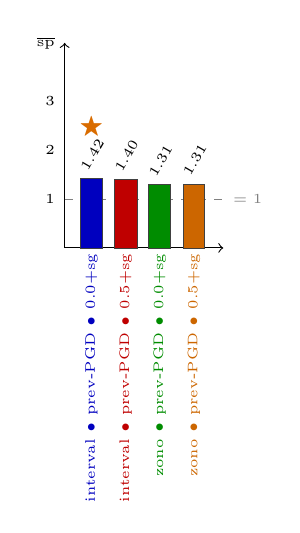
\begin{tikzpicture}[scale=0.62, every node/.style={font=\tiny}]
  \draw[->] (0,0) -- (3.25,0);
  \draw[->] (0,0) -- (0,4.20) node[left]{$\overline{\text{sp}}$};
  \draw[dashed, gray] (0,1) -- (3.25,1) node[right]{$=1$};
  \node[left, font=\tiny] at (0,1) {1};
  \node[left, font=\tiny] at (0,2) {2};
  \node[left, font=\tiny] at (0,3) {3};
  \fill[blue!75!black] (0.33,0) rectangle (0.78,1.423);
  \draw[gray!50!black, line width=0.2pt] (0.33,0) rectangle (0.78,1.423);
  \node[anchor=south west, rotate=60, font=\tiny, inner sep=1pt] at (0.50,1.473) {1.42};
  \node[anchor=east, rotate=90, font=\tiny, text=blue!75!black, inner sep=1pt] at (0.55,-0.05) {interval $\bullet$ prev-PGD $\bullet$ 0.0+sg};
  \fill[red!75!black] (1.02,0) rectangle (1.48,1.398);
  \draw[gray!50!black, line width=0.2pt] (1.02,0) rectangle (1.48,1.398);
  \node[anchor=south west, rotate=60, font=\tiny, inner sep=1pt] at (1.20,1.448) {1.40};
  \node[anchor=east, rotate=90, font=\tiny, text=red!75!black, inner sep=1pt] at (1.25,-0.05) {interval $\bullet$ prev-PGD $\bullet$ 0.5+sg};
  \fill[green!55!black] (1.72,0) rectangle (2.17,1.306);
  \draw[gray!50!black, line width=0.2pt] (1.72,0) rectangle (2.17,1.306);
  \node[anchor=south west, rotate=60, font=\tiny, inner sep=1pt] at (1.90,1.356) {1.31};
  \node[anchor=east, rotate=90, font=\tiny, text=green!55!black, inner sep=1pt] at (1.95,-0.05) {zono $\bullet$ prev-PGD $\bullet$ 0.0+sg};
  \fill[orange!80!black] (2.42,0) rectangle (2.87,1.312);
  \draw[gray!50!black, line width=0.2pt] (2.42,0) rectangle (2.87,1.312);
  \node[anchor=south west, rotate=60, font=\tiny, inner sep=1pt] at (2.60,1.362) {1.31};
  \node[anchor=east, rotate=90, font=\tiny, text=orange!80!black, inner sep=1pt] at (2.65,-0.05) {zono $\bullet$ prev-PGD $\bullet$ 0.5+sg};
  \node[font=\small, text=orange!85!black] at (0.55,2.47) {$\bigstar$};
\end{tikzpicture}
\end{center}
\end{minipage}
\hfill
\begin{minipage}[t]{0.48\linewidth}
\begin{center}
\scriptsize
\colorbox{cyan!30}{\textbf{win}}\;\textbf{ALL} \textbar{} pert \textbf{occ} (p\_sizes merged: \texttt{3,3,5}, \texttt{5,5,5}) \textbar{} 4 combos, total $n=475$ cells, $n_{\max}=134$.\\[0.4ex]
\textbf{Ranking (best $\to$ worst):}\ \textcolor{orange!85!black}{$\bigstar$}\textcolor{orange!80!black}{\rule{0.55em}{0.55em}}\,77\%\,(61f+36t/126) ~ \textcolor{red!75!black}{\rule{0.55em}{0.55em}}\,77\%\,(48f+35t/108) ~ \textcolor{green!55!black}{\rule{0.55em}{0.55em}}\,61\%\,(62f+20t/134) ~ \textcolor{blue!75!black}{\rule{0.55em}{0.55em}}\,61\%\,(42f+23t/107)\\[0.4ex]
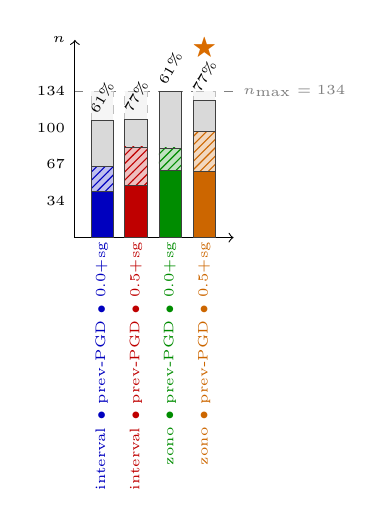
\begin{tikzpicture}[scale=0.62, every node/.style={font=\tiny}]
  \draw[->] (0,0) -- (3.25,0);
  \draw[->] (0,0) -- (0,4.05) node[left]{$n$};
  \draw[dashed, gray] (0,3.00) -- (3.25,3.00) node[right]{$n_{\max}=134$};
  \node[left, font=\tiny] at (0,0.75) {34};
  \node[left, font=\tiny] at (0,1.50) {67};
  \node[left, font=\tiny] at (0,2.25) {100};
  \node[left, font=\tiny] at (0,3.00) {134};
  \fill[gray!8] (0.33,0) rectangle (0.78,3.000);
  \draw[gray!50, line width=0.2pt, dashed] (0.33,0) rectangle (0.78,3.000);
  \fill[gray!30] (0.33,0) rectangle (0.78,2.396);
  \draw[gray!50!black, line width=0.2pt] (0.33,0) rectangle (0.78,2.396);
  \fill[blue!75!black] (0.33,0) rectangle (0.78,0.940);
  \draw[gray!50!black, line width=0.2pt] (0.33,0) rectangle (0.78,0.940);
  \fill[white] (0.33,0.940) rectangle (0.78,1.455);
  \fill[blue!75!black, opacity=0.25] (0.33,0.940) rectangle (0.78,1.455);
  \fill[pattern=north east lines, pattern color=blue!75!black] (0.33,0.940) rectangle (0.78,1.455);
  \draw[gray!50!black, line width=0.2pt] (0.33,0.940) rectangle (0.78,1.455);
  \node[anchor=south west, rotate=60, font=\tiny, inner sep=1pt] at (0.50,2.416) {61\%};
  \node[anchor=east, rotate=90, font=\tiny, text=blue!75!black, inner sep=1pt] at (0.55,-0.02) {interval $\bullet$ prev-PGD $\bullet$ 0.0+sg};
  \fill[gray!8] (1.02,0) rectangle (1.48,3.000);
  \draw[gray!50, line width=0.2pt, dashed] (1.02,0) rectangle (1.48,3.000);
  \fill[gray!30] (1.02,0) rectangle (1.48,2.418);
  \draw[gray!50!black, line width=0.2pt] (1.02,0) rectangle (1.48,2.418);
  \fill[red!75!black] (1.02,0) rectangle (1.48,1.075);
  \draw[gray!50!black, line width=0.2pt] (1.02,0) rectangle (1.48,1.075);
  \fill[white] (1.02,1.075) rectangle (1.48,1.858);
  \fill[red!75!black, opacity=0.25] (1.02,1.075) rectangle (1.48,1.858);
  \fill[pattern=north east lines, pattern color=red!75!black] (1.02,1.075) rectangle (1.48,1.858);
  \draw[gray!50!black, line width=0.2pt] (1.02,1.075) rectangle (1.48,1.858);
  \node[anchor=south west, rotate=60, font=\tiny, inner sep=1pt] at (1.20,2.438) {77\%};
  \node[anchor=east, rotate=90, font=\tiny, text=red!75!black, inner sep=1pt] at (1.25,-0.02) {interval $\bullet$ prev-PGD $\bullet$ 0.5+sg};
  \fill[gray!8] (1.72,0) rectangle (2.17,3.000);
  \draw[gray!50, line width=0.2pt, dashed] (1.72,0) rectangle (2.17,3.000);
  \fill[gray!30] (1.72,0) rectangle (2.17,3.000);
  \draw[gray!50!black, line width=0.2pt] (1.72,0) rectangle (2.17,3.000);
  \fill[green!55!black] (1.72,0) rectangle (2.17,1.388);
  \draw[gray!50!black, line width=0.2pt] (1.72,0) rectangle (2.17,1.388);
  \fill[white] (1.72,1.388) rectangle (2.17,1.836);
  \fill[green!55!black, opacity=0.25] (1.72,1.388) rectangle (2.17,1.836);
  \fill[pattern=north east lines, pattern color=green!55!black] (1.72,1.388) rectangle (2.17,1.836);
  \draw[gray!50!black, line width=0.2pt] (1.72,1.388) rectangle (2.17,1.836);
  \node[anchor=south west, rotate=60, font=\tiny, inner sep=1pt] at (1.90,3.020) {61\%};
  \node[anchor=east, rotate=90, font=\tiny, text=green!55!black, inner sep=1pt] at (1.95,-0.02) {zono $\bullet$ prev-PGD $\bullet$ 0.0+sg};
  \fill[gray!8] (2.42,0) rectangle (2.87,3.000);
  \draw[gray!50, line width=0.2pt, dashed] (2.42,0) rectangle (2.87,3.000);
  \fill[gray!30] (2.42,0) rectangle (2.87,2.821);
  \draw[gray!50!black, line width=0.2pt] (2.42,0) rectangle (2.87,2.821);
  \fill[orange!80!black] (2.42,0) rectangle (2.87,1.366);
  \draw[gray!50!black, line width=0.2pt] (2.42,0) rectangle (2.87,1.366);
  \fill[white] (2.42,1.366) rectangle (2.87,2.172);
  \fill[orange!80!black, opacity=0.25] (2.42,1.366) rectangle (2.87,2.172);
  \fill[pattern=north east lines, pattern color=orange!80!black] (2.42,1.366) rectangle (2.87,2.172);
  \draw[gray!50!black, line width=0.2pt] (2.42,1.366) rectangle (2.87,2.172);
  \node[anchor=south west, rotate=60, font=\tiny, inner sep=1pt] at (2.60,2.841) {77\%};
  \node[anchor=east, rotate=90, font=\tiny, text=orange!80!black, inner sep=1pt] at (2.65,-0.02) {zono $\bullet$ prev-PGD $\bullet$ 0.5+sg};
  \node[font=\small, text=orange!85!black] at (2.65,3.87) {$\bigstar$};
\end{tikzpicture}
\end{center}
\end{minipage}

\par\medskip\noindent
\begin{minipage}[t]{0.48\linewidth}
\begin{center}
\scriptsize
\colorbox{yellow!40}{\textbf{sp}}\;\textbf{ALL} \textbar{} pert \textbf{translation} (p\_sizes merged: \texttt{1,1}, \texttt{3,1}, \texttt{3,3}) \textbar{} 4 combos, total $n=738$ cells.\\[0.4ex]
\textbf{Ranking (best $\to$ worst):}\ \textcolor{orange!85!black}{$\bigstar$}\textcolor{red!75!black}{\rule{0.55em}{0.55em}}\,1.48\,(3/3) ~ \textcolor{blue!75!black}{\rule{0.55em}{0.55em}}\,1.41\,(3/3) ~ \textcolor{orange!80!black}{\rule{0.55em}{0.55em}}\,1.40\,(3/3) ~ \textcolor{green!55!black}{\rule{0.55em}{0.55em}}\,1.32\,(3/3)\\[0.4ex]
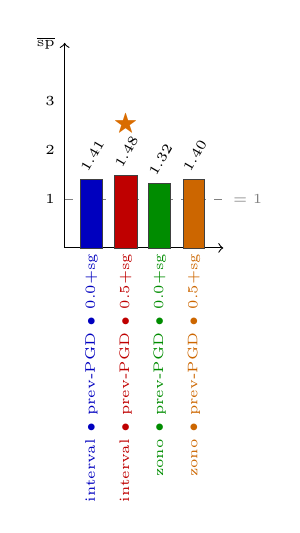
\begin{tikzpicture}[scale=0.62, every node/.style={font=\tiny}]
  \draw[->] (0,0) -- (3.25,0);
  \draw[->] (0,0) -- (0,4.20) node[left]{$\overline{\text{sp}}$};
  \draw[dashed, gray] (0,1) -- (3.25,1) node[right]{$=1$};
  \node[left, font=\tiny] at (0,1) {1};
  \node[left, font=\tiny] at (0,2) {2};
  \node[left, font=\tiny] at (0,3) {3};
  \fill[blue!75!black] (0.33,0) rectangle (0.78,1.405);
  \draw[gray!50!black, line width=0.2pt] (0.33,0) rectangle (0.78,1.405);
  \node[anchor=south west, rotate=60, font=\tiny, inner sep=1pt] at (0.50,1.455) {1.41};
  \node[anchor=east, rotate=90, font=\tiny, text=blue!75!black, inner sep=1pt] at (0.55,-0.05) {interval $\bullet$ prev-PGD $\bullet$ 0.0+sg};
  \fill[red!75!black] (1.02,0) rectangle (1.48,1.485);
  \draw[gray!50!black, line width=0.2pt] (1.02,0) rectangle (1.48,1.485);
  \node[anchor=south west, rotate=60, font=\tiny, inner sep=1pt] at (1.20,1.535) {1.48};
  \node[anchor=east, rotate=90, font=\tiny, text=red!75!black, inner sep=1pt] at (1.25,-0.05) {interval $\bullet$ prev-PGD $\bullet$ 0.5+sg};
  \fill[green!55!black] (1.72,0) rectangle (2.17,1.325);
  \draw[gray!50!black, line width=0.2pt] (1.72,0) rectangle (2.17,1.325);
  \node[anchor=south west, rotate=60, font=\tiny, inner sep=1pt] at (1.90,1.375) {1.32};
  \node[anchor=east, rotate=90, font=\tiny, text=green!55!black, inner sep=1pt] at (1.95,-0.05) {zono $\bullet$ prev-PGD $\bullet$ 0.0+sg};
  \fill[orange!80!black] (2.42,0) rectangle (2.87,1.404);
  \draw[gray!50!black, line width=0.2pt] (2.42,0) rectangle (2.87,1.404);
  \node[anchor=south west, rotate=60, font=\tiny, inner sep=1pt] at (2.60,1.454) {1.40};
  \node[anchor=east, rotate=90, font=\tiny, text=orange!80!black, inner sep=1pt] at (2.65,-0.05) {zono $\bullet$ prev-PGD $\bullet$ 0.5+sg};
  \node[font=\small, text=orange!85!black] at (1.25,2.53) {$\bigstar$};
\end{tikzpicture}
\end{center}
\end{minipage}
\hfill
\begin{minipage}[t]{0.48\linewidth}
\begin{center}
\scriptsize
\colorbox{cyan!30}{\textbf{win}}\;\textbf{ALL} \textbar{} pert \textbf{translation} (p\_sizes merged: \texttt{1,1}, \texttt{3,1}, \texttt{3,3}) \textbar{} 4 combos, total $n=738$ cells, $n_{\max}=202$.\\[0.4ex]
\textbf{Ranking (best $\to$ worst):}\ \textcolor{orange!85!black}{$\bigstar$}\textcolor{red!75!black}{\rule{0.55em}{0.55em}}\,81\%\,(112f+21t/165) ~ \textcolor{orange!80!black}{\rule{0.55em}{0.55em}}\,77\%\,(134f+22t/202) ~ \textcolor{blue!75!black}{\rule{0.55em}{0.55em}}\,74\%\,(106f+21t/172) ~ \textcolor{green!55!black}{\rule{0.55em}{0.55em}}\,72\%\,(121f+23t/199)\\[0.4ex]
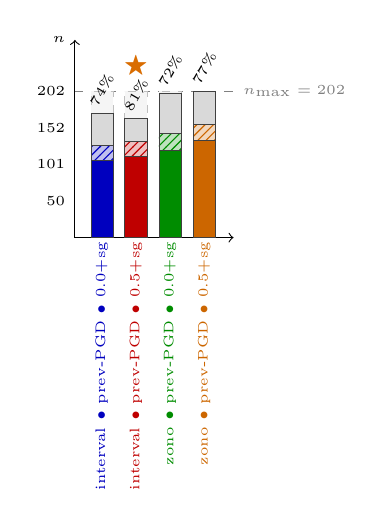
\begin{tikzpicture}[scale=0.62, every node/.style={font=\tiny}]
  \draw[->] (0,0) -- (3.25,0);
  \draw[->] (0,0) -- (0,4.05) node[left]{$n$};
  \draw[dashed, gray] (0,3.00) -- (3.25,3.00) node[right]{$n_{\max}=202$};
  \node[left, font=\tiny] at (0,0.75) {50};
  \node[left, font=\tiny] at (0,1.50) {101};
  \node[left, font=\tiny] at (0,2.25) {152};
  \node[left, font=\tiny] at (0,3.00) {202};
  \fill[gray!8] (0.33,0) rectangle (0.78,3.000);
  \draw[gray!50, line width=0.2pt, dashed] (0.33,0) rectangle (0.78,3.000);
  \fill[gray!30] (0.33,0) rectangle (0.78,2.554);
  \draw[gray!50!black, line width=0.2pt] (0.33,0) rectangle (0.78,2.554);
  \fill[blue!75!black] (0.33,0) rectangle (0.78,1.574);
  \draw[gray!50!black, line width=0.2pt] (0.33,0) rectangle (0.78,1.574);
  \fill[white] (0.33,1.574) rectangle (0.78,1.886);
  \fill[blue!75!black, opacity=0.25] (0.33,1.574) rectangle (0.78,1.886);
  \fill[pattern=north east lines, pattern color=blue!75!black] (0.33,1.574) rectangle (0.78,1.886);
  \draw[gray!50!black, line width=0.2pt] (0.33,1.574) rectangle (0.78,1.886);
  \node[anchor=south west, rotate=60, font=\tiny, inner sep=1pt] at (0.50,2.574) {74\%};
  \node[anchor=east, rotate=90, font=\tiny, text=blue!75!black, inner sep=1pt] at (0.55,-0.02) {interval $\bullet$ prev-PGD $\bullet$ 0.0+sg};
  \fill[gray!8] (1.02,0) rectangle (1.48,3.000);
  \draw[gray!50, line width=0.2pt, dashed] (1.02,0) rectangle (1.48,3.000);
  \fill[gray!30] (1.02,0) rectangle (1.48,2.450);
  \draw[gray!50!black, line width=0.2pt] (1.02,0) rectangle (1.48,2.450);
  \fill[red!75!black] (1.02,0) rectangle (1.48,1.663);
  \draw[gray!50!black, line width=0.2pt] (1.02,0) rectangle (1.48,1.663);
  \fill[white] (1.02,1.663) rectangle (1.48,1.975);
  \fill[red!75!black, opacity=0.25] (1.02,1.663) rectangle (1.48,1.975);
  \fill[pattern=north east lines, pattern color=red!75!black] (1.02,1.663) rectangle (1.48,1.975);
  \draw[gray!50!black, line width=0.2pt] (1.02,1.663) rectangle (1.48,1.975);
  \node[anchor=south west, rotate=60, font=\tiny, inner sep=1pt] at (1.20,2.470) {81\%};
  \node[anchor=east, rotate=90, font=\tiny, text=red!75!black, inner sep=1pt] at (1.25,-0.02) {interval $\bullet$ prev-PGD $\bullet$ 0.5+sg};
  \fill[gray!8] (1.72,0) rectangle (2.17,3.000);
  \draw[gray!50, line width=0.2pt, dashed] (1.72,0) rectangle (2.17,3.000);
  \fill[gray!30] (1.72,0) rectangle (2.17,2.955);
  \draw[gray!50!black, line width=0.2pt] (1.72,0) rectangle (2.17,2.955);
  \fill[green!55!black] (1.72,0) rectangle (2.17,1.797);
  \draw[gray!50!black, line width=0.2pt] (1.72,0) rectangle (2.17,1.797);
  \fill[white] (1.72,1.797) rectangle (2.17,2.139);
  \fill[green!55!black, opacity=0.25] (1.72,1.797) rectangle (2.17,2.139);
  \fill[pattern=north east lines, pattern color=green!55!black] (1.72,1.797) rectangle (2.17,2.139);
  \draw[gray!50!black, line width=0.2pt] (1.72,1.797) rectangle (2.17,2.139);
  \node[anchor=south west, rotate=60, font=\tiny, inner sep=1pt] at (1.90,2.975) {72\%};
  \node[anchor=east, rotate=90, font=\tiny, text=green!55!black, inner sep=1pt] at (1.95,-0.02) {zono $\bullet$ prev-PGD $\bullet$ 0.0+sg};
  \fill[gray!8] (2.42,0) rectangle (2.87,3.000);
  \draw[gray!50, line width=0.2pt, dashed] (2.42,0) rectangle (2.87,3.000);
  \fill[gray!30] (2.42,0) rectangle (2.87,3.000);
  \draw[gray!50!black, line width=0.2pt] (2.42,0) rectangle (2.87,3.000);
  \fill[orange!80!black] (2.42,0) rectangle (2.87,1.990);
  \draw[gray!50!black, line width=0.2pt] (2.42,0) rectangle (2.87,1.990);
  \fill[white] (2.42,1.990) rectangle (2.87,2.317);
  \fill[orange!80!black, opacity=0.25] (2.42,1.990) rectangle (2.87,2.317);
  \fill[pattern=north east lines, pattern color=orange!80!black] (2.42,1.990) rectangle (2.87,2.317);
  \draw[gray!50!black, line width=0.2pt] (2.42,1.990) rectangle (2.87,2.317);
  \node[anchor=south west, rotate=60, font=\tiny, inner sep=1pt] at (2.60,3.020) {77\%};
  \node[anchor=east, rotate=90, font=\tiny, text=orange!80!black, inner sep=1pt] at (2.65,-0.02) {zono $\bullet$ prev-PGD $\bullet$ 0.5+sg};
  \node[font=\small, text=orange!85!black] at (1.25,3.50) {$\bigstar$};
\end{tikzpicture}
\end{center}
\end{minipage}

\par\medskip\noindent
\begin{minipage}[t]{0.48\linewidth}
\begin{center}
\scriptsize
\colorbox{yellow!40}{\textbf{sp}}\;\textbf{ALL} \textbar{} pert \textbf{linf} (p\_sizes merged: \texttt{0.1}) \textbar{} 4 combos, total $n=217$ cells.\\[0.4ex]
\textbf{Ranking (best $\to$ worst):}\ \textcolor{orange!85!black}{$\bigstar$}\textcolor{blue!75!black}{\rule{0.55em}{0.55em}}\,1.06\,(1/1) ~ \textcolor{red!75!black}{\rule{0.55em}{0.55em}}\,1.05\,(1/1) ~ \textcolor{green!55!black}{\rule{0.55em}{0.55em}}\,1.03\,(1/1) ~ \textcolor{orange!80!black}{\rule{0.55em}{0.55em}}\,0.99\,(1/1)\\[0.4ex]
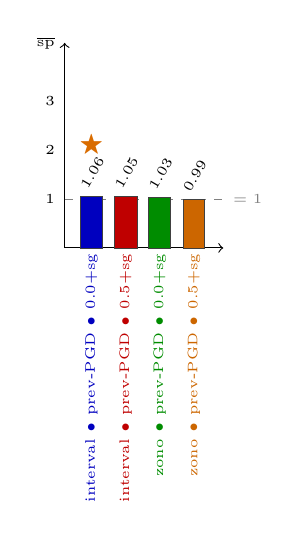
\begin{tikzpicture}[scale=0.62, every node/.style={font=\tiny}]
  \draw[->] (0,0) -- (3.25,0);
  \draw[->] (0,0) -- (0,4.20) node[left]{$\overline{\text{sp}}$};
  \draw[dashed, gray] (0,1) -- (3.25,1) node[right]{$=1$};
  \node[left, font=\tiny] at (0,1) {1};
  \node[left, font=\tiny] at (0,2) {2};
  \node[left, font=\tiny] at (0,3) {3};
  \fill[blue!75!black] (0.33,0) rectangle (0.78,1.060);
  \draw[gray!50!black, line width=0.2pt] (0.33,0) rectangle (0.78,1.060);
  \node[anchor=south west, rotate=60, font=\tiny, inner sep=1pt] at (0.50,1.110) {1.06};
  \node[anchor=east, rotate=90, font=\tiny, text=blue!75!black, inner sep=1pt] at (0.55,-0.05) {interval $\bullet$ prev-PGD $\bullet$ 0.0+sg};
  \fill[red!75!black] (1.02,0) rectangle (1.48,1.052);
  \draw[gray!50!black, line width=0.2pt] (1.02,0) rectangle (1.48,1.052);
  \node[anchor=south west, rotate=60, font=\tiny, inner sep=1pt] at (1.20,1.102) {1.05};
  \node[anchor=east, rotate=90, font=\tiny, text=red!75!black, inner sep=1pt] at (1.25,-0.05) {interval $\bullet$ prev-PGD $\bullet$ 0.5+sg};
  \fill[green!55!black] (1.72,0) rectangle (2.17,1.031);
  \draw[gray!50!black, line width=0.2pt] (1.72,0) rectangle (2.17,1.031);
  \node[anchor=south west, rotate=60, font=\tiny, inner sep=1pt] at (1.90,1.081) {1.03};
  \node[anchor=east, rotate=90, font=\tiny, text=green!55!black, inner sep=1pt] at (1.95,-0.05) {zono $\bullet$ prev-PGD $\bullet$ 0.0+sg};
  \fill[orange!80!black] (2.42,0) rectangle (2.87,0.992);
  \draw[gray!50!black, line width=0.2pt] (2.42,0) rectangle (2.87,0.992);
  \node[anchor=south west, rotate=60, font=\tiny, inner sep=1pt] at (2.60,1.042) {0.99};
  \node[anchor=east, rotate=90, font=\tiny, text=orange!80!black, inner sep=1pt] at (2.65,-0.05) {zono $\bullet$ prev-PGD $\bullet$ 0.5+sg};
  \node[font=\small, text=orange!85!black] at (0.55,2.11) {$\bigstar$};
\end{tikzpicture}
\end{center}
\end{minipage}
\hfill
\begin{minipage}[t]{0.48\linewidth}
\begin{center}
\scriptsize
\colorbox{cyan!30}{\textbf{win}}\;\textbf{ALL} \textbar{} pert \textbf{linf} (p\_sizes merged: \texttt{0.1}) \textbar{} 4 combos, total $n=217$ cells, $n_{\max}=60$.\\[0.4ex]
\textbf{Ranking (best $\to$ worst):}\ \textcolor{orange!85!black}{$\bigstar$}\textcolor{red!75!black}{\rule{0.55em}{0.55em}}\,80\%\,(11f+29t/50) ~ \textcolor{orange!80!black}{\rule{0.55em}{0.55em}}\,72\%\,(12f+31t/60) ~ \textcolor{blue!75!black}{\rule{0.55em}{0.55em}}\,71\%\,(11f+24t/49) ~ \textcolor{green!55!black}{\rule{0.55em}{0.55em}}\,62\%\,(15f+21t/58)\\[0.4ex]
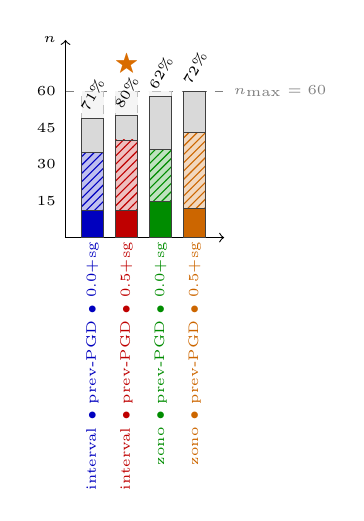
\begin{tikzpicture}[scale=0.62, every node/.style={font=\tiny}]
  \draw[->] (0,0) -- (3.25,0);
  \draw[->] (0,0) -- (0,4.05) node[left]{$n$};
  \draw[dashed, gray] (0,3.00) -- (3.25,3.00) node[right]{$n_{\max}=60$};
  \node[left, font=\tiny] at (0,0.75) {15};
  \node[left, font=\tiny] at (0,1.50) {30};
  \node[left, font=\tiny] at (0,2.25) {45};
  \node[left, font=\tiny] at (0,3.00) {60};
  \fill[gray!8] (0.33,0) rectangle (0.78,3.000);
  \draw[gray!50, line width=0.2pt, dashed] (0.33,0) rectangle (0.78,3.000);
  \fill[gray!30] (0.33,0) rectangle (0.78,2.450);
  \draw[gray!50!black, line width=0.2pt] (0.33,0) rectangle (0.78,2.450);
  \fill[blue!75!black] (0.33,0) rectangle (0.78,0.550);
  \draw[gray!50!black, line width=0.2pt] (0.33,0) rectangle (0.78,0.550);
  \fill[white] (0.33,0.550) rectangle (0.78,1.750);
  \fill[blue!75!black, opacity=0.25] (0.33,0.550) rectangle (0.78,1.750);
  \fill[pattern=north east lines, pattern color=blue!75!black] (0.33,0.550) rectangle (0.78,1.750);
  \draw[gray!50!black, line width=0.2pt] (0.33,0.550) rectangle (0.78,1.750);
  \node[anchor=south west, rotate=60, font=\tiny, inner sep=1pt] at (0.50,2.470) {71\%};
  \node[anchor=east, rotate=90, font=\tiny, text=blue!75!black, inner sep=1pt] at (0.55,-0.02) {interval $\bullet$ prev-PGD $\bullet$ 0.0+sg};
  \fill[gray!8] (1.02,0) rectangle (1.48,3.000);
  \draw[gray!50, line width=0.2pt, dashed] (1.02,0) rectangle (1.48,3.000);
  \fill[gray!30] (1.02,0) rectangle (1.48,2.500);
  \draw[gray!50!black, line width=0.2pt] (1.02,0) rectangle (1.48,2.500);
  \fill[red!75!black] (1.02,0) rectangle (1.48,0.550);
  \draw[gray!50!black, line width=0.2pt] (1.02,0) rectangle (1.48,0.550);
  \fill[white] (1.02,0.550) rectangle (1.48,2.000);
  \fill[red!75!black, opacity=0.25] (1.02,0.550) rectangle (1.48,2.000);
  \fill[pattern=north east lines, pattern color=red!75!black] (1.02,0.550) rectangle (1.48,2.000);
  \draw[gray!50!black, line width=0.2pt] (1.02,0.550) rectangle (1.48,2.000);
  \node[anchor=south west, rotate=60, font=\tiny, inner sep=1pt] at (1.20,2.520) {80\%};
  \node[anchor=east, rotate=90, font=\tiny, text=red!75!black, inner sep=1pt] at (1.25,-0.02) {interval $\bullet$ prev-PGD $\bullet$ 0.5+sg};
  \fill[gray!8] (1.72,0) rectangle (2.17,3.000);
  \draw[gray!50, line width=0.2pt, dashed] (1.72,0) rectangle (2.17,3.000);
  \fill[gray!30] (1.72,0) rectangle (2.17,2.900);
  \draw[gray!50!black, line width=0.2pt] (1.72,0) rectangle (2.17,2.900);
  \fill[green!55!black] (1.72,0) rectangle (2.17,0.750);
  \draw[gray!50!black, line width=0.2pt] (1.72,0) rectangle (2.17,0.750);
  \fill[white] (1.72,0.750) rectangle (2.17,1.800);
  \fill[green!55!black, opacity=0.25] (1.72,0.750) rectangle (2.17,1.800);
  \fill[pattern=north east lines, pattern color=green!55!black] (1.72,0.750) rectangle (2.17,1.800);
  \draw[gray!50!black, line width=0.2pt] (1.72,0.750) rectangle (2.17,1.800);
  \node[anchor=south west, rotate=60, font=\tiny, inner sep=1pt] at (1.90,2.920) {62\%};
  \node[anchor=east, rotate=90, font=\tiny, text=green!55!black, inner sep=1pt] at (1.95,-0.02) {zono $\bullet$ prev-PGD $\bullet$ 0.0+sg};
  \fill[gray!8] (2.42,0) rectangle (2.87,3.000);
  \draw[gray!50, line width=0.2pt, dashed] (2.42,0) rectangle (2.87,3.000);
  \fill[gray!30] (2.42,0) rectangle (2.87,3.000);
  \draw[gray!50!black, line width=0.2pt] (2.42,0) rectangle (2.87,3.000);
  \fill[orange!80!black] (2.42,0) rectangle (2.87,0.600);
  \draw[gray!50!black, line width=0.2pt] (2.42,0) rectangle (2.87,0.600);
  \fill[white] (2.42,0.600) rectangle (2.87,2.150);
  \fill[orange!80!black, opacity=0.25] (2.42,0.600) rectangle (2.87,2.150);
  \fill[pattern=north east lines, pattern color=orange!80!black] (2.42,0.600) rectangle (2.87,2.150);
  \draw[gray!50!black, line width=0.2pt] (2.42,0.600) rectangle (2.87,2.150);
  \node[anchor=south west, rotate=60, font=\tiny, inner sep=1pt] at (2.60,3.020) {72\%};
  \node[anchor=east, rotate=90, font=\tiny, text=orange!80!black, inner sep=1pt] at (2.65,-0.02) {zono $\bullet$ prev-PGD $\bullet$ 0.5+sg};
  \node[font=\small, text=orange!85!black] at (1.25,3.55) {$\bigstar$};
\end{tikzpicture}
\end{center}
\end{minipage}

\clearpage
\section*{Overall histograms across all architectures and perturbations: $\overline{\text{sp}}$ paired with win-rate}
This section pools every $(c_\mathrm{src}, c_\mathrm{tgt}, \text{seed})$ cell across \emph{all} architectures \emph{and} \emph{all} perturbation types into a single paired row — one bar per combo summarising every cell on record. Bar definitions are the same as in the sections above; both the architecture and the perturbation are shown as \textbf{ALL} in each chart's caption.
\noindent\textbf{Note:} these histograms are restricted to the 4 combinations \texttt{zono:prev\_pgd:0.0+sg}, \texttt{zono:prev\_pgd:0.5+sg}, \texttt{interval:prev\_pgd:0.0+sg}, \texttt{interval:prev\_pgd:0.5+sg} (via \texttt{--combination\_table}).
\par\medskip\noindent
\begin{minipage}[t]{0.48\linewidth}
\begin{center}
\scriptsize
\colorbox{yellow!40}{\textbf{sp}}\;\textbf{ALL} \textbar{} pert \textbf{ALL} (p\_sizes merged: \texttt{0.1}, \texttt{1,1}, \texttt{1,14,14,3}, \texttt{3,1}, \texttt{3,3}, \texttt{3,3,5}, \texttt{5,5,5}) \textbar{} 4 combos, total $n=1700$ cells.\\[0.4ex]
\textbf{Ranking (best $\to$ worst):}\ \textcolor{orange!85!black}{$\bigstar$}\textcolor{red!75!black}{\rule{0.55em}{0.55em}}\,1.38\,(7/7) ~ \textcolor{blue!75!black}{\rule{0.55em}{0.55em}}\,1.34\,(7/7) ~ \textcolor{orange!80!black}{\rule{0.55em}{0.55em}}\,1.33\,(7/7) ~ \textcolor{green!55!black}{\rule{0.55em}{0.55em}}\,1.27\,(7/7)\\[0.4ex]
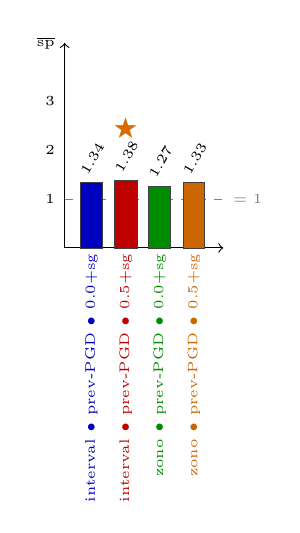
\begin{tikzpicture}[scale=0.62, every node/.style={font=\tiny}]
  \draw[->] (0,0) -- (3.25,0);
  \draw[->] (0,0) -- (0,4.20) node[left]{$\overline{\text{sp}}$};
  \draw[dashed, gray] (0,1) -- (3.25,1) node[right]{$=1$};
  \node[left, font=\tiny] at (0,1) {1};
  \node[left, font=\tiny] at (0,2) {2};
  \node[left, font=\tiny] at (0,3) {3};
  \fill[blue!75!black] (0.33,0) rectangle (0.78,1.337);
  \draw[gray!50!black, line width=0.2pt] (0.33,0) rectangle (0.78,1.337);
  \node[anchor=south west, rotate=60, font=\tiny, inner sep=1pt] at (0.50,1.387) {1.34};
  \node[anchor=east, rotate=90, font=\tiny, text=blue!75!black, inner sep=1pt] at (0.55,-0.05) {interval $\bullet$ prev-PGD $\bullet$ 0.0+sg};
  \fill[red!75!black] (1.02,0) rectangle (1.48,1.380);
  \draw[gray!50!black, line width=0.2pt] (1.02,0) rectangle (1.48,1.380);
  \node[anchor=south west, rotate=60, font=\tiny, inner sep=1pt] at (1.20,1.430) {1.38};
  \node[anchor=east, rotate=90, font=\tiny, text=red!75!black, inner sep=1pt] at (1.25,-0.05) {interval $\bullet$ prev-PGD $\bullet$ 0.5+sg};
  \fill[green!55!black] (1.72,0) rectangle (2.17,1.273);
  \draw[gray!50!black, line width=0.2pt] (1.72,0) rectangle (2.17,1.273);
  \node[anchor=south west, rotate=60, font=\tiny, inner sep=1pt] at (1.90,1.323) {1.27};
  \node[anchor=east, rotate=90, font=\tiny, text=green!55!black, inner sep=1pt] at (1.95,-0.05) {zono $\bullet$ prev-PGD $\bullet$ 0.0+sg};
  \fill[orange!80!black] (2.42,0) rectangle (2.87,1.335);
  \draw[gray!50!black, line width=0.2pt] (2.42,0) rectangle (2.87,1.335);
  \node[anchor=south west, rotate=60, font=\tiny, inner sep=1pt] at (2.60,1.385) {1.33};
  \node[anchor=east, rotate=90, font=\tiny, text=orange!80!black, inner sep=1pt] at (2.65,-0.05) {zono $\bullet$ prev-PGD $\bullet$ 0.5+sg};
  \node[font=\small, text=orange!85!black] at (1.25,2.43) {$\bigstar$};
\end{tikzpicture}
\end{center}
\end{minipage}
\hfill
\begin{minipage}[t]{0.48\linewidth}
\begin{center}
\scriptsize
\colorbox{cyan!30}{\textbf{win}}\;\textbf{ALL} \textbar{} pert \textbf{ALL} (p\_sizes merged: \texttt{0.1}, \texttt{1,1}, \texttt{1,14,14,3}, \texttt{3,1}, \texttt{3,3}, \texttt{3,3,5}, \texttt{5,5,5}) \textbar{} 4 combos, total $n=1700$ cells, $n_{\max}=463$.\\[0.4ex]
\textbf{Ranking (best $\to$ worst):}\ \textcolor{orange!85!black}{$\bigstar$}\textcolor{red!75!black}{\rule{0.55em}{0.55em}}\,79\%\,(203f+101t/386) ~ \textcolor{orange!80!black}{\rule{0.55em}{0.55em}}\,76\%\,(246f+104t/460) ~ \textcolor{blue!75!black}{\rule{0.55em}{0.55em}}\,70\%\,(188f+85t/391) ~ \textcolor{green!55!black}{\rule{0.55em}{0.55em}}\,67\%\,(229f+79t/463)\\[0.4ex]
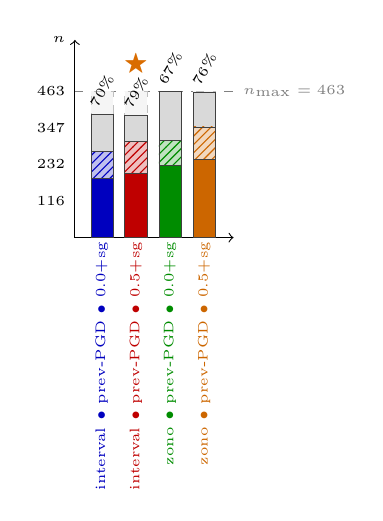
\begin{tikzpicture}[scale=0.62, every node/.style={font=\tiny}]
  \draw[->] (0,0) -- (3.25,0);
  \draw[->] (0,0) -- (0,4.05) node[left]{$n$};
  \draw[dashed, gray] (0,3.00) -- (3.25,3.00) node[right]{$n_{\max}=463$};
  \node[left, font=\tiny] at (0,0.75) {116};
  \node[left, font=\tiny] at (0,1.50) {232};
  \node[left, font=\tiny] at (0,2.25) {347};
  \node[left, font=\tiny] at (0,3.00) {463};
  \fill[gray!8] (0.33,0) rectangle (0.78,3.000);
  \draw[gray!50, line width=0.2pt, dashed] (0.33,0) rectangle (0.78,3.000);
  \fill[gray!30] (0.33,0) rectangle (0.78,2.533);
  \draw[gray!50!black, line width=0.2pt] (0.33,0) rectangle (0.78,2.533);
  \fill[blue!75!black] (0.33,0) rectangle (0.78,1.218);
  \draw[gray!50!black, line width=0.2pt] (0.33,0) rectangle (0.78,1.218);
  \fill[white] (0.33,1.218) rectangle (0.78,1.769);
  \fill[blue!75!black, opacity=0.25] (0.33,1.218) rectangle (0.78,1.769);
  \fill[pattern=north east lines, pattern color=blue!75!black] (0.33,1.218) rectangle (0.78,1.769);
  \draw[gray!50!black, line width=0.2pt] (0.33,1.218) rectangle (0.78,1.769);
  \node[anchor=south west, rotate=60, font=\tiny, inner sep=1pt] at (0.50,2.553) {70\%};
  \node[anchor=east, rotate=90, font=\tiny, text=blue!75!black, inner sep=1pt] at (0.55,-0.02) {interval $\bullet$ prev-PGD $\bullet$ 0.0+sg};
  \fill[gray!8] (1.02,0) rectangle (1.48,3.000);
  \draw[gray!50, line width=0.2pt, dashed] (1.02,0) rectangle (1.48,3.000);
  \fill[gray!30] (1.02,0) rectangle (1.48,2.501);
  \draw[gray!50!black, line width=0.2pt] (1.02,0) rectangle (1.48,2.501);
  \fill[red!75!black] (1.02,0) rectangle (1.48,1.315);
  \draw[gray!50!black, line width=0.2pt] (1.02,0) rectangle (1.48,1.315);
  \fill[white] (1.02,1.315) rectangle (1.48,1.970);
  \fill[red!75!black, opacity=0.25] (1.02,1.315) rectangle (1.48,1.970);
  \fill[pattern=north east lines, pattern color=red!75!black] (1.02,1.315) rectangle (1.48,1.970);
  \draw[gray!50!black, line width=0.2pt] (1.02,1.315) rectangle (1.48,1.970);
  \node[anchor=south west, rotate=60, font=\tiny, inner sep=1pt] at (1.20,2.521) {79\%};
  \node[anchor=east, rotate=90, font=\tiny, text=red!75!black, inner sep=1pt] at (1.25,-0.02) {interval $\bullet$ prev-PGD $\bullet$ 0.5+sg};
  \fill[gray!8] (1.72,0) rectangle (2.17,3.000);
  \draw[gray!50, line width=0.2pt, dashed] (1.72,0) rectangle (2.17,3.000);
  \fill[gray!30] (1.72,0) rectangle (2.17,3.000);
  \draw[gray!50!black, line width=0.2pt] (1.72,0) rectangle (2.17,3.000);
  \fill[green!55!black] (1.72,0) rectangle (2.17,1.484);
  \draw[gray!50!black, line width=0.2pt] (1.72,0) rectangle (2.17,1.484);
  \fill[white] (1.72,1.484) rectangle (2.17,1.996);
  \fill[green!55!black, opacity=0.25] (1.72,1.484) rectangle (2.17,1.996);
  \fill[pattern=north east lines, pattern color=green!55!black] (1.72,1.484) rectangle (2.17,1.996);
  \draw[gray!50!black, line width=0.2pt] (1.72,1.484) rectangle (2.17,1.996);
  \node[anchor=south west, rotate=60, font=\tiny, inner sep=1pt] at (1.90,3.020) {67\%};
  \node[anchor=east, rotate=90, font=\tiny, text=green!55!black, inner sep=1pt] at (1.95,-0.02) {zono $\bullet$ prev-PGD $\bullet$ 0.0+sg};
  \fill[gray!8] (2.42,0) rectangle (2.87,3.000);
  \draw[gray!50, line width=0.2pt, dashed] (2.42,0) rectangle (2.87,3.000);
  \fill[gray!30] (2.42,0) rectangle (2.87,2.981);
  \draw[gray!50!black, line width=0.2pt] (2.42,0) rectangle (2.87,2.981);
  \fill[orange!80!black] (2.42,0) rectangle (2.87,1.594);
  \draw[gray!50!black, line width=0.2pt] (2.42,0) rectangle (2.87,1.594);
  \fill[white] (2.42,1.594) rectangle (2.87,2.268);
  \fill[orange!80!black, opacity=0.25] (2.42,1.594) rectangle (2.87,2.268);
  \fill[pattern=north east lines, pattern color=orange!80!black] (2.42,1.594) rectangle (2.87,2.268);
  \draw[gray!50!black, line width=0.2pt] (2.42,1.594) rectangle (2.87,2.268);
  \node[anchor=south west, rotate=60, font=\tiny, inner sep=1pt] at (2.60,3.001) {76\%};
  \node[anchor=east, rotate=90, font=\tiny, text=orange!80!black, inner sep=1pt] at (2.65,-0.02) {zono $\bullet$ prev-PGD $\bullet$ 0.5+sg};
  \node[font=\small, text=orange!85!black] at (1.25,3.55) {$\bigstar$};
\end{tikzpicture}
\end{center}
\end{minipage}

\begin{table}[!htbp]
\centering
\scriptsize
\setlength{\tabcolsep}{4pt}
\begin{adjustbox}{max width=\textwidth,center}%
\begin{tabular}{@{}l l l l l | r r r r r r r r@{}}
\hline
p\_type & p\_size & \tech{bound\_tight} & \tech{varHint} & $\tau$ & c\_src & c\_tgt & n\_relax & t\_std & t\_adv & $\text{sp}$ & $\overline{\text{sp}}_{c\_\mathrm{src}}$ & $\overline{|\delta_\mathrm{std}-\delta_\mathrm{adv}|}_{c\_\mathrm{src}}$ \\
\hline
\rowcolor{green!15} patch       & \texttt{1,14,14,3}   & interval    & prev\_pgd & 0.5+sg &     0 &     1 &   164 &   81.52 &   60.37 & \textbf{1.350} & \textit{\textbf{1.359}} & \textit{0.02} \\
\rowcolor{green!15}             &                      &             &     &      &     0 &     2 &   164 &   45.49 &   33.13 & \textbf{1.373} &         &         \\
\rowcolor{green!15}             &                      &             &     &      &     0 &     3 &   164 &   96.17 &   55.77 & \textbf{1.724} &         &         \\
\rowcolor{green!15}             &                      &             &     &      &     0 &     4 &   164 &  328.21 &  175.30 & \textbf{1.872} &         &         \\
\rowcolor{green!15}             &                      &             &     &      &     0 &     5 &   164 &   62.33 &   40.12 & \textbf{1.554} &         &         \\
\rowcolor{green!15}             &                      &             &     &      &     0 &     6 &   164 &   34.38 &   27.43 & \textbf{1.253} &         &         \\
\rowcolor{green!15}             &                      &             &     &      &     0 &     7 &   164 &   71.72 &  121.01 & 0.593 &         &         \\
\rowcolor{green!15}             &                      &             &     &      &     0 &     8 &   164 &   55.30 &   51.07 & \textbf{1.083} &         &         \\
\rowcolor{green!15}             &                      &             &     &      &     0 &     9 &   164 &   65.33 &   54.39 & \textbf{1.201} &         &         \\
\hline
\rowcolor{green!15}             &                      & interval    & prev\_pgd & 0.0+sg &     0 &     1 &     0 &   81.52 &   44.35 & \textbf{1.838} & \textit{\textbf{1.136}} & \textit{0.03} \\
\rowcolor{green!15}             &                      &             &     &      &     0 &     2 &     0 &   45.49 &   29.94 & \textbf{1.519} &         &         \\
\rowcolor{green!15}             &                      &             &     &      &     0 &     3 &     0 &   96.17 &   44.34 & \textbf{2.169} &         &         \\
\rowcolor{green!15}             &                      &             &     &      &     0 &     4 &     0 &  328.21 &  323.13 & \textbf{1.016} &         &         \\
\rowcolor{green!15}             &                      &             &     &      &     0 &     5 &     0 &   62.33 &   56.11 & \textbf{1.111} &         &         \\
\rowcolor{green!15}             &                      &             &     &      &     0 &     6 &     0 &   34.38 &   49.68 & 0.692 &         &         \\
\rowcolor{green!15}             &                      &             &     &      &     0 &     7 &     0 &   71.72 &   72.22 & 0.993 &         &         \\
\rowcolor{green!15}             &                      &             &     &      &     0 &     8 &     0 &   55.30 &   49.69 & \textbf{1.113} &         &         \\
\rowcolor{green!15}             &                      &             &     &      &     0 &     9 &     0 &   65.33 &   70.60 & 0.925 &         &         \\
\hline
\rowcolor{green!15}             &                      & zono        & prev\_pgd & 0.5+sg &     0 &     1 &   164 &   81.52 &   65.97 & \textbf{1.236} & \textit{\textbf{1.283}} & \textit{0.02} \\
\rowcolor{green!15}             &                      &             &     &      &     0 &     2 &   164 &   45.49 &   36.31 & \textbf{1.253} &         &         \\
\rowcolor{green!15}             &                      &             &     &      &     0 &     3 &   164 &   96.17 &   56.34 & \textbf{1.707} &         &         \\
\rowcolor{green!15}             &                      &             &     &      &     0 &     4 &   164 &  328.21 &  182.41 & \textbf{1.799} &         &         \\
\rowcolor{green!15}             &                      &             &     &      &     0 &     5 &   164 &   62.33 &   39.28 & \textbf{1.587} &         &         \\
\rowcolor{green!15}             &                      &             &     &      &     0 &     6 &   164 &   34.38 &   28.45 & \textbf{1.208} &         &         \\
\rowcolor{green!15}             &                      &             &     &      &     0 &     7 &   164 &   71.72 &  125.19 & 0.573 &         &         \\
\rowcolor{green!15}             &                      &             &     &      &     0 &     8 &   164 &   55.30 &   54.00 & \textbf{1.024} &         &         \\
\rowcolor{green!15}             &                      &             &     &      &     0 &     9 &   164 &   65.33 &   67.28 & 0.971 &         &         \\
\hline
\rowcolor{green!15}             &                      & zono        & prev\_pgd & 0.0+sg &     0 &     1 &     0 &   81.52 &   43.94 & \textbf{1.855} & \textit{\textbf{1.152}} & \textit{0.03} \\
\rowcolor{green!15}             &                      &             &     &      &     0 &     2 &     0 &   45.49 &   38.96 & \textbf{1.168} &         &         \\
\rowcolor{green!15}             &                      &             &     &      &     0 &     3 &     0 &   96.17 &   46.80 & \textbf{2.055} &         &         \\
\rowcolor{green!15}             &                      &             &     &      &     0 &     4 &     0 &  328.21 &  288.53 & \textbf{1.138} &         &         \\
\rowcolor{green!15}             &                      &             &     &      &     0 &     5 &     0 &   62.33 &   57.72 & \textbf{1.080} &         &         \\
\rowcolor{green!15}             &                      &             &     &      &     0 &     6 &     0 &   34.38 &   54.04 & 0.636 &         &         \\
\rowcolor{green!15}             &                      &             &     &      &     0 &     7 &     0 &   71.72 &   77.27 & 0.928 &         &         \\
\rowcolor{green!15}             &                      &             &     &      &     0 &     8 &     0 &   55.30 &   51.10 & \textbf{1.082} &         &         \\
\rowcolor{green!15}             &                      &             &     &      &     0 &     9 &     0 &   65.33 &   71.03 & 0.920 &         &         \\
\hline
\rowcolor{yellow!25}             &                      & interval    & prev\_pgd & 0.5+sg &     1 &     0 &   164 &   56.34 &   63.35 & 0.889 & \textit{\textbf{1.942}} & \textit{0.02} \\
\rowcolor{yellow!25}             &                      &             &     &      &     1 &     2 &   164 &   54.24 &   54.18 & \textbf{1.001} &         &         \\
\rowcolor{yellow!25}             &                      &             &     &      &     1 &     3 &   164 &   94.60 &   22.92 & \textbf{4.127} &         &         \\
\rowcolor{yellow!25}             &                      &             &     &      &     1 &     4 &   164 &  113.19 &   67.25 & \textbf{1.683} &         &         \\
\rowcolor{yellow!25}             &                      &             &     &      &     1 &     5 &   164 &  138.25 &   40.35 & \textbf{3.426} &         &         \\
\rowcolor{yellow!25}             &                      &             &     &      &     1 &     6 &   164 &  206.61 &  140.19 & \textbf{1.474} &         &         \\
\rowcolor{yellow!25}             &                      &             &     &      &     1 &     7 &   164 &   83.24 &   35.05 & \textbf{2.375} &         &         \\
\rowcolor{yellow!25}             &                      &             &     &      &     1 &     8 &   164 &   67.32 &   20.62 & \textbf{3.265} &         &         \\
\rowcolor{yellow!25}             &                      &             &     &      &     1 &     9 &   164 &  102.50 &   27.92 & \textbf{3.671} &         &         \\
\hline
\rowcolor{yellow!25}             &                      & zono        & prev\_pgd & 0.5+sg &     1 &     0 &   164 &   56.34 &   46.50 & \textbf{1.212} & \textit{\textbf{2.025}} & \textit{0.02} \\
\rowcolor{yellow!25}             &                      &             &     &      &     1 &     2 &   164 &   54.24 &   36.01 & \textbf{1.506} &         &         \\
\rowcolor{yellow!25}             &                      &             &     &      &     1 &     3 &   164 &   94.60 &   26.15 & \textbf{3.618} &         &         \\
\rowcolor{yellow!25}             &                      &             &     &      &     1 &     4 &   164 &  113.19 &   49.23 & \textbf{2.299} &         &         \\
\rowcolor{yellow!25}             &                      &             &     &      &     1 &     5 &   164 &  138.25 &   67.20 & \textbf{2.057} &         &         \\
\rowcolor{yellow!25}             &                      &             &     &      &     1 &     6 &   164 &  206.61 &  122.51 & \textbf{1.686} &         &         \\
\rowcolor{yellow!25}             &                      &             &     &      &     1 &     7 &   164 &   83.24 &   33.22 & \textbf{2.506} &         &         \\
\rowcolor{yellow!25}             &                      &             &     &      &     1 &     8 &   164 &   67.32 &   44.88 & \textbf{1.500} &         &         \\
\rowcolor{yellow!25}             &                      &             &     &      &     1 &     9 &   164 &  102.50 &   26.89 & \textbf{3.812} &         &         \\
\hline
\rowcolor{yellow!25}             &                      & interval    & prev\_pgd & 0.0+sg &     1 &     0 &     0 &   56.34 &   39.82 & \textbf{1.415} & \textit{\textbf{1.281}} & \textit{0.02} \\
\rowcolor{yellow!25}             &                      &             &     &      &     1 &     2 &     0 &   54.24 &  127.86 & 0.424 &         &         \\
\rowcolor{yellow!25}             &                      &             &     &      &     1 &     3 &     0 &   94.60 &   24.81 & \textbf{3.813} &         &         \\
\rowcolor{yellow!25}             &                      &             &     &      &     1 &     4 &     0 &  113.19 &   69.83 & \textbf{1.621} &         &         \\
\rowcolor{yellow!25}             &                      &             &     &      &     1 &     5 &     0 &  138.25 &   82.29 & \textbf{1.680} &         &         \\
\rowcolor{yellow!25}             &                      &             &     &      &     1 &     6 &     0 &  206.61 &  138.34 & \textbf{1.493} &         &         \\
\rowcolor{yellow!25}             &                      &             &     &      &     1 &     7 &     0 &   83.24 &  100.81 & 0.826 &         &         \\
\rowcolor{yellow!25}             &                      &             &     &      &     1 &     8 &     0 &   67.32 &   43.19 & \textbf{1.559} &         &         \\
\rowcolor{yellow!25}             &                      &             &     &      &     1 &     9 &     0 &  102.50 &   88.31 & \textbf{1.161} &         &         \\
\hline
\rowcolor{yellow!25}             &                      & zono        & prev\_pgd & 0.0+sg &     1 &     0 &     0 &   56.34 &   41.71 & \textbf{1.351} & \textit{0.282} & \textit{0.02} \\
\rowcolor{yellow!25}             &                      &             &     &      &     1 &     2 &     0 &   54.24 &   66.38 & 0.817 &         &         \\
\rowcolor{yellow!25}             &                      &             &     &      &     1 &     3 &     0 &   94.60 &   49.35 & \textbf{1.917} &         &         \\
\rowcolor{yellow!25}             &                      &             &     &      &     1 &     4 &     0 &  113.19 &   45.67 & \textbf{2.478} &         &         \\
\rowcolor{yellow!25}             &                      &             &     &      &     1 &     5 &     0 &  138.25 &   48.83 & \textbf{2.831} &         &         \\
\rowcolor{yellow!25}             &                      &             &     &      &     1 &     6 &     0 &  206.61 & 2654.58 & 0.078 &         &         \\
\rowcolor{yellow!25}             &                      &             &     &      &     1 &     7 &     0 &   83.24 &  189.58 & 0.439 &         &         \\
\rowcolor{yellow!25}             &                      &             &     &      &     1 &     8 &     0 &   67.32 &   60.46 & \textbf{1.113} &         &         \\
\rowcolor{yellow!25}             &                      &             &     &      &     1 &     9 &     0 &  102.50 &   87.14 & \textbf{1.176} &         &         \\
\hline
\rowcolor{magenta!20}             &                      & zono        & prev\_pgd & 0.5+sg &     2 &     0 &   164 &   79.56 &   36.21 & \textbf{2.197} & \textit{\textbf{3.441}} & \textit{0.83} \\
\rowcolor{magenta!20}             &                      &             &     &      &     2 &     1 &   164 &   95.11 &   78.98 & \textbf{1.204} &         &         \\
\rowcolor{magenta!20}             &                      &             &     &      &     2 &     3 &   164 &  129.59 &   60.25 & \textbf{2.151} &         &         \\
\rowcolor{magenta!20}             &                      &             &     &      &     2 &     4 &   164 &  130.79 &  155.45 & 0.841 &         &         \\
\rowcolor{magenta!20}             &                      &             &     &      &     2 &     5 &   164 &  161.86 &  141.80 & \textbf{1.141} &         &         \\
\rowcolor{magenta!20}             &                      &             &     &      &     2 &     6 &   164 & 1819.45 &  153.59 & \textbf{11.846} &         &         \\
\rowcolor{magenta!20}             &                      &             &     &      &     2 &     7 &   164 &  369.96 &   82.80 & \textbf{4.468} &         &         \\
\rowcolor{magenta!20}             &                      &             &     &      &     2 &     8 &   164 &   88.80 &   88.15 & \textbf{1.007} &         &         \\
\rowcolor{magenta!20}             &                      &             &     &      &     2 &     9 &   164 &   71.08 &   59.09 & \textbf{1.203} &         &         \\
\hline
\rowcolor{magenta!20}             &                      & zono        & prev\_pgd & 0.0+sg &     2 &     0 &     0 &   79.56 &   44.07 & \textbf{1.805} & \textit{\textbf{2.413}} & \textit{0.83} \\
\rowcolor{magenta!20}             &                      &             &     &      &     2 &     1 &     0 &   95.11 &  225.68 & 0.421 &         &         \\
\rowcolor{magenta!20}             &                      &             &     &      &     2 &     3 &     0 &  129.59 &   30.28 & \textbf{4.280} &         &         \\
\rowcolor{magenta!20}             &                      &             &     &      &     2 &     4 &     0 &  130.79 &  152.97 & 0.855 &         &         \\
\rowcolor{magenta!20}             &                      &             &     &      &     2 &     5 &     0 &  161.86 &   92.43 & \textbf{1.751} &         &         \\
\rowcolor{magenta!20}             &                      &             &     &      &     2 &     6 &     0 & 1819.45 &  289.90 & \textbf{6.276} &         &         \\
\rowcolor{magenta!20}             &                      &             &     &      &     2 &     7 &     0 &  369.96 &   79.73 & \textbf{4.640} &         &         \\
\rowcolor{magenta!20}             &                      &             &     &      &     2 &     8 &     0 &   88.80 &   57.25 & \textbf{1.551} &         &         \\
\rowcolor{magenta!20}             &                      &             &     &      &     2 &     9 &     0 &   71.08 &  248.62 & 0.286 &         &         \\
\hline
\end{tabular}%
\end{adjustbox}
\caption{Architecture \textbf{cnn1} --- merged per-perturbation table for 4 combos \texttt{zono:prev\_pgd:0.0+sg}, \texttt{zono:prev\_pgd:0.5+sg}, \texttt{interval:prev\_pgd:0.0+sg}, \texttt{interval:prev\_pgd:0.5+sg} at all seeds, all $\tau$ values; perturbation \textbf{patch}(\texttt{1,14,14,3}). All $c_\mathrm{src}$ groups are stacked into one table; rows keep their original $c_\mathrm{src}$ tint (green=0, yellow=1, magenta=2, \ldots) so groups remain visually distinct. \textsf{sp}$>\!1$ (advstd faster) in \textbf{bold}; cells within each $c_\mathrm{src}$ block sorted by $c_\mathrm{tgt}$. 90 cell rows. Timeout-cell gaps: Table~\ref{tab:timeout_gap_cnn1}.}
\label{tab:safe_cnn1}
\label{tab:safe_cnn1_0}
\end{table}

\begin{table}[!htbp]
\centering
\scriptsize
\setlength{\tabcolsep}{4pt}
\begin{adjustbox}{max width=\textwidth,center}%
\begin{tabular}{@{}l l l l l | r r r r r r r r@{}}
\hline
p\_type & p\_size & \tech{bound\_tight} & \tech{varHint} & $\tau$ & c\_src & c\_tgt & n\_relax & t\_std & t\_adv & $\text{sp}$ & $\overline{\text{sp}}_{c\_\mathrm{src}}$ & $\overline{|\delta_\mathrm{std}-\delta_\mathrm{adv}|}_{c\_\mathrm{src}}$ \\
\hline
\rowcolor{green!15} occ         & \texttt{3,3,5}       & interval    & prev\_pgd & 0.5+sg &     0 &     1 &   165 &  261.44 &   63.88 & \textbf{4.093} & \textit{0.317} & \textit{0.67} \\
\rowcolor{green!15}             &                      &             &     &      &     0 &     2 &   165 &   79.60 &   38.97 & \textbf{2.043} &         &         \\
\rowcolor{green!15}             &                      &             &     &      &     0 &     3 &   165 &  191.10 &   74.61 & \textbf{2.561} &         &         \\
\rowcolor{green!15}             &                      &             &     &      &     0 &     4 &   165 &  367.16 &  325.20 & \textbf{1.129} &         &         \\
\rowcolor{green!15}             &                      &             &     &      &     0 &     5 &   165 &  134.16 &   65.05 & \textbf{2.062} &         &         \\
\rowcolor{green!15}             &                      &             &     &      &     0 &     6 &   165 &   39.08 &   39.45 & 0.991 &         &         \\
\rowcolor{green!15}             &                      &             &     &      &     0 &     7 &   165 &  107.68 & 3613.84 & 0.030 &         &         \\
\rowcolor{green!15}             &                      &             &     &      &     0 &     8 &   165 &   41.26 &   32.01 & \textbf{1.289} &         &         \\
\rowcolor{green!15}             &                      &             &     &      &     0 &     9 &   165 &  144.97 &   58.64 & \textbf{2.472} &         &         \\
\hline
\rowcolor{green!15}             &                      & interval    & prev\_pgd & 0.0+sg &     0 &     1 &     0 &  261.44 &  105.72 & \textbf{2.473} & \textit{0.328} & \textit{0.34} \\
\rowcolor{green!15}             &                      &             &     &      &     0 &     2 &     0 &   79.60 &   50.13 & \textbf{1.588} &         &         \\
\rowcolor{green!15}             &                      &             &     &      &     0 &     3 &     0 &  191.10 &  130.53 & \textbf{1.464} &         &         \\
\rowcolor{green!15}             &                      &             &     &      &     0 &     4 &     0 &  367.16 & 3616.55 & 0.102 &         &         \\
\rowcolor{green!15}             &                      &             &     &      &     0 &     5 &     0 &  134.16 &   43.77 & \textbf{3.065} &         &         \\
\rowcolor{green!15}             &                      &             &     &      &     0 &     6 &     0 &   39.08 &   46.23 & 0.845 &         &         \\
\rowcolor{green!15}             &                      &             &     &      &     0 &     7 &     0 &  107.68 &   51.24 & \textbf{2.101} &         &         \\
\rowcolor{green!15}             &                      &             &     &      &     0 &     8 &     0 &   41.26 &   43.97 & 0.938 &         &         \\
\rowcolor{green!15}             &                      &             &     &      &     0 &     9 &     0 &  144.97 &   81.13 & \textbf{1.787} &         &         \\
\hline
\rowcolor{green!15}             &                      & zono        & prev\_pgd & 0.0+sg &     0 &     1 &     0 &  261.44 &  155.79 & \textbf{1.678} & \textit{0.320} & \textit{0.29} \\
\rowcolor{green!15}             &                      &             &     &      &     0 &     2 &     0 &   79.60 &   59.14 & \textbf{1.346} &         &         \\
\rowcolor{green!15}             &                      &             &     &      &     0 &     3 &     0 &  191.10 &  113.96 & \textbf{1.677} &         &         \\
\rowcolor{green!15}             &                      &             &     &      &     0 &     4 &     0 &  367.16 & 3615.07 & 0.102 &         &         \\
\rowcolor{green!15}             &                      &             &     &      &     0 &     5 &     0 &  134.16 &   62.84 & \textbf{2.135} &         &         \\
\rowcolor{green!15}             &                      &             &     &      &     0 &     6 &     0 &   39.08 &   57.10 & 0.684 &         &         \\
\rowcolor{green!15}             &                      &             &     &      &     0 &     7 &     0 &  107.68 &   63.85 & \textbf{1.686} &         &         \\
\rowcolor{green!15}             &                      &             &     &      &     0 &     8 &     0 &   41.26 &   48.21 & 0.856 &         &         \\
\rowcolor{green!15}             &                      &             &     &      &     0 &     9 &     0 &  144.97 &   91.15 & \textbf{1.590} &         &         \\
\hline
\rowcolor{green!15}             &                      & zono        & prev\_pgd & 0.5+sg &     0 &     1 &   166 &  261.44 &   67.56 & \textbf{3.870} & \textit{\textbf{1.115}} & \textit{0.04} \\
\rowcolor{green!15}             &                      &             &     &      &     0 &     2 &   166 &   79.60 &   45.45 & \textbf{1.751} &         &         \\
\rowcolor{green!15}             &                      &             &     &      &     0 &     3 &   166 &  191.10 &  139.03 & \textbf{1.375} &         &         \\
\rowcolor{green!15}             &                      &             &     &      &     0 &     4 &   166 &  367.16 &  388.84 & 0.944 &         &         \\
\rowcolor{green!15}             &                      &             &     &      &     0 &     5 &   166 &  134.16 &  168.59 & 0.796 &         &         \\
\rowcolor{green!15}             &                      &             &     &      &     0 &     6 &   166 &   39.08 &   66.42 & 0.588 &         &         \\
\rowcolor{green!15}             &                      &             &     &      &     0 &     7 &   166 &  107.68 &  143.30 & 0.751 &         &         \\
\rowcolor{green!15}             &                      &             &     &      &     0 &     8 &   166 &   41.26 &   71.71 & 0.575 &         &         \\
\rowcolor{green!15}             &                      &             &     &      &     0 &     9 &   166 &  144.97 &  135.09 & \textbf{1.073} &         &         \\
\hline
\rowcolor{yellow!25}             &                      & interval    & prev\_pgd & 0.0+sg &     1 &     0 &     0 &  304.94 & 3614.25 & 0.084 & \textit{0.655} & \textit{0.37} \\
\rowcolor{yellow!25}             &                      &             &     &      &     1 &     2 &     0 &   63.44 &   58.69 & \textbf{1.081} &         &         \\
\rowcolor{yellow!25}             &                      &             &     &      &     1 &     3 &     0 &   47.05 &   31.68 & \textbf{1.485} &         &         \\
\rowcolor{yellow!25}             &                      &             &     &      &     1 &     4 &     0 &   51.14 &   52.24 & 0.979 &         &         \\
\rowcolor{yellow!25}             &                      &             &     &      &     1 &     5 &     0 &   26.16 &   60.78 & 0.430 &         &         \\
\rowcolor{yellow!25}             &                      &             &     &      &     1 &     6 &     0 & 1811.91 &   57.75 & \textbf{31.375} &         &         \\
\rowcolor{yellow!25}             &                      &             &     &      &     1 &     7 &     0 &  100.71 &   42.90 & \textbf{2.348} &         &         \\
\rowcolor{yellow!25}             &                      &             &     &      &     1 &     8 &     0 &   40.61 &  106.44 & 0.382 &         &         \\
\rowcolor{yellow!25}             &                      &             &     &      &     1 &     9 &     0 &  326.37 &  210.75 & \textbf{1.549} &         &         \\
\hline
\rowcolor{yellow!25}             &                      & interval    & prev\_pgd & 0.5+sg &     1 &     0 &   165 &  304.94 &  103.18 & \textbf{2.955} & \textit{\textbf{4.000}} & \textit{0.33} \\
\rowcolor{yellow!25}             &                      &             &     &      &     1 &     2 &   165 &   63.44 &   28.25 & \textbf{2.246} &         &         \\
\rowcolor{yellow!25}             &                      &             &     &      &     1 &     3 &   165 &   47.05 &   47.47 & 0.991 &         &         \\
\rowcolor{yellow!25}             &                      &             &     &      &     1 &     4 &   165 &   51.14 &   45.50 & \textbf{1.124} &         &         \\
\rowcolor{yellow!25}             &                      &             &     &      &     1 &     5 &   165 &   26.16 &   40.24 & 0.650 &         &         \\
\rowcolor{yellow!25}             &                      &             &     &      &     1 &     6 &   165 & 1811.91 &   74.36 & \textbf{24.367} &         &         \\
\rowcolor{yellow!25}             &                      &             &     &      &     1 &     7 &   165 &  100.71 &   33.10 & \textbf{3.043} &         &         \\
\rowcolor{yellow!25}             &                      &             &     &      &     1 &     8 &   165 &   40.61 &   90.81 & 0.447 &         &         \\
\rowcolor{yellow!25}             &                      &             &     &      &     1 &     9 &   165 &  326.37 &  230.10 & \textbf{1.418} &         &         \\
\hline
\rowcolor{yellow!25}             &                      & zono        & prev\_pgd & 0.5+sg &     1 &     0 &   166 &  304.94 &   85.45 & \textbf{3.569} & \textit{\textbf{4.904}} & \textit{0.31} \\
\rowcolor{yellow!25}             &                      &             &     &      &     1 &     2 &   166 &   63.44 &   36.77 & \textbf{1.725} &         &         \\
\rowcolor{yellow!25}             &                      &             &     &      &     1 &     3 &   166 &   47.05 &   33.16 & \textbf{1.419} &         &         \\
\rowcolor{yellow!25}             &                      &             &     &      &     1 &     4 &   166 &   51.14 &   37.84 & \textbf{1.351} &         &         \\
\rowcolor{yellow!25}             &                      &             &     &      &     1 &     5 &   166 &   26.16 &   35.06 & 0.746 &         &         \\
\rowcolor{yellow!25}             &                      &             &     &      &     1 &     6 &   166 & 1811.91 &  108.84 & \textbf{16.647} &         &         \\
\rowcolor{yellow!25}             &                      &             &     &      &     1 &     7 &   166 &  100.71 &   25.48 & \textbf{3.953} &         &         \\
\rowcolor{yellow!25}             &                      &             &     &      &     1 &     8 &   166 &   40.61 &   46.48 & 0.874 &         &         \\
\rowcolor{yellow!25}             &                      &             &     &      &     1 &     9 &   166 &  326.37 &  156.26 & \textbf{2.089} &         &         \\
\hline
\rowcolor{yellow!25}             &                      & zono        & prev\_pgd & 0.0+sg &     1 &     0 &     0 &  304.94 & 3612.14 & 0.084 & \textit{0.659} & \textit{0.38} \\
\rowcolor{yellow!25}             &                      &             &     &      &     1 &     2 &     0 &   63.44 &   34.03 & \textbf{1.864} &         &         \\
\rowcolor{yellow!25}             &                      &             &     &      &     1 &     3 &     0 &   47.05 &   68.37 & 0.688 &         &         \\
\rowcolor{yellow!25}             &                      &             &     &      &     1 &     4 &     0 &   51.14 &   49.67 & \textbf{1.030} &         &         \\
\rowcolor{yellow!25}             &                      &             &     &      &     1 &     5 &     0 &   26.16 &   44.96 & 0.582 &         &         \\
\rowcolor{yellow!25}             &                      &             &     &      &     1 &     6 &     0 & 1811.91 &   81.06 & \textbf{22.353} &         &         \\
\rowcolor{yellow!25}             &                      &             &     &      &     1 &     7 &     0 &  100.71 &   43.67 & \textbf{2.306} &         &         \\
\rowcolor{yellow!25}             &                      &             &     &      &     1 &     8 &     0 &   40.61 &   59.37 & 0.684 &         &         \\
\rowcolor{yellow!25}             &                      &             &     &      &     1 &     9 &     0 &  326.37 &  212.09 & \textbf{1.539} &         &         \\
\hline
\end{tabular}%
\end{adjustbox}
\caption{Architecture \textbf{cnn1} --- perturbation \textbf{occ}(\texttt{3,3,5}), 4 combos \texttt{zono:prev\_pgd:0.0+sg}, \texttt{zono:prev\_pgd:0.5+sg}, \texttt{interval:prev\_pgd:0.0+sg}, \texttt{interval:prev\_pgd:0.5+sg} (72 cell rows); continuation of Table~\ref{tab:safe_cnn1}. Column meanings: see Table~\ref{tab:safe_cnn1}.}
\label{tab:safe_cnn1_1}
\end{table}

\begin{table}[!htbp]
\centering
\scriptsize
\setlength{\tabcolsep}{4pt}
\begin{adjustbox}{max width=\textwidth,center}%
\begin{tabular}{@{}l l l l l | r r r r r r r r@{}}
\hline
p\_type & p\_size & \tech{bound\_tight} & \tech{varHint} & $\tau$ & c\_src & c\_tgt & n\_relax & t\_std & t\_adv & $\text{sp}$ & $\overline{\text{sp}}_{c\_\mathrm{src}}$ & $\overline{|\delta_\mathrm{std}-\delta_\mathrm{adv}|}_{c\_\mathrm{src}}$ \\
\hline
\rowcolor{green!15} occ         & \texttt{5,5,5}       & zono        & prev\_pgd & 0.0+sg &     0 &     1 &     0 &   59.49 &   31.67 & \textbf{1.878} & \textit{\textbf{1.304}} & \textit{0.03} \\
\rowcolor{green!15}             &                      &             &     &      &     0 &     2 &     0 &   58.98 &   44.43 & \textbf{1.327} &         &         \\
\rowcolor{green!15}             &                      &             &     &      &     0 &     3 &     0 &   42.18 &   61.63 & 0.684 &         &         \\
\rowcolor{green!15}             &                      &             &     &      &     0 &     4 &     0 &  536.01 &  364.27 & \textbf{1.471} &         &         \\
\rowcolor{green!15}             &                      &             &     &      &     0 &     5 &     0 &  110.91 &   57.99 & \textbf{1.913} &         &         \\
\rowcolor{green!15}             &                      &             &     &      &     0 &     6 &     0 &   33.37 &   47.44 & 0.703 &         &         \\
\rowcolor{green!15}             &                      &             &     &      &     0 &     7 &     0 &   56.20 &   58.56 & 0.960 &         &         \\
\rowcolor{green!15}             &                      &             &     &      &     0 &     8 &     0 &   57.73 &   45.58 & \textbf{1.267} &         &         \\
\rowcolor{green!15}             &                      &             &     &      &     0 &     9 &     0 &   89.23 &   89.33 & 0.999 &         &         \\
\hline
\rowcolor{green!15}             &                      & interval    & prev\_pgd & 0.5+sg &     0 &     1 &   173 &   59.49 &   35.59 & \textbf{1.672} & \textit{0.146} & \textit{0.32} \\
\rowcolor{green!15}             &                      &             &     &      &     0 &     2 &   173 &   58.98 &   39.26 & \textbf{1.502} &         &         \\
\rowcolor{green!15}             &                      &             &     &      &     0 &     3 &   173 &   42.18 &   49.97 & 0.844 &         &         \\
\rowcolor{green!15}             &                      &             &     &      &     0 &     4 &   173 &  536.01 & 3612.38 & 0.148 &         &         \\
\rowcolor{green!15}             &                      &             &     &      &     0 &     5 &   173 &  110.91 &   84.64 & \textbf{1.310} &         &         \\
\rowcolor{green!15}             &                      &             &     &      &     0 &     6 &   173 &   33.37 &   41.88 & 0.797 &         &         \\
\rowcolor{green!15}             &                      &             &     &      &     0 &     7 &   173 &   56.20 & 3186.88 & 0.018 &         &         \\
\rowcolor{green!15}             &                      &             &     &      &     0 &     8 &   173 &   57.73 &   39.65 & \textbf{1.456} &         &         \\
\rowcolor{green!15}             &                      &             &     &      &     0 &     9 &   173 &   89.23 &   52.47 & \textbf{1.701} &         &         \\
\hline
\rowcolor{green!15}             &                      & zono        & prev\_pgd & 0.5+sg &     0 &     1 &   173 &   59.49 &   42.21 & \textbf{1.409} & \textit{0.136} & \textit{0.79} \\
\rowcolor{green!15}             &                      &             &     &      &     0 &     2 &   173 &   58.98 &   57.44 & \textbf{1.027} &         &         \\
\rowcolor{green!15}             &                      &             &     &      &     0 &     3 &   173 &   42.18 &   58.00 & 0.727 &         &         \\
\rowcolor{green!15}             &                      &             &     &      &     0 &     4 &   173 &  536.01 & 3623.52 & 0.148 &         &         \\
\rowcolor{green!15}             &                      &             &     &      &     0 &     5 &   173 &  110.91 &  114.35 & 0.970 &         &         \\
\rowcolor{green!15}             &                      &             &     &      &     0 &     6 &   173 &   33.37 &   59.67 & 0.559 &         &         \\
\rowcolor{green!15}             &                      &             &     &      &     0 &     7 &   173 &   56.20 & 3622.07 & 0.016 &         &         \\
\rowcolor{green!15}             &                      &             &     &      &     0 &     8 &   173 &   57.73 &   41.84 & \textbf{1.380} &         &         \\
\rowcolor{green!15}             &                      &             &     &      &     0 &     9 &   173 &   89.23 &   47.84 & \textbf{1.865} &         &         \\
\hline
\rowcolor{green!15}             &                      & interval    & prev\_pgd & 0.0+sg &     0 &     1 &     0 &   59.49 &   43.91 & \textbf{1.355} & \textit{0.918} & \textit{0.03} \\
\rowcolor{green!15}             &                      &             &     &      &     0 &     2 &     0 &   58.98 &   69.88 & 0.844 &         &         \\
\rowcolor{green!15}             &                      &             &     &      &     0 &     3 &     0 &   42.18 &   77.33 & 0.545 &         &         \\
\rowcolor{green!15}             &                      &             &     &      &     0 &     4 &     0 &  536.01 &  541.92 & 0.989 &         &         \\
\rowcolor{green!15}             &                      &             &     &      &     0 &     5 &     0 &  110.91 &   88.56 & \textbf{1.252} &         &         \\
\rowcolor{green!15}             &                      &             &     &      &     0 &     6 &     0 &   33.37 &   49.63 & 0.672 &         &         \\
\rowcolor{green!15}             &                      &             &     &      &     0 &     7 &     0 &   56.20 &  101.98 & 0.551 &         &         \\
\rowcolor{green!15}             &                      &             &     &      &     0 &     8 &     0 &   57.73 &   54.47 & \textbf{1.060} &         &         \\
\rowcolor{green!15}             &                      &             &     &      &     0 &     9 &     0 &   89.23 &  109.47 & 0.815 &         &         \\
\hline
\rowcolor{yellow!25}             &                      & zono        & prev\_pgd & 0.5+sg &     1 &     0 &   173 &   67.88 &   61.40 & \textbf{1.106} & \textit{\textbf{1.333}} & \textit{0.04} \\
\rowcolor{yellow!25}             &                      &             &     &      &     1 &     2 &   173 &   55.31 &   52.45 & \textbf{1.055} &         &         \\
\rowcolor{yellow!25}             &                      &             &     &      &     1 &     3 &   173 &   73.18 &   28.98 & \textbf{2.525} &         &         \\
\rowcolor{yellow!25}             &                      &             &     &      &     1 &     4 &   173 &   35.85 &   39.42 & 0.909 &         &         \\
\rowcolor{yellow!25}             &                      &             &     &      &     1 &     5 &   173 &   35.61 &   22.92 & \textbf{1.554} &         &         \\
\rowcolor{yellow!25}             &                      &             &     &      &     1 &     6 &   173 &   41.49 &   29.14 & \textbf{1.424} &         &         \\
\rowcolor{yellow!25}             &                      &             &     &      &     1 &     7 &   173 &   38.38 &   31.18 & \textbf{1.231} &         &         \\
\rowcolor{yellow!25}             &                      &             &     &      &     1 &     8 &   173 &   40.33 &   39.20 & \textbf{1.029} &         &         \\
\rowcolor{yellow!25}             &                      &             &     &      &     1 &     9 &   173 &  379.24 &  271.09 & \textbf{1.399} &         &         \\
\hline
\rowcolor{yellow!25}             &                      & interval    & prev\_pgd & 0.0+sg &     1 &     0 &     0 &   67.88 &  100.45 & 0.676 & \textit{\textbf{1.284}} & \textit{0.03} \\
\rowcolor{yellow!25}             &                      &             &     &      &     1 &     2 &     0 &   55.31 &   59.25 & 0.934 &         &         \\
\rowcolor{yellow!25}             &                      &             &     &      &     1 &     3 &     0 &   73.18 &   31.63 & \textbf{2.314} &         &         \\
\rowcolor{yellow!25}             &                      &             &     &      &     1 &     4 &     0 &   35.85 &   32.49 & \textbf{1.103} &         &         \\
\rowcolor{yellow!25}             &                      &             &     &      &     1 &     5 &     0 &   35.61 &   21.60 & \textbf{1.649} &         &         \\
\rowcolor{yellow!25}             &                      &             &     &      &     1 &     6 &     0 &   41.49 &   23.79 & \textbf{1.744} &         &         \\
\rowcolor{yellow!25}             &                      &             &     &      &     1 &     7 &     0 &   38.38 &   88.80 & 0.432 &         &         \\
\rowcolor{yellow!25}             &                      &             &     &      &     1 &     8 &     0 &   40.33 &   39.80 & \textbf{1.013} &         &         \\
\rowcolor{yellow!25}             &                      &             &     &      &     1 &     9 &     0 &  379.24 &  199.82 & \textbf{1.898} &         &         \\
\hline
\rowcolor{yellow!25}             &                      & zono        & prev\_pgd & 0.0+sg &     1 &     0 &     0 &   67.88 &  133.40 & 0.509 & \textit{\textbf{1.098}} & \textit{0.02} \\
\rowcolor{yellow!25}             &                      &             &     &      &     1 &     2 &     0 &   55.31 &   66.19 & 0.836 &         &         \\
\rowcolor{yellow!25}             &                      &             &     &      &     1 &     3 &     0 &   73.18 &   50.82 & \textbf{1.440} &         &         \\
\rowcolor{yellow!25}             &                      &             &     &      &     1 &     4 &     0 &   35.85 &   50.58 & 0.709 &         &         \\
\rowcolor{yellow!25}             &                      &             &     &      &     1 &     5 &     0 &   35.61 &   37.22 & 0.957 &         &         \\
\rowcolor{yellow!25}             &                      &             &     &      &     1 &     6 &     0 &   41.49 &   24.40 & \textbf{1.700} &         &         \\
\rowcolor{yellow!25}             &                      &             &     &      &     1 &     7 &     0 &   38.38 &   33.07 & \textbf{1.161} &         &         \\
\rowcolor{yellow!25}             &                      &             &     &      &     1 &     8 &     0 &   40.33 &   21.97 & \textbf{1.836} &         &         \\
\rowcolor{yellow!25}             &                      &             &     &      &     1 &     9 &     0 &  379.24 &  281.06 & \textbf{1.349} &         &         \\
\hline
\rowcolor{yellow!25}             &                      & interval    & prev\_pgd & 0.5+sg &     1 &     0 &   173 &   67.88 &   49.92 & \textbf{1.360} & \textit{\textbf{1.120}} & \textit{0.04} \\
\rowcolor{yellow!25}             &                      &             &     &      &     1 &     2 &   173 &   55.31 &   48.07 & \textbf{1.151} &         &         \\
\rowcolor{yellow!25}             &                      &             &     &      &     1 &     3 &   173 &   73.18 &   39.52 & \textbf{1.852} &         &         \\
\rowcolor{yellow!25}             &                      &             &     &      &     1 &     4 &   173 &   35.85 &   54.25 & 0.661 &         &         \\
\rowcolor{yellow!25}             &                      &             &     &      &     1 &     5 &   173 &   35.61 &   42.45 & 0.839 &         &         \\
\rowcolor{yellow!25}             &                      &             &     &      &     1 &     6 &   173 &   41.49 &   50.80 & 0.817 &         &         \\
\rowcolor{yellow!25}             &                      &             &     &      &     1 &     7 &   173 &   38.38 &   43.01 & 0.892 &         &         \\
\rowcolor{yellow!25}             &                      &             &     &      &     1 &     8 &   173 &   40.33 &   39.92 & \textbf{1.010} &         &         \\
\rowcolor{yellow!25}             &                      &             &     &      &     1 &     9 &   173 &  379.24 &  316.99 & \textbf{1.196} &         &         \\
\hline
\rowcolor{magenta!20}             &                      & zono        & prev\_pgd & 0.0+sg &     2 &     0 &     0 &   43.91 &   25.70 & \textbf{1.709} & \textit{\textbf{1.874}} & \textit{0.37} \\
\rowcolor{magenta!20}             &                      &             &     &      &     2 &     1 &     0 &  154.12 &  202.88 & 0.760 &         &         \\
\rowcolor{magenta!20}             &                      &             &     &      &     2 &     3 &     0 &  107.60 &  118.87 & 0.905 &         &         \\
\rowcolor{magenta!20}             &                      &             &     &      &     2 &     4 &     0 &   86.23 &  101.67 & 0.848 &         &         \\
\rowcolor{magenta!20}             &                      &             &     &      &     2 &     5 &     0 &   53.12 &   35.07 & \textbf{1.515} &         &         \\
\rowcolor{magenta!20}             &                      &             &     &      &     2 &     6 &     0 &   58.42 &   31.74 & \textbf{1.841} &         &         \\
\rowcolor{magenta!20}             &                      &             &     &      &     2 &     7 &     0 & 1815.58 &  291.69 & \textbf{6.224} &         &         \\
\rowcolor{magenta!20}             &                      &             &     &      &     2 &     8 &     0 &   40.99 &   33.72 & \textbf{1.216} &         &         \\
\rowcolor{magenta!20}             &                      &             &     &      &     2 &     9 &     0 &  205.61 &  527.98 & 0.389 &         &         \\
\hline
\end{tabular}%
\end{adjustbox}
\caption{Architecture \textbf{cnn1} --- perturbation \textbf{occ}(\texttt{5,5,5}), 4 combos \texttt{zono:prev\_pgd:0.0+sg}, \texttt{zono:prev\_pgd:0.5+sg}, \texttt{interval:prev\_pgd:0.0+sg}, \texttt{interval:prev\_pgd:0.5+sg} (81 cell rows); continuation of Table~\ref{tab:safe_cnn1}. Column meanings: see Table~\ref{tab:safe_cnn1}.}
\label{tab:safe_cnn1_2}
\end{table}

\begin{table}[!htbp]
\centering
\scriptsize
\setlength{\tabcolsep}{4pt}
\begin{adjustbox}{max width=\textwidth,center}%
\begin{tabular}{@{}l l l l l | r r r r r r r r@{}}
\hline
p\_type & p\_size & \tech{bound\_tight} & \tech{varHint} & $\tau$ & c\_src & c\_tgt & n\_relax & t\_std & t\_adv & $\text{sp}$ & $\overline{\text{sp}}_{c\_\mathrm{src}}$ & $\overline{|\delta_\mathrm{std}-\delta_\mathrm{adv}|}_{c\_\mathrm{src}}$ \\
\hline
\rowcolor{green!15} translation & \texttt{1,1}         & zono        & prev\_pgd & 0.5+sg &     0 &     1 &   172 & 1043.60 &  310.01 & \textbf{3.366} & \textit{\textbf{1.269}} & \textit{0.03} \\
\rowcolor{green!15}             &                      &             &     &      &     0 &     2 &   172 &  755.45 &  186.21 & \textbf{4.057} &         &         \\
\rowcolor{green!15}             &                      &             &     &      &     0 &     3 &   172 &  344.88 &  341.05 & \textbf{1.011} &         &         \\
\rowcolor{green!15}             &                      &             &     &      &     0 &     4 &   172 &  442.26 &  396.50 & \textbf{1.115} &         &         \\
\rowcolor{green!15}             &                      &             &     &      &     0 &     5 &   172 &  393.83 &  478.19 & 0.824 &         &         \\
\rowcolor{green!15}             &                      &             &     &      &     0 &     6 &   172 &  526.31 &  824.30 & 0.638 &         &         \\
\rowcolor{green!15}             &                      &             &     &      &     0 &     7 &   172 &  568.70 &  440.72 & \textbf{1.290} &         &         \\
\rowcolor{green!15}             &                      &             &     &      &     0 &     8 &   172 & 1392.84 &  572.91 & \textbf{2.431} &         &         \\
\rowcolor{green!15}             &                      &             &     &      &     0 &     9 &   172 & 3623.14 & 3612.05 & \textbf{1.003} &         &         \\
\hline
\rowcolor{green!15}             &                      & interval    & prev\_pgd & 0.0+sg &     0 &     1 &     0 & 1043.60 &  330.03 & \textbf{3.162} & \textit{\textbf{1.234}} & \textit{0.03} \\
\rowcolor{green!15}             &                      &             &     &      &     0 &     2 &     0 &  755.45 &  451.94 & \textbf{1.672} &         &         \\
\rowcolor{green!15}             &                      &             &     &      &     0 &     3 &     0 &  344.88 &  194.20 & \textbf{1.776} &         &         \\
\rowcolor{green!15}             &                      &             &     &      &     0 &     4 &     0 &  442.26 &  363.26 & \textbf{1.217} &         &         \\
\rowcolor{green!15}             &                      &             &     &      &     0 &     5 &     0 &  393.83 &  361.12 & \textbf{1.091} &         &         \\
\rowcolor{green!15}             &                      &             &     &      &     0 &     6 &     0 &  526.31 &  255.94 & \textbf{2.056} &         &         \\
\rowcolor{green!15}             &                      &             &     &      &     0 &     7 &     0 &  568.70 &  469.86 & \textbf{1.210} &         &         \\
\rowcolor{green!15}             &                      &             &     &      &     0 &     8 &     0 & 1392.84 & 1323.92 & \textbf{1.052} &         &         \\
\rowcolor{green!15}             &                      &             &     &      &     0 &     9 &     0 & 3623.14 & 3614.79 & \textbf{1.002} &         &         \\
\hline
\rowcolor{green!15}             &                      & zono        & prev\_pgd & 0.0+sg &     0 &     1 &     0 & 1043.60 &  399.78 & \textbf{2.610} & \textit{\textbf{1.228}} & \textit{0.03} \\
\rowcolor{green!15}             &                      &             &     &      &     0 &     2 &     0 &  755.45 &  526.89 & \textbf{1.434} &         &         \\
\rowcolor{green!15}             &                      &             &     &      &     0 &     3 &     0 &  344.88 &  249.56 & \textbf{1.382} &         &         \\
\rowcolor{green!15}             &                      &             &     &      &     0 &     4 &     0 &  442.26 &  419.90 & \textbf{1.053} &         &         \\
\rowcolor{green!15}             &                      &             &     &      &     0 &     5 &     0 &  393.83 &  343.13 & \textbf{1.148} &         &         \\
\rowcolor{green!15}             &                      &             &     &      &     0 &     6 &     0 &  526.31 &  241.76 & \textbf{2.177} &         &         \\
\rowcolor{green!15}             &                      &             &     &      &     0 &     7 &     0 &  568.70 &  483.01 & \textbf{1.177} &         &         \\
\rowcolor{green!15}             &                      &             &     &      &     0 &     8 &     0 & 1392.84 & 1126.92 & \textbf{1.236} &         &         \\
\rowcolor{green!15}             &                      &             &     &      &     0 &     9 &     0 & 3623.14 & 3612.29 & \textbf{1.003} &         &         \\
\hline
\rowcolor{green!15}             &                      & interval    & prev\_pgd & 0.5+sg &     0 &     1 &   171 & 1043.60 &  413.94 & \textbf{2.521} & \textit{\textbf{1.228}} & \textit{0.02} \\
\rowcolor{green!15}             &                      &             &     &      &     0 &     2 &   171 &  755.45 &  358.04 & \textbf{2.110} &         &         \\
\rowcolor{green!15}             &                      &             &     &      &     0 &     3 &   171 &  344.88 &  401.56 & 0.859 &         &         \\
\rowcolor{green!15}             &                      &             &     &      &     0 &     4 &   171 &  442.26 &  615.67 & 0.718 &         &         \\
\rowcolor{green!15}             &                      &             &     &      &     0 &     5 &   171 &  393.83 &  332.27 & \textbf{1.185} &         &         \\
\rowcolor{green!15}             &                      &             &     &      &     0 &     6 &   171 &  526.31 &  392.17 & \textbf{1.342} &         &         \\
\rowcolor{green!15}             &                      &             &     &      &     0 &     7 &   171 &  568.70 &  334.51 & \textbf{1.700} &         &         \\
\rowcolor{green!15}             &                      &             &     &      &     0 &     8 &   171 & 1392.84 &  941.05 & \textbf{1.480} &         &         \\
\rowcolor{green!15}             &                      &             &     &      &     0 &     9 &   171 & 3623.14 & 3612.29 & \textbf{1.003} &         &         \\
\hline
\rowcolor{yellow!25}             &                      & zono        & prev\_pgd & 0.0+sg &     1 &     0 &     0 & 3296.90 & 1380.31 & \textbf{2.389} & \textit{\textbf{1.268}} & \textit{0.02} \\
\rowcolor{yellow!25}             &                      &             &     &      &     1 &     2 &     0 & 3615.34 & 3611.66 & \textbf{1.001} &         &         \\
\rowcolor{yellow!25}             &                      &             &     &      &     1 &     3 &     0 &  298.04 &  437.28 & 0.682 &         &         \\
\rowcolor{yellow!25}             &                      &             &     &      &     1 &     4 &     0 &  932.29 & 1266.65 & 0.736 &         &         \\
\rowcolor{yellow!25}             &                      &             &     &      &     1 &     5 &     0 &  226.98 &  118.01 & \textbf{1.923} &         &         \\
\rowcolor{yellow!25}             &                      &             &     &      &     1 &     6 &     0 &  336.06 &  278.58 & \textbf{1.206} &         &         \\
\rowcolor{yellow!25}             &                      &             &     &      &     1 &     7 &     0 &  776.98 &  386.13 & \textbf{2.012} &         &         \\
\rowcolor{yellow!25}             &                      &             &     &      &     1 &     8 &     0 & 1820.97 & 3611.74 & \multicolumn{3}{l}{\itshape\bfseries timeouts differ; 2nd attempt required ($T_{\mathrm{std}}=1821\,$s, $T_{\mathrm{adv}}=3612\,$s)} \\
\hline
\rowcolor{yellow!25}             &                      & zono        & prev\_pgd & 0.5+sg &     1 &     0 &   172 & 3296.90 & 2026.11 & \textbf{1.627} & \textit{\textbf{1.250}} & \textit{0.03} \\
\rowcolor{yellow!25}             &                      &             &     &      &     1 &     2 &   172 & 3615.34 & 3624.60 & 0.997 &         &         \\
\rowcolor{yellow!25}             &                      &             &     &      &     1 &     3 &   172 &  298.04 &  270.63 & \textbf{1.101} &         &         \\
\rowcolor{yellow!25}             &                      &             &     &      &     1 &     4 &   172 &  932.29 &  502.41 & \textbf{1.856} &         &         \\
\rowcolor{yellow!25}             &                      &             &     &      &     1 &     5 &   172 &  226.98 &  154.11 & \textbf{1.473} &         &         \\
\rowcolor{yellow!25}             &                      &             &     &      &     1 &     6 &   172 &  336.06 &  346.33 & 0.970 &         &         \\
\rowcolor{yellow!25}             &                      &             &     &      &     1 &     7 &   172 &  776.98 &  451.89 & \textbf{1.719} &         &         \\
\rowcolor{yellow!25}             &                      &             &     &      &     1 &     8 &   172 & 1820.97 & 1540.83 & \textbf{1.182} &         &         \\
\rowcolor{yellow!25}             &                      &             &     &      &     1 &     9 &   172 & 3619.49 & 3021.35 & \textbf{1.198} &         &         \\
\hline
\rowcolor{yellow!25}             &                      & interval    & prev\_pgd & 0.5+sg &     1 &     0 &   171 & 3296.90 & 2575.71 & \textbf{1.280} & \textit{\textbf{1.117}} & \textit{0.05} \\
\rowcolor{yellow!25}             &                      &             &     &      &     1 &     2 &   171 & 3615.34 & 3612.50 & \textbf{1.001} &         &         \\
\rowcolor{yellow!25}             &                      &             &     &      &     1 &     3 &   171 &  298.04 &  326.98 & 0.911 &         &         \\
\rowcolor{yellow!25}             &                      &             &     &      &     1 &     4 &   171 &  932.29 &  527.23 & \textbf{1.768} &         &         \\
\rowcolor{yellow!25}             &                      &             &     &      &     1 &     5 &   171 &  226.98 &  301.81 & 0.752 &         &         \\
\rowcolor{yellow!25}             &                      &             &     &      &     1 &     6 &   171 &  336.06 &  209.51 & \textbf{1.604} &         &         \\
\rowcolor{yellow!25}             &                      &             &     &      &     1 &     7 &   171 &  776.98 &  284.98 & \textbf{2.726} &         &         \\
\rowcolor{yellow!25}             &                      &             &     &      &     1 &     8 &   171 & 1820.97 & 2052.29 & 0.887 &         &         \\
\rowcolor{yellow!25}             &                      &             &     &      &     1 &     9 &   171 & 3619.49 & 3468.98 & \textbf{1.043} &         &         \\
\hline
\rowcolor{yellow!25}             &                      & interval    & prev\_pgd & 0.0+sg &     1 &     0 &     0 & 3296.90 & 2634.47 & \textbf{1.251} & \textit{0.973} & \textit{0.02} \\
\rowcolor{yellow!25}             &                      &             &     &      &     1 &     2 &     0 & 3615.34 & 3616.94 & 1.000 &         &         \\
\rowcolor{yellow!25}             &                      &             &     &      &     1 &     3 &     0 &  298.04 &  738.03 & 0.404 &         &         \\
\rowcolor{yellow!25}             &                      &             &     &      &     1 &     4 &     0 &  932.29 & 1258.76 & 0.741 &         &         \\
\rowcolor{yellow!25}             &                      &             &     &      &     1 &     5 &     0 &  226.98 &  194.16 & \textbf{1.169} &         &         \\
\rowcolor{yellow!25}             &                      &             &     &      &     1 &     6 &     0 &  336.06 &  129.82 & \textbf{2.589} &         &         \\
\rowcolor{yellow!25}             &                      &             &     &      &     1 &     7 &     0 &  776.98 &  468.70 & \textbf{1.658} &         &         \\
\rowcolor{yellow!25}             &                      &             &     &      &     1 &     8 &     0 & 1820.97 & 2687.43 & 0.678 &         &         \\
\rowcolor{yellow!25}             &                      &             &     &      &     1 &     9 &     0 & 3619.49 & 3611.98 & \textbf{1.002} &         &         \\
\hline
\rowcolor{magenta!20}             &                      & zono        & prev\_pgd & 0.5+sg &     2 &     0 &   172 &  820.71 &  488.99 & \textbf{1.678} & \textit{\textbf{1.527}} & \textit{0.69} \\
\rowcolor{magenta!20}             &                      &             &     &      &     2 &     1 &   172 & 1824.67 &  939.35 & \textbf{1.942} &         &         \\
\rowcolor{magenta!20}             &                      &             &     &      &     2 &     3 &   172 &  953.53 &  636.48 & \textbf{1.498} &         &         \\
\rowcolor{magenta!20}             &                      &             &     &      &     2 &     4 &   172 & 1436.87 &  885.75 & \textbf{1.622} &         &         \\
\rowcolor{magenta!20}             &                      &             &     &      &     2 &     5 &   172 &  596.85 &  687.41 & 0.868 &         &         \\
\rowcolor{magenta!20}             &                      &             &     &      &     2 &     6 &   172 &  712.37 &  834.01 & 0.854 &         &         \\
\rowcolor{magenta!20}             &                      &             &     &      &     2 &     7 &   172 & 1815.01 &  621.00 & \textbf{2.923} &         &         \\
\rowcolor{magenta!20}             &                      &             &     &      &     2 &     8 &   172 &  773.34 &  757.55 & \textbf{1.021} &         &         \\
\hline
\rowcolor{magenta!20}             &                      & zono        & prev\_pgd & 0.0+sg &     2 &     0 &     0 &  820.71 &  882.20 & 0.930 & \textit{0.991} & \textit{0.02} \\
\rowcolor{magenta!20}             &                      &             &     &      &     2 &     1 &     0 & 1824.67 & 1111.98 & \textbf{1.641} &         &         \\
\rowcolor{magenta!20}             &                      &             &     &      &     2 &     3 &     0 &  953.53 &  761.88 & \textbf{1.252} &         &         \\
\rowcolor{magenta!20}             &                      &             &     &      &     2 &     4 &     0 & 1436.87 & 1985.41 & 0.724 &         &         \\
\rowcolor{magenta!20}             &                      &             &     &      &     2 &     5 &     0 &  596.85 &  872.16 & 0.684 &         &         \\
\rowcolor{magenta!20}             &                      &             &     &      &     2 &     6 &     0 &  712.37 &  787.71 & 0.904 &         &         \\
\hline
\end{tabular}%
\end{adjustbox}
\caption{Architecture \textbf{cnn1} --- perturbation \textbf{translation}(\texttt{1,1}), 4 combos \texttt{zono:prev\_pgd:0.0+sg}, \texttt{zono:prev\_pgd:0.5+sg}, \texttt{interval:prev\_pgd:0.0+sg}, \texttt{interval:prev\_pgd:0.5+sg} (85 cell rows); continuation of Table~\ref{tab:safe_cnn1}. Column meanings: see Table~\ref{tab:safe_cnn1}.}
\label{tab:safe_cnn1_3}
\end{table}

\begin{table}[!htbp]
\centering
\scriptsize
\setlength{\tabcolsep}{4pt}
\begin{adjustbox}{max width=\textwidth,center}%
\begin{tabular}{@{}l l l l l | r r r r r r r r@{}}
\hline
p\_type & p\_size & \tech{bound\_tight} & \tech{varHint} & $\tau$ & c\_src & c\_tgt & n\_relax & t\_std & t\_adv & $\text{sp}$ & $\overline{\text{sp}}_{c\_\mathrm{src}}$ & $\overline{|\delta_\mathrm{std}-\delta_\mathrm{adv}|}_{c\_\mathrm{src}}$ \\
\hline
\rowcolor{green!15} translation & \texttt{3,1}         & zono        & prev\_pgd & 0.5+sg &     0 &     1 &   190 &  365.11 &  176.78 & \textbf{2.065} & \textit{\textbf{1.336}} & \textit{0.03} \\
\rowcolor{green!15}             &                      &             &     &      &     0 &     2 &   190 &  531.41 &  110.69 & \textbf{4.801} &         &         \\
\rowcolor{green!15}             &                      &             &     &      &     0 &     3 &   190 &  458.41 &  246.37 & \textbf{1.861} &         &         \\
\rowcolor{green!15}             &                      &             &     &      &     0 &     4 &   190 &  270.41 &  337.89 & 0.800 &         &         \\
\rowcolor{green!15}             &                      &             &     &      &     0 &     5 &   190 &  285.88 &  322.52 & 0.886 &         &         \\
\rowcolor{green!15}             &                      &             &     &      &     0 &     6 &   190 &  258.24 &  260.24 & 0.992 &         &         \\
\rowcolor{green!15}             &                      &             &     &      &     0 &     7 &   190 &  323.42 &  344.66 & 0.938 &         &         \\
\rowcolor{green!15}             &                      &             &     &      &     0 &     8 &   190 &  296.48 &  571.62 & 0.519 &         &         \\
\rowcolor{green!15}             &                      &             &     &      &     0 &     9 &   190 & 3618.45 & 2424.69 & \textbf{1.492} &         &         \\
\hline
\rowcolor{green!15}             &                      & interval    & prev\_pgd & 0.5+sg &     0 &     1 &   181 &  365.11 &  349.91 & \textbf{1.043} & \textit{\textbf{1.110}} & \textit{0.04} \\
\rowcolor{green!15}             &                      &             &     &      &     0 &     2 &   181 &  531.41 &  410.24 & \textbf{1.295} &         &         \\
\rowcolor{green!15}             &                      &             &     &      &     0 &     3 &   181 &  458.41 &  273.58 & \textbf{1.676} &         &         \\
\rowcolor{green!15}             &                      &             &     &      &     0 &     4 &   181 &  270.41 &  293.06 & 0.923 &         &         \\
\rowcolor{green!15}             &                      &             &     &      &     0 &     5 &   181 &  285.88 &  334.19 & 0.855 &         &         \\
\rowcolor{green!15}             &                      &             &     &      &     0 &     6 &   181 &  258.24 &  204.63 & \textbf{1.262} &         &         \\
\rowcolor{green!15}             &                      &             &     &      &     0 &     7 &   181 &  323.42 &  337.60 & 0.958 &         &         \\
\rowcolor{green!15}             &                      &             &     &      &     0 &     8 &   181 &  296.48 &  161.51 & \textbf{1.836} &         &         \\
\rowcolor{green!15}             &                      &             &     &      &     0 &     9 &   181 & 3618.45 & 3409.12 & \textbf{1.061} &         &         \\
\hline
\rowcolor{green!15}             &                      & interval    & prev\_pgd & 0.0+sg &     0 &     1 &     0 &  365.11 &  334.47 & \textbf{1.092} & \textit{\textbf{1.005}} & \textit{0.02} \\
\rowcolor{green!15}             &                      &             &     &      &     0 &     2 &     0 &  531.41 &  180.50 & \textbf{2.944} &         &         \\
\rowcolor{green!15}             &                      &             &     &      &     0 &     3 &     0 &  458.41 &  221.01 & \textbf{2.074} &         &         \\
\rowcolor{green!15}             &                      &             &     &      &     0 &     4 &     0 &  270.41 &  488.09 & 0.554 &         &         \\
\rowcolor{green!15}             &                      &             &     &      &     0 &     5 &     0 &  285.88 &  392.89 & 0.728 &         &         \\
\rowcolor{green!15}             &                      &             &     &      &     0 &     6 &     0 &  258.24 &  344.43 & 0.750 &         &         \\
\rowcolor{green!15}             &                      &             &     &      &     0 &     7 &     0 &  323.42 &  307.83 & \textbf{1.051} &         &         \\
\rowcolor{green!15}             &                      &             &     &      &     0 &     8 &     0 &  296.48 &  496.73 & 0.597 &         &         \\
\rowcolor{green!15}             &                      &             &     &      &     0 &     9 &     0 & 3618.45 & 3612.22 & \textbf{1.002} &         &         \\
\hline
\rowcolor{green!15}             &                      & zono        & prev\_pgd & 0.0+sg &     0 &     1 &     0 &  365.11 &  395.41 & 0.923 & \textit{0.971} & \textit{0.02} \\
\rowcolor{green!15}             &                      &             &     &      &     0 &     2 &     0 &  531.41 &  221.73 & \textbf{2.397} &         &         \\
\rowcolor{green!15}             &                      &             &     &      &     0 &     3 &     0 &  458.41 &  269.29 & \textbf{1.702} &         &         \\
\rowcolor{green!15}             &                      &             &     &      &     0 &     4 &     0 &  270.41 &  491.39 & 0.550 &         &         \\
\rowcolor{green!15}             &                      &             &     &      &     0 &     5 &     0 &  285.88 &  444.67 & 0.643 &         &         \\
\rowcolor{green!15}             &                      &             &     &      &     0 &     6 &     0 &  258.24 &  386.00 & 0.669 &         &         \\
\rowcolor{green!15}             &                      &             &     &      &     0 &     7 &     0 &  323.42 &  302.10 & \textbf{1.071} &         &         \\
\rowcolor{green!15}             &                      &             &     &      &     0 &     8 &     0 &  296.48 &  469.63 & 0.631 &         &         \\
\rowcolor{green!15}             &                      &             &     &      &     0 &     9 &     0 & 3618.45 & 3618.52 & 1.000 &         &         \\
\hline
\rowcolor{yellow!25}             &                      & interval    & prev\_pgd & 0.0+sg &     1 &     0 &     0 &  275.97 &  195.38 & \textbf{1.412} & \textit{\textbf{1.217}} & \textit{0.09} \\
\rowcolor{yellow!25}             &                      &             &     &      &     1 &     2 &     0 &  433.07 &  291.89 & \textbf{1.484} &         &         \\
\rowcolor{yellow!25}             &                      &             &     &      &     1 &     3 &     0 &  285.99 &  355.86 & 0.804 &         &         \\
\rowcolor{yellow!25}             &                      &             &     &      &     1 &     4 &     0 &  111.60 &   91.98 & \textbf{1.213} &         &         \\
\rowcolor{yellow!25}             &                      &             &     &      &     1 &     5 &     0 &  501.62 &   76.96 & \textbf{6.518} &         &         \\
\rowcolor{yellow!25}             &                      &             &     &      &     1 &     6 &     0 &  249.93 &  172.79 & \textbf{1.446} &         &         \\
\rowcolor{yellow!25}             &                      &             &     &      &     1 &     7 &     0 &  245.31 &  315.16 & 0.778 &         &         \\
\rowcolor{yellow!25}             &                      &             &     &      &     1 &     8 &     0 &  264.15 &  156.82 & \textbf{1.684} &         &         \\
\rowcolor{yellow!25}             &                      &             &     &      &     1 &     9 &     0 &  625.05 &  802.57 & 0.779 &         &         \\
\hline
\rowcolor{yellow!25}             &                      & interval    & prev\_pgd & 0.5+sg &     1 &     0 &   181 &  275.97 &  138.13 & \textbf{1.998} & \textit{0.524} & \textit{0.77} \\
\rowcolor{yellow!25}             &                      &             &     &      &     1 &     2 &   181 &  433.07 &  257.89 & \textbf{1.679} &         &         \\
\rowcolor{yellow!25}             &                      &             &     &      &     1 &     3 &   181 &  285.99 &  279.80 & \textbf{1.022} &         &         \\
\rowcolor{yellow!25}             &                      &             &     &      &     1 &     4 &   181 &  111.60 &   83.53 & \textbf{1.336} &         &         \\
\rowcolor{yellow!25}             &                      &             &     &      &     1 &     5 &   181 &  501.62 &   89.55 & \textbf{5.602} &         &         \\
\rowcolor{yellow!25}             &                      &             &     &      &     1 &     6 &   181 &  249.93 & 3611.48 & 0.069 &         &         \\
\rowcolor{yellow!25}             &                      &             &     &      &     1 &     7 &   181 &  245.31 &  392.25 & 0.625 &         &         \\
\rowcolor{yellow!25}             &                      &             &     &      &     1 &     8 &   181 &  264.15 &  132.98 & \textbf{1.986} &         &         \\
\rowcolor{yellow!25}             &                      &             &     &      &     1 &     9 &   181 &  625.05 &  721.03 & 0.867 &         &         \\
\hline
\rowcolor{yellow!25}             &                      & zono        & prev\_pgd & 0.0+sg &     1 &     0 &     0 &  275.97 &  258.69 & \textbf{1.067} & \textit{\textbf{1.197}} & \textit{0.08} \\
\rowcolor{yellow!25}             &                      &             &     &      &     1 &     2 &     0 &  433.07 &  271.13 & \textbf{1.597} &         &         \\
\rowcolor{yellow!25}             &                      &             &     &      &     1 &     3 &     0 &  285.99 &  130.18 & \textbf{2.197} &         &         \\
\rowcolor{yellow!25}             &                      &             &     &      &     1 &     4 &     0 &  111.60 &  166.50 & 0.670 &         &         \\
\rowcolor{yellow!25}             &                      &             &     &      &     1 &     5 &     0 &  501.62 &  126.07 & \textbf{3.979} &         &         \\
\rowcolor{yellow!25}             &                      &             &     &      &     1 &     6 &     0 &  249.93 &  171.00 & \textbf{1.462} &         &         \\
\rowcolor{yellow!25}             &                      &             &     &      &     1 &     7 &     0 &  245.31 &  276.57 & 0.887 &         &         \\
\rowcolor{yellow!25}             &                      &             &     &      &     1 &     8 &     0 &  264.15 &  526.03 & 0.502 &         &         \\
\rowcolor{yellow!25}             &                      &             &     &      &     1 &     9 &     0 &  625.05 &  574.96 & \textbf{1.087} &         &         \\
\hline
\rowcolor{yellow!25}             &                      & zono        & prev\_pgd & 0.5+sg &     1 &     0 &   190 &  275.97 &  381.41 & 0.724 & \textit{0.837} & \textit{0.09} \\
\rowcolor{yellow!25}             &                      &             &     &      &     1 &     2 &   190 &  433.07 &  408.60 & \textbf{1.060} &         &         \\
\rowcolor{yellow!25}             &                      &             &     &      &     1 &     3 &   190 &  285.99 &  572.12 & 0.500 &         &         \\
\rowcolor{yellow!25}             &                      &             &     &      &     1 &     4 &   190 &  111.60 &  143.67 & 0.777 &         &         \\
\rowcolor{yellow!25}             &                      &             &     &      &     1 &     5 &   190 &  501.62 &  176.92 & \textbf{2.835} &         &         \\
\rowcolor{yellow!25}             &                      &             &     &      &     1 &     6 &   190 &  249.93 &  461.89 & 0.541 &         &         \\
\rowcolor{yellow!25}             &                      &             &     &      &     1 &     7 &   190 &  245.31 &  664.53 & 0.369 &         &         \\
\rowcolor{yellow!25}             &                      &             &     &      &     1 &     8 &   190 &  264.15 &  350.46 & 0.754 &         &         \\
\rowcolor{yellow!25}             &                      &             &     &      &     1 &     9 &   190 &  625.05 &  414.52 & \textbf{1.508} &         &         \\
\hline
\rowcolor{magenta!20}             &                      & zono        & prev\_pgd & 0.5+sg &     2 &     0 &   190 &  550.71 &  760.58 & 0.724 & \textit{\textbf{1.459}} & \textit{0.07} \\
\rowcolor{magenta!20}             &                      &             &     &      &     2 &     1 &   190 &  938.71 &  567.10 & \textbf{1.655} &         &         \\
\rowcolor{magenta!20}             &                      &             &     &      &     2 &     3 &   190 & 1520.47 &  459.40 & \textbf{3.310} &         &         \\
\rowcolor{magenta!20}             &                      &             &     &      &     2 &     4 &   190 & 1813.81 &  812.96 & \textbf{2.231} &         &         \\
\rowcolor{magenta!20}             &                      &             &     &      &     2 &     5 &   190 &  642.29 &  451.45 & \textbf{1.423} &         &         \\
\rowcolor{magenta!20}             &                      &             &     &      &     2 &     6 &   190 &  732.39 &  701.63 & \textbf{1.044} &         &         \\
\rowcolor{magenta!20}             &                      &             &     &      &     2 &     7 &   190 &  586.50 &  669.79 & 0.876 &         &         \\
\rowcolor{magenta!20}             &                      &             &     &      &     2 &     8 &   190 &  949.03 &  876.13 & \textbf{1.083} &         &         \\
\hline
\rowcolor{magenta!20}             &                      & zono        & prev\_pgd & 0.0+sg &     2 &     0 &     0 &  550.71 &  628.69 & 0.876 & \textit{\textbf{1.205}} & \textit{0.07} \\
\rowcolor{magenta!20}             &                      &             &     &      &     2 &     1 &     0 &  938.71 &  692.16 & \textbf{1.356} &         &         \\
\rowcolor{magenta!20}             &                      &             &     &      &     2 &     3 &     0 & 1520.47 &  646.02 & \textbf{2.354} &         &         \\
\rowcolor{magenta!20}             &                      &             &     &      &     2 &     4 &     0 & 1813.81 &  973.49 & \textbf{1.863} &         &         \\
\rowcolor{magenta!20}             &                      &             &     &      &     2 &     5 &     0 &  642.29 & 1116.24 & 0.575 &         &         \\
\rowcolor{magenta!20}             &                      &             &     &      &     2 &     6 &     0 &  732.39 &  904.90 & 0.809 &         &         \\
\rowcolor{magenta!20}             &                      &             &     &      &     2 &     7 &     0 &  586.50 &  668.16 & 0.878 &         &         \\
\hline
\end{tabular}%
\end{adjustbox}
\caption{Architecture \textbf{cnn1} --- perturbation \textbf{translation}(\texttt{3,1}), 4 combos \texttt{zono:prev\_pgd:0.0+sg}, \texttt{zono:prev\_pgd:0.5+sg}, \texttt{interval:prev\_pgd:0.0+sg}, \texttt{interval:prev\_pgd:0.5+sg} (87 cell rows); continuation of Table~\ref{tab:safe_cnn1}. Column meanings: see Table~\ref{tab:safe_cnn1}.}
\label{tab:safe_cnn1_4}
\end{table}

\begin{table}[!htbp]
\centering
\scriptsize
\setlength{\tabcolsep}{4pt}
\begin{adjustbox}{max width=\textwidth,center}%
\begin{tabular}{@{}l l l l l | r r r r r r r r@{}}
\hline
p\_type & p\_size & \tech{bound\_tight} & \tech{varHint} & $\tau$ & c\_src & c\_tgt & n\_relax & t\_std & t\_adv & $\text{sp}$ & $\overline{\text{sp}}_{c\_\mathrm{src}}$ & $\overline{|\delta_\mathrm{std}-\delta_\mathrm{adv}|}_{c\_\mathrm{src}}$ \\
\hline
\rowcolor{green!15} translation & \texttt{3,3}         & interval    & prev\_pgd & 0.5+sg &     0 &     1 &   180 &  431.25 &  291.19 & \textbf{1.481} & \textit{\textbf{1.327}} & \textit{0.03} \\
\rowcolor{green!15}             &                      &             &     &      &     0 &     2 &   180 &  427.19 &  457.50 & 0.934 &         &         \\
\rowcolor{green!15}             &                      &             &     &      &     0 &     3 &   180 &  800.69 &  375.42 & \textbf{2.133} &         &         \\
\rowcolor{green!15}             &                      &             &     &      &     0 &     4 &   180 & 1821.48 & 1162.34 & \textbf{1.567} &         &         \\
\rowcolor{green!15}             &                      &             &     &      &     0 &     5 &   181 &  682.97 &  613.28 & \textbf{1.114} &         &         \\
\rowcolor{green!15}             &                      &             &     &      &     0 &     6 &   180 &  765.68 &  342.23 & \textbf{2.237} &         &         \\
\rowcolor{green!15}             &                      &             &     &      &     0 &     7 &   180 & 1231.36 &  387.05 & \textbf{3.181} &         &         \\
\rowcolor{green!15}             &                      &             &     &      &     0 &     8 &   180 &  375.90 &  405.09 & 0.928 &         &         \\
\rowcolor{green!15}             &                      &             &     &      &     0 &     9 &   180 & 3612.87 & 3615.06 & 0.999 &         &         \\
\hline
\rowcolor{green!15}             &                      & interval    & prev\_pgd & 0.0+sg &     0 &     1 &     0 &  431.25 &  205.35 & \textbf{2.100} & \textit{\textbf{1.225}} & \textit{0.04} \\
\rowcolor{green!15}             &                      &             &     &      &     0 &     2 &     0 &  427.19 &  321.66 & \textbf{1.328} &         &         \\
\rowcolor{green!15}             &                      &             &     &      &     0 &     3 &     0 &  800.69 &  343.85 & \textbf{2.329} &         &         \\
\rowcolor{green!15}             &                      &             &     &      &     0 &     4 &     0 & 1821.48 & 1977.60 & 0.921 &         &         \\
\rowcolor{green!15}             &                      &             &     &      &     0 &     5 &     0 &  682.97 &  386.43 & \textbf{1.767} &         &         \\
\rowcolor{green!15}             &                      &             &     &      &     0 &     6 &     0 &  765.68 &  359.33 & \textbf{2.131} &         &         \\
\rowcolor{green!15}             &                      &             &     &      &     0 &     7 &     0 & 1231.36 &  680.80 & \textbf{1.809} &         &         \\
\rowcolor{green!15}             &                      &             &     &      &     0 &     8 &     0 &  375.90 &  389.35 & 0.965 &         &         \\
\rowcolor{green!15}             &                      &             &     &      &     0 &     9 &     0 & 3612.87 & 3624.15 & 0.997 &         &         \\
\hline
\rowcolor{green!15}             &                      & zono        & prev\_pgd & 0.0+sg &     0 &     1 &     0 &  431.25 &  493.26 & 0.874 & \textit{\textbf{1.172}} & \textit{0.04} \\
\rowcolor{green!15}             &                      &             &     &      &     0 &     2 &     0 &  427.19 &  296.37 & \textbf{1.441} &         &         \\
\rowcolor{green!15}             &                      &             &     &      &     0 &     3 &     0 &  800.69 &  354.13 & \textbf{2.261} &         &         \\
\rowcolor{green!15}             &                      &             &     &      &     0 &     4 &     0 & 1821.48 & 1942.63 & 0.938 &         &         \\
\rowcolor{green!15}             &                      &             &     &      &     0 &     5 &     0 &  682.97 &  368.04 & \textbf{1.856} &         &         \\
\rowcolor{green!15}             &                      &             &     &      &     0 &     6 &     0 &  765.68 &  328.85 & \textbf{2.328} &         &         \\
\rowcolor{green!15}             &                      &             &     &      &     0 &     7 &     0 & 1231.36 &  437.49 & \textbf{2.815} &         &         \\
\rowcolor{green!15}             &                      &             &     &      &     0 &     8 &     0 &  375.90 &  822.23 & 0.457 &         &         \\
\rowcolor{green!15}             &                      &             &     &      &     0 &     9 &     0 & 3612.87 & 3613.26 & 1.000 &         &         \\
\hline
\rowcolor{green!15}             &                      & zono        & prev\_pgd & 0.5+sg &     0 &     1 &   190 &  431.25 &  395.71 & \textbf{1.090} & \textit{0.878} & \textit{0.17} \\
\rowcolor{green!15}             &                      &             &     &      &     0 &     2 &   190 &  427.19 &  392.98 & \textbf{1.087} &         &         \\
\rowcolor{green!15}             &                      &             &     &      &     0 &     3 &   190 &  800.69 &  451.63 & \textbf{1.773} &         &         \\
\rowcolor{green!15}             &                      &             &     &      &     0 &     4 &   190 & 1821.48 & 1496.22 & \textbf{1.217} &         &         \\
\rowcolor{green!15}             &                      &             &     &      &     0 &     5 &   190 &  682.97 &  357.93 & \textbf{1.908} &         &         \\
\rowcolor{green!15}             &                      &             &     &      &     0 &     6 &   190 &  765.68 &  667.91 & \textbf{1.146} &         &         \\
\rowcolor{green!15}             &                      &             &     &      &     0 &     7 &   190 & 1231.36 &  566.56 & \textbf{2.173} &         &         \\
\rowcolor{green!15}             &                      &             &     &      &     0 &     8 &   190 &  375.90 & 3618.43 & 0.104 &         &         \\
\rowcolor{green!15}             &                      &             &     &      &     0 &     9 &   190 & 3612.87 & 3614.54 & 1.000 &         &         \\
\hline
\rowcolor{yellow!25}             &                      & interval    & prev\_pgd & 0.5+sg &     1 &     0 &   181 & 3614.59 & 3610.08 & \textbf{1.001} & \textit{\textbf{1.058}} & \textit{0.31} \\
\rowcolor{yellow!25}             &                      &             &     &      &     1 &     2 &   180 & 3617.57 & 3611.08 & \textbf{1.002} &         &         \\
\rowcolor{yellow!25}             &                      &             &     &      &     1 &     3 &   180 & 1812.65 & 3612.04 & \multicolumn{3}{l}{\itshape\bfseries timeouts differ; 2nd attempt required ($T_{\mathrm{std}}=1813\,$s, $T_{\mathrm{adv}}=3612\,$s)} \\
\rowcolor{yellow!25}             &                      &             &     &      &     1 &     4 &   180 & 1086.37 &  531.81 & \textbf{2.043} &         &         \\
\rowcolor{yellow!25}             &                      &             &     &      &     1 &     6 &   180 & 1815.56 & 3611.16 & \multicolumn{3}{l}{\itshape\bfseries timeouts differ; 2nd attempt required ($T_{\mathrm{std}}=1816\,$s, $T_{\mathrm{adv}}=3611\,$s)} \\
\rowcolor{yellow!25}             &                      &             &     &      &     1 &     7 &   180 &  176.49 &   84.77 & \textbf{2.082} &         &         \\
\rowcolor{yellow!25}             &                      &             &     &      &     1 &     8 &   180 & 1820.58 & 3611.71 & \multicolumn{3}{l}{\itshape\bfseries timeouts differ; 2nd attempt required ($T_{\mathrm{std}}=1821\,$s, $T_{\mathrm{adv}}=3612\,$s)} \\
\rowcolor{yellow!25}             &                      &             &     &      &     1 &     9 &   180 & 3616.82 & 3611.72 & \textbf{1.001} &         &         \\
\hline
\rowcolor{yellow!25}             &                      & interval    & prev\_pgd & 0.0+sg &     1 &     0 &     0 & 3614.59 & 3612.91 & \textbf{1.000} & \textit{0.833} & \textit{0.16} \\
\rowcolor{yellow!25}             &                      &             &     &      &     1 &     2 &     0 & 3617.57 & 3613.24 & \textbf{1.001} &         &         \\
\rowcolor{yellow!25}             &                      &             &     &      &     1 &     3 &     0 & 1812.65 & 3618.95 & \multicolumn{3}{l}{\itshape\bfseries timeouts differ; 2nd attempt required ($T_{\mathrm{std}}=1813\,$s, $T_{\mathrm{adv}}=3619\,$s)} \\
\rowcolor{yellow!25}             &                      &             &     &      &     1 &     4 &     0 & 1086.37 & 3622.12 & 0.300 &         &         \\
\rowcolor{yellow!25}             &                      &             &     &      &     1 &     6 &     0 & 1815.56 & 3619.08 & \multicolumn{3}{l}{\itshape\bfseries timeouts differ; 2nd attempt required ($T_{\mathrm{std}}=1816\,$s, $T_{\mathrm{adv}}=3619\,$s)} \\
\rowcolor{yellow!25}             &                      &             &     &      &     1 &     7 &     0 &  176.49 &   85.77 & \textbf{2.058} &         &         \\
\rowcolor{yellow!25}             &                      &             &     &      &     1 &     8 &     0 & 1820.58 & 3614.02 & \multicolumn{3}{l}{\itshape\bfseries timeouts differ; 2nd attempt required ($T_{\mathrm{std}}=1821\,$s, $T_{\mathrm{adv}}=3614\,$s)} \\
\rowcolor{yellow!25}             &                      &             &     &      &     1 &     9 &     0 & 3616.82 & 3612.46 & \textbf{1.001} &         &         \\
\hline
\rowcolor{yellow!25}             &                      & zono        & prev\_pgd & 0.5+sg &     1 &     0 &   190 & 3614.59 & 3624.92 & 0.997 & \textit{0.830} & \textit{0.14} \\
\rowcolor{yellow!25}             &                      &             &     &      &     1 &     2 &   190 & 3617.57 & 3624.58 & 0.998 &         &         \\
\rowcolor{yellow!25}             &                      &             &     &      &     1 &     3 &   189 & 1812.65 & 3612.86 & \multicolumn{3}{l}{\itshape\bfseries timeouts differ; 2nd attempt required ($T_{\mathrm{std}}=1813\,$s, $T_{\mathrm{adv}}=3613\,$s)} \\
\rowcolor{yellow!25}             &                      &             &     &      &     1 &     4 &   190 & 1086.37 & 3612.77 & 0.301 &         &         \\
\rowcolor{yellow!25}             &                      &             &     &      &     1 &     6 &   190 & 1815.56 & 3618.22 & \multicolumn{3}{l}{\itshape\bfseries timeouts differ; 2nd attempt required ($T_{\mathrm{std}}=1816\,$s, $T_{\mathrm{adv}}=3618\,$s)} \\
\rowcolor{yellow!25}             &                      &             &     &      &     1 &     7 &   190 &  176.49 &  124.23 & \textbf{1.421} &         &         \\
\rowcolor{yellow!25}             &                      &             &     &      &     1 &     8 &   190 & 1820.58 & 3616.81 & \multicolumn{3}{l}{\itshape\bfseries timeouts differ; 2nd attempt required ($T_{\mathrm{std}}=1821\,$s, $T_{\mathrm{adv}}=3617\,$s)} \\
\rowcolor{yellow!25}             &                      &             &     &      &     1 &     9 &   190 & 3616.82 & 3613.35 & \textbf{1.001} &         &         \\
\hline
\rowcolor{yellow!25}             &                      & zono        & prev\_pgd & 0.0+sg &     1 &     0 &     0 & 3614.59 & 3612.05 & \textbf{1.001} & \textit{0.830} & \textit{1.37} \\
\rowcolor{yellow!25}             &                      &             &     &      &     1 &     2 &     0 & 3617.57 & 3612.43 & \textbf{1.001} &         &         \\
\rowcolor{yellow!25}             &                      &             &     &      &     1 &     3 &     0 & 1812.65 & 3612.58 & \multicolumn{3}{l}{\itshape\bfseries timeouts differ; 2nd attempt required ($T_{\mathrm{std}}=1813\,$s, $T_{\mathrm{adv}}=3613\,$s)} \\
\rowcolor{yellow!25}             &                      &             &     &      &     1 &     4 &     0 & 1086.37 & 3613.26 & 0.301 &         &         \\
\rowcolor{yellow!25}             &                      &             &     &      &     1 &     6 &     0 & 1815.56 & 3613.74 & \multicolumn{3}{l}{\itshape\bfseries timeouts differ; 2nd attempt required ($T_{\mathrm{std}}=1816\,$s, $T_{\mathrm{adv}}=3614\,$s)} \\
\rowcolor{yellow!25}             &                      &             &     &      &     1 &     7 &     0 &  176.49 &  141.74 & \textbf{1.245} &         &         \\
\rowcolor{yellow!25}             &                      &             &     &      &     1 &     8 &     0 & 1820.58 & 3614.33 & \multicolumn{3}{l}{\itshape\bfseries timeouts differ; 2nd attempt required ($T_{\mathrm{std}}=1821\,$s, $T_{\mathrm{adv}}=3614\,$s)} \\
\rowcolor{yellow!25}             &                      &             &     &      &     1 &     9 &     0 & 3616.82 & 3611.94 & \textbf{1.001} &         &         \\
\hline
\rowcolor{magenta!20}             &                      & zono        & prev\_pgd & 0.5+sg &     2 &     0 &   190 & 3613.68 & 3612.65 & \textbf{1.000} & \textit{\textbf{1.000}} & \textit{0.23} \\
\hline
\rowcolor{magenta!20}             &                      & zono        & prev\_pgd & 0.0+sg &     2 &     0 &     0 & 3613.68 & 3614.24 & 1.000 & \textit{0.963} & \textit{0.11} \\
\rowcolor{magenta!20}             &                      &             &     &      &     2 &     1 &     0 & 3614.48 & 3615.08 & 1.000 &         &         \\
\rowcolor{magenta!20}             &                      &             &     &      &     2 &     3 &     0 &  516.59 &  810.14 & 0.638 &         &         \\
\hline
\end{tabular}%
\end{adjustbox}
\caption{Architecture \textbf{cnn1} --- perturbation \textbf{translation}(\texttt{3,3}), 4 combos \texttt{zono:prev\_pgd:0.0+sg}, \texttt{zono:prev\_pgd:0.5+sg}, \texttt{interval:prev\_pgd:0.0+sg}, \texttt{interval:prev\_pgd:0.5+sg} (72 cell rows); continuation of Table~\ref{tab:safe_cnn1}. Column meanings: see Table~\ref{tab:safe_cnn1}.}
\label{tab:safe_cnn1_5}
\end{table}

\begin{table}[!htbp]
\centering
\scriptsize
\setlength{\tabcolsep}{4pt}
\begin{adjustbox}{max width=\textwidth,center}%
\begin{tabular}{@{}l l l l l | r r r r r r r r@{}}
\hline
p\_type & p\_size & \tech{bound\_tight} & \tech{varHint} & $\tau$ & c\_src & c\_tgt & n\_relax & t\_std & t\_adv & $\text{sp}$ & $\overline{\text{sp}}_{c\_\mathrm{src}}$ & $\overline{|\delta_\mathrm{std}-\delta_\mathrm{adv}|}_{c\_\mathrm{src}}$ \\
\hline
\rowcolor{green!15} linf        & \texttt{0.1}         & zono        & prev\_pgd & 0.0+sg &     0 &     1 &     0 & 3620.83 & 3611.20 & \textbf{1.003} & \textit{\textbf{1.002}} & \textit{2.20} \\
\rowcolor{green!15}             &                      &             &     &      &     0 &     2 &     0 & 3623.78 & 3611.38 & \textbf{1.003} &         &         \\
\rowcolor{green!15}             &                      &             &     &      &     0 &     3 &     0 & 1814.89 & 3611.37 & \multicolumn{3}{l}{\itshape\bfseries timeouts differ; 2nd attempt required ($T_{\mathrm{std}}=1815\,$s, $T_{\mathrm{adv}}=3611\,$s)} \\
\rowcolor{green!15}             &                      &             &     &      &     0 &     4 &     0 & 1817.37 & 3611.12 & \multicolumn{3}{l}{\itshape\bfseries timeouts differ; 2nd attempt required ($T_{\mathrm{std}}=1817\,$s, $T_{\mathrm{adv}}=3611\,$s)} \\
\rowcolor{green!15}             &                      &             &     &      &     0 &     5 &     0 & 1812.49 & 3611.29 & \multicolumn{3}{l}{\itshape\bfseries timeouts differ; 2nd attempt required ($T_{\mathrm{std}}=1812\,$s, $T_{\mathrm{adv}}=3611\,$s)} \\
\rowcolor{green!15}             &                      &             &     &      &     0 &     7 &     0 & 3618.34 & 3611.32 & \textbf{1.002} &         &         \\
\rowcolor{green!15}             &                      &             &     &      &     0 &     8 &     0 & 3615.99 & 3611.69 & \textbf{1.001} &         &         \\
\rowcolor{green!15}             &                      &             &     &      &     0 &     9 &     0 & 3616.65 & 3611.43 & \textbf{1.001} &         &         \\
\hline
\rowcolor{green!15}             &                      & zono        & prev\_pgd & 0.5+sg &     0 &     1 &   164 & 3620.83 & 3612.45 & \textbf{1.002} & \textit{\textbf{1.002}} & \textit{1.62} \\
\rowcolor{green!15}             &                      &             &     &      &     0 &     2 &   164 & 3623.78 & 3611.63 & \textbf{1.003} &         &         \\
\rowcolor{green!15}             &                      &             &     &      &     0 &     3 &   164 & 1814.89 & 3611.85 & \multicolumn{3}{l}{\itshape\bfseries timeouts differ; 2nd attempt required ($T_{\mathrm{std}}=1815\,$s, $T_{\mathrm{adv}}=3612\,$s)} \\
\rowcolor{green!15}             &                      &             &     &      &     0 &     4 &   164 & 1817.37 & 3612.76 & \multicolumn{3}{l}{\itshape\bfseries timeouts differ; 2nd attempt required ($T_{\mathrm{std}}=1817\,$s, $T_{\mathrm{adv}}=3613\,$s)} \\
\rowcolor{green!15}             &                      &             &     &      &     0 &     5 &   164 & 1812.49 & 3611.88 & \multicolumn{3}{l}{\itshape\bfseries timeouts differ; 2nd attempt required ($T_{\mathrm{std}}=1812\,$s, $T_{\mathrm{adv}}=3612\,$s)} \\
\rowcolor{green!15}             &                      &             &     &      &     0 &     6 &   164 & 3616.40 & 3612.79 & \textbf{1.001} &         &         \\
\rowcolor{green!15}             &                      &             &     &      &     0 &     7 &   164 & 3618.34 & 3612.56 & \textbf{1.002} &         &         \\
\rowcolor{green!15}             &                      &             &     &      &     0 &     8 &   164 & 3615.99 & 3612.98 & \textbf{1.001} &         &         \\
\rowcolor{green!15}             &                      &             &     &      &     0 &     9 &   164 & 3616.65 & 3612.09 & \textbf{1.001} &         &         \\
\hline
\rowcolor{green!15}             &                      & interval    & prev\_pgd & 0.5+sg &     0 &     1 &   164 & 3620.83 & 3612.46 & \textbf{1.002} & \textit{\textbf{1.001}} & \textit{1.71} \\
\rowcolor{green!15}             &                      &             &     &      &     0 &     2 &   164 & 3623.78 & 3617.39 & \textbf{1.002} &         &         \\
\rowcolor{green!15}             &                      &             &     &      &     0 &     3 &   164 & 1814.89 & 3612.35 & \multicolumn{3}{l}{\itshape\bfseries timeouts differ; 2nd attempt required ($T_{\mathrm{std}}=1815\,$s, $T_{\mathrm{adv}}=3612\,$s)} \\
\rowcolor{green!15}             &                      &             &     &      &     0 &     4 &   164 & 1817.37 & 3617.42 & \multicolumn{3}{l}{\itshape\bfseries timeouts differ; 2nd attempt required ($T_{\mathrm{std}}=1817\,$s, $T_{\mathrm{adv}}=3617\,$s)} \\
\rowcolor{green!15}             &                      &             &     &      &     0 &     5 &   164 & 1812.49 & 3613.70 & \multicolumn{3}{l}{\itshape\bfseries timeouts differ; 2nd attempt required ($T_{\mathrm{std}}=1812\,$s, $T_{\mathrm{adv}}=3614\,$s)} \\
\rowcolor{green!15}             &                      &             &     &      &     0 &     6 &   164 & 3616.40 & 3611.97 & \textbf{1.001} &         &         \\
\rowcolor{green!15}             &                      &             &     &      &     0 &     7 &   164 & 3618.34 & 3621.89 & 0.999 &         &         \\
\rowcolor{green!15}             &                      &             &     &      &     0 &     8 &   164 & 3615.99 & 3611.69 & \textbf{1.001} &         &         \\
\rowcolor{green!15}             &                      &             &     &      &     0 &     9 &   164 & 3616.65 & 3611.88 & \textbf{1.001} &         &         \\
\hline
\rowcolor{green!15}             &                      & interval    & prev\_pgd & 0.0+sg &     0 &     2 &     0 & 3623.78 & 3613.83 & \textbf{1.003} & \textit{\textbf{1.001}} & \textit{2.91} \\
\rowcolor{green!15}             &                      &             &     &      &     0 &     3 &     0 & 1814.89 & 3620.03 & \multicolumn{3}{l}{\itshape\bfseries timeouts differ; 2nd attempt required ($T_{\mathrm{std}}=1815\,$s, $T_{\mathrm{adv}}=3620\,$s)} \\
\rowcolor{green!15}             &                      &             &     &      &     0 &     4 &     0 & 1817.37 & 3620.91 & \multicolumn{3}{l}{\itshape\bfseries timeouts differ; 2nd attempt required ($T_{\mathrm{std}}=1817\,$s, $T_{\mathrm{adv}}=3621\,$s)} \\
\rowcolor{green!15}             &                      &             &     &      &     0 &     5 &     0 & 1812.49 & 3615.15 & \multicolumn{3}{l}{\itshape\bfseries timeouts differ; 2nd attempt required ($T_{\mathrm{std}}=1812\,$s, $T_{\mathrm{adv}}=3615\,$s)} \\
\rowcolor{green!15}             &                      &             &     &      &     0 &     7 &     0 & 3618.34 & 3621.47 & 0.999 &         &         \\
\rowcolor{green!15}             &                      &             &     &      &     0 &     8 &     0 & 3615.99 & 3616.40 & 1.000 &         &         \\
\rowcolor{green!15}             &                      &             &     &      &     0 &     9 &     0 & 3616.65 & 3611.71 & \textbf{1.001} &         &         \\
\hline
\rowcolor{yellow!25}             &                      & zono        & prev\_pgd & 0.5+sg &     1 &     0 &   164 & 3621.18 & 3612.15 & \textbf{1.002} & \textit{\textbf{1.001}} & \textit{6.94} \\
\rowcolor{yellow!25}             &                      &             &     &      &     1 &     2 &   164 & 3618.57 & 3612.33 & \textbf{1.002} &         &         \\
\rowcolor{yellow!25}             &                      &             &     &      &     1 &     3 &   164 & 3615.92 & 3615.24 & \textbf{1.000} &         &         \\
\rowcolor{yellow!25}             &                      &             &     &      &     1 &     4 &   164 & 3615.75 & 3611.40 & \textbf{1.001} &         &         \\
\rowcolor{yellow!25}             &                      &             &     &      &     1 &     5 &   164 & 3614.47 & 3611.86 & \textbf{1.001} &         &         \\
\rowcolor{yellow!25}             &                      &             &     &      &     1 &     6 &   164 & 3613.55 & 3611.25 & \textbf{1.001} &         &         \\
\rowcolor{yellow!25}             &                      &             &     &      &     1 &     7 &   164 & 3614.64 & 3612.87 & \textbf{1.000} &         &         \\
\rowcolor{yellow!25}             &                      &             &     &      &     1 &     8 &   164 & 3613.69 & 3612.00 & \textbf{1.000} &         &         \\
\rowcolor{yellow!25}             &                      &             &     &      &     1 &     9 &   164 & 3613.41 & 3611.82 & \textbf{1.000} &         &         \\
\hline
\rowcolor{yellow!25}             &                      & zono        & prev\_pgd & 0.0+sg &     1 &     0 &     0 & 3621.18 & 3612.06 & \textbf{1.003} & \textit{\textbf{1.001}} & \textit{6.26} \\
\rowcolor{yellow!25}             &                      &             &     &      &     1 &     2 &     0 & 3618.57 & 3612.88 & \textbf{1.002} &         &         \\
\rowcolor{yellow!25}             &                      &             &     &      &     1 &     3 &     0 & 3615.92 & 3611.77 & \textbf{1.001} &         &         \\
\rowcolor{yellow!25}             &                      &             &     &      &     1 &     4 &     0 & 3615.75 & 3613.25 & \textbf{1.001} &         &         \\
\rowcolor{yellow!25}             &                      &             &     &      &     1 &     5 &     0 & 3614.47 & 3612.90 & \textbf{1.000} &         &         \\
\rowcolor{yellow!25}             &                      &             &     &      &     1 &     6 &     0 & 3613.55 & 3612.48 & \textbf{1.000} &         &         \\
\rowcolor{yellow!25}             &                      &             &     &      &     1 &     7 &     0 & 3614.64 & 3613.34 & \textbf{1.000} &         &         \\
\rowcolor{yellow!25}             &                      &             &     &      &     1 &     8 &     0 & 3613.69 & 3611.43 & \textbf{1.001} &         &         \\
\rowcolor{yellow!25}             &                      &             &     &      &     1 &     9 &     0 & 3613.41 & 3612.64 & \textbf{1.000} &         &         \\
\hline
\rowcolor{yellow!25}             &                      & interval    & prev\_pgd & 0.0+sg &     1 &     0 &     0 & 3621.18 & 3613.38 & \textbf{1.002} & \textit{1.000} & \textit{6.25} \\
\rowcolor{yellow!25}             &                      &             &     &      &     1 &     2 &     0 & 3618.57 & 3613.50 & \textbf{1.001} &         &         \\
\rowcolor{yellow!25}             &                      &             &     &      &     1 &     3 &     0 & 3615.92 & 3615.79 & \textbf{1.000} &         &         \\
\rowcolor{yellow!25}             &                      &             &     &      &     1 &     4 &     0 & 3615.75 & 3614.82 & \textbf{1.000} &         &         \\
\rowcolor{yellow!25}             &                      &             &     &      &     1 &     5 &     0 & 3614.47 & 3622.41 & 0.998 &         &         \\
\rowcolor{yellow!25}             &                      &             &     &      &     1 &     6 &     0 & 3613.55 & 3614.39 & 1.000 &         &         \\
\rowcolor{yellow!25}             &                      &             &     &      &     1 &     7 &     0 & 3614.64 & 3616.35 & 1.000 &         &         \\
\rowcolor{yellow!25}             &                      &             &     &      &     1 &     8 &     0 & 3613.69 & 3615.62 & 0.999 &         &         \\
\rowcolor{yellow!25}             &                      &             &     &      &     1 &     9 &     0 & 3613.41 & 3618.26 & 0.999 &         &         \\
\hline
\rowcolor{yellow!25}             &                      & interval    & prev\_pgd & 0.5+sg &     1 &     0 &   164 & 3621.18 & 3611.89 & \textbf{1.003} & \textit{0.999} & \textit{7.04} \\
\rowcolor{yellow!25}             &                      &             &     &      &     1 &     2 &   164 & 3618.57 & 3624.93 & 0.998 &         &         \\
\rowcolor{yellow!25}             &                      &             &     &      &     1 &     3 &   164 & 3615.92 & 3623.97 & 0.998 &         &         \\
\rowcolor{yellow!25}             &                      &             &     &      &     1 &     4 &   164 & 3615.75 & 3613.79 & \textbf{1.001} &         &         \\
\rowcolor{yellow!25}             &                      &             &     &      &     1 &     5 &   164 & 3614.47 & 3618.53 & 0.999 &         &         \\
\rowcolor{yellow!25}             &                      &             &     &      &     1 &     6 &   164 & 3613.55 & 3620.03 & 0.998 &         &         \\
\rowcolor{yellow!25}             &                      &             &     &      &     1 &     7 &   164 & 3614.64 & 3625.03 & 0.997 &         &         \\
\rowcolor{yellow!25}             &                      &             &     &      &     1 &     8 &   164 & 3613.69 & 3614.55 & 1.000 &         &         \\
\rowcolor{yellow!25}             &                      &             &     &      &     1 &     9 &   164 & 3613.41 & 3623.33 & 0.997 &         &         \\
\hline
\end{tabular}%
\end{adjustbox}
\caption{Architecture \textbf{cnn1} --- perturbation \textbf{linf}(\texttt{0.1}), 4 combos \texttt{zono:prev\_pgd:0.0+sg}, \texttt{zono:prev\_pgd:0.5+sg}, \texttt{interval:prev\_pgd:0.0+sg}, \texttt{interval:prev\_pgd:0.5+sg} (69 cell rows); continuation of Table~\ref{tab:safe_cnn1}. Column meanings: see Table~\ref{tab:safe_cnn1}.}
\label{tab:safe_cnn1_6}
\end{table}

\begin{table}[!htbp]
\centering
\scriptsize
\setlength{\tabcolsep}{4pt}
\begin{adjustbox}{max width=\textwidth,center}%
\begin{tabular}{@{}l l l l l | r r r r r r@{}}
\hline
p\_type & p\_size & \tech{bound\_tight} & \tech{varHint} & $\tau$ & c\_src & n\_timeout & n\_advstd\_tighter & avg\_gap\_std & avg\_gap\_adv & $|\overline{\text{gap}}_\mathrm{std}-\overline{\text{gap}}_\mathrm{adv}|$ \\
\hline
\rowcolor{orange!20} translation & \texttt{1,1}         & zono        & prev\_pgd & 0.5+sg &     0 &         1 &                1 &   1.0368 & \textbf{0.8559} &   0.1809 \\
\hline
\rowcolor{orange!20}             &                      & interval    & prev\_pgd & 0.0+sg &     0 &         1 &                1 &   1.0368 & \textbf{0.8790} &   0.1578 \\
\hline
\rowcolor{orange!20}             &                      & zono        & prev\_pgd & 0.0+sg &     0 &         1 &                1 &   1.0368 & \textbf{0.8975} &   0.1393 \\
\hline
\rowcolor{orange!20}             &                      & interval    & prev\_pgd & 0.5+sg &     0 &         1 &                1 &   1.0368 & \textbf{0.9231} &   0.1137 \\
\hline
\rowcolor{orange!20}             &                      & zono        & prev\_pgd & 0.5+sg &     1 &         1 &                1 &   1.4000 & \textbf{1.2838} &   0.1162 \\
\hline
\rowcolor{orange!20}             &                      & interval    & prev\_pgd & 0.0+sg &     1 &         2 &                1 &   1.2020 & \textbf{1.1591} &   0.0429 \\
\hline
\rowcolor{orange!20}             &                      & zono        & prev\_pgd & 0.0+sg &     1 &         1 &                1 &   1.4000 & \textbf{1.2953} &   0.1047 \\
\hline
\rowcolor{orange!20}             &                      & interval    & prev\_pgd & 0.5+sg &     1 &         1 &                1 &   1.4000 & \textbf{0.9835} &   0.4165 \\
\hline
\rowcolor{orange!20} translation & \texttt{3,1}         & interval    & prev\_pgd & 0.0+sg &     0 &         1 &                1 &   0.7186 & \textbf{0.5746} &   0.1439 \\
\hline
\rowcolor{orange!20}             &                      & zono        & prev\_pgd & 0.0+sg &     0 &         1 &                1 &   0.7186 & \textbf{0.6274} &   0.0911 \\
\hline
\rowcolor{orange!20} translation & \texttt{3,3}         & interval    & prev\_pgd & 0.5+sg &     1 &         3 &                3 &   2.6573 & \textbf{1.6197} &   1.0376 \\
\hline
\rowcolor{orange!20}             &                      & zono        & prev\_pgd & 0.5+sg &     1 &         3 &                3 &   2.6573 & \textbf{2.3186} &   0.3386 \\
\hline
\rowcolor{orange!20}             &                      & interval    & prev\_pgd & 0.0+sg &     1 &         3 &                2 &   2.6573 & \textbf{2.6416} &   0.0156 \\
\hline
\rowcolor{orange!20}             &                      & zono        & prev\_pgd & 0.0+sg &     2 &         2 &                2 &   3.1832 & \textbf{2.8714} &   0.3118 \\
\hline
\rowcolor{orange!20}             &                      & zono        & prev\_pgd & 0.0+sg &     0 &         1 &                1 &   1.5665 & \textbf{1.1806} &   0.3858 \\
\hline
\rowcolor{orange!20}             &                      & interval    & prev\_pgd & 0.0+sg &     0 &         1 &                1 &   1.5665 & \textbf{1.1223} &   0.4441 \\
\hline
\rowcolor{orange!20}             &                      & interval    & prev\_pgd & 0.5+sg &     0 &         1 &                1 &   1.5665 & \textbf{1.3468} &   0.2196 \\
\hline
\rowcolor{orange!20}             &                      & zono        & prev\_pgd & 0.5+sg &     0 &         1 &                1 &   1.5665 & \textbf{1.4450} &   0.1214 \\
\hline
\rowcolor{orange!20}             &                      & zono        & prev\_pgd & 0.0+sg &     1 &         3 &                1 &   2.6573 &   6.7066 &   4.0493 \\
\hline
\rowcolor{orange!20}             &                      & zono        & prev\_pgd & 0.5+sg &     2 &         1 &                1 &   4.6000 & \textbf{4.1338} &   0.4663 \\
\hline
\rowcolor{orange!20} linf        & \texttt{0.1}         & interval    & prev\_pgd & 0.5+sg &     1 &         9 &                8 &  42.7590 & \textbf{30.8436} &  11.9154 \\
\hline
\rowcolor{orange!20}             &                      & zono        & prev\_pgd & 0.5+sg &     1 &         9 &                8 &  42.7590 & \textbf{31.1136} &  11.6454 \\
\hline
\rowcolor{orange!20}             &                      & interval    & prev\_pgd & 0.0+sg &     1 &         9 &                8 &  42.7590 & \textbf{32.8763} &   9.8827 \\
\hline
\rowcolor{orange!20}             &                      & zono        & prev\_pgd & 0.0+sg &     1 &         9 &                7 &  42.7590 & \textbf{34.1703} &   8.5887 \\
\hline
\rowcolor{orange!20}             &                      & interval    & prev\_pgd & 0.5+sg &     0 &         6 &                6 &  20.1494 & \textbf{16.7293} &   3.4201 \\
\hline
\rowcolor{orange!20}             &                      & zono        & prev\_pgd & 0.5+sg &     0 &         6 &                6 &  20.1494 & \textbf{16.9137} &   3.2358 \\
\hline
\rowcolor{orange!20}             &                      & interval    & prev\_pgd & 0.0+sg &     0 &         4 &                2 &  19.6645 &  20.6832 &   1.0187 \\
\hline
\rowcolor{orange!20}             &                      & zono        & prev\_pgd & 0.0+sg &     0 &         5 &                1 &  19.0649 &  20.9186 &   1.8537 \\
\hline
\end{tabular}%
\end{adjustbox}
\caption{Architecture \textbf{cnn1} --- gap comparison on cells where both modes hit \texttt{TIME\_LIMIT}. One row per (combo, $c_\mathrm{src}$), aggregated over all tested $c_\mathrm{tgt}$. \textsf{n\_advstd\_tighter}: count where advstd's $u-l$ gap $<$ standard's. \textsf{avg\_gap\_*}: mean $u-l$ per method. \textsf{avg\_gap\_adv}$<$\textsf{avg\_gap\_std} in \textbf{bold}. Includes every combo with at least one such cell (may include combos absent from Table~\ref{tab:safe_cnn1}).}
\label{tab:timeout_gap_cnn1}
\end{table}

\begin{table}[!htbp]
\centering
\scriptsize
\setlength{\tabcolsep}{4pt}
\begin{adjustbox}{max width=\textwidth,center}%
\begin{tabular}{@{}l l l l l | r r r r r r r r@{}}
\hline
p\_type & p\_size & \tech{bound\_tight} & \tech{varHint} & $\tau$ & c\_src & c\_tgt & n\_relax & t\_std & t\_adv & $\text{sp}$ & $\overline{\text{sp}}_{c\_\mathrm{src}}$ & $\overline{|\delta_\mathrm{std}-\delta_\mathrm{adv}|}_{c\_\mathrm{src}}$ \\
\hline
\rowcolor{green!15} patch       & \texttt{1,14,14,3}   & interval    & prev\_pgd & 0.5+sg &     0 &     1 &    21 & 3613.40 & 3613.80 & 1.000 & \textit{\textbf{1.001}} & \textit{0.60} \\
\rowcolor{green!15}             &                      &             &     &      &     0 &     2 &    21 & 3618.08 & 3615.36 & \textbf{1.001} &         &         \\
\rowcolor{green!15}             &                      &             &     &      &     0 &     3 &    21 & 3618.72 & 3614.62 & \textbf{1.001} &         &         \\
\rowcolor{green!15}             &                      &             &     &      &     0 &     4 &    21 & 3618.68 & 3614.34 & \textbf{1.001} &         &         \\
\rowcolor{green!15}             &                      &             &     &      &     0 &     5 &    21 & 3618.15 & 3614.66 & \textbf{1.001} &         &         \\
\rowcolor{green!15}             &                      &             &     &      &     0 &     6 &    21 & 3618.16 & 3615.00 & \textbf{1.001} &         &         \\
\rowcolor{green!15}             &                      &             &     &      &     0 &     7 &    21 & 3617.37 & 3616.24 & \textbf{1.000} &         &         \\
\rowcolor{green!15}             &                      &             &     &      &     0 &     8 &    21 & 3616.74 & 3614.28 & \textbf{1.001} &         &         \\
\rowcolor{green!15}             &                      &             &     &      &     0 &     9 &    21 & 3618.01 & 3614.23 & \textbf{1.001} &         &         \\
\hline
\rowcolor{green!15}             &                      & interval    & prev\_pgd & 0.0+sg &     0 &     1 &     0 & 3613.40 & 3612.11 & \textbf{1.000} & \textit{\textbf{1.001}} & \textit{0.44} \\
\rowcolor{green!15}             &                      &             &     &      &     0 &     2 &     0 & 3618.08 & 3617.54 & \textbf{1.000} &         &         \\
\rowcolor{green!15}             &                      &             &     &      &     0 &     3 &     0 & 3618.72 & 3615.82 & \textbf{1.001} &         &         \\
\rowcolor{green!15}             &                      &             &     &      &     0 &     4 &     0 & 3618.68 & 3623.14 & 0.999 &         &         \\
\rowcolor{green!15}             &                      &             &     &      &     0 &     5 &     0 & 3618.15 & 3611.74 & \textbf{1.002} &         &         \\
\rowcolor{green!15}             &                      &             &     &      &     0 &     6 &     0 & 3618.16 & 3613.72 & \textbf{1.001} &         &         \\
\rowcolor{green!15}             &                      &             &     &      &     0 &     7 &     0 & 3617.37 & 3618.46 & 1.000 &         &         \\
\rowcolor{green!15}             &                      &             &     &      &     0 &     8 &     0 & 3616.74 & 3612.02 & \textbf{1.001} &         &         \\
\rowcolor{green!15}             &                      &             &     &      &     0 &     9 &     0 & 3618.01 & 3611.76 & \textbf{1.002} &         &         \\
\hline
\rowcolor{green!15}             &                      & zono        & prev\_pgd & 0.0+sg &     0 &     1 &     0 & 3613.40 & 3616.30 & 0.999 & \textit{1.000} & \textit{0.27} \\
\rowcolor{green!15}             &                      &             &     &      &     0 &     2 &     0 & 3618.08 & 3611.16 & \textbf{1.002} &         &         \\
\rowcolor{green!15}             &                      &             &     &      &     0 &     3 &     0 & 3618.72 & 3624.71 & 0.998 &         &         \\
\rowcolor{green!15}             &                      &             &     &      &     0 &     4 &     0 & 3618.68 & 3620.86 & 0.999 &         &         \\
\rowcolor{green!15}             &                      &             &     &      &     0 &     5 &     0 & 3618.15 & 3618.51 & 1.000 &         &         \\
\rowcolor{green!15}             &                      &             &     &      &     0 &     6 &     0 & 3618.16 & 3623.01 & 0.999 &         &         \\
\rowcolor{green!15}             &                      &             &     &      &     0 &     7 &     0 & 3617.37 & 3621.18 & 0.999 &         &         \\
\rowcolor{green!15}             &                      &             &     &      &     0 &     8 &     0 & 3616.74 & 3618.40 & 1.000 &         &         \\
\rowcolor{green!15}             &                      &             &     &      &     0 &     9 &     0 & 3618.01 & 3619.09 & 1.000 &         &         \\
\hline
\rowcolor{green!15}             &                      & zono        & prev\_pgd & 0.5+sg &     0 &     1 &    23 & 3613.40 & 3622.61 & 0.997 & \textit{0.999} & \textit{0.21} \\
\rowcolor{green!15}             &                      &             &     &      &     0 &     2 &    23 & 3618.08 & 3622.09 & 0.999 &         &         \\
\rowcolor{green!15}             &                      &             &     &      &     0 &     3 &    23 & 3618.72 & 3620.24 & 1.000 &         &         \\
\rowcolor{green!15}             &                      &             &     &      &     0 &     4 &    24 & 3618.68 & 3629.03 & 0.997 &         &         \\
\rowcolor{green!15}             &                      &             &     &      &     0 &     5 &    23 & 3618.15 & 3620.84 & 0.999 &         &         \\
\rowcolor{green!15}             &                      &             &     &      &     0 &     6 &    23 & 3618.16 & 3620.09 & 0.999 &         &         \\
\rowcolor{green!15}             &                      &             &     &      &     0 &     7 &    23 & 3617.37 & 3620.72 & 0.999 &         &         \\
\rowcolor{green!15}             &                      &             &     &      &     0 &     8 &    24 & 3616.74 & 3622.79 & 0.998 &         &         \\
\rowcolor{green!15}             &                      &             &     &      &     0 &     9 &    23 & 3618.01 & 3623.26 & 0.999 &         &         \\
\hline
\rowcolor{yellow!25}             &                      & interval    & prev\_pgd & 0.0+sg &     1 &     0 &     0 & 2559.91 & 1018.63 & \textbf{2.513} & \textit{\textbf{1.053}} & \textit{0.38} \\
\rowcolor{yellow!25}             &                      &             &     &      &     1 &     2 &     0 & 3620.66 & 3612.19 & \textbf{1.002} &         &         \\
\rowcolor{yellow!25}             &                      &             &     &      &     1 &     3 &     0 & 3623.24 & 3613.49 & \textbf{1.003} &         &         \\
\rowcolor{yellow!25}             &                      &             &     &      &     1 &     4 &     0 & 3619.01 & 3613.36 & \textbf{1.002} &         &         \\
\rowcolor{yellow!25}             &                      &             &     &      &     1 &     5 &     0 & 3616.74 & 3612.83 & \textbf{1.001} &         &         \\
\rowcolor{yellow!25}             &                      &             &     &      &     1 &     6 &     0 & 3618.00 & 3611.94 & \textbf{1.002} &         &         \\
\rowcolor{yellow!25}             &                      &             &     &      &     1 &     7 &     0 & 3616.20 & 3614.14 & \textbf{1.001} &         &         \\
\rowcolor{yellow!25}             &                      &             &     &      &     1 &     8 &     0 & 3616.24 & 3613.44 & \textbf{1.001} &         &         \\
\rowcolor{yellow!25}             &                      &             &     &      &     1 &     9 &     0 & 3616.01 & 3613.23 & \textbf{1.001} &         &         \\
\hline
\rowcolor{yellow!25}             &                      & zono        & prev\_pgd & 0.0+sg &     1 &     0 &     0 & 2559.91 & 1431.08 & \textbf{1.789} & \textit{\textbf{1.038}} & \textit{0.25} \\
\rowcolor{yellow!25}             &                      &             &     &      &     1 &     2 &     0 & 3620.66 & 3613.17 & \textbf{1.002} &         &         \\
\rowcolor{yellow!25}             &                      &             &     &      &     1 &     3 &     0 & 3623.24 & 3615.39 & \textbf{1.002} &         &         \\
\rowcolor{yellow!25}             &                      &             &     &      &     1 &     4 &     0 & 3619.01 & 3616.05 & \textbf{1.001} &         &         \\
\rowcolor{yellow!25}             &                      &             &     &      &     1 &     5 &     0 & 3616.74 & 3615.20 & \textbf{1.000} &         &         \\
\rowcolor{yellow!25}             &                      &             &     &      &     1 &     6 &     0 & 3618.00 & 3615.03 & \textbf{1.001} &         &         \\
\rowcolor{yellow!25}             &                      &             &     &      &     1 &     7 &     0 & 3616.20 & 3615.62 & \textbf{1.000} &         &         \\
\rowcolor{yellow!25}             &                      &             &     &      &     1 &     8 &     0 & 3616.24 & 3615.62 & \textbf{1.000} &         &         \\
\rowcolor{yellow!25}             &                      &             &     &      &     1 &     9 &     0 & 3616.01 & 3615.12 & \textbf{1.000} &         &         \\
\hline
\rowcolor{yellow!25}             &                      & zono        & prev\_pgd & 0.5+sg &     1 &     0 &    23 & 2559.91 & 1502.27 & \textbf{1.704} & \textit{\textbf{1.036}} & \textit{0.30} \\
\rowcolor{yellow!25}             &                      &             &     &      &     1 &     2 &    23 & 3620.66 & 3621.53 & 1.000 &         &         \\
\rowcolor{yellow!25}             &                      &             &     &      &     1 &     3 &    23 & 3623.24 & 3615.57 & \textbf{1.002} &         &         \\
\rowcolor{yellow!25}             &                      &             &     &      &     1 &     4 &    23 & 3619.01 & 3612.10 & \textbf{1.002} &         &         \\
\rowcolor{yellow!25}             &                      &             &     &      &     1 &     5 &    23 & 3616.74 & 3613.19 & \textbf{1.001} &         &         \\
\rowcolor{yellow!25}             &                      &             &     &      &     1 &     6 &    23 & 3618.00 & 3613.04 & \textbf{1.001} &         &         \\
\rowcolor{yellow!25}             &                      &             &     &      &     1 &     7 &    23 & 3616.20 & 3612.64 & \textbf{1.001} &         &         \\
\rowcolor{yellow!25}             &                      &             &     &      &     1 &     8 &    23 & 3616.24 & 3613.44 & \textbf{1.001} &         &         \\
\rowcolor{yellow!25}             &                      &             &     &      &     1 &     9 &    23 & 3616.01 & 3613.10 & \textbf{1.001} &         &         \\
\hline
\rowcolor{yellow!25}             &                      & interval    & prev\_pgd & 0.5+sg &     1 &     0 &    21 & 2559.91 & 1489.14 & \textbf{1.719} & \textit{\textbf{1.034}} & \textit{0.24} \\
\rowcolor{yellow!25}             &                      &             &     &      &     1 &     2 &    21 & 3620.66 & 3617.51 & \textbf{1.001} &         &         \\
\rowcolor{yellow!25}             &                      &             &     &      &     1 &     3 &    21 & 3623.24 & 3620.42 & \textbf{1.001} &         &         \\
\rowcolor{yellow!25}             &                      &             &     &      &     1 &     4 &    21 & 3619.01 & 3616.94 & \textbf{1.001} &         &         \\
\rowcolor{yellow!25}             &                      &             &     &      &     1 &     5 &    21 & 3616.74 & 3620.93 & 0.999 &         &         \\
\rowcolor{yellow!25}             &                      &             &     &      &     1 &     6 &    21 & 3618.00 & 3619.65 & 1.000 &         &         \\
\rowcolor{yellow!25}             &                      &             &     &      &     1 &     7 &    21 & 3616.20 & 3625.02 & 0.998 &         &         \\
\rowcolor{yellow!25}             &                      &             &     &      &     1 &     8 &    21 & 3616.24 & 3625.44 & 0.997 &         &         \\
\rowcolor{yellow!25}             &                      &             &     &      &     1 &     9 &    21 & 3616.01 & 3623.83 & 0.998 &         &         \\
\hline
\end{tabular}%
\end{adjustbox}
\caption{Architecture \textbf{3x50} --- merged per-perturbation table for 4 combos \texttt{zono:prev\_pgd:0.0+sg}, \texttt{zono:prev\_pgd:0.5+sg}, \texttt{interval:prev\_pgd:0.0+sg}, \texttt{interval:prev\_pgd:0.5+sg} at all seeds, all $\tau$ values; perturbation \textbf{patch}(\texttt{1,14,14,3}). All $c_\mathrm{src}$ groups are stacked into one table; rows keep their original $c_\mathrm{src}$ tint (green=0, yellow=1, magenta=2, \ldots) so groups remain visually distinct. \textsf{sp}$>\!1$ (advstd faster) in \textbf{bold}; cells within each $c_\mathrm{src}$ block sorted by $c_\mathrm{tgt}$. 72 cell rows. Timeout-cell gaps: Table~\ref{tab:timeout_gap_3x50}.}
\label{tab:safe_3x50}
\label{tab:safe_3x50_0}
\end{table}

\begin{table}[!htbp]
\centering
\scriptsize
\setlength{\tabcolsep}{4pt}
\begin{adjustbox}{max width=\textwidth,center}%
\begin{tabular}{@{}l l l l l | r r r r r r r r@{}}
\hline
p\_type & p\_size & \tech{bound\_tight} & \tech{varHint} & $\tau$ & c\_src & c\_tgt & n\_relax & t\_std & t\_adv & $\text{sp}$ & $\overline{\text{sp}}_{c\_\mathrm{src}}$ & $\overline{|\delta_\mathrm{std}-\delta_\mathrm{adv}|}_{c\_\mathrm{src}}$ \\
\hline
\rowcolor{green!15} occ         & \texttt{3,3,5}       & zono        & prev\_pgd & 0.5+sg &     0 &     1 &    23 & 3617.16 & 3612.06 & \textbf{1.001} & \textit{\textbf{1.001}} & \textit{0.03} \\
\rowcolor{green!15}             &                      &             &     &      &     0 &     2 &    23 & 3616.52 & 3611.83 & \textbf{1.001} &         &         \\
\rowcolor{green!15}             &                      &             &     &      &     0 &     3 &    23 & 3617.63 & 3611.20 & \textbf{1.002} &         &         \\
\rowcolor{green!15}             &                      &             &     &      &     0 &     4 &    23 & 3616.30 & 3611.66 & \textbf{1.001} &         &         \\
\rowcolor{green!15}             &                      &             &     &      &     0 &     5 &    23 & 3614.28 & 3611.62 & \textbf{1.001} &         &         \\
\rowcolor{green!15}             &                      &             &     &      &     0 &     6 &    23 & 3613.76 & 3613.91 & 1.000 &         &         \\
\rowcolor{green!15}             &                      &             &     &      &     0 &     7 &    23 & 3614.45 & 3611.79 & \textbf{1.001} &         &         \\
\rowcolor{green!15}             &                      &             &     &      &     0 &     8 &    23 & 3614.15 & 3610.50 & \textbf{1.001} &         &         \\
\rowcolor{green!15}             &                      &             &     &      &     0 &     9 &    23 & 3613.30 & 3613.12 & \textbf{1.000} &         &         \\
\hline
\rowcolor{green!15}             &                      & interval    & prev\_pgd & 0.0+sg &     0 &     1 &     0 & 3617.16 & 3613.13 & \textbf{1.001} & \textit{\textbf{1.001}} & \textit{0.02} \\
\rowcolor{green!15}             &                      &             &     &      &     0 &     2 &     0 & 3616.52 & 3612.97 & \textbf{1.001} &         &         \\
\rowcolor{green!15}             &                      &             &     &      &     0 &     3 &     0 & 3617.63 & 3613.18 & \textbf{1.001} &         &         \\
\rowcolor{green!15}             &                      &             &     &      &     0 &     4 &     0 & 3616.30 & 3613.25 & \textbf{1.001} &         &         \\
\rowcolor{green!15}             &                      &             &     &      &     0 &     5 &     0 & 3614.28 & 3613.51 & \textbf{1.000} &         &         \\
\rowcolor{green!15}             &                      &             &     &      &     0 &     6 &     0 & 3613.76 & 3613.53 & \textbf{1.000} &         &         \\
\rowcolor{green!15}             &                      &             &     &      &     0 &     7 &     0 & 3614.45 & 3613.48 & \textbf{1.000} &         &         \\
\rowcolor{green!15}             &                      &             &     &      &     0 &     8 &     0 & 3614.15 & 3613.17 & \textbf{1.000} &         &         \\
\rowcolor{green!15}             &                      &             &     &      &     0 &     9 &     0 & 3613.30 & 3612.22 & \textbf{1.000} &         &         \\
\hline
\rowcolor{green!15}             &                      & zono        & prev\_pgd & 0.0+sg &     0 &     1 &     0 & 3617.16 & 3612.53 & \textbf{1.001} & \textit{0.999} & \textit{0.01} \\
\rowcolor{green!15}             &                      &             &     &      &     0 &     2 &     0 & 3616.52 & 3621.39 & 0.999 &         &         \\
\rowcolor{green!15}             &                      &             &     &      &     0 &     3 &     0 & 3617.63 & 3611.55 & \textbf{1.002} &         &         \\
\rowcolor{green!15}             &                      &             &     &      &     0 &     4 &     0 & 3616.30 & 3621.24 & 0.999 &         &         \\
\rowcolor{green!15}             &                      &             &     &      &     0 &     5 &     0 & 3614.28 & 3617.85 & 0.999 &         &         \\
\rowcolor{green!15}             &                      &             &     &      &     0 &     6 &     0 & 3613.76 & 3617.80 & 0.999 &         &         \\
\rowcolor{green!15}             &                      &             &     &      &     0 &     7 &     0 & 3614.45 & 3618.59 & 0.999 &         &         \\
\rowcolor{green!15}             &                      &             &     &      &     0 &     8 &     0 & 3614.15 & 3618.95 & 0.999 &         &         \\
\rowcolor{green!15}             &                      &             &     &      &     0 &     9 &     0 & 3613.30 & 3623.08 & 0.997 &         &         \\
\hline
\rowcolor{green!15}             &                      & interval    & prev\_pgd & 0.5+sg &     0 &     1 &    22 & 3617.16 & 3619.28 & 0.999 & \textit{0.999} & \textit{0.04} \\
\rowcolor{green!15}             &                      &             &     &      &     0 &     2 &    22 & 3616.52 & 3620.67 & 0.999 &         &         \\
\rowcolor{green!15}             &                      &             &     &      &     0 &     3 &    22 & 3617.63 & 3621.29 & 0.999 &         &         \\
\rowcolor{green!15}             &                      &             &     &      &     0 &     4 &    22 & 3616.30 & 3620.83 & 0.999 &         &         \\
\rowcolor{green!15}             &                      &             &     &      &     0 &     5 &    22 & 3614.28 & 3621.78 & 0.998 &         &         \\
\rowcolor{green!15}             &                      &             &     &      &     0 &     6 &    22 & 3613.76 & 3620.62 & 0.998 &         &         \\
\rowcolor{green!15}             &                      &             &     &      &     0 &     7 &    22 & 3614.45 & 3621.36 & 0.998 &         &         \\
\rowcolor{green!15}             &                      &             &     &      &     0 &     8 &    22 & 3614.15 & 3619.16 & 0.999 &         &         \\
\rowcolor{green!15}             &                      &             &     &      &     0 &     9 &    22 & 3613.30 & 3620.28 & 0.998 &         &         \\
\hline
\rowcolor{yellow!25}             &                      & interval    & prev\_pgd & 0.0+sg &     1 &     0 &     0 & 3614.65 & 3612.27 & \textbf{1.001} & \textit{\textbf{1.001}} & \textit{0.01} \\
\rowcolor{yellow!25}             &                      &             &     &      &     1 &     2 &     0 & 3616.72 & 3612.19 & \textbf{1.001} &         &         \\
\rowcolor{yellow!25}             &                      &             &     &      &     1 &     3 &     0 & 3614.32 & 3612.03 & \textbf{1.001} &         &         \\
\rowcolor{yellow!25}             &                      &             &     &      &     1 &     4 &     0 & 3617.83 & 3611.59 & \textbf{1.002} &         &         \\
\rowcolor{yellow!25}             &                      &             &     &      &     1 &     5 &     0 & 3617.30 & 3612.23 & \textbf{1.001} &         &         \\
\rowcolor{yellow!25}             &                      &             &     &      &     1 &     6 &     0 & 3617.82 & 3612.61 & \textbf{1.001} &         &         \\
\rowcolor{yellow!25}             &                      &             &     &      &     1 &     7 &     0 & 3616.42 & 3611.96 & \textbf{1.001} &         &         \\
\rowcolor{yellow!25}             &                      &             &     &      &     1 &     9 &     0 & 3615.23 & 3612.08 & \textbf{1.001} &         &         \\
\hline
\rowcolor{yellow!25}             &                      & zono        & prev\_pgd & 0.0+sg &     1 &     0 &     0 & 3614.65 & 3613.10 & \textbf{1.000} & \textit{\textbf{1.001}} & \textit{0.01} \\
\rowcolor{yellow!25}             &                      &             &     &      &     1 &     2 &     0 & 3616.72 & 3612.20 & \textbf{1.001} &         &         \\
\rowcolor{yellow!25}             &                      &             &     &      &     1 &     3 &     0 & 3614.32 & 3612.08 & \textbf{1.001} &         &         \\
\rowcolor{yellow!25}             &                      &             &     &      &     1 &     4 &     0 & 3617.83 & 3612.64 & \textbf{1.001} &         &         \\
\rowcolor{yellow!25}             &                      &             &     &      &     1 &     5 &     0 & 3617.30 & 3612.07 & \textbf{1.001} &         &         \\
\rowcolor{yellow!25}             &                      &             &     &      &     1 &     6 &     0 & 3617.82 & 3613.97 & \textbf{1.001} &         &         \\
\rowcolor{yellow!25}             &                      &             &     &      &     1 &     7 &     0 & 3616.42 & 3612.67 & \textbf{1.001} &         &         \\
\rowcolor{yellow!25}             &                      &             &     &      &     1 &     8 &     0 & 3616.80 & 3613.65 & \textbf{1.001} &         &         \\
\rowcolor{yellow!25}             &                      &             &     &      &     1 &     9 &     0 & 3615.23 & 3613.80 & \textbf{1.000} &         &         \\
\hline
\rowcolor{yellow!25}             &                      & zono        & prev\_pgd & 0.5+sg &     1 &     0 &    23 & 3614.65 & 3611.71 & \textbf{1.001} & \textit{0.999} & \textit{0.04} \\
\rowcolor{yellow!25}             &                      &             &     &      &     1 &     2 &    23 & 3616.72 & 3621.75 & 0.999 &         &         \\
\rowcolor{yellow!25}             &                      &             &     &      &     1 &     3 &    23 & 3614.32 & 3621.32 & 0.998 &         &         \\
\rowcolor{yellow!25}             &                      &             &     &      &     1 &     4 &    23 & 3617.83 & 3620.90 & 0.999 &         &         \\
\rowcolor{yellow!25}             &                      &             &     &      &     1 &     5 &    23 & 3617.30 & 3621.40 & 0.999 &         &         \\
\rowcolor{yellow!25}             &                      &             &     &      &     1 &     6 &    23 & 3617.82 & 3622.24 & 0.999 &         &         \\
\rowcolor{yellow!25}             &                      &             &     &      &     1 &     7 &    23 & 3616.42 & 3621.38 & 0.999 &         &         \\
\rowcolor{yellow!25}             &                      &             &     &      &     1 &     8 &    23 & 3616.80 & 3617.66 & 1.000 &         &         \\
\rowcolor{yellow!25}             &                      &             &     &      &     1 &     9 &    23 & 3615.23 & 3621.36 & 0.998 &         &         \\
\hline
\rowcolor{yellow!25}             &                      & interval    & prev\_pgd & 0.5+sg &     1 &     0 &    22 & 3614.65 & 3613.33 & \textbf{1.000} & \textit{0.999} & \textit{0.04} \\
\rowcolor{yellow!25}             &                      &             &     &      &     1 &     2 &    22 & 3616.72 & 3621.42 & 0.999 &         &         \\
\rowcolor{yellow!25}             &                      &             &     &      &     1 &     3 &    22 & 3614.32 & 3620.22 & 0.998 &         &         \\
\rowcolor{yellow!25}             &                      &             &     &      &     1 &     4 &    22 & 3617.83 & 3621.39 & 0.999 &         &         \\
\rowcolor{yellow!25}             &                      &             &     &      &     1 &     5 &    22 & 3617.30 & 3622.49 & 0.999 &         &         \\
\rowcolor{yellow!25}             &                      &             &     &      &     1 &     6 &    22 & 3617.82 & 3622.28 & 0.999 &         &         \\
\rowcolor{yellow!25}             &                      &             &     &      &     1 &     7 &    22 & 3616.42 & 3622.57 & 0.998 &         &         \\
\rowcolor{yellow!25}             &                      &             &     &      &     1 &     8 &    22 & 3616.80 & 3622.95 & 0.998 &         &         \\
\rowcolor{yellow!25}             &                      &             &     &      &     1 &     9 &    22 & 3615.23 & 3621.00 & 0.998 &         &         \\
\hline
\end{tabular}%
\end{adjustbox}
\caption{Architecture \textbf{3x50} --- perturbation \textbf{occ}(\texttt{3,3,5}), 4 combos \texttt{zono:prev\_pgd:0.0+sg}, \texttt{zono:prev\_pgd:0.5+sg}, \texttt{interval:prev\_pgd:0.0+sg}, \texttt{interval:prev\_pgd:0.5+sg} (71 cell rows); continuation of Table~\ref{tab:safe_3x50}. Column meanings: see Table~\ref{tab:safe_3x50}.}
\label{tab:safe_3x50_1}
\end{table}

\begin{table}[!htbp]
\centering
\scriptsize
\setlength{\tabcolsep}{4pt}
\begin{adjustbox}{max width=\textwidth,center}%
\begin{tabular}{@{}l l l l l | r r r r r r r r@{}}
\hline
p\_type & p\_size & \tech{bound\_tight} & \tech{varHint} & $\tau$ & c\_src & c\_tgt & n\_relax & t\_std & t\_adv & $\text{sp}$ & $\overline{\text{sp}}_{c\_\mathrm{src}}$ & $\overline{|\delta_\mathrm{std}-\delta_\mathrm{adv}|}_{c\_\mathrm{src}}$ \\
\hline
\rowcolor{green!15} occ         & \texttt{5,5,5}       & zono        & prev\_pgd & 0.0+sg &     0 &     1 &     0 & 3615.00 & 3620.75 & 0.998 & \textit{0.999} & \textit{0.05} \\
\rowcolor{green!15}             &                      &             &     &      &     0 &     2 &     0 & 3617.07 & 3614.54 & \textbf{1.001} &         &         \\
\rowcolor{green!15}             &                      &             &     &      &     0 &     3 &     0 & 3615.59 & 3623.60 & 0.998 &         &         \\
\rowcolor{green!15}             &                      &             &     &      &     0 &     4 &     0 & 3617.41 & 3624.67 & 0.998 &         &         \\
\rowcolor{green!15}             &                      &             &     &      &     0 &     5 &     0 & 3613.89 & 3614.49 & 1.000 &         &         \\
\rowcolor{green!15}             &                      &             &     &      &     0 &     6 &     0 & 3613.50 & 3619.43 & 0.998 &         &         \\
\rowcolor{green!15}             &                      &             &     &      &     0 &     7 &     0 & 3613.21 & 3619.96 & 0.998 &         &         \\
\rowcolor{green!15}             &                      &             &     &      &     0 &     8 &     0 & 3613.49 & 3612.76 & \textbf{1.000} &         &         \\
\rowcolor{green!15}             &                      &             &     &      &     0 &     9 &     0 & 3613.05 & 3616.30 & 0.999 &         &         \\
\hline
\rowcolor{green!15}             &                      & interval    & prev\_pgd & 0.5+sg &     0 &     1 &    22 & 3615.00 & 3612.53 & \textbf{1.001} & \textit{0.999} & \textit{0.15} \\
\rowcolor{green!15}             &                      &             &     &      &     0 &     2 &    22 & 3617.07 & 3617.21 & 1.000 &         &         \\
\rowcolor{green!15}             &                      &             &     &      &     0 &     3 &    22 & 3615.59 & 3618.60 & 0.999 &         &         \\
\rowcolor{green!15}             &                      &             &     &      &     0 &     4 &    22 & 3617.41 & 3618.82 & 1.000 &         &         \\
\rowcolor{green!15}             &                      &             &     &      &     0 &     5 &    22 & 3613.89 & 3617.52 & 0.999 &         &         \\
\rowcolor{green!15}             &                      &             &     &      &     0 &     6 &    22 & 3613.50 & 3618.30 & 0.999 &         &         \\
\rowcolor{green!15}             &                      &             &     &      &     0 &     7 &    22 & 3613.21 & 3621.70 & 0.998 &         &         \\
\rowcolor{green!15}             &                      &             &     &      &     0 &     8 &    22 & 3613.49 & 3621.67 & 0.998 &         &         \\
\rowcolor{green!15}             &                      &             &     &      &     0 &     9 &    22 & 3613.05 & 3622.40 & 0.997 &         &         \\
\hline
\rowcolor{green!15}             &                      & interval    & prev\_pgd & 0.0+sg &     0 &     1 &     0 & 3615.00 & 3613.44 & \textbf{1.000} & \textit{0.999} & \textit{0.10} \\
\rowcolor{green!15}             &                      &             &     &      &     0 &     2 &     0 & 3617.07 & 3619.60 & 0.999 &         &         \\
\rowcolor{green!15}             &                      &             &     &      &     0 &     3 &     0 & 3615.59 & 3620.91 & 0.999 &         &         \\
\rowcolor{green!15}             &                      &             &     &      &     0 &     4 &     0 & 3617.41 & 3620.32 & 0.999 &         &         \\
\rowcolor{green!15}             &                      &             &     &      &     0 &     5 &     0 & 3613.89 & 3618.64 & 0.999 &         &         \\
\rowcolor{green!15}             &                      &             &     &      &     0 &     6 &     0 & 3613.50 & 3620.62 & 0.998 &         &         \\
\rowcolor{green!15}             &                      &             &     &      &     0 &     7 &     0 & 3613.21 & 3618.94 & 0.998 &         &         \\
\rowcolor{green!15}             &                      &             &     &      &     0 &     8 &     0 & 3613.49 & 3620.56 & 0.998 &         &         \\
\rowcolor{green!15}             &                      &             &     &      &     0 &     9 &     0 & 3613.05 & 3620.32 & 0.998 &         &         \\
\hline
\rowcolor{green!15}             &                      & zono        & prev\_pgd & 0.5+sg &     0 &     1 &    23 & 3615.00 & 3623.17 & 0.998 & \textit{0.998} & \textit{0.14} \\
\rowcolor{green!15}             &                      &             &     &      &     0 &     2 &    23 & 3617.07 & 3624.05 & 0.998 &         &         \\
\rowcolor{green!15}             &                      &             &     &      &     0 &     3 &    23 & 3615.59 & 3623.18 & 0.998 &         &         \\
\rowcolor{green!15}             &                      &             &     &      &     0 &     4 &    23 & 3617.41 & 3621.35 & 0.999 &         &         \\
\rowcolor{green!15}             &                      &             &     &      &     0 &     5 &    23 & 3613.89 & 3622.05 & 0.998 &         &         \\
\rowcolor{green!15}             &                      &             &     &      &     0 &     6 &    23 & 3613.50 & 3621.73 & 0.998 &         &         \\
\rowcolor{green!15}             &                      &             &     &      &     0 &     7 &    23 & 3613.21 & 3621.58 & 0.998 &         &         \\
\rowcolor{green!15}             &                      &             &     &      &     0 &     8 &    23 & 3613.49 & 3621.10 & 0.998 &         &         \\
\rowcolor{green!15}             &                      &             &     &      &     0 &     9 &    23 & 3613.05 & 3621.22 & 0.998 &         &         \\
\hline
\rowcolor{yellow!25}             &                      & interval    & prev\_pgd & 0.5+sg &     1 &     0 &    22 & 3623.06 & 3612.80 & \textbf{1.003} & \textit{\textbf{1.001}} & \textit{0.26} \\
\rowcolor{yellow!25}             &                      &             &     &      &     1 &     2 &    22 & 3619.60 & 3612.59 & \textbf{1.002} &         &         \\
\rowcolor{yellow!25}             &                      &             &     &      &     1 &     3 &    22 & 3620.09 & 3613.24 & \textbf{1.002} &         &         \\
\rowcolor{yellow!25}             &                      &             &     &      &     1 &     4 &    22 & 3614.67 & 3612.86 & \textbf{1.001} &         &         \\
\rowcolor{yellow!25}             &                      &             &     &      &     1 &     5 &    22 & 3617.45 & 3612.56 & \textbf{1.001} &         &         \\
\rowcolor{yellow!25}             &                      &             &     &      &     1 &     6 &    22 & 3617.67 & 3613.48 & \textbf{1.001} &         &         \\
\rowcolor{yellow!25}             &                      &             &     &      &     1 &     7 &    22 & 3617.14 & 3612.99 & \textbf{1.001} &         &         \\
\rowcolor{yellow!25}             &                      &             &     &      &     1 &     8 &    22 & 3618.06 & 3612.17 & \textbf{1.002} &         &         \\
\rowcolor{yellow!25}             &                      &             &     &      &     1 &     9 &    22 & 3616.77 & 3613.66 & \textbf{1.001} &         &         \\
\hline
\rowcolor{yellow!25}             &                      & zono        & prev\_pgd & 0.0+sg &     1 &     0 &     0 & 3623.06 & 3613.17 & \textbf{1.003} & \textit{\textbf{1.001}} & \textit{0.16} \\
\rowcolor{yellow!25}             &                      &             &     &      &     1 &     2 &     0 & 3619.60 & 3615.59 & \textbf{1.001} &         &         \\
\rowcolor{yellow!25}             &                      &             &     &      &     1 &     3 &     0 & 3620.09 & 3615.05 & \textbf{1.001} &         &         \\
\rowcolor{yellow!25}             &                      &             &     &      &     1 &     4 &     0 & 3614.67 & 3614.86 & 1.000 &         &         \\
\rowcolor{yellow!25}             &                      &             &     &      &     1 &     5 &     0 & 3617.45 & 3614.85 & \textbf{1.001} &         &         \\
\rowcolor{yellow!25}             &                      &             &     &      &     1 &     6 &     0 & 3617.67 & 3614.25 & \textbf{1.001} &         &         \\
\rowcolor{yellow!25}             &                      &             &     &      &     1 &     8 &     0 & 3618.06 & 3615.00 & \textbf{1.001} &         &         \\
\rowcolor{yellow!25}             &                      &             &     &      &     1 &     9 &     0 & 3616.77 & 3614.15 & \textbf{1.001} &         &         \\
\hline
\rowcolor{yellow!25}             &                      & zono        & prev\_pgd & 0.5+sg &     1 &     0 &    23 & 3623.06 & 3611.58 & \textbf{1.003} & \textit{1.000} & \textit{0.28} \\
\rowcolor{yellow!25}             &                      &             &     &      &     1 &     2 &    23 & 3619.60 & 3619.58 & \textbf{1.000} &         &         \\
\rowcolor{yellow!25}             &                      &             &     &      &     1 &     3 &    23 & 3620.09 & 3620.30 & 1.000 &         &         \\
\rowcolor{yellow!25}             &                      &             &     &      &     1 &     4 &    23 & 3614.67 & 3620.14 & 0.998 &         &         \\
\rowcolor{yellow!25}             &                      &             &     &      &     1 &     5 &    23 & 3617.45 & 3620.70 & 0.999 &         &         \\
\rowcolor{yellow!25}             &                      &             &     &      &     1 &     6 &    23 & 3617.67 & 3618.83 & 1.000 &         &         \\
\rowcolor{yellow!25}             &                      &             &     &      &     1 &     7 &    23 & 3617.14 & 3619.42 & 0.999 &         &         \\
\rowcolor{yellow!25}             &                      &             &     &      &     1 &     8 &    23 & 3618.06 & 3618.55 & 1.000 &         &         \\
\rowcolor{yellow!25}             &                      &             &     &      &     1 &     9 &    23 & 3616.77 & 3620.25 & 0.999 &         &         \\
\hline
\rowcolor{yellow!25}             &                      & interval    & prev\_pgd & 0.0+sg &     1 &     0 &     0 & 3623.06 & 3616.83 & \textbf{1.002} & \textit{1.000} & \textit{0.12} \\
\rowcolor{yellow!25}             &                      &             &     &      &     1 &     2 &     0 & 3619.60 & 3621.96 & 0.999 &         &         \\
\rowcolor{yellow!25}             &                      &             &     &      &     1 &     3 &     0 & 3620.09 & 3614.77 & \textbf{1.001} &         &         \\
\rowcolor{yellow!25}             &                      &             &     &      &     1 &     4 &     0 & 3614.67 & 3622.42 & 0.998 &         &         \\
\rowcolor{yellow!25}             &                      &             &     &      &     1 &     5 &     0 & 3617.45 & 3622.07 & 0.999 &         &         \\
\rowcolor{yellow!25}             &                      &             &     &      &     1 &     6 &     0 & 3617.67 & 3622.81 & 0.999 &         &         \\
\rowcolor{yellow!25}             &                      &             &     &      &     1 &     7 &     0 & 3617.14 & 3621.83 & 0.999 &         &         \\
\rowcolor{yellow!25}             &                      &             &     &      &     1 &     8 &     0 & 3618.06 & 3617.70 & \textbf{1.000} &         &         \\
\rowcolor{yellow!25}             &                      &             &     &      &     1 &     9 &     0 & 3616.77 & 3617.38 & 1.000 &         &         \\
\hline
\end{tabular}%
\end{adjustbox}
\caption{Architecture \textbf{3x50} --- perturbation \textbf{occ}(\texttt{5,5,5}), 4 combos \texttt{zono:prev\_pgd:0.0+sg}, \texttt{zono:prev\_pgd:0.5+sg}, \texttt{interval:prev\_pgd:0.0+sg}, \texttt{interval:prev\_pgd:0.5+sg} (71 cell rows); continuation of Table~\ref{tab:safe_3x50}. Column meanings: see Table~\ref{tab:safe_3x50}.}
\label{tab:safe_3x50_2}
\end{table}

\begin{table}[!htbp]
\centering
\scriptsize
\setlength{\tabcolsep}{4pt}
\begin{adjustbox}{max width=\textwidth,center}%
\begin{tabular}{@{}l l l l l | r r r r r r r r@{}}
\hline
p\_type & p\_size & \tech{bound\_tight} & \tech{varHint} & $\tau$ & c\_src & c\_tgt & n\_relax & t\_std & t\_adv & $\text{sp}$ & $\overline{\text{sp}}_{c\_\mathrm{src}}$ & $\overline{|\delta_\mathrm{std}-\delta_\mathrm{adv}|}_{c\_\mathrm{src}}$ \\
\hline
\rowcolor{green!15} translation & \texttt{1,1}         & interval    & prev\_pgd & 0.5+sg &     0 &     1 &    22 & 3613.52 & 3614.30 & 1.000 & \textit{\textbf{1.001}} & \textit{0.37} \\
\rowcolor{green!15}             &                      &             &     &      &     0 &     2 &    22 & 3617.74 & 3614.34 & \textbf{1.001} &         &         \\
\rowcolor{green!15}             &                      &             &     &      &     0 &     3 &    22 & 3619.72 & 3614.58 & \textbf{1.001} &         &         \\
\rowcolor{green!15}             &                      &             &     &      &     0 &     4 &    22 & 3617.42 & 3615.57 & \textbf{1.001} &         &         \\
\rowcolor{green!15}             &                      &             &     &      &     0 &     5 &    22 & 3618.73 & 3613.82 & \textbf{1.001} &         &         \\
\rowcolor{green!15}             &                      &             &     &      &     0 &     6 &    22 & 3615.31 & 3614.80 & \textbf{1.000} &         &         \\
\rowcolor{green!15}             &                      &             &     &      &     0 &     7 &    22 & 3619.08 & 3613.56 & \textbf{1.002} &         &         \\
\rowcolor{green!15}             &                      &             &     &      &     0 &     8 &    22 & 3615.77 & 3613.59 & \textbf{1.001} &         &         \\
\rowcolor{green!15}             &                      &             &     &      &     0 &     9 &    22 & 3616.33 & 3612.96 & \textbf{1.001} &         &         \\
\hline
\rowcolor{green!15}             &                      & zono        & prev\_pgd & 0.5+sg &     0 &     1 &    23 & 3613.52 & 3621.61 & 0.998 & \textit{1.000} & \textit{0.34} \\
\rowcolor{green!15}             &                      &             &     &      &     0 &     2 &    24 & 3617.74 & 3623.27 & 0.998 &         &         \\
\rowcolor{green!15}             &                      &             &     &      &     0 &     3 &    24 & 3619.72 & 3622.96 & 0.999 &         &         \\
\rowcolor{green!15}             &                      &             &     &      &     0 &     4 &    24 & 3617.42 & 3621.01 & 0.999 &         &         \\
\rowcolor{green!15}             &                      &             &     &      &     0 &     5 &    24 & 3618.73 & 3611.97 & \textbf{1.002} &         &         \\
\rowcolor{green!15}             &                      &             &     &      &     0 &     6 &    24 & 3615.31 & 3612.42 & \textbf{1.001} &         &         \\
\rowcolor{green!15}             &                      &             &     &      &     0 &     7 &    24 & 3619.08 & 3612.03 & \textbf{1.002} &         &         \\
\rowcolor{green!15}             &                      &             &     &      &     0 &     8 &    24 & 3615.77 & 3617.73 & 0.999 &         &         \\
\rowcolor{green!15}             &                      &             &     &      &     0 &     9 &    24 & 3616.33 & 3612.20 & \textbf{1.001} &         &         \\
\hline
\rowcolor{green!15}             &                      & zono        & prev\_pgd & 0.0+sg &     0 &     1 &     0 & 3613.52 & 3613.05 & \textbf{1.000} & \textit{0.999} & \textit{0.21} \\
\rowcolor{green!15}             &                      &             &     &      &     0 &     2 &     0 & 3617.74 & 3615.79 & \textbf{1.001} &         &         \\
\rowcolor{green!15}             &                      &             &     &      &     0 &     3 &     0 & 3619.72 & 3615.67 & \textbf{1.001} &         &         \\
\rowcolor{green!15}             &                      &             &     &      &     0 &     4 &     0 & 3617.42 & 3622.29 & 0.999 &         &         \\
\rowcolor{green!15}             &                      &             &     &      &     0 &     5 &     0 & 3618.73 & 3624.01 & 0.999 &         &         \\
\rowcolor{green!15}             &                      &             &     &      &     0 &     6 &     0 & 3615.31 & 3625.07 & 0.997 &         &         \\
\rowcolor{green!15}             &                      &             &     &      &     0 &     7 &     0 & 3619.08 & 3628.42 & 0.997 &         &         \\
\rowcolor{green!15}             &                      &             &     &      &     0 &     8 &     0 & 3615.77 & 3618.43 & 0.999 &         &         \\
\rowcolor{green!15}             &                      &             &     &      &     0 &     9 &     0 & 3616.33 & 3624.29 & 0.998 &         &         \\
\hline
\rowcolor{green!15}             &                      & interval    & prev\_pgd & 0.0+sg &     0 &     1 &     0 & 3613.52 & 3612.22 & \textbf{1.000} & \textit{0.998} & \textit{0.24} \\
\rowcolor{green!15}             &                      &             &     &      &     0 &     2 &     0 & 3617.74 & 3626.00 & 0.998 &         &         \\
\rowcolor{green!15}             &                      &             &     &      &     0 &     3 &     0 & 3619.72 & 3624.55 & 0.999 &         &         \\
\rowcolor{green!15}             &                      &             &     &      &     0 &     4 &     0 & 3617.42 & 3624.61 & 0.998 &         &         \\
\rowcolor{green!15}             &                      &             &     &      &     0 &     5 &     0 & 3618.73 & 3623.19 & 0.999 &         &         \\
\rowcolor{green!15}             &                      &             &     &      &     0 &     6 &     0 & 3615.31 & 3623.28 & 0.998 &         &         \\
\rowcolor{green!15}             &                      &             &     &      &     0 &     7 &     0 & 3619.08 & 3624.56 & 0.998 &         &         \\
\rowcolor{green!15}             &                      &             &     &      &     0 &     8 &     0 & 3615.77 & 3624.90 & 0.997 &         &         \\
\rowcolor{green!15}             &                      &             &     &      &     0 &     9 &     0 & 3616.33 & 3626.18 & 0.997 &         &         \\
\hline
\rowcolor{yellow!25}             &                      & interval    & prev\_pgd & 0.5+sg &     1 &     0 &    22 & 2745.23 & 2861.86 & 0.959 & \textit{\textbf{1.242}} & \textit{0.01} \\
\rowcolor{yellow!25}             &                      &             &     &      &     1 &     2 &    22 & 3616.54 & 3624.31 & 0.998 &         &         \\
\rowcolor{yellow!25}             &                      &             &     &      &     1 &     3 &    22 & 3617.19 & 3624.07 & 0.998 &         &         \\
\rowcolor{yellow!25}             &                      &             &     &      &     1 &     4 &    22 & 1263.99 &  600.96 & \textbf{2.103} &         &         \\
\rowcolor{yellow!25}             &                      &             &     &      &     1 &     5 &    22 & 3617.18 & 3620.58 & 0.999 &         &         \\
\rowcolor{yellow!25}             &                      &             &     &      &     1 &     6 &    22 & 3618.79 & 3622.94 & 0.999 &         &         \\
\rowcolor{yellow!25}             &                      &             &     &      &     1 &     7 &    22 & 2150.14 & 1140.08 & \textbf{1.886} &         &         \\
\rowcolor{yellow!25}             &                      &             &     &      &     1 &     8 &    22 & 3617.59 & 2152.02 & \textbf{1.681} &         &         \\
\rowcolor{yellow!25}             &                      &             &     &      &     1 &     9 &    22 & 3383.79 &  994.77 & \textbf{3.402} &         &         \\
\hline
\rowcolor{yellow!25}             &                      & zono        & prev\_pgd & 0.0+sg &     1 &     0 &     0 & 2745.23 & 3055.52 & 0.898 & \textit{\textbf{1.230}} & \textit{0.01} \\
\rowcolor{yellow!25}             &                      &             &     &      &     1 &     2 &     0 & 3616.54 & 3612.50 & \textbf{1.001} &         &         \\
\rowcolor{yellow!25}             &                      &             &     &      &     1 &     3 &     0 & 3617.19 & 3612.52 & \textbf{1.001} &         &         \\
\rowcolor{yellow!25}             &                      &             &     &      &     1 &     4 &     0 & 1263.99 &  613.07 & \textbf{2.062} &         &         \\
\rowcolor{yellow!25}             &                      &             &     &      &     1 &     5 &     0 & 3617.18 & 3611.40 & \textbf{1.002} &         &         \\
\rowcolor{yellow!25}             &                      &             &     &      &     1 &     6 &     0 & 3618.79 & 3612.05 & \textbf{1.002} &         &         \\
\rowcolor{yellow!25}             &                      &             &     &      &     1 &     7 &     0 & 2150.14 & 1156.04 & \textbf{1.860} &         &         \\
\rowcolor{yellow!25}             &                      &             &     &      &     1 &     8 &     0 & 3617.59 & 2182.23 & \textbf{1.658} &         &         \\
\rowcolor{yellow!25}             &                      &             &     &      &     1 &     9 &     0 & 3383.79 & 1015.25 & \textbf{3.333} &         &         \\
\hline
\rowcolor{yellow!25}             &                      & interval    & prev\_pgd & 0.0+sg &     1 &     0 &     0 & 2745.23 & 2999.62 & 0.915 & \textit{\textbf{1.222}} & \textit{0.02} \\
\rowcolor{yellow!25}             &                      &             &     &      &     1 &     2 &     0 & 3616.54 & 3619.17 & 0.999 &         &         \\
\rowcolor{yellow!25}             &                      &             &     &      &     1 &     3 &     0 & 3617.19 & 3621.75 & 0.999 &         &         \\
\rowcolor{yellow!25}             &                      &             &     &      &     1 &     4 &     0 & 1263.99 &  602.11 & \textbf{2.099} &         &         \\
\rowcolor{yellow!25}             &                      &             &     &      &     1 &     5 &     0 & 3617.18 & 3621.21 & 0.999 &         &         \\
\rowcolor{yellow!25}             &                      &             &     &      &     1 &     6 &     0 & 3618.79 & 3553.72 & \textbf{1.018} &         &         \\
\rowcolor{yellow!25}             &                      &             &     &      &     1 &     7 &     0 & 2150.14 & 1511.97 & \textbf{1.422} &         &         \\
\rowcolor{yellow!25}             &                      &             &     &      &     1 &     8 &     0 & 3617.59 & 2110.98 & \textbf{1.714} &         &         \\
\rowcolor{yellow!25}             &                      &             &     &      &     1 &     9 &     0 & 3383.79 &  971.28 & \textbf{3.484} &         &         \\
\hline
\rowcolor{yellow!25}             &                      & zono        & prev\_pgd & 0.5+sg &     1 &     0 &    24 & 2745.23 & 2657.94 & \textbf{1.033} & \textit{\textbf{1.285}} & \textit{0.02} \\
\rowcolor{yellow!25}             &                      &             &     &      &     1 &     2 &    24 & 3616.54 & 3615.14 & \textbf{1.000} &         &         \\
\rowcolor{yellow!25}             &                      &             &     &      &     1 &     3 &    24 & 3617.19 & 3615.10 & \textbf{1.001} &         &         \\
\rowcolor{yellow!25}             &                      &             &     &      &     1 &     4 &    24 & 1263.99 &  652.21 & \textbf{1.938} &         &         \\
\rowcolor{yellow!25}             &                      &             &     &      &     1 &     5 &    24 & 3617.18 & 3623.69 & 0.998 &         &         \\
\rowcolor{yellow!25}             &                      &             &     &      &     1 &     6 &    24 & 3618.79 & 2541.07 & \textbf{1.424} &         &         \\
\rowcolor{yellow!25}             &                      &             &     &      &     1 &     7 &    24 & 2150.14 & 1012.84 & \textbf{2.123} &         &         \\
\rowcolor{yellow!25}             &                      &             &     &      &     1 &     8 &    24 & 3617.59 & 2489.13 & \textbf{1.453} &         &         \\
\rowcolor{yellow!25}             &                      &             &     &      &     1 &     9 &    24 & 3383.79 & 1288.11 & \textbf{2.627} &         &         \\
\hline
\end{tabular}%
\end{adjustbox}
\caption{Architecture \textbf{3x50} --- perturbation \textbf{translation}(\texttt{1,1}), 4 combos \texttt{zono:prev\_pgd:0.0+sg}, \texttt{zono:prev\_pgd:0.5+sg}, \texttt{interval:prev\_pgd:0.0+sg}, \texttt{interval:prev\_pgd:0.5+sg} (72 cell rows); continuation of Table~\ref{tab:safe_3x50}. Column meanings: see Table~\ref{tab:safe_3x50}.}
\label{tab:safe_3x50_3}
\end{table}

\begin{table}[!htbp]
\centering
\scriptsize
\setlength{\tabcolsep}{4pt}
\begin{adjustbox}{max width=\textwidth,center}%
\begin{tabular}{@{}l l l l l | r r r r r r r r@{}}
\hline
p\_type & p\_size & \tech{bound\_tight} & \tech{varHint} & $\tau$ & c\_src & c\_tgt & n\_relax & t\_std & t\_adv & $\text{sp}$ & $\overline{\text{sp}}_{c\_\mathrm{src}}$ & $\overline{|\delta_\mathrm{std}-\delta_\mathrm{adv}|}_{c\_\mathrm{src}}$ \\
\hline
\rowcolor{green!15} translation & \texttt{3,1}         & interval    & prev\_pgd & 0.5+sg &     0 &     1 &    22 & 3616.48 & 3620.18 & 0.999 & \textit{\textbf{2.008}} & \textit{0.06} \\
\rowcolor{green!15}             &                      &             &     &      &     0 &     2 &    22 & 2841.10 &  695.96 & \textbf{4.082} &         &         \\
\rowcolor{green!15}             &                      &             &     &      &     0 &     3 &    22 & 3620.30 & 1182.79 & \textbf{3.061} &         &         \\
\rowcolor{green!15}             &                      &             &     &      &     0 &     4 &    22 &  951.29 &  572.96 & \textbf{1.660} &         &         \\
\rowcolor{green!15}             &                      &             &     &      &     0 &     5 &    22 &  594.58 &  212.27 & \textbf{2.801} &         &         \\
\rowcolor{green!15}             &                      &             &     &      &     0 &     6 &    22 &  368.47 &  223.20 & \textbf{1.651} &         &         \\
\rowcolor{green!15}             &                      &             &     &      &     0 &     7 &    22 & 3618.86 & 1871.63 & \textbf{1.934} &         &         \\
\rowcolor{green!15}             &                      &             &     &      &     0 &     8 &    22 &  654.87 &  371.60 & \textbf{1.762} &         &         \\
\rowcolor{green!15}             &                      &             &     &      &     0 &     9 &    22 & 2494.37 &  593.71 & \textbf{4.201} &         &         \\
\hline
\rowcolor{green!15}             &                      & interval    & prev\_pgd & 0.0+sg &     0 &     1 &     0 & 3616.48 & 3622.15 & 0.998 & \textit{\textbf{1.799}} & \textit{0.06} \\
\rowcolor{green!15}             &                      &             &     &      &     0 &     2 &     0 & 2841.10 & 1722.85 & \textbf{1.649} &         &         \\
\rowcolor{green!15}             &                      &             &     &      &     0 &     3 &     0 & 3620.30 & 1393.13 & \textbf{2.599} &         &         \\
\rowcolor{green!15}             &                      &             &     &      &     0 &     4 &     0 &  951.29 &  740.31 & \textbf{1.285} &         &         \\
\rowcolor{green!15}             &                      &             &     &      &     0 &     5 &     0 &  594.58 &  278.36 & \textbf{2.136} &         &         \\
\rowcolor{green!15}             &                      &             &     &      &     0 &     6 &     0 &  368.47 &   97.10 & \textbf{3.795} &         &         \\
\rowcolor{green!15}             &                      &             &     &      &     0 &     7 &     0 & 3618.86 & 1220.65 & \textbf{2.965} &         &         \\
\rowcolor{green!15}             &                      &             &     &      &     0 &     8 &     0 &  654.87 &  373.21 & \textbf{1.755} &         &         \\
\rowcolor{green!15}             &                      &             &     &      &     0 &     9 &     0 & 2494.37 &  981.41 & \textbf{2.542} &         &         \\
\hline
\rowcolor{green!15}             &                      & zono        & prev\_pgd & 0.5+sg &     0 &     1 &    23 & 3616.48 & 3616.00 & \textbf{1.000} & \textit{\textbf{1.832}} & \textit{0.06} \\
\rowcolor{green!15}             &                      &             &     &      &     0 &     2 &    23 & 2841.10 &  822.85 & \textbf{3.453} &         &         \\
\rowcolor{green!15}             &                      &             &     &      &     0 &     3 &    23 & 3620.30 & 1602.10 & \textbf{2.260} &         &         \\
\rowcolor{green!15}             &                      &             &     &      &     0 &     4 &    23 &  951.29 &  477.44 & \textbf{1.992} &         &         \\
\rowcolor{green!15}             &                      &             &     &      &     0 &     5 &    23 &  594.58 &  445.30 & \textbf{1.335} &         &         \\
\rowcolor{green!15}             &                      &             &     &      &     0 &     6 &    23 &  368.47 &  362.64 & \textbf{1.016} &         &         \\
\rowcolor{green!15}             &                      &             &     &      &     0 &     7 &    23 & 3618.86 & 1429.30 & \textbf{2.532} &         &         \\
\rowcolor{green!15}             &                      &             &     &      &     0 &     8 &    23 &  654.87 &  487.15 & \textbf{1.344} &         &         \\
\rowcolor{green!15}             &                      &             &     &      &     0 &     9 &    23 & 2494.37 &  996.46 & \textbf{2.503} &         &         \\
\hline
\rowcolor{green!15}             &                      & zono        & prev\_pgd & 0.0+sg &     0 &     1 &     0 & 3616.48 & 3628.04 & 0.997 & \textit{\textbf{1.609}} & \textit{0.06} \\
\rowcolor{green!15}             &                      &             &     &      &     0 &     2 &     0 & 2841.10 &  994.11 & \textbf{2.858} &         &         \\
\rowcolor{green!15}             &                      &             &     &      &     0 &     3 &     0 & 3620.30 & 2549.50 & \textbf{1.420} &         &         \\
\rowcolor{green!15}             &                      &             &     &      &     0 &     4 &     0 &  951.29 &  516.41 & \textbf{1.842} &         &         \\
\rowcolor{green!15}             &                      &             &     &      &     0 &     5 &     0 &  594.58 &  375.18 & \textbf{1.585} &         &         \\
\rowcolor{green!15}             &                      &             &     &      &     0 &     6 &     0 &  368.47 &  381.44 & 0.966 &         &         \\
\rowcolor{green!15}             &                      &             &     &      &     0 &     7 &     0 & 3618.86 & 1862.28 & \textbf{1.943} &         &         \\
\rowcolor{green!15}             &                      &             &     &      &     0 &     8 &     0 &  654.87 &  423.76 & \textbf{1.545} &         &         \\
\rowcolor{green!15}             &                      &             &     &      &     0 &     9 &     0 & 2494.37 &  931.65 & \textbf{2.677} &         &         \\
\hline
\rowcolor{yellow!25}             &                      & zono        & prev\_pgd & 0.5+sg &     1 &     0 &    23 & 2446.84 &  359.36 & \textbf{6.809} & \textit{\textbf{2.651}} & \textit{0.01} \\
\rowcolor{yellow!25}             &                      &             &     &      &     1 &     2 &    23 &  602.86 &  256.60 & \textbf{2.349} &         &         \\
\rowcolor{yellow!25}             &                      &             &     &      &     1 &     3 &    23 &  778.37 &  359.48 & \textbf{2.165} &         &         \\
\rowcolor{yellow!25}             &                      &             &     &      &     1 &     4 &    23 &  688.38 &  291.95 & \textbf{2.358} &         &         \\
\rowcolor{yellow!25}             &                      &             &     &      &     1 &     5 &    23 & 1028.23 &  466.64 & \textbf{2.203} &         &         \\
\rowcolor{yellow!25}             &                      &             &     &      &     1 &     6 &    23 & 1934.73 &  546.76 & \textbf{3.539} &         &         \\
\rowcolor{yellow!25}             &                      &             &     &      &     1 &     7 &    23 &  763.76 &  415.19 & \textbf{1.840} &         &         \\
\rowcolor{yellow!25}             &                      &             &     &      &     1 &     8 &    23 &  611.08 &  434.45 & \textbf{1.407} &         &         \\
\rowcolor{yellow!25}             &                      &             &     &      &     1 &     9 &    23 &  591.67 &  433.20 & \textbf{1.366} &         &         \\
\hline
\rowcolor{yellow!25}             &                      & interval    & prev\_pgd & 0.5+sg &     1 &     0 &    22 & 2446.84 &  656.13 & \textbf{3.729} & \textit{\textbf{1.928}} & \textit{0.01} \\
\rowcolor{yellow!25}             &                      &             &     &      &     1 &     2 &    22 &  602.86 &  417.06 & \textbf{1.445} &         &         \\
\rowcolor{yellow!25}             &                      &             &     &      &     1 &     3 &    22 &  778.37 &  538.07 & \textbf{1.447} &         &         \\
\rowcolor{yellow!25}             &                      &             &     &      &     1 &     4 &    22 &  688.38 &  377.41 & \textbf{1.824} &         &         \\
\rowcolor{yellow!25}             &                      &             &     &      &     1 &     5 &    22 & 1028.23 &  690.53 & \textbf{1.489} &         &         \\
\rowcolor{yellow!25}             &                      &             &     &      &     1 &     6 &    22 & 1934.73 &  720.09 & \textbf{2.687} &         &         \\
\rowcolor{yellow!25}             &                      &             &     &      &     1 &     7 &    22 &  763.76 &  468.68 & \textbf{1.630} &         &         \\
\rowcolor{yellow!25}             &                      &             &     &      &     1 &     8 &    22 &  611.08 &  590.63 & \textbf{1.035} &         &         \\
\rowcolor{yellow!25}             &                      &             &     &      &     1 &     9 &    22 &  591.67 &  440.62 & \textbf{1.343} &         &         \\
\hline
\rowcolor{yellow!25}             &                      & zono        & prev\_pgd & 0.0+sg &     1 &     0 &     0 & 2446.84 &  755.88 & \textbf{3.237} & \textit{\textbf{1.702}} & \textit{0.02} \\
\rowcolor{yellow!25}             &                      &             &     &      &     1 &     2 &     0 &  602.86 &  550.94 & \textbf{1.094} &         &         \\
\rowcolor{yellow!25}             &                      &             &     &      &     1 &     3 &     0 &  778.37 &  489.12 & \textbf{1.591} &         &         \\
\rowcolor{yellow!25}             &                      &             &     &      &     1 &     4 &     0 &  688.38 &  671.10 & \textbf{1.026} &         &         \\
\rowcolor{yellow!25}             &                      &             &     &      &     1 &     5 &     0 & 1028.23 &  865.48 & \textbf{1.188} &         &         \\
\rowcolor{yellow!25}             &                      &             &     &      &     1 &     6 &     0 & 1934.73 &  592.30 & \textbf{3.266} &         &         \\
\rowcolor{yellow!25}             &                      &             &     &      &     1 &     7 &     0 &  763.76 &  629.56 & \textbf{1.213} &         &         \\
\rowcolor{yellow!25}             &                      &             &     &      &     1 &     8 &     0 &  611.08 &  623.35 & 0.980 &         &         \\
\rowcolor{yellow!25}             &                      &             &     &      &     1 &     9 &     0 &  591.67 &  370.64 & \textbf{1.596} &         &         \\
\hline
\rowcolor{yellow!25}             &                      & interval    & prev\_pgd & 0.0+sg &     1 &     0 &     0 & 2446.84 &  864.50 & \textbf{2.830} & \textit{\textbf{1.647}} & \textit{0.01} \\
\rowcolor{yellow!25}             &                      &             &     &      &     1 &     2 &     0 &  602.86 &  645.55 & 0.934 &         &         \\
\rowcolor{yellow!25}             &                      &             &     &      &     1 &     3 &     0 &  778.37 &  398.52 & \textbf{1.953} &         &         \\
\rowcolor{yellow!25}             &                      &             &     &      &     1 &     4 &     0 &  688.38 &  489.50 & \textbf{1.406} &         &         \\
\rowcolor{yellow!25}             &                      &             &     &      &     1 &     5 &     0 & 1028.23 &  553.93 & \textbf{1.856} &         &         \\
\rowcolor{yellow!25}             &                      &             &     &      &     1 &     6 &     0 & 1934.73 & 1115.22 & \textbf{1.735} &         &         \\
\rowcolor{yellow!25}             &                      &             &     &      &     1 &     7 &     0 &  763.76 &  380.13 & \textbf{2.009} &         &         \\
\rowcolor{yellow!25}             &                      &             &     &      &     1 &     8 &     0 &  611.08 &  584.17 & \textbf{1.046} &         &         \\
\rowcolor{yellow!25}             &                      &             &     &      &     1 &     9 &     0 &  591.67 &  705.20 & 0.839 &         &         \\
\hline
\end{tabular}%
\end{adjustbox}
\caption{Architecture \textbf{3x50} --- perturbation \textbf{translation}(\texttt{3,1}), 4 combos \texttt{zono:prev\_pgd:0.0+sg}, \texttt{zono:prev\_pgd:0.5+sg}, \texttt{interval:prev\_pgd:0.0+sg}, \texttt{interval:prev\_pgd:0.5+sg} (72 cell rows); continuation of Table~\ref{tab:safe_3x50}. Column meanings: see Table~\ref{tab:safe_3x50}.}
\label{tab:safe_3x50_4}
\end{table}

\begin{table}[!htbp]
\centering
\scriptsize
\setlength{\tabcolsep}{4pt}
\begin{adjustbox}{max width=\textwidth,center}%
\begin{tabular}{@{}l l l l l | r r r r r r r r@{}}
\hline
p\_type & p\_size & \tech{bound\_tight} & \tech{varHint} & $\tau$ & c\_src & c\_tgt & n\_relax & t\_std & t\_adv & $\text{sp}$ & $\overline{\text{sp}}_{c\_\mathrm{src}}$ & $\overline{|\delta_\mathrm{std}-\delta_\mathrm{adv}|}_{c\_\mathrm{src}}$ \\
\hline
\rowcolor{green!15} translation & \texttt{3,3}         & interval    & prev\_pgd & 0.5+sg &     0 &     1 &    22 & 3615.53 & 1603.92 & \textbf{2.254} & \textit{\textbf{2.176}} & \textit{0.01} \\
\rowcolor{green!15}             &                      &             &     &      &     0 &     2 &    22 &  474.96 &  190.95 & \textbf{2.487} &         &         \\
\rowcolor{green!15}             &                      &             &     &      &     0 &     3 &    22 & 3616.24 & 1655.76 & \textbf{2.184} &         &         \\
\rowcolor{green!15}             &                      &             &     &      &     0 &     4 &    22 &  130.82 &  117.68 & \textbf{1.112} &         &         \\
\rowcolor{green!15}             &                      &             &     &      &     0 &     5 &    22 &  759.69 &  285.56 & \textbf{2.660} &         &         \\
\rowcolor{green!15}             &                      &             &     &      &     0 &     6 &    22 &  234.28 &  280.72 & 0.835 &         &         \\
\rowcolor{green!15}             &                      &             &     &      &     0 &     7 &    22 &  746.06 &  167.83 & \textbf{4.445} &         &         \\
\rowcolor{green!15}             &                      &             &     &      &     0 &     8 &    22 &  211.17 &  139.62 & \textbf{1.512} &         &         \\
\rowcolor{green!15}             &                      &             &     &      &     0 &     9 &    22 &  329.82 &  207.65 & \textbf{1.588} &         &         \\
\hline
\rowcolor{green!15}             &                      & interval    & prev\_pgd & 0.0+sg &     0 &     1 &     0 & 3615.53 & 2742.04 & \textbf{1.319} & \textit{\textbf{1.450}} & \textit{0.01} \\
\rowcolor{green!15}             &                      &             &     &      &     0 &     2 &     0 &  474.96 &  157.31 & \textbf{3.019} &         &         \\
\rowcolor{green!15}             &                      &             &     &      &     0 &     3 &     0 & 3616.24 & 2895.14 & \textbf{1.249} &         &         \\
\rowcolor{green!15}             &                      &             &     &      &     0 &     4 &     0 &  130.82 &  127.89 & \textbf{1.023} &         &         \\
\rowcolor{green!15}             &                      &             &     &      &     0 &     5 &     0 &  759.69 &  129.45 & \textbf{5.869} &         &         \\
\rowcolor{green!15}             &                      &             &     &      &     0 &     6 &     0 &  234.28 &  256.40 & 0.914 &         &         \\
\rowcolor{green!15}             &                      &             &     &      &     0 &     7 &     0 &  746.06 &  269.52 & \textbf{2.768} &         &         \\
\rowcolor{green!15}             &                      &             &     &      &     0 &     8 &     0 &  211.17 &  153.69 & \textbf{1.374} &         &         \\
\rowcolor{green!15}             &                      &             &     &      &     0 &     9 &     0 &  329.82 &  245.40 & \textbf{1.344} &         &         \\
\hline
\rowcolor{green!15}             &                      & zono        & prev\_pgd & 0.0+sg &     0 &     1 &     0 & 3615.53 & 3054.02 & \textbf{1.184} & \textit{\textbf{1.407}} & \textit{0.02} \\
\rowcolor{green!15}             &                      &             &     &      &     0 &     2 &     0 &  474.96 &  181.51 & \textbf{2.617} &         &         \\
\rowcolor{green!15}             &                      &             &     &      &     0 &     3 &     0 & 3616.24 & 2514.58 & \textbf{1.438} &         &         \\
\rowcolor{green!15}             &                      &             &     &      &     0 &     4 &     0 &  130.82 &  204.29 & 0.640 &         &         \\
\rowcolor{green!15}             &                      &             &     &      &     0 &     5 &     0 &  759.69 &  161.82 & \textbf{4.695} &         &         \\
\rowcolor{green!15}             &                      &             &     &      &     0 &     6 &     0 &  234.28 &  220.33 & \textbf{1.063} &         &         \\
\rowcolor{green!15}             &                      &             &     &      &     0 &     7 &     0 &  746.06 &  332.93 & \textbf{2.241} &         &         \\
\rowcolor{green!15}             &                      &             &     &      &     0 &     8 &     0 &  211.17 &  317.95 & 0.664 &         &         \\
\rowcolor{green!15}             &                      &             &     &      &     0 &     9 &     0 &  329.82 &  206.46 & \textbf{1.598} &         &         \\
\hline
\rowcolor{green!15}             &                      & zono        & prev\_pgd & 0.5+sg &     0 &     1 &    23 & 3615.53 & 3226.85 & \textbf{1.120} & \textit{\textbf{1.364}} & \textit{0.01} \\
\rowcolor{green!15}             &                      &             &     &      &     0 &     2 &    23 &  474.96 &  256.57 & \textbf{1.851} &         &         \\
\rowcolor{green!15}             &                      &             &     &      &     0 &     3 &    23 & 3616.24 & 2190.11 & \textbf{1.651} &         &         \\
\rowcolor{green!15}             &                      &             &     &      &     0 &     4 &    23 &  130.82 &  100.84 & \textbf{1.297} &         &         \\
\rowcolor{green!15}             &                      &             &     &      &     0 &     5 &    23 &  759.69 &  367.66 & \textbf{2.066} &         &         \\
\rowcolor{green!15}             &                      &             &     &      &     0 &     6 &    23 &  234.28 &  409.82 & 0.572 &         &         \\
\rowcolor{green!15}             &                      &             &     &      &     0 &     7 &    23 &  746.06 &  373.90 & \textbf{1.995} &         &         \\
\rowcolor{green!15}             &                      &             &     &      &     0 &     8 &    23 &  211.17 &  251.45 & 0.840 &         &         \\
\rowcolor{green!15}             &                      &             &     &      &     0 &     9 &    23 &  329.82 &  240.58 & \textbf{1.371} &         &         \\
\hline
\rowcolor{yellow!25}             &                      & zono        & prev\_pgd & 0.5+sg &     1 &     0 &    23 &  636.41 &  523.96 & \textbf{1.215} & \textit{\textbf{1.131}} & \textit{0.07} \\
\rowcolor{yellow!25}             &                      &             &     &      &     1 &     2 &    23 &  593.58 &  170.60 & \textbf{3.479} &         &         \\
\rowcolor{yellow!25}             &                      &             &     &      &     1 &     3 &    23 &  571.64 &  221.98 & \textbf{2.575} &         &         \\
\rowcolor{yellow!25}             &                      &             &     &      &     1 &     4 &    23 &  357.66 &  277.83 & \textbf{1.287} &         &         \\
\rowcolor{yellow!25}             &                      &             &     &      &     1 &     5 &    23 & 3618.14 & 3612.22 & \textbf{1.002} &         &         \\
\rowcolor{yellow!25}             &                      &             &     &      &     1 &     6 &    23 & 3619.31 & 3622.15 & 0.999 &         &         \\
\rowcolor{yellow!25}             &                      &             &     &      &     1 &     7 &    23 &  497.84 &  256.93 & \textbf{1.938} &         &         \\
\rowcolor{yellow!25}             &                      &             &     &      &     1 &     8 &    23 &  367.76 &  358.43 & \textbf{1.026} &         &         \\
\rowcolor{yellow!25}             &                      &             &     &      &     1 &     9 &    23 &  599.02 &  559.13 & \textbf{1.071} &         &         \\
\hline
\rowcolor{yellow!25}             &                      & zono        & prev\_pgd & 0.0+sg &     1 &     0 &     0 &  636.41 &  335.49 & \textbf{1.897} & \textit{\textbf{1.114}} & \textit{0.08} \\
\rowcolor{yellow!25}             &                      &             &     &      &     1 &     2 &     0 &  593.58 &  317.20 & \textbf{1.871} &         &         \\
\rowcolor{yellow!25}             &                      &             &     &      &     1 &     3 &     0 &  571.64 &  448.06 & \textbf{1.276} &         &         \\
\rowcolor{yellow!25}             &                      &             &     &      &     1 &     4 &     0 &  357.66 &  311.76 & \textbf{1.147} &         &         \\
\rowcolor{yellow!25}             &                      &             &     &      &     1 &     5 &     0 & 3618.14 & 3613.93 & \textbf{1.001} &         &         \\
\rowcolor{yellow!25}             &                      &             &     &      &     1 &     6 &     0 & 3619.31 & 3613.98 & \textbf{1.001} &         &         \\
\rowcolor{yellow!25}             &                      &             &     &      &     1 &     7 &     0 &  497.84 &  453.38 & \textbf{1.098} &         &         \\
\rowcolor{yellow!25}             &                      &             &     &      &     1 &     8 &     0 &  367.76 &  283.65 & \textbf{1.297} &         &         \\
\rowcolor{yellow!25}             &                      &             &     &      &     1 &     9 &     0 &  599.02 &  373.51 & \textbf{1.604} &         &         \\
\hline
\rowcolor{yellow!25}             &                      & interval    & prev\_pgd & 0.0+sg &     1 &     0 &     0 &  636.41 &  392.22 & \textbf{1.623} & \textit{\textbf{1.066}} & \textit{0.07} \\
\rowcolor{yellow!25}             &                      &             &     &      &     1 &     2 &     0 &  593.58 &  278.92 & \textbf{2.128} &         &         \\
\rowcolor{yellow!25}             &                      &             &     &      &     1 &     3 &     0 &  571.64 &  406.03 & \textbf{1.408} &         &         \\
\rowcolor{yellow!25}             &                      &             &     &      &     1 &     4 &     0 &  357.66 &  388.77 & 0.920 &         &         \\
\rowcolor{yellow!25}             &                      &             &     &      &     1 &     5 &     0 & 3618.14 & 3621.30 & 0.999 &         &         \\
\rowcolor{yellow!25}             &                      &             &     &      &     1 &     6 &     0 & 3619.31 & 3622.71 & 0.999 &         &         \\
\rowcolor{yellow!25}             &                      &             &     &      &     1 &     7 &     0 &  497.84 &  654.32 & 0.761 &         &         \\
\rowcolor{yellow!25}             &                      &             &     &      &     1 &     8 &     0 &  367.76 &  467.73 & 0.786 &         &         \\
\rowcolor{yellow!25}             &                      &             &     &      &     1 &     9 &     0 &  599.02 &  358.91 & \textbf{1.669} &         &         \\
\hline
\rowcolor{yellow!25}             &                      & interval    & prev\_pgd & 0.5+sg &     1 &     0 &    22 &  636.41 &  486.62 & \textbf{1.308} & \textit{\textbf{1.046}} & \textit{0.08} \\
\rowcolor{yellow!25}             &                      &             &     &      &     1 &     2 &    22 &  593.58 &  324.89 & \textbf{1.827} &         &         \\
\rowcolor{yellow!25}             &                      &             &     &      &     1 &     3 &    22 &  571.64 &  468.46 & \textbf{1.220} &         &         \\
\rowcolor{yellow!25}             &                      &             &     &      &     1 &     4 &    22 &  357.66 &  501.67 & 0.713 &         &         \\
\rowcolor{yellow!25}             &                      &             &     &      &     1 &     5 &    22 & 3618.14 & 3619.16 & 1.000 &         &         \\
\rowcolor{yellow!25}             &                      &             &     &      &     1 &     6 &    22 & 3619.31 & 3623.27 & 0.999 &         &         \\
\rowcolor{yellow!25}             &                      &             &     &      &     1 &     7 &    22 &  497.84 &  563.92 & 0.883 &         &         \\
\rowcolor{yellow!25}             &                      &             &     &      &     1 &     8 &    22 &  367.76 &  464.29 & 0.792 &         &         \\
\rowcolor{yellow!25}             &                      &             &     &      &     1 &     9 &    22 &  599.02 &  332.07 & \textbf{1.804} &         &         \\
\hline
\end{tabular}%
\end{adjustbox}
\caption{Architecture \textbf{3x50} --- perturbation \textbf{translation}(\texttt{3,3}), 4 combos \texttt{zono:prev\_pgd:0.0+sg}, \texttt{zono:prev\_pgd:0.5+sg}, \texttt{interval:prev\_pgd:0.0+sg}, \texttt{interval:prev\_pgd:0.5+sg} (72 cell rows); continuation of Table~\ref{tab:safe_3x50}. Column meanings: see Table~\ref{tab:safe_3x50}.}
\label{tab:safe_3x50_5}
\end{table}

\begin{table}[!htbp]
\centering
\scriptsize
\setlength{\tabcolsep}{4pt}
\begin{adjustbox}{max width=\textwidth,center}%
\begin{tabular}{@{}l l l l l | r r r r r r r r@{}}
\hline
p\_type & p\_size & \tech{bound\_tight} & \tech{varHint} & $\tau$ & c\_src & c\_tgt & n\_relax & t\_std & t\_adv & $\text{sp}$ & $\overline{\text{sp}}_{c\_\mathrm{src}}$ & $\overline{|\delta_\mathrm{std}-\delta_\mathrm{adv}|}_{c\_\mathrm{src}}$ \\
\hline
\rowcolor{green!15} linf        & \texttt{0.1}         & zono        & prev\_pgd & 0.0+sg &     0 &     1 &     0 & 3616.22 & 3614.03 & \textbf{1.001} & \textit{\textbf{1.000}} & \textit{0.55} \\
\rowcolor{green!15}             &                      &             &     &      &     0 &     2 &     0 & 3616.40 & 3614.68 & \textbf{1.000} &         &         \\
\rowcolor{green!15}             &                      &             &     &      &     0 &     3 &     0 & 3613.34 & 3611.84 & \textbf{1.000} &         &         \\
\rowcolor{green!15}             &                      &             &     &      &     0 &     4 &     0 & 3614.18 & 3611.45 & \textbf{1.001} &         &         \\
\rowcolor{green!15}             &                      &             &     &      &     0 &     5 &     0 & 3614.08 & 3611.72 & \textbf{1.001} &         &         \\
\rowcolor{green!15}             &                      &             &     &      &     0 &     6 &     0 & 3614.68 & 3611.97 & \textbf{1.001} &         &         \\
\rowcolor{green!15}             &                      &             &     &      &     0 &     7 &     0 & 3614.31 & 3617.20 & 0.999 &         &         \\
\rowcolor{green!15}             &                      &             &     &      &     0 &     8 &     0 & 3613.60 & 3616.40 & 0.999 &         &         \\
\rowcolor{green!15}             &                      &             &     &      &     0 &     9 &     0 & 3613.23 & 3616.64 & 0.999 &         &         \\
\hline
\rowcolor{green!15}             &                      & interval    & prev\_pgd & 0.5+sg &     0 &     1 &    18 & 3616.22 & 3620.12 & 0.999 & \textit{0.999} & \textit{0.80} \\
\rowcolor{green!15}             &                      &             &     &      &     0 &     2 &    18 & 3616.40 & 3615.63 & \textbf{1.000} &         &         \\
\rowcolor{green!15}             &                      &             &     &      &     0 &     3 &    18 & 3613.34 & 3618.16 & 0.999 &         &         \\
\rowcolor{green!15}             &                      &             &     &      &     0 &     4 &    18 & 3614.18 & 3618.74 & 0.999 &         &         \\
\rowcolor{green!15}             &                      &             &     &      &     0 &     5 &    18 & 3614.08 & 3615.98 & 0.999 &         &         \\
\rowcolor{green!15}             &                      &             &     &      &     0 &     6 &    18 & 3614.68 & 3618.12 & 0.999 &         &         \\
\rowcolor{green!15}             &                      &             &     &      &     0 &     7 &    18 & 3614.31 & 3615.38 & 1.000 &         &         \\
\rowcolor{green!15}             &                      &             &     &      &     0 &     8 &    18 & 3613.60 & 3617.23 & 0.999 &         &         \\
\hline
\rowcolor{green!15}             &                      & zono        & prev\_pgd & 0.5+sg &     0 &     1 &    21 & 3616.22 & 3621.67 & 0.998 & \textit{0.999} & \textit{0.71} \\
\rowcolor{green!15}             &                      &             &     &      &     0 &     2 &    21 & 3616.40 & 3617.40 & 1.000 &         &         \\
\rowcolor{green!15}             &                      &             &     &      &     0 &     3 &    21 & 3613.34 & 3617.91 & 0.999 &         &         \\
\rowcolor{green!15}             &                      &             &     &      &     0 &     4 &    21 & 3614.18 & 3614.02 & \textbf{1.000} &         &         \\
\rowcolor{green!15}             &                      &             &     &      &     0 &     5 &    21 & 3614.08 & 3618.35 & 0.999 &         &         \\
\rowcolor{green!15}             &                      &             &     &      &     0 &     6 &    21 & 3614.68 & 3619.22 & 0.999 &         &         \\
\rowcolor{green!15}             &                      &             &     &      &     0 &     7 &    21 & 3614.31 & 3619.18 & 0.999 &         &         \\
\rowcolor{green!15}             &                      &             &     &      &     0 &     8 &    21 & 3613.60 & 3616.09 & 0.999 &         &         \\
\rowcolor{green!15}             &                      &             &     &      &     0 &     9 &    21 & 3613.23 & 3618.80 & 0.998 &         &         \\
\hline
\rowcolor{green!15}             &                      & interval    & prev\_pgd & 0.0+sg &     0 &     1 &     0 & 3616.22 & 3613.64 & \textbf{1.001} & \textit{0.998} & \textit{0.53} \\
\rowcolor{green!15}             &                      &             &     &      &     0 &     2 &     0 & 3616.40 & 3622.53 & 0.998 &         &         \\
\rowcolor{green!15}             &                      &             &     &      &     0 &     3 &     0 & 3613.34 & 3623.38 & 0.997 &         &         \\
\rowcolor{green!15}             &                      &             &     &      &     0 &     4 &     0 & 3614.18 & 3623.85 & 0.997 &         &         \\
\rowcolor{green!15}             &                      &             &     &      &     0 &     5 &     0 & 3614.08 & 3622.39 & 0.998 &         &         \\
\rowcolor{green!15}             &                      &             &     &      &     0 &     6 &     0 & 3614.68 & 3622.20 & 0.998 &         &         \\
\rowcolor{green!15}             &                      &             &     &      &     0 &     7 &     0 & 3614.31 & 3618.60 & 0.999 &         &         \\
\rowcolor{green!15}             &                      &             &     &      &     0 &     8 &     0 & 3613.60 & 3620.57 & 0.998 &         &         \\
\rowcolor{green!15}             &                      &             &     &      &     0 &     9 &     0 & 3613.23 & 3616.04 & 0.999 &         &         \\
\hline
\rowcolor{yellow!25}             &                      & zono        & prev\_pgd & 0.5+sg &     1 &     0 &    21 & 3615.27 & 3613.26 & \textbf{1.001} & \textit{\textbf{1.001}} & \textit{0.48} \\
\rowcolor{yellow!25}             &                      &             &     &      &     1 &     2 &    21 & 3618.23 & 3613.85 & \textbf{1.001} &         &         \\
\rowcolor{yellow!25}             &                      &             &     &      &     1 &     3 &    21 & 3613.90 & 3611.10 & \textbf{1.001} &         &         \\
\rowcolor{yellow!25}             &                      &             &     &      &     1 &     4 &    21 & 3613.86 & 3611.61 & \textbf{1.001} &         &         \\
\rowcolor{yellow!25}             &                      &             &     &      &     1 &     5 &    21 & 3614.68 & 3611.79 & \textbf{1.001} &         &         \\
\rowcolor{yellow!25}             &                      &             &     &      &     1 &     6 &    21 & 3613.51 & 3611.54 & \textbf{1.001} &         &         \\
\rowcolor{yellow!25}             &                      &             &     &      &     1 &     7 &    21 & 3611.58 & 3611.86 & 1.000 &         &         \\
\rowcolor{yellow!25}             &                      &             &     &      &     1 &     8 &    21 & 3613.61 & 3611.91 & \textbf{1.000} &         &         \\
\rowcolor{yellow!25}             &                      &             &     &      &     1 &     9 &    21 & 3613.16 & 3612.24 & \textbf{1.000} &         &         \\
\hline
\rowcolor{yellow!25}             &                      & interval    & prev\_pgd & 0.5+sg &     1 &     0 &    18 & 3615.27 & 3617.01 & 1.000 & \textit{1.000} & \textit{0.47} \\
\rowcolor{yellow!25}             &                      &             &     &      &     1 &     2 &    18 & 3618.23 & 3621.22 & 0.999 &         &         \\
\rowcolor{yellow!25}             &                      &             &     &      &     1 &     3 &    18 & 3613.90 & 3622.58 & 0.998 &         &         \\
\rowcolor{yellow!25}             &                      &             &     &      &     1 &     4 &    18 & 3613.86 & 3611.41 & \textbf{1.001} &         &         \\
\rowcolor{yellow!25}             &                      &             &     &      &     1 &     5 &    18 & 3614.68 & 3611.21 & \textbf{1.001} &         &         \\
\rowcolor{yellow!25}             &                      &             &     &      &     1 &     6 &    18 & 3613.51 & 3611.52 & \textbf{1.001} &         &         \\
\rowcolor{yellow!25}             &                      &             &     &      &     1 &     7 &    18 & 3611.58 & 3611.68 & 1.000 &         &         \\
\rowcolor{yellow!25}             &                      &             &     &      &     1 &     8 &    18 & 3613.61 & 3612.85 & \textbf{1.000} &         &         \\
\rowcolor{yellow!25}             &                      &             &     &      &     1 &     9 &    18 & 3613.16 & 3610.83 & \textbf{1.001} &         &         \\
\hline
\rowcolor{yellow!25}             &                      & interval    & prev\_pgd & 0.0+sg &     1 &     0 &     0 & 3615.27 & 3612.06 & \textbf{1.001} & \textit{0.999} & \textit{0.35} \\
\rowcolor{yellow!25}             &                      &             &     &      &     1 &     2 &     0 & 3618.23 & 3612.23 & \textbf{1.002} &         &         \\
\rowcolor{yellow!25}             &                      &             &     &      &     1 &     3 &     0 & 3613.90 & 3620.69 & 0.998 &         &         \\
\rowcolor{yellow!25}             &                      &             &     &      &     1 &     4 &     0 & 3613.86 & 3620.56 & 0.998 &         &         \\
\rowcolor{yellow!25}             &                      &             &     &      &     1 &     5 &     0 & 3614.68 & 3620.49 & 0.998 &         &         \\
\rowcolor{yellow!25}             &                      &             &     &      &     1 &     6 &     0 & 3613.51 & 3620.32 & 0.998 &         &         \\
\rowcolor{yellow!25}             &                      &             &     &      &     1 &     7 &     0 & 3611.58 & 3621.04 & 0.997 &         &         \\
\rowcolor{yellow!25}             &                      &             &     &      &     1 &     8 &     0 & 3613.61 & 3619.67 & 0.998 &         &         \\
\rowcolor{yellow!25}             &                      &             &     &      &     1 &     9 &     0 & 3613.16 & 3618.38 & 0.999 &         &         \\
\hline
\rowcolor{yellow!25}             &                      & zono        & prev\_pgd & 0.0+sg &     1 &     0 &     0 & 3615.27 & 3620.22 & 0.999 & \textit{0.998} & \textit{0.89} \\
\rowcolor{yellow!25}             &                      &             &     &      &     1 &     2 &     0 & 3618.23 & 3623.19 & 0.999 &         &         \\
\rowcolor{yellow!25}             &                      &             &     &      &     1 &     3 &     0 & 3613.90 & 3621.28 & 0.998 &         &         \\
\rowcolor{yellow!25}             &                      &             &     &      &     1 &     4 &     0 & 3613.86 & 3620.81 & 0.998 &         &         \\
\rowcolor{yellow!25}             &                      &             &     &      &     1 &     6 &     0 & 3613.51 & 3621.03 & 0.998 &         &         \\
\rowcolor{yellow!25}             &                      &             &     &      &     1 &     7 &     0 & 3611.58 & 3621.55 & 0.997 &         &         \\
\rowcolor{yellow!25}             &                      &             &     &      &     1 &     8 &     0 & 3613.61 & 3623.15 & 0.997 &         &         \\
\rowcolor{yellow!25}             &                      &             &     &      &     1 &     9 &     0 & 3613.16 & 3622.54 & 0.997 &         &         \\
\hline
\end{tabular}%
\end{adjustbox}
\caption{Architecture \textbf{3x50} --- perturbation \textbf{linf}(\texttt{0.1}), 4 combos \texttt{zono:prev\_pgd:0.0+sg}, \texttt{zono:prev\_pgd:0.5+sg}, \texttt{interval:prev\_pgd:0.0+sg}, \texttt{interval:prev\_pgd:0.5+sg} (70 cell rows); continuation of Table~\ref{tab:safe_3x50}. Column meanings: see Table~\ref{tab:safe_3x50}.}
\label{tab:safe_3x50_6}
\end{table}

\begin{table}[!htbp]
\centering
\scriptsize
\setlength{\tabcolsep}{4pt}
\begin{adjustbox}{max width=\textwidth,center}%
\begin{tabular}{@{}l l l l l | r r r r r r@{}}
\hline
p\_type & p\_size & \tech{bound\_tight} & \tech{varHint} & $\tau$ & c\_src & n\_timeout & n\_advstd\_tighter & avg\_gap\_std & avg\_gap\_adv & $|\overline{\text{gap}}_\mathrm{std}-\overline{\text{gap}}_\mathrm{adv}|$ \\
\hline
\rowcolor{orange!20} patch       & \texttt{1,14,14,3}   & interval    & prev\_pgd & 0.0+sg &     0 &         9 &                9 &   4.2376 & \textbf{3.3668} &   0.8709 \\
\hline
\rowcolor{orange!20}             &                      & interval    & prev\_pgd & 0.5+sg &     0 &         9 &                9 &   4.2376 & \textbf{3.0433} &   1.1944 \\
\hline
\rowcolor{orange!20}             &                      & zono        & prev\_pgd & 0.0+sg &     0 &         9 &                8 &   4.2376 & \textbf{3.7229} &   0.5147 \\
\hline
\rowcolor{orange!20}             &                      & zono        & prev\_pgd & 0.5+sg &     0 &         9 &                8 &   4.2376 & \textbf{3.8390} &   0.3987 \\
\hline
\rowcolor{orange!20}             &                      & interval    & prev\_pgd & 0.0+sg &     1 &         8 &                8 &   3.0814 & \textbf{2.2257} &   0.8558 \\
\hline
\rowcolor{orange!20}             &                      & zono        & prev\_pgd & 0.0+sg &     1 &         8 &                7 &   3.0814 & \textbf{2.6551} &   0.4263 \\
\hline
\rowcolor{orange!20}             &                      & interval    & prev\_pgd & 0.5+sg &     1 &         8 &                7 &   3.0814 & \textbf{2.6517} &   0.4297 \\
\hline
\rowcolor{orange!20}             &                      & zono        & prev\_pgd & 0.5+sg &     1 &         8 &                7 &   3.0814 & \textbf{2.5464} &   0.5350 \\
\hline
\rowcolor{orange!20} occ         & \texttt{3,3,5}       & interval    & prev\_pgd & 0.5+sg &     0 &         9 &                9 &   0.1882 & \textbf{0.1151} &   0.0732 \\
\hline
\rowcolor{orange!20}             &                      & zono        & prev\_pgd & 0.5+sg &     0 &         9 &                9 &   0.1882 & \textbf{0.1220} &   0.0662 \\
\hline
\rowcolor{orange!20}             &                      & interval    & prev\_pgd & 0.5+sg &     1 &         9 &                9 &   0.1732 & \textbf{0.0895} &   0.0837 \\
\hline
\rowcolor{orange!20}             &                      & zono        & prev\_pgd & 0.5+sg &     1 &         9 &                9 &   0.1732 & \textbf{0.0919} &   0.0813 \\
\hline
\rowcolor{orange!20}             &                      & interval    & prev\_pgd & 0.0+sg &     0 &         9 &                5 &   0.1882 & \textbf{0.1821} &   0.0061 \\
\hline
\rowcolor{orange!20}             &                      & zono        & prev\_pgd & 0.0+sg &     1 &         9 &                5 &   0.1732 &   0.1745 &   0.0012 \\
\hline
\rowcolor{orange!20}             &                      & zono        & prev\_pgd & 0.0+sg &     0 &         9 &                4 &   0.1882 &   0.1928 &   0.0046 \\
\hline
\rowcolor{orange!20}             &                      & interval    & prev\_pgd & 0.0+sg &     1 &         8 &                3 &   0.1728 &   0.1813 &   0.0085 \\
\hline
\rowcolor{orange!20} occ         & \texttt{5,5,5}       & zono        & prev\_pgd & 0.5+sg &     0 &         9 &                9 &   1.3688 & \textbf{1.0800} &   0.2888 \\
\hline
\rowcolor{orange!20}             &                      & zono        & prev\_pgd & 0.5+sg &     1 &         9 &                9 &   1.4283 & \textbf{0.8701} &   0.5582 \\
\hline
\rowcolor{orange!20}             &                      & interval    & prev\_pgd & 0.5+sg &     1 &         9 &                9 &   1.4283 & \textbf{0.9046} &   0.5237 \\
\hline
\rowcolor{orange!20}             &                      & interval    & prev\_pgd & 0.5+sg &     0 &         9 &                8 &   1.3688 & \textbf{1.0684} &   0.3004 \\
\hline
\rowcolor{orange!20}             &                      & interval    & prev\_pgd & 0.0+sg &     1 &         9 &                8 &   1.4283 & \textbf{1.2101} &   0.2182 \\
\hline
\rowcolor{orange!20}             &                      & zono        & prev\_pgd & 0.0+sg &     1 &         8 &                8 &   1.4501 & \textbf{1.1343} &   0.3159 \\
\hline
\rowcolor{orange!20}             &                      & interval    & prev\_pgd & 0.0+sg &     0 &         9 &                7 &   1.3688 & \textbf{1.2542} &   0.1146 \\
\hline
\rowcolor{orange!20}             &                      & zono        & prev\_pgd & 0.0+sg &     0 &         9 &                3 &   1.3688 & \textbf{1.3461} &   0.0227 \\
\hline
\rowcolor{orange!20} translation & \texttt{1,1}         & zono        & prev\_pgd & 0.5+sg &     0 &         9 &                9 &   1.9030 & \textbf{1.2254} &   0.6776 \\
\hline
\rowcolor{orange!20}             &                      & interval    & prev\_pgd & 0.0+sg &     0 &         9 &                9 &   1.9030 & \textbf{1.4188} &   0.4842 \\
\hline
\rowcolor{orange!20}             &                      & interval    & prev\_pgd & 0.5+sg &     0 &         9 &                9 &   1.9030 & \textbf{1.1729} &   0.7301 \\
\hline
\rowcolor{orange!20}             &                      & zono        & prev\_pgd & 0.0+sg &     0 &         9 &                9 &   1.9030 & \textbf{1.4746} &   0.4284 \\
\hline
\rowcolor{orange!20}             &                      & zono        & prev\_pgd & 0.0+sg &     1 &         4 &                4 &   0.2851 & \textbf{0.2513} &   0.0337 \\
\hline
\rowcolor{orange!20}             &                      & zono        & prev\_pgd & 0.5+sg &     1 &         3 &                3 &   0.3312 & \textbf{0.2455} &   0.0857 \\
\hline
\rowcolor{orange!20}             &                      & interval    & prev\_pgd & 0.0+sg &     1 &         3 &                3 &   0.3312 & \textbf{0.2648} &   0.0664 \\
\hline
\rowcolor{orange!20}             &                      & interval    & prev\_pgd & 0.5+sg &     1 &         4 &                3 &   0.2851 & \textbf{0.2710} &   0.0141 \\
\hline
\rowcolor{orange!20} translation & \texttt{3,1}         & interval    & prev\_pgd & 0.5+sg &     0 &         1 &                1 &   1.8819 & \textbf{1.1274} &   0.7545 \\
\hline
\rowcolor{orange!20}             &                      & zono        & prev\_pgd & 0.0+sg &     0 &         1 &                1 &   1.8819 & \textbf{1.1351} &   0.7468 \\
\hline
\rowcolor{orange!20}             &                      & zono        & prev\_pgd & 0.5+sg &     0 &         1 &                1 &   1.8819 & \textbf{1.2142} &   0.6676 \\
\hline
\rowcolor{orange!20}             &                      & interval    & prev\_pgd & 0.0+sg &     0 &         1 &                1 &   1.8819 & \textbf{1.0667} &   0.8152 \\
\hline
\rowcolor{orange!20} translation & \texttt{3,3}         & interval    & prev\_pgd & 0.5+sg &     1 &         2 &                2 &   0.7587 & \textbf{0.1917} &   0.5670 \\
\hline
\rowcolor{orange!20}             &                      & zono        & prev\_pgd & 0.5+sg &     1 &         2 &                2 &   0.7587 & \textbf{0.2054} &   0.5534 \\
\hline
\rowcolor{orange!20}             &                      & interval    & prev\_pgd & 0.0+sg &     1 &         2 &                2 &   0.7587 & \textbf{0.2235} &   0.5352 \\
\hline
\rowcolor{orange!20}             &                      & zono        & prev\_pgd & 0.0+sg &     1 &         2 &                2 &   0.7587 & \textbf{0.1495} &   0.6092 \\
\hline
\rowcolor{orange!20} linf        & \texttt{0.1}         & zono        & prev\_pgd & 0.5+sg &     0 &         9 &                9 &   9.5874 & \textbf{8.1594} &   1.4280 \\
\hline
\rowcolor{orange!20}             &                      & interval    & prev\_pgd & 0.5+sg &     0 &         8 &                8 &   9.7615 & \textbf{8.1628} &   1.5987 \\
\hline
\rowcolor{orange!20}             &                      & zono        & prev\_pgd & 0.0+sg &     0 &         9 &                8 &   9.5874 & \textbf{8.5966} &   0.9907 \\
\hline
\rowcolor{orange!20}             &                      & zono        & prev\_pgd & 0.5+sg &     1 &         9 &                8 &   4.0109 & \textbf{3.0644} &   0.9465 \\
\hline
\rowcolor{orange!20}             &                      & interval    & prev\_pgd & 0.0+sg &     0 &         9 &                7 &   9.5874 & \textbf{8.6065} &   0.9808 \\
\hline
\rowcolor{orange!20}             &                      & interval    & prev\_pgd & 0.0+sg &     1 &         9 &                7 &   4.0109 & \textbf{3.4235} &   0.5873 \\
\hline
\rowcolor{orange!20}             &                      & interval    & prev\_pgd & 0.5+sg &     1 &         9 &                7 &   4.0109 & \textbf{3.1909} &   0.8199 \\
\hline
\rowcolor{orange!20}             &                      & zono        & prev\_pgd & 0.0+sg &     1 &         8 &                5 &   4.0697 &   4.8788 &   0.8090 \\
\hline
\end{tabular}%
\end{adjustbox}
\caption{Architecture \textbf{3x50} --- gap comparison on cells where both modes hit \texttt{TIME\_LIMIT}. One row per (combo, $c_\mathrm{src}$), aggregated over all tested $c_\mathrm{tgt}$. \textsf{n\_advstd\_tighter}: count where advstd's $u-l$ gap $<$ standard's. \textsf{avg\_gap\_*}: mean $u-l$ per method. \textsf{avg\_gap\_adv}$<$\textsf{avg\_gap\_std} in \textbf{bold}. Includes every combo with at least one such cell (may include combos absent from Table~\ref{tab:safe_3x50}).}
\label{tab:timeout_gap_3x50}
\end{table}

\begin{table}[!htbp]
\centering
\scriptsize
\setlength{\tabcolsep}{4pt}
\begin{adjustbox}{max width=\textwidth,center}%
\begin{tabular}{@{}l l l l l | r r r r r r r r@{}}
\hline
p\_type & p\_size & \tech{bound\_tight} & \tech{varHint} & $\tau$ & c\_src & c\_tgt & n\_relax & t\_std & t\_adv & $\text{sp}$ & $\overline{\text{sp}}_{c\_\mathrm{src}}$ & $\overline{|\delta_\mathrm{std}-\delta_\mathrm{adv}|}_{c\_\mathrm{src}}$ \\
\hline
\rowcolor{green!15} patch       & \texttt{1,14,14,3}   & interval    & prev\_pgd & 0.0+sg &     0 &     1 &     0 &   17.14 &   19.18 & 0.894 & \textit{0.950} & \textit{0.01} \\
\rowcolor{green!15}             &                      &             &     &      &     0 &     2 &     0 &   21.33 &   12.14 & \textbf{1.757} &         &         \\
\rowcolor{green!15}             &                      &             &     &      &     0 &     3 &     0 &   14.75 &   12.84 & \textbf{1.149} &         &         \\
\rowcolor{green!15}             &                      &             &     &      &     0 &     4 &     0 &   15.24 &   17.57 & 0.867 &         &         \\
\rowcolor{green!15}             &                      &             &     &      &     0 &     5 &     0 &   16.13 &   17.30 & 0.932 &         &         \\
\rowcolor{green!15}             &                      &             &     &      &     0 &     6 &     0 &   13.07 &   18.22 & 0.717 &         &         \\
\rowcolor{green!15}             &                      &             &     &      &     0 &     7 &     0 &   13.37 &   19.20 & 0.696 &         &         \\
\rowcolor{green!15}             &                      &             &     &      &     0 &     8 &     0 &   13.05 &   19.91 & 0.655 &         &         \\
\rowcolor{green!15}             &                      &             &     &      &     0 &     9 &     0 &   20.34 &   15.60 & \textbf{1.304} &         &         \\
\hline
\rowcolor{green!15}             &                      & interval    & prev\_pgd & 0.5+sg &     0 &     1 &     0 &   17.14 &   21.88 & 0.783 & \textit{0.920} & \textit{0.01} \\
\rowcolor{green!15}             &                      &             &     &      &     0 &     2 &     0 &   21.33 &   18.53 & \textbf{1.151} &         &         \\
\rowcolor{green!15}             &                      &             &     &      &     0 &     3 &     0 &   14.75 &   19.36 & 0.762 &         &         \\
\rowcolor{green!15}             &                      &             &     &      &     0 &     4 &     0 &   15.24 &   16.68 & 0.914 &         &         \\
\rowcolor{green!15}             &                      &             &     &      &     0 &     5 &     0 &   16.13 &   15.63 & \textbf{1.032} &         &         \\
\rowcolor{green!15}             &                      &             &     &      &     0 &     6 &     0 &   13.07 &   15.86 & 0.824 &         &         \\
\rowcolor{green!15}             &                      &             &     &      &     0 &     7 &     0 &   13.37 &   14.14 & 0.946 &         &         \\
\rowcolor{green!15}             &                      &             &     &      &     0 &     8 &     0 &   13.05 &   16.95 & 0.770 &         &         \\
\rowcolor{green!15}             &                      &             &     &      &     0 &     9 &     0 &   20.34 &   17.93 & \textbf{1.134} &         &         \\
\hline
\rowcolor{green!15}             &                      & zono        & prev\_pgd & 0.5+sg &     0 &     1 &     0 &   17.14 &   20.79 & 0.824 & \textit{0.854} & \textit{0.01} \\
\rowcolor{green!15}             &                      &             &     &      &     0 &     2 &     0 &   21.33 &   20.03 & \textbf{1.065} &         &         \\
\rowcolor{green!15}             &                      &             &     &      &     0 &     3 &     0 &   14.75 &   19.82 & 0.744 &         &         \\
\rowcolor{green!15}             &                      &             &     &      &     0 &     4 &     0 &   15.24 &   18.42 & 0.827 &         &         \\
\rowcolor{green!15}             &                      &             &     &      &     0 &     5 &     0 &   16.13 &   19.14 & 0.843 &         &         \\
\rowcolor{green!15}             &                      &             &     &      &     0 &     6 &     0 &   13.07 &   20.07 & 0.651 &         &         \\
\rowcolor{green!15}             &                      &             &     &      &     0 &     7 &     0 &   13.37 &   19.97 & 0.670 &         &         \\
\rowcolor{green!15}             &                      &             &     &      &     0 &     8 &     0 &   13.05 &   15.65 & 0.834 &         &         \\
\rowcolor{green!15}             &                      &             &     &      &     0 &     9 &     0 &   20.34 &   15.28 & \textbf{1.331} &         &         \\
\hline
\rowcolor{green!15}             &                      & zono        & prev\_pgd & 0.0+sg &     0 &     1 &     0 &   17.14 &   19.51 & 0.879 & \textit{0.837} & \textit{0.01} \\
\rowcolor{green!15}             &                      &             &     &      &     0 &     2 &     0 &   21.33 &   18.69 & \textbf{1.141} &         &         \\
\rowcolor{green!15}             &                      &             &     &      &     0 &     3 &     0 &   14.75 &   19.93 & 0.740 &         &         \\
\rowcolor{green!15}             &                      &             &     &      &     0 &     4 &     0 &   15.24 &   19.34 & 0.788 &         &         \\
\rowcolor{green!15}             &                      &             &     &      &     0 &     5 &     0 &   16.13 &   17.98 & 0.897 &         &         \\
\rowcolor{green!15}             &                      &             &     &      &     0 &     6 &     0 &   13.07 &   22.83 & 0.572 &         &         \\
\rowcolor{green!15}             &                      &             &     &      &     0 &     7 &     0 &   13.37 &   20.00 & 0.668 &         &         \\
\rowcolor{green!15}             &                      &             &     &      &     0 &     8 &     0 &   13.05 &   19.93 & 0.655 &         &         \\
\rowcolor{green!15}             &                      &             &     &      &     0 &     9 &     0 &   20.34 &   14.39 & \textbf{1.413} &         &         \\
\hline
\rowcolor{yellow!25}             &                      & interval    & prev\_pgd & 0.0+sg &     1 &     0 &     0 &   19.11 &   16.50 & \textbf{1.158} & \textit{\textbf{1.499}} & \textit{0.02} \\
\rowcolor{yellow!25}             &                      &             &     &      &     1 &     2 &     0 &   12.95 &   11.51 & \textbf{1.125} &         &         \\
\rowcolor{yellow!25}             &                      &             &     &      &     1 &     3 &     0 &   22.55 &   13.76 & \textbf{1.639} &         &         \\
\rowcolor{yellow!25}             &                      &             &     &      &     1 &     4 &     0 &   23.72 &   16.32 & \textbf{1.453} &         &         \\
\rowcolor{yellow!25}             &                      &             &     &      &     1 &     5 &     0 &   26.84 &   14.25 & \textbf{1.884} &         &         \\
\rowcolor{yellow!25}             &                      &             &     &      &     1 &     6 &     0 &   25.81 &   13.62 & \textbf{1.895} &         &         \\
\rowcolor{yellow!25}             &                      &             &     &      &     1 &     7 &     0 &   26.70 &   13.31 & \textbf{2.006} &         &         \\
\rowcolor{yellow!25}             &                      &             &     &      &     1 &     8 &     0 &   22.57 &   15.31 & \textbf{1.474} &         &         \\
\rowcolor{yellow!25}             &                      &             &     &      &     1 &     9 &     0 &   14.65 &   15.48 & 0.946 &         &         \\
\hline
\rowcolor{yellow!25}             &                      & interval    & prev\_pgd & 0.5+sg &     1 &     0 &     0 &   19.11 &   18.76 & \textbf{1.019} & \textit{\textbf{1.450}} & \textit{0.02} \\
\rowcolor{yellow!25}             &                      &             &     &      &     1 &     2 &     0 &   12.95 &   17.20 & 0.753 &         &         \\
\rowcolor{yellow!25}             &                      &             &     &      &     1 &     3 &     0 &   22.55 &   13.19 & \textbf{1.710} &         &         \\
\rowcolor{yellow!25}             &                      &             &     &      &     1 &     4 &     0 &   23.72 &   13.35 & \textbf{1.777} &         &         \\
\rowcolor{yellow!25}             &                      &             &     &      &     1 &     5 &     0 &   26.84 &   12.90 & \textbf{2.081} &         &         \\
\rowcolor{yellow!25}             &                      &             &     &      &     1 &     6 &     0 &   25.81 &   15.85 & \textbf{1.628} &         &         \\
\rowcolor{yellow!25}             &                      &             &     &      &     1 &     7 &     0 &   26.70 &   15.58 & \textbf{1.714} &         &         \\
\rowcolor{yellow!25}             &                      &             &     &      &     1 &     8 &     0 &   22.57 &   12.72 & \textbf{1.774} &         &         \\
\rowcolor{yellow!25}             &                      &             &     &      &     1 &     9 &     0 &   14.65 &   14.82 & 0.989 &         &         \\
\hline
\rowcolor{yellow!25}             &                      & zono        & prev\_pgd & 0.5+sg &     1 &     0 &     0 &   19.11 &   19.84 & 0.963 & \textit{\textbf{1.279}} & \textit{0.02} \\
\rowcolor{yellow!25}             &                      &             &     &      &     1 &     2 &     0 &   12.95 &   19.76 & 0.655 &         &         \\
\rowcolor{yellow!25}             &                      &             &     &      &     1 &     3 &     0 &   22.55 &   17.43 & \textbf{1.294} &         &         \\
\rowcolor{yellow!25}             &                      &             &     &      &     1 &     4 &     0 &   23.72 &   17.73 & \textbf{1.338} &         &         \\
\rowcolor{yellow!25}             &                      &             &     &      &     1 &     5 &     0 &   26.84 &   18.19 & \textbf{1.476} &         &         \\
\rowcolor{yellow!25}             &                      &             &     &      &     1 &     6 &     0 &   25.81 &   15.11 & \textbf{1.708} &         &         \\
\rowcolor{yellow!25}             &                      &             &     &      &     1 &     7 &     0 &   26.70 &   14.57 & \textbf{1.833} &         &         \\
\rowcolor{yellow!25}             &                      &             &     &      &     1 &     8 &     0 &   22.57 &   15.67 & \textbf{1.440} &         &         \\
\rowcolor{yellow!25}             &                      &             &     &      &     1 &     9 &     0 &   14.65 &   14.06 & \textbf{1.042} &         &         \\
\hline
\rowcolor{yellow!25}             &                      & zono        & prev\_pgd & 0.0+sg &     1 &     0 &     0 &   19.11 &   18.16 & \textbf{1.052} & \textit{\textbf{1.214}} & \textit{0.02} \\
\rowcolor{yellow!25}             &                      &             &     &      &     1 &     2 &     0 &   12.95 &   21.00 & 0.617 &         &         \\
\rowcolor{yellow!25}             &                      &             &     &      &     1 &     3 &     0 &   22.55 &   17.81 & \textbf{1.266} &         &         \\
\rowcolor{yellow!25}             &                      &             &     &      &     1 &     4 &     0 &   23.72 &   17.99 & \textbf{1.319} &         &         \\
\rowcolor{yellow!25}             &                      &             &     &      &     1 &     5 &     0 &   26.84 &   18.87 & \textbf{1.422} &         &         \\
\rowcolor{yellow!25}             &                      &             &     &      &     1 &     6 &     0 &   25.81 &   18.22 & \textbf{1.417} &         &         \\
\rowcolor{yellow!25}             &                      &             &     &      &     1 &     7 &     0 &   26.70 &   20.32 & \textbf{1.314} &         &         \\
\rowcolor{yellow!25}             &                      &             &     &      &     1 &     8 &     0 &   22.57 &   14.29 & \textbf{1.579} &         &         \\
\rowcolor{yellow!25}             &                      &             &     &      &     1 &     9 &     0 &   14.65 &   13.89 & \textbf{1.055} &         &         \\
\hline
\rowcolor{magenta!20}             &                      & interval    & prev\_pgd & 0.5+sg &     2 &     0 &     0 &   16.30 &   20.04 & 0.813 & \textit{\textbf{1.066}} & \textit{0.01} \\
\rowcolor{magenta!20}             &                      &             &     &      &     2 &     1 &     0 &   12.37 &   12.14 & \textbf{1.019} &         &         \\
\rowcolor{magenta!20}             &                      &             &     &      &     2 &     3 &     0 &   19.22 &   14.99 & \textbf{1.282} &         &         \\
\rowcolor{magenta!20}             &                      &             &     &      &     2 &     4 &     0 &   16.27 &   14.80 & \textbf{1.099} &         &         \\
\rowcolor{magenta!20}             &                      &             &     &      &     2 &     5 &     0 &   15.83 &   14.17 & \textbf{1.117} &         &         \\
\rowcolor{magenta!20}             &                      &             &     &      &     2 &     6 &     0 &   15.99 &   18.75 & 0.853 &         &         \\
\rowcolor{magenta!20}             &                      &             &     &      &     2 &     7 &     0 &   18.06 &   20.47 & 0.882 &         &         \\
\rowcolor{magenta!20}             &                      &             &     &      &     2 &     8 &     0 &   26.91 &   14.61 & \textbf{1.842} &         &         \\
\rowcolor{magenta!20}             &                      &             &     &      &     2 &     9 &     0 &   16.02 &   17.24 & 0.929 &         &         \\
\hline
\rowcolor{magenta!20}             &                      & zono        & prev\_pgd & 0.5+sg &     2 &     0 &     0 &   16.30 &   20.42 & 0.798 & \textit{\textbf{1.030}} & \textit{0.01} \\
\rowcolor{magenta!20}             &                      &             &     &      &     2 &     1 &     0 &   12.37 &   16.90 & 0.732 &         &         \\
\rowcolor{magenta!20}             &                      &             &     &      &     2 &     3 &     0 &   19.22 &   18.19 & \textbf{1.057} &         &         \\
\rowcolor{magenta!20}             &                      &             &     &      &     2 &     4 &     0 &   16.27 &   19.06 & 0.854 &         &         \\
\rowcolor{magenta!20}             &                      &             &     &      &     2 &     5 &     0 &   15.83 &   13.43 & \textbf{1.179} &         &         \\
\rowcolor{magenta!20}             &                      &             &     &      &     2 &     6 &     0 &   15.99 &   14.01 & \textbf{1.141} &         &         \\
\rowcolor{magenta!20}             &                      &             &     &      &     2 &     7 &     0 &   18.06 &   15.79 & \textbf{1.144} &         &         \\
\rowcolor{magenta!20}             &                      &             &     &      &     2 &     8 &     0 &   26.91 &   14.44 & \textbf{1.864} &         &         \\
\rowcolor{magenta!20}             &                      &             &     &      &     2 &     9 &     0 &   16.02 &   20.19 & 0.793 &         &         \\
\hline
\rowcolor{magenta!20}             &                      & interval    & prev\_pgd & 0.0+sg &     2 &     0 &     0 &   16.30 &   17.30 & 0.942 & \textit{\textbf{1.035}} & \textit{0.01} \\
\rowcolor{magenta!20}             &                      &             &     &      &     2 &     1 &     0 &   12.37 &   11.75 & \textbf{1.053} &         &         \\
\rowcolor{magenta!20}             &                      &             &     &      &     2 &     3 &     0 &   19.22 &   15.02 & \textbf{1.280} &         &         \\
\rowcolor{magenta!20}             &                      &             &     &      &     2 &     4 &     0 &   16.27 &   15.35 & \textbf{1.060} &         &         \\
\rowcolor{magenta!20}             &                      &             &     &      &     2 &     5 &     0 &   15.83 &   16.09 & 0.984 &         &         \\
\rowcolor{magenta!20}             &                      &             &     &      &     2 &     6 &     0 &   15.99 &   16.91 & 0.946 &         &         \\
\rowcolor{magenta!20}             &                      &             &     &      &     2 &     7 &     0 &   18.06 &   21.05 & 0.858 &         &         \\
\rowcolor{magenta!20}             &                      &             &     &      &     2 &     8 &     0 &   26.91 &   18.51 & \textbf{1.454} &         &         \\
\rowcolor{magenta!20}             &                      &             &     &      &     2 &     9 &     0 &   16.02 &   19.62 & 0.817 &         &         \\
\hline
\rowcolor{magenta!20}             &                      & zono        & prev\_pgd & 0.0+sg &     2 &     0 &     0 &   16.30 &   20.45 & 0.797 & \textit{0.919} & \textit{0.01} \\
\rowcolor{magenta!20}             &                      &             &     &      &     2 &     1 &     0 &   12.37 &   17.11 & 0.723 &         &         \\
\rowcolor{magenta!20}             &                      &             &     &      &     2 &     3 &     0 &   19.22 &   17.87 & \textbf{1.076} &         &         \\
\rowcolor{magenta!20}             &                      &             &     &      &     2 &     4 &     0 &   16.27 &   20.57 & 0.791 &         &         \\
\rowcolor{magenta!20}             &                      &             &     &      &     2 &     5 &     0 &   15.83 &   18.98 & 0.834 &         &         \\
\rowcolor{magenta!20}             &                      &             &     &      &     2 &     6 &     0 &   15.99 &   23.12 & 0.692 &         &         \\
\rowcolor{magenta!20}             &                      &             &     &      &     2 &     7 &     0 &   18.06 &   18.19 & 0.993 &         &         \\
\rowcolor{magenta!20}             &                      &             &     &      &     2 &     8 &     0 &   26.91 &   16.79 & \textbf{1.603} &         &         \\
\rowcolor{magenta!20}             &                      &             &     &      &     2 &     9 &     0 &   16.02 &   17.69 & 0.906 &         &         \\
\hline
\end{tabular}%
\end{adjustbox}
\caption{Architecture \textbf{3x10} --- merged per-perturbation table for 4 combos \texttt{zono:prev\_pgd:0.0+sg}, \texttt{zono:prev\_pgd:0.5+sg}, \texttt{interval:prev\_pgd:0.0+sg}, \texttt{interval:prev\_pgd:0.5+sg} at all seeds, all $\tau$ values; perturbation \textbf{patch}(\texttt{1,14,14,3}). All $c_\mathrm{src}$ groups are stacked into one table; rows keep their original $c_\mathrm{src}$ tint (green=0, yellow=1, magenta=2, \ldots) so groups remain visually distinct. \textsf{sp}$>\!1$ (advstd faster) in \textbf{bold}; cells within each $c_\mathrm{src}$ block sorted by $c_\mathrm{tgt}$. 108 cell rows.}
\label{tab:safe_3x10}
\label{tab:safe_3x10_0}
\end{table}

\begin{table}[!htbp]
\centering
\scriptsize
\setlength{\tabcolsep}{4pt}
\begin{adjustbox}{max width=\textwidth,center}%
\begin{tabular}{@{}l l l l l | r r r r r r r r@{}}
\hline
p\_type & p\_size & \tech{bound\_tight} & \tech{varHint} & $\tau$ & c\_src & c\_tgt & n\_relax & t\_std & t\_adv & $\text{sp}$ & $\overline{\text{sp}}_{c\_\mathrm{src}}$ & $\overline{|\delta_\mathrm{std}-\delta_\mathrm{adv}|}_{c\_\mathrm{src}}$ \\
\hline
\rowcolor{green!15} occ         & \texttt{3,3,5}       & interval    & prev\_pgd & 0.5+sg &     0 &     1 &     0 &   21.45 &   17.68 & \textbf{1.213} & \textit{\textbf{1.020}} & \textit{0.00} \\
\rowcolor{green!15}             &                      &             &     &      &     0 &     2 &     0 &   20.52 &   19.92 & \textbf{1.030} &         &         \\
\rowcolor{green!15}             &                      &             &     &      &     0 &     3 &     0 &   14.59 &   17.78 & 0.821 &         &         \\
\rowcolor{green!15}             &                      &             &     &      &     0 &     4 &     0 &   16.49 &   16.41 & \textbf{1.005} &         &         \\
\rowcolor{green!15}             &                      &             &     &      &     0 &     5 &     0 &   14.70 &   15.91 & 0.924 &         &         \\
\rowcolor{green!15}             &                      &             &     &      &     0 &     6 &     0 &   13.77 &   15.90 & 0.866 &         &         \\
\rowcolor{green!15}             &                      &             &     &      &     0 &     7 &     0 &   15.26 &   14.12 & \textbf{1.081} &         &         \\
\rowcolor{green!15}             &                      &             &     &      &     0 &     8 &     0 &   13.88 &   14.20 & 0.977 &         &         \\
\rowcolor{green!15}             &                      &             &     &      &     0 &     9 &     0 &   18.70 &   14.58 & \textbf{1.283} &         &         \\
\hline
\rowcolor{green!15}             &                      & zono        & prev\_pgd & 0.5+sg &     0 &     1 &     0 &   21.45 &   17.45 & \textbf{1.229} & \textit{\textbf{1.005}} & \textit{0.00} \\
\rowcolor{green!15}             &                      &             &     &      &     0 &     2 &     0 &   20.52 &   18.47 & \textbf{1.111} &         &         \\
\rowcolor{green!15}             &                      &             &     &      &     0 &     3 &     0 &   14.59 &   16.80 & 0.868 &         &         \\
\rowcolor{green!15}             &                      &             &     &      &     0 &     4 &     0 &   16.49 &   15.77 & \textbf{1.046} &         &         \\
\rowcolor{green!15}             &                      &             &     &      &     0 &     5 &     0 &   14.70 &   15.12 & 0.972 &         &         \\
\rowcolor{green!15}             &                      &             &     &      &     0 &     6 &     0 &   13.77 &   16.08 & 0.856 &         &         \\
\rowcolor{green!15}             &                      &             &     &      &     0 &     7 &     0 &   15.26 &   16.52 & 0.924 &         &         \\
\rowcolor{green!15}             &                      &             &     &      &     0 &     8 &     0 &   13.88 &   17.49 & 0.794 &         &         \\
\rowcolor{green!15}             &                      &             &     &      &     0 &     9 &     0 &   18.70 &   14.86 & \textbf{1.258} &         &         \\
\hline
\rowcolor{green!15}             &                      & zono        & prev\_pgd & 0.0+sg &     0 &     1 &     0 &   21.45 &   18.96 & \textbf{1.131} & \textit{0.986} & \textit{0.00} \\
\rowcolor{green!15}             &                      &             &     &      &     0 &     2 &     0 &   20.52 &   21.32 & 0.962 &         &         \\
\rowcolor{green!15}             &                      &             &     &      &     0 &     3 &     0 &   14.59 &   16.93 & 0.862 &         &         \\
\rowcolor{green!15}             &                      &             &     &      &     0 &     4 &     0 &   16.49 &   17.14 & 0.962 &         &         \\
\rowcolor{green!15}             &                      &             &     &      &     0 &     5 &     0 &   14.70 &   17.29 & 0.850 &         &         \\
\rowcolor{green!15}             &                      &             &     &      &     0 &     6 &     0 &   13.77 &   15.66 & 0.879 &         &         \\
\rowcolor{green!15}             &                      &             &     &      &     0 &     7 &     0 &   15.26 &   14.15 & \textbf{1.078} &         &         \\
\rowcolor{green!15}             &                      &             &     &      &     0 &     8 &     0 &   13.88 &   15.10 & 0.919 &         &         \\
\rowcolor{green!15}             &                      &             &     &      &     0 &     9 &     0 &   18.70 &   14.99 & \textbf{1.247} &         &         \\
\hline
\rowcolor{green!15}             &                      & interval    & prev\_pgd & 0.0+sg &     0 &     1 &     0 &   21.45 &   18.31 & \textbf{1.171} & \textit{0.933} & \textit{0.00} \\
\rowcolor{green!15}             &                      &             &     &      &     0 &     2 &     0 &   20.52 &   19.78 & \textbf{1.037} &         &         \\
\rowcolor{green!15}             &                      &             &     &      &     0 &     3 &     0 &   14.59 &   18.39 & 0.793 &         &         \\
\rowcolor{green!15}             &                      &             &     &      &     0 &     4 &     0 &   16.49 &   17.21 & 0.958 &         &         \\
\rowcolor{green!15}             &                      &             &     &      &     0 &     5 &     0 &   14.70 &   19.68 & 0.747 &         &         \\
\rowcolor{green!15}             &                      &             &     &      &     0 &     6 &     0 &   13.77 &   18.82 & 0.732 &         &         \\
\rowcolor{green!15}             &                      &             &     &      &     0 &     7 &     0 &   15.26 &   17.37 & 0.879 &         &         \\
\rowcolor{green!15}             &                      &             &     &      &     0 &     8 &     0 &   13.88 &   16.39 & 0.847 &         &         \\
\rowcolor{green!15}             &                      &             &     &      &     0 &     9 &     0 &   18.70 &   14.14 & \textbf{1.322} &         &         \\
\hline
\rowcolor{yellow!25}             &                      & interval    & prev\_pgd & 0.0+sg &     1 &     0 &     0 &   20.57 &   11.19 & \textbf{1.838} & \textit{\textbf{1.688}} & \textit{0.02} \\
\rowcolor{yellow!25}             &                      &             &     &      &     1 &     2 &     0 &   19.27 &   12.28 & \textbf{1.569} &         &         \\
\rowcolor{yellow!25}             &                      &             &     &      &     1 &     3 &     0 &   26.38 &   12.68 & \textbf{2.080} &         &         \\
\rowcolor{yellow!25}             &                      &             &     &      &     1 &     4 &     0 &   22.64 &   11.99 & \textbf{1.888} &         &         \\
\rowcolor{yellow!25}             &                      &             &     &      &     1 &     5 &     0 &   26.24 &   11.84 & \textbf{2.216} &         &         \\
\rowcolor{yellow!25}             &                      &             &     &      &     1 &     6 &     0 &   24.21 &   11.55 & \textbf{2.096} &         &         \\
\rowcolor{yellow!25}             &                      &             &     &      &     1 &     7 &     0 &   14.84 &   15.69 & 0.946 &         &         \\
\rowcolor{yellow!25}             &                      &             &     &      &     1 &     8 &     0 &   24.15 &   15.94 & \textbf{1.515} &         &         \\
\rowcolor{yellow!25}             &                      &             &     &      &     1 &     9 &     0 &   16.72 &   12.36 & \textbf{1.353} &         &         \\
\hline
\rowcolor{yellow!25}             &                      & zono        & prev\_pgd & 0.5+sg &     1 &     0 &     0 &   20.57 &   11.60 & \textbf{1.773} & \textit{\textbf{1.671}} & \textit{0.02} \\
\rowcolor{yellow!25}             &                      &             &     &      &     1 &     2 &     0 &   19.27 &   14.71 & \textbf{1.310} &         &         \\
\rowcolor{yellow!25}             &                      &             &     &      &     1 &     3 &     0 &   26.38 &   12.51 & \textbf{2.109} &         &         \\
\rowcolor{yellow!25}             &                      &             &     &      &     1 &     4 &     0 &   22.64 &   11.30 & \textbf{2.004} &         &         \\
\rowcolor{yellow!25}             &                      &             &     &      &     1 &     5 &     0 &   26.24 &   12.79 & \textbf{2.052} &         &         \\
\rowcolor{yellow!25}             &                      &             &     &      &     1 &     6 &     0 &   24.21 &   13.52 & \textbf{1.791} &         &         \\
\rowcolor{yellow!25}             &                      &             &     &      &     1 &     7 &     0 &   14.84 &   13.25 & \textbf{1.120} &         &         \\
\rowcolor{yellow!25}             &                      &             &     &      &     1 &     8 &     0 &   24.15 &   12.33 & \textbf{1.959} &         &         \\
\rowcolor{yellow!25}             &                      &             &     &      &     1 &     9 &     0 &   16.72 &   14.72 & \textbf{1.136} &         &         \\
\hline
\rowcolor{yellow!25}             &                      & interval    & prev\_pgd & 0.5+sg &     1 &     0 &     0 &   20.57 &   12.76 & \textbf{1.612} & \textit{\textbf{1.490}} & \textit{0.02} \\
\rowcolor{yellow!25}             &                      &             &     &      &     1 &     2 &     0 &   19.27 &   15.64 & \textbf{1.232} &         &         \\
\rowcolor{yellow!25}             &                      &             &     &      &     1 &     3 &     0 &   26.38 &   19.26 & \textbf{1.370} &         &         \\
\rowcolor{yellow!25}             &                      &             &     &      &     1 &     4 &     0 &   22.64 &   18.34 & \textbf{1.234} &         &         \\
\rowcolor{yellow!25}             &                      &             &     &      &     1 &     5 &     0 &   26.24 &   13.14 & \textbf{1.997} &         &         \\
\rowcolor{yellow!25}             &                      &             &     &      &     1 &     6 &     0 &   24.21 &   13.26 & \textbf{1.826} &         &         \\
\rowcolor{yellow!25}             &                      &             &     &      &     1 &     7 &     0 &   14.84 &   12.40 & \textbf{1.197} &         &         \\
\rowcolor{yellow!25}             &                      &             &     &      &     1 &     8 &     0 &   24.15 &   11.80 & \textbf{2.047} &         &         \\
\rowcolor{yellow!25}             &                      &             &     &      &     1 &     9 &     0 &   16.72 &   14.30 & \textbf{1.169} &         &         \\
\hline
\rowcolor{yellow!25}             &                      & zono        & prev\_pgd & 0.0+sg &     1 &     0 &     0 &   20.57 &   15.99 & \textbf{1.286} & \textit{\textbf{1.446}} & \textit{0.02} \\
\rowcolor{yellow!25}             &                      &             &     &      &     1 &     2 &     0 &   19.27 &   17.27 & \textbf{1.116} &         &         \\
\rowcolor{yellow!25}             &                      &             &     &      &     1 &     3 &     0 &   26.38 &   18.67 & \textbf{1.413} &         &         \\
\rowcolor{yellow!25}             &                      &             &     &      &     1 &     4 &     0 &   22.64 &   14.33 & \textbf{1.580} &         &         \\
\rowcolor{yellow!25}             &                      &             &     &      &     1 &     5 &     0 &   26.24 &   14.05 & \textbf{1.868} &         &         \\
\rowcolor{yellow!25}             &                      &             &     &      &     1 &     6 &     0 &   24.21 &   13.41 & \textbf{1.805} &         &         \\
\rowcolor{yellow!25}             &                      &             &     &      &     1 &     7 &     0 &   14.84 &   13.50 & \textbf{1.099} &         &         \\
\rowcolor{yellow!25}             &                      &             &     &      &     1 &     8 &     0 &   24.15 &   12.81 & \textbf{1.885} &         &         \\
\rowcolor{yellow!25}             &                      &             &     &      &     1 &     9 &     0 &   16.72 &   14.85 & \textbf{1.126} &         &         \\
\hline
\rowcolor{magenta!20}             &                      & zono        & prev\_pgd & 0.5+sg &     2 &     0 &     0 &   20.11 &   12.57 & \textbf{1.600} & \textit{\textbf{1.145}} & \textit{0.02} \\
\rowcolor{magenta!20}             &                      &             &     &      &     2 &     1 &     0 &   19.36 &   14.16 & \textbf{1.367} &         &         \\
\rowcolor{magenta!20}             &                      &             &     &      &     2 &     3 &     0 &   16.57 &   13.51 & \textbf{1.226} &         &         \\
\rowcolor{magenta!20}             &                      &             &     &      &     2 &     4 &     0 &   12.81 &   12.61 & \textbf{1.016} &         &         \\
\rowcolor{magenta!20}             &                      &             &     &      &     2 &     5 &     0 &   16.13 &   12.97 & \textbf{1.244} &         &         \\
\rowcolor{magenta!20}             &                      &             &     &      &     2 &     6 &     0 &   12.93 &   13.17 & 0.982 &         &         \\
\rowcolor{magenta!20}             &                      &             &     &      &     2 &     7 &     0 &   13.80 &   13.12 & \textbf{1.052} &         &         \\
\rowcolor{magenta!20}             &                      &             &     &      &     2 &     8 &     0 &   12.05 &   14.08 & 0.856 &         &         \\
\rowcolor{magenta!20}             &                      &             &     &      &     2 &     9 &     0 &   12.49 &   12.84 & 0.973 &         &         \\
\hline
\rowcolor{magenta!20}             &                      & zono        & prev\_pgd & 0.0+sg &     2 &     0 &     0 &   20.11 &   14.73 & \textbf{1.365} & \textit{\textbf{1.059}} & \textit{0.02} \\
\rowcolor{magenta!20}             &                      &             &     &      &     2 &     1 &     0 &   19.36 &   19.13 & \textbf{1.012} &         &         \\
\rowcolor{magenta!20}             &                      &             &     &      &     2 &     3 &     0 &   16.57 &   19.74 & 0.839 &         &         \\
\rowcolor{magenta!20}             &                      &             &     &      &     2 &     4 &     0 &   12.81 &   15.58 & 0.822 &         &         \\
\rowcolor{magenta!20}             &                      &             &     &      &     2 &     5 &     0 &   16.13 &   11.46 & \textbf{1.408} &         &         \\
\rowcolor{magenta!20}             &                      &             &     &      &     2 &     6 &     0 &   12.93 &   12.05 & \textbf{1.073} &         &         \\
\rowcolor{magenta!20}             &                      &             &     &      &     2 &     7 &     0 &   13.80 &   11.91 & \textbf{1.159} &         &         \\
\rowcolor{magenta!20}             &                      &             &     &      &     2 &     8 &     0 &   12.05 &   12.55 & 0.960 &         &         \\
\rowcolor{magenta!20}             &                      &             &     &      &     2 &     9 &     0 &   12.49 &   11.54 & \textbf{1.082} &         &         \\
\hline
\end{tabular}%
\end{adjustbox}
\caption{Architecture \textbf{3x10} --- perturbation \textbf{occ}(\texttt{3,3,5}), 4 combos \texttt{zono:prev\_pgd:0.0+sg}, \texttt{zono:prev\_pgd:0.5+sg}, \texttt{interval:prev\_pgd:0.0+sg}, \texttt{interval:prev\_pgd:0.5+sg} (90 cell rows); continuation of Table~\ref{tab:safe_3x10}. Column meanings: see Table~\ref{tab:safe_3x10}.}
\label{tab:safe_3x10_1}
\end{table}

\begin{table}[!htbp]
\centering
\scriptsize
\setlength{\tabcolsep}{4pt}
\begin{adjustbox}{max width=\textwidth,center}%
\begin{tabular}{@{}l l l l l | r r r r r r r r@{}}
\hline
p\_type & p\_size & \tech{bound\_tight} & \tech{varHint} & $\tau$ & c\_src & c\_tgt & n\_relax & t\_std & t\_adv & $\text{sp}$ & $\overline{\text{sp}}_{c\_\mathrm{src}}$ & $\overline{|\delta_\mathrm{std}-\delta_\mathrm{adv}|}_{c\_\mathrm{src}}$ \\
\hline
\rowcolor{green!15} occ         & \texttt{5,5,5}       & zono        & prev\_pgd & 0.5+sg &     0 &     1 &     0 &   23.57 &   17.23 & \textbf{1.368} & \textit{\textbf{1.093}} & \textit{0.01} \\
\rowcolor{green!15}             &                      &             &     &      &     0 &     2 &     0 &   25.54 &   18.15 & \textbf{1.407} &         &         \\
\rowcolor{green!15}             &                      &             &     &      &     0 &     3 &     0 &   21.76 &   20.26 & \textbf{1.074} &         &         \\
\rowcolor{green!15}             &                      &             &     &      &     0 &     4 &     0 &   15.18 &   17.71 & 0.857 &         &         \\
\rowcolor{green!15}             &                      &             &     &      &     0 &     5 &     0 &   15.59 &   17.86 & 0.873 &         &         \\
\rowcolor{green!15}             &                      &             &     &      &     0 &     6 &     0 &   14.17 &   15.65 & 0.905 &         &         \\
\rowcolor{green!15}             &                      &             &     &      &     0 &     7 &     0 &   17.19 &   16.09 & \textbf{1.068} &         &         \\
\rowcolor{green!15}             &                      &             &     &      &     0 &     8 &     0 &   14.13 &   17.96 & 0.787 &         &         \\
\rowcolor{green!15}             &                      &             &     &      &     0 &     9 &     0 &   22.61 &   14.39 & \textbf{1.571} &         &         \\
\hline
\rowcolor{green!15}             &                      & interval    & prev\_pgd & 0.0+sg &     0 &     1 &     0 &   23.57 &   17.34 & \textbf{1.359} & \textit{\textbf{1.051}} & \textit{0.01} \\
\rowcolor{green!15}             &                      &             &     &      &     0 &     2 &     0 &   25.54 &   16.43 & \textbf{1.554} &         &         \\
\rowcolor{green!15}             &                      &             &     &      &     0 &     3 &     0 &   21.76 &   21.73 & \textbf{1.001} &         &         \\
\rowcolor{green!15}             &                      &             &     &      &     0 &     4 &     0 &   15.18 &   18.23 & 0.833 &         &         \\
\rowcolor{green!15}             &                      &             &     &      &     0 &     5 &     0 &   15.59 &   17.04 & 0.915 &         &         \\
\rowcolor{green!15}             &                      &             &     &      &     0 &     6 &     0 &   14.17 &   17.56 & 0.807 &         &         \\
\rowcolor{green!15}             &                      &             &     &      &     0 &     7 &     0 &   17.19 &   18.34 & 0.937 &         &         \\
\rowcolor{green!15}             &                      &             &     &      &     0 &     8 &     0 &   14.13 &   18.91 & 0.747 &         &         \\
\rowcolor{green!15}             &                      &             &     &      &     0 &     9 &     0 &   22.61 &   15.97 & \textbf{1.416} &         &         \\
\hline
\rowcolor{green!15}             &                      & zono        & prev\_pgd & 0.0+sg &     0 &     1 &     0 &   23.57 &   17.22 & \textbf{1.369} & \textit{\textbf{1.003}} & \textit{0.01} \\
\rowcolor{green!15}             &                      &             &     &      &     0 &     2 &     0 &   25.54 &   20.15 & \textbf{1.267} &         &         \\
\rowcolor{green!15}             &                      &             &     &      &     0 &     3 &     0 &   21.76 &   21.41 & \textbf{1.016} &         &         \\
\rowcolor{green!15}             &                      &             &     &      &     0 &     4 &     0 &   15.18 &   18.98 & 0.800 &         &         \\
\rowcolor{green!15}             &                      &             &     &      &     0 &     5 &     0 &   15.59 &   20.59 & 0.757 &         &         \\
\rowcolor{green!15}             &                      &             &     &      &     0 &     6 &     0 &   14.17 &   19.04 & 0.744 &         &         \\
\rowcolor{green!15}             &                      &             &     &      &     0 &     7 &     0 &   17.19 &   17.34 & 0.991 &         &         \\
\rowcolor{green!15}             &                      &             &     &      &     0 &     8 &     0 &   14.13 &   18.36 & 0.770 &         &         \\
\rowcolor{green!15}             &                      &             &     &      &     0 &     9 &     0 &   22.61 &   16.16 & \textbf{1.399} &         &         \\
\hline
\rowcolor{green!15}             &                      & interval    & prev\_pgd & 0.5+sg &     0 &     1 &     0 &   23.57 &   18.21 & \textbf{1.294} & \textit{0.983} & \textit{0.01} \\
\rowcolor{green!15}             &                      &             &     &      &     0 &     2 &     0 &   25.54 &   21.91 & \textbf{1.166} &         &         \\
\rowcolor{green!15}             &                      &             &     &      &     0 &     3 &     0 &   21.76 &   24.27 & 0.897 &         &         \\
\rowcolor{green!15}             &                      &             &     &      &     0 &     4 &     0 &   15.18 &   18.45 & 0.823 &         &         \\
\rowcolor{green!15}             &                      &             &     &      &     0 &     5 &     0 &   15.59 &   17.04 & 0.915 &         &         \\
\rowcolor{green!15}             &                      &             &     &      &     0 &     6 &     0 &   14.17 &   16.27 & 0.871 &         &         \\
\rowcolor{green!15}             &                      &             &     &      &     0 &     7 &     0 &   17.19 &   17.96 & 0.957 &         &         \\
\rowcolor{green!15}             &                      &             &     &      &     0 &     8 &     0 &   14.13 &   20.40 & 0.693 &         &         \\
\rowcolor{green!15}             &                      &             &     &      &     0 &     9 &     0 &   22.61 &   18.13 & \textbf{1.247} &         &         \\
\hline
\rowcolor{yellow!25}             &                      & zono        & prev\_pgd & 0.5+sg &     1 &     0 &     0 &   19.80 &   13.61 & \textbf{1.455} & \textit{\textbf{1.216}} & \textit{0.02} \\
\rowcolor{yellow!25}             &                      &             &     &      &     1 &     2 &     0 &   12.88 &   11.73 & \textbf{1.098} &         &         \\
\rowcolor{yellow!25}             &                      &             &     &      &     1 &     3 &     0 &   16.02 &   12.64 & \textbf{1.267} &         &         \\
\rowcolor{yellow!25}             &                      &             &     &      &     1 &     4 &     0 &   14.21 &   11.16 & \textbf{1.273} &         &         \\
\rowcolor{yellow!25}             &                      &             &     &      &     1 &     5 &     0 &   16.39 &   16.01 & \textbf{1.024} &         &         \\
\rowcolor{yellow!25}             &                      &             &     &      &     1 &     6 &     0 &   17.03 &   11.81 & \textbf{1.442} &         &         \\
\rowcolor{yellow!25}             &                      &             &     &      &     1 &     7 &     0 &   16.60 &   14.63 & \textbf{1.135} &         &         \\
\rowcolor{yellow!25}             &                      &             &     &      &     1 &     8 &     0 &   15.69 &   12.98 & \textbf{1.209} &         &         \\
\rowcolor{yellow!25}             &                      &             &     &      &     1 &     9 &     0 &   13.80 &   12.56 & \textbf{1.099} &         &         \\
\hline
\rowcolor{yellow!25}             &                      & interval    & prev\_pgd & 0.5+sg &     1 &     0 &     0 &   19.80 &   16.54 & \textbf{1.197} & \textit{\textbf{1.119}} & \textit{0.02} \\
\rowcolor{yellow!25}             &                      &             &     &      &     1 &     2 &     0 &   12.88 &   16.99 & 0.758 &         &         \\
\rowcolor{yellow!25}             &                      &             &     &      &     1 &     3 &     0 &   16.02 &   14.81 & \textbf{1.082} &         &         \\
\rowcolor{yellow!25}             &                      &             &     &      &     1 &     4 &     0 &   14.21 &   13.00 & \textbf{1.093} &         &         \\
\rowcolor{yellow!25}             &                      &             &     &      &     1 &     5 &     0 &   16.39 &   14.94 & \textbf{1.097} &         &         \\
\rowcolor{yellow!25}             &                      &             &     &      &     1 &     6 &     0 &   17.03 &   13.11 & \textbf{1.299} &         &         \\
\rowcolor{yellow!25}             &                      &             &     &      &     1 &     7 &     0 &   16.60 &   12.75 & \textbf{1.302} &         &         \\
\rowcolor{yellow!25}             &                      &             &     &      &     1 &     8 &     0 &   15.69 &   12.93 & \textbf{1.213} &         &         \\
\rowcolor{yellow!25}             &                      &             &     &      &     1 &     9 &     0 &   13.80 &   12.18 & \textbf{1.133} &         &         \\
\hline
\rowcolor{yellow!25}             &                      & interval    & prev\_pgd & 0.0+sg &     1 &     0 &     0 &   19.80 &   13.45 & \textbf{1.472} & \textit{\textbf{1.078}} & \textit{0.02} \\
\rowcolor{yellow!25}             &                      &             &     &      &     1 &     2 &     0 &   12.88 &   17.07 & 0.755 &         &         \\
\rowcolor{yellow!25}             &                      &             &     &      &     1 &     3 &     0 &   16.02 &   14.50 & \textbf{1.105} &         &         \\
\rowcolor{yellow!25}             &                      &             &     &      &     1 &     4 &     0 &   14.21 &   16.10 & 0.883 &         &         \\
\rowcolor{yellow!25}             &                      &             &     &      &     1 &     5 &     0 &   16.39 &   16.22 & \textbf{1.010} &         &         \\
\rowcolor{yellow!25}             &                      &             &     &      &     1 &     6 &     0 &   17.03 &   13.78 & \textbf{1.236} &         &         \\
\rowcolor{yellow!25}             &                      &             &     &      &     1 &     7 &     0 &   16.60 &   14.29 & \textbf{1.162} &         &         \\
\rowcolor{yellow!25}             &                      &             &     &      &     1 &     8 &     0 &   15.69 &   13.98 & \textbf{1.122} &         &         \\
\rowcolor{yellow!25}             &                      &             &     &      &     1 &     9 &     0 &   13.80 &   12.76 & \textbf{1.082} &         &         \\
\hline
\rowcolor{yellow!25}             &                      & zono        & prev\_pgd & 0.0+sg &     1 &     0 &     0 &   19.80 &   15.06 & \textbf{1.315} & \textit{\textbf{1.037}} & \textit{0.02} \\
\rowcolor{yellow!25}             &                      &             &     &      &     1 &     2 &     0 &   12.88 &   18.57 & 0.694 &         &         \\
\rowcolor{yellow!25}             &                      &             &     &      &     1 &     3 &     0 &   16.02 &   17.63 & 0.909 &         &         \\
\rowcolor{yellow!25}             &                      &             &     &      &     1 &     4 &     0 &   14.21 &   14.19 & \textbf{1.001} &         &         \\
\rowcolor{yellow!25}             &                      &             &     &      &     1 &     5 &     0 &   16.39 &   15.27 & \textbf{1.073} &         &         \\
\rowcolor{yellow!25}             &                      &             &     &      &     1 &     6 &     0 &   17.03 &   13.61 & \textbf{1.251} &         &         \\
\rowcolor{yellow!25}             &                      &             &     &      &     1 &     7 &     0 &   16.60 &   14.59 & \textbf{1.138} &         &         \\
\rowcolor{yellow!25}             &                      &             &     &      &     1 &     8 &     0 &   15.69 &   15.26 & \textbf{1.028} &         &         \\
\rowcolor{yellow!25}             &                      &             &     &      &     1 &     9 &     0 &   13.80 &   13.19 & \textbf{1.046} &         &         \\
\hline
\rowcolor{magenta!20}             &                      & zono        & prev\_pgd & 0.0+sg &     2 &     0 &     0 &   20.38 &   17.52 & \textbf{1.163} & \textit{\textbf{1.061}} & \textit{0.02} \\
\rowcolor{magenta!20}             &                      &             &     &      &     2 &     1 &     0 &   20.09 &   19.96 & \textbf{1.007} &         &         \\
\rowcolor{magenta!20}             &                      &             &     &      &     2 &     3 &     0 &   21.28 &   16.50 & \textbf{1.290} &         &         \\
\rowcolor{magenta!20}             &                      &             &     &      &     2 &     4 &     0 &   17.96 &   17.85 & \textbf{1.006} &         &         \\
\rowcolor{magenta!20}             &                      &             &     &      &     2 &     5 &     0 &   16.39 &   15.72 & \textbf{1.043} &         &         \\
\rowcolor{magenta!20}             &                      &             &     &      &     2 &     6 &     0 &   15.98 &   18.20 & 0.878 &         &         \\
\rowcolor{magenta!20}             &                      &             &     &      &     2 &     7 &     0 &   19.00 &   22.19 & 0.856 &         &         \\
\rowcolor{magenta!20}             &                      &             &     &      &     2 &     8 &     0 &   21.74 &   17.31 & \textbf{1.256} &         &         \\
\rowcolor{magenta!20}             &                      &             &     &      &     2 &     9 &     0 &   15.39 &   13.26 & \textbf{1.161} &         &         \\
\hline
\rowcolor{magenta!20}             &                      & zono        & prev\_pgd & 0.5+sg &     2 &     0 &     0 &   20.38 &   16.29 & \textbf{1.251} & \textit{\textbf{1.038}} & \textit{0.02} \\
\rowcolor{magenta!20}             &                      &             &     &      &     2 &     1 &     0 &   20.09 &   19.43 & \textbf{1.034} &         &         \\
\rowcolor{magenta!20}             &                      &             &     &      &     2 &     3 &     0 &   21.28 &   17.11 & \textbf{1.244} &         &         \\
\rowcolor{magenta!20}             &                      &             &     &      &     2 &     4 &     0 &   17.96 &   18.04 & 0.996 &         &         \\
\rowcolor{magenta!20}             &                      &             &     &      &     2 &     5 &     0 &   16.39 &   15.47 & \textbf{1.059} &         &         \\
\rowcolor{magenta!20}             &                      &             &     &      &     2 &     6 &     0 &   15.98 &   19.08 & 0.838 &         &         \\
\rowcolor{magenta!20}             &                      &             &     &      &     2 &     7 &     0 &   19.00 &   21.96 & 0.865 &         &         \\
\rowcolor{magenta!20}             &                      &             &     &      &     2 &     8 &     0 &   21.74 &   17.54 & \textbf{1.239} &         &         \\
\rowcolor{magenta!20}             &                      &             &     &      &     2 &     9 &     0 &   15.39 &   17.21 & 0.894 &         &         \\
\hline
\end{tabular}%
\end{adjustbox}
\caption{Architecture \textbf{3x10} --- perturbation \textbf{occ}(\texttt{5,5,5}), 4 combos \texttt{zono:prev\_pgd:0.0+sg}, \texttt{zono:prev\_pgd:0.5+sg}, \texttt{interval:prev\_pgd:0.0+sg}, \texttt{interval:prev\_pgd:0.5+sg} (90 cell rows); continuation of Table~\ref{tab:safe_3x10}. Column meanings: see Table~\ref{tab:safe_3x10}.}
\label{tab:safe_3x10_2}
\end{table}

\begin{table}[!htbp]
\centering
\scriptsize
\setlength{\tabcolsep}{4pt}
\begin{adjustbox}{max width=\textwidth,center}%
\begin{tabular}{@{}l l l l l | r r r r r r r r@{}}
\hline
p\_type & p\_size & \tech{bound\_tight} & \tech{varHint} & $\tau$ & c\_src & c\_tgt & n\_relax & t\_std & t\_adv & $\text{sp}$ & $\overline{\text{sp}}_{c\_\mathrm{src}}$ & $\overline{|\delta_\mathrm{std}-\delta_\mathrm{adv}|}_{c\_\mathrm{src}}$ \\
\hline
\rowcolor{green!15} translation & \texttt{1,1}         & interval    & prev\_pgd & 0.5+sg &     0 &     1 &     0 &   20.98 &   13.09 & \textbf{1.603} & \textit{\textbf{1.251}} & \textit{0.01} \\
\rowcolor{green!15}             &                      &             &     &      &     0 &     2 &     0 &   21.15 &   13.83 & \textbf{1.529} &         &         \\
\rowcolor{green!15}             &                      &             &     &      &     0 &     3 &     0 &   13.93 &   13.79 & \textbf{1.010} &         &         \\
\rowcolor{green!15}             &                      &             &     &      &     0 &     4 &     0 &   15.18 &   13.65 & \textbf{1.112} &         &         \\
\rowcolor{green!15}             &                      &             &     &      &     0 &     5 &     0 &   15.40 &   13.58 & \textbf{1.134} &         &         \\
\rowcolor{green!15}             &                      &             &     &      &     0 &     6 &     0 &   18.67 &   14.20 & \textbf{1.315} &         &         \\
\rowcolor{green!15}             &                      &             &     &      &     0 &     7 &     0 &   20.37 &   14.90 & \textbf{1.367} &         &         \\
\rowcolor{green!15}             &                      &             &     &      &     0 &     8 &     0 &   16.12 &   15.07 & \textbf{1.070} &         &         \\
\rowcolor{green!15}             &                      &             &     &      &     0 &     9 &     0 &   18.52 &   16.03 & \textbf{1.155} &         &         \\
\hline
\rowcolor{green!15}             &                      & zono        & prev\_pgd & 0.0+sg &     0 &     1 &     0 &   20.98 &   19.35 & \textbf{1.084} & \textit{\textbf{1.118}} & \textit{0.01} \\
\rowcolor{green!15}             &                      &             &     &      &     0 &     2 &     0 &   21.15 &   18.06 & \textbf{1.171} &         &         \\
\rowcolor{green!15}             &                      &             &     &      &     0 &     3 &     0 &   13.93 &   18.02 & 0.773 &         &         \\
\rowcolor{green!15}             &                      &             &     &      &     0 &     4 &     0 &   15.18 &   14.16 & \textbf{1.072} &         &         \\
\rowcolor{green!15}             &                      &             &     &      &     0 &     5 &     0 &   15.40 &   13.80 & \textbf{1.116} &         &         \\
\rowcolor{green!15}             &                      &             &     &      &     0 &     6 &     0 &   18.67 &   13.43 & \textbf{1.390} &         &         \\
\rowcolor{green!15}             &                      &             &     &      &     0 &     7 &     0 &   20.37 &   14.41 & \textbf{1.414} &         &         \\
\rowcolor{green!15}             &                      &             &     &      &     0 &     8 &     0 &   16.12 &   15.46 & \textbf{1.043} &         &         \\
\rowcolor{green!15}             &                      &             &     &      &     0 &     9 &     0 &   18.52 &   16.67 & \textbf{1.111} &         &         \\
\hline
\rowcolor{green!15}             &                      & zono        & prev\_pgd & 0.5+sg &     0 &     1 &     0 &   20.98 &   19.31 & \textbf{1.086} & \textit{\textbf{1.097}} & \textit{0.01} \\
\rowcolor{green!15}             &                      &             &     &      &     0 &     2 &     0 &   21.15 &   18.57 & \textbf{1.139} &         &         \\
\rowcolor{green!15}             &                      &             &     &      &     0 &     3 &     0 &   13.93 &   18.65 & 0.747 &         &         \\
\rowcolor{green!15}             &                      &             &     &      &     0 &     4 &     0 &   15.18 &   15.91 & 0.954 &         &         \\
\rowcolor{green!15}             &                      &             &     &      &     0 &     5 &     0 &   15.40 &   14.76 & \textbf{1.043} &         &         \\
\rowcolor{green!15}             &                      &             &     &      &     0 &     6 &     0 &   18.67 &   13.87 & \textbf{1.346} &         &         \\
\rowcolor{green!15}             &                      &             &     &      &     0 &     7 &     0 &   20.37 &   14.18 & \textbf{1.437} &         &         \\
\rowcolor{green!15}             &                      &             &     &      &     0 &     8 &     0 &   16.12 &   14.36 & \textbf{1.123} &         &         \\
\rowcolor{green!15}             &                      &             &     &      &     0 &     9 &     0 &   18.52 &   16.60 & \textbf{1.116} &         &         \\
\hline
\rowcolor{green!15}             &                      & interval    & prev\_pgd & 0.0+sg &     0 &     1 &     0 &   20.98 &   22.40 & 0.937 & \textit{\textbf{1.071}} & \textit{0.01} \\
\rowcolor{green!15}             &                      &             &     &      &     0 &     2 &     0 &   21.15 &   17.73 & \textbf{1.193} &         &         \\
\rowcolor{green!15}             &                      &             &     &      &     0 &     3 &     0 &   13.93 &   16.68 & 0.835 &         &         \\
\rowcolor{green!15}             &                      &             &     &      &     0 &     4 &     0 &   15.18 &   13.02 & \textbf{1.166} &         &         \\
\rowcolor{green!15}             &                      &             &     &      &     0 &     5 &     0 &   15.40 &   13.56 & \textbf{1.136} &         &         \\
\rowcolor{green!15}             &                      &             &     &      &     0 &     6 &     0 &   18.67 &   15.49 & \textbf{1.205} &         &         \\
\rowcolor{green!15}             &                      &             &     &      &     0 &     7 &     0 &   20.37 &   18.79 & \textbf{1.084} &         &         \\
\rowcolor{green!15}             &                      &             &     &      &     0 &     8 &     0 &   16.12 &   18.32 & 0.880 &         &         \\
\rowcolor{green!15}             &                      &             &     &      &     0 &     9 &     0 &   18.52 &   13.74 & \textbf{1.348} &         &         \\
\hline
\rowcolor{yellow!25}             &                      & zono        & prev\_pgd & 0.0+sg &     1 &     0 &     0 &   20.62 &    9.85 & \textbf{2.093} & \textit{\textbf{1.692}} & \textit{0.01} \\
\rowcolor{yellow!25}             &                      &             &     &      &     1 &     2 &     0 &   16.58 &   10.44 & \textbf{1.588} &         &         \\
\rowcolor{yellow!25}             &                      &             &     &      &     1 &     3 &     0 &   22.44 &   10.24 & \textbf{2.191} &         &         \\
\rowcolor{yellow!25}             &                      &             &     &      &     1 &     4 &     0 &   22.97 &   10.99 & \textbf{2.090} &         &         \\
\rowcolor{yellow!25}             &                      &             &     &      &     1 &     5 &     0 &   21.27 &   12.26 & \textbf{1.735} &         &         \\
\rowcolor{yellow!25}             &                      &             &     &      &     1 &     6 &     0 &   21.10 &   13.34 & \textbf{1.582} &         &         \\
\rowcolor{yellow!25}             &                      &             &     &      &     1 &     7 &     0 &   22.94 &   14.09 & \textbf{1.628} &         &         \\
\rowcolor{yellow!25}             &                      &             &     &      &     1 &     8 &     0 &   22.62 &   14.35 & \textbf{1.576} &         &         \\
\rowcolor{yellow!25}             &                      &             &     &      &     1 &     9 &     0 &   15.86 &   14.62 & \textbf{1.085} &         &         \\
\hline
\rowcolor{yellow!25}             &                      & zono        & prev\_pgd & 0.5+sg &     1 &     0 &     0 &   20.62 &   10.36 & \textbf{1.990} & \textit{\textbf{1.710}} & \textit{0.01} \\
\rowcolor{yellow!25}             &                      &             &     &      &     1 &     2 &     0 &   16.58 &   11.25 & \textbf{1.474} &         &         \\
\rowcolor{yellow!25}             &                      &             &     &      &     1 &     3 &     0 &   22.44 &   11.55 & \textbf{1.943} &         &         \\
\rowcolor{yellow!25}             &                      &             &     &      &     1 &     4 &     0 &   22.97 &   13.60 & \textbf{1.689} &         &         \\
\rowcolor{yellow!25}             &                      &             &     &      &     1 &     5 &     0 &   21.27 &   12.34 & \textbf{1.724} &         &         \\
\rowcolor{yellow!25}             &                      &             &     &      &     1 &     6 &     0 &   21.10 &   12.59 & \textbf{1.676} &         &         \\
\rowcolor{yellow!25}             &                      &             &     &      &     1 &     7 &     0 &   22.94 &   14.13 & \textbf{1.623} &         &         \\
\rowcolor{yellow!25}             &                      &             &     &      &     1 &     8 &     0 &   22.62 &   12.11 & \textbf{1.868} &         &         \\
\rowcolor{yellow!25}             &                      &             &     &      &     1 &     9 &     0 &   15.86 &   11.07 & \textbf{1.433} &         &         \\
\hline
\rowcolor{yellow!25}             &                      & interval    & prev\_pgd & 0.5+sg &     1 &     0 &     0 &   20.62 &   11.27 & \textbf{1.830} & \textit{\textbf{1.670}} & \textit{0.01} \\
\rowcolor{yellow!25}             &                      &             &     &      &     1 &     2 &     0 &   16.58 &   11.23 & \textbf{1.476} &         &         \\
\rowcolor{yellow!25}             &                      &             &     &      &     1 &     3 &     0 &   22.44 &   11.20 & \textbf{2.004} &         &         \\
\rowcolor{yellow!25}             &                      &             &     &      &     1 &     4 &     0 &   22.97 &   12.00 & \textbf{1.914} &         &         \\
\rowcolor{yellow!25}             &                      &             &     &      &     1 &     5 &     0 &   21.27 &   13.38 & \textbf{1.590} &         &         \\
\rowcolor{yellow!25}             &                      &             &     &      &     1 &     6 &     0 &   21.10 &   13.97 & \textbf{1.510} &         &         \\
\rowcolor{yellow!25}             &                      &             &     &      &     1 &     7 &     0 &   22.94 &   14.50 & \textbf{1.582} &         &         \\
\rowcolor{yellow!25}             &                      &             &     &      &     1 &     8 &     0 &   22.62 &   13.22 & \textbf{1.711} &         &         \\
\rowcolor{yellow!25}             &                      &             &     &      &     1 &     9 &     0 &   15.86 &   10.84 & \textbf{1.463} &         &         \\
\hline
\rowcolor{yellow!25}             &                      & interval    & prev\_pgd & 0.0+sg &     1 &     0 &     0 &   20.62 &   19.25 & \textbf{1.071} & \textit{\textbf{1.477}} & \textit{0.01} \\
\rowcolor{yellow!25}             &                      &             &     &      &     1 &     2 &     0 &   16.58 &   14.36 & \textbf{1.155} &         &         \\
\rowcolor{yellow!25}             &                      &             &     &      &     1 &     3 &     0 &   22.44 &   11.14 & \textbf{2.014} &         &         \\
\rowcolor{yellow!25}             &                      &             &     &      &     1 &     4 &     0 &   22.97 &   11.40 & \textbf{2.015} &         &         \\
\rowcolor{yellow!25}             &                      &             &     &      &     1 &     5 &     0 &   21.27 &   16.20 & \textbf{1.313} &         &         \\
\rowcolor{yellow!25}             &                      &             &     &      &     1 &     6 &     0 &   21.10 &   13.53 & \textbf{1.559} &         &         \\
\rowcolor{yellow!25}             &                      &             &     &      &     1 &     7 &     0 &   22.94 &   11.63 & \textbf{1.972} &         &         \\
\rowcolor{yellow!25}             &                      &             &     &      &     1 &     8 &     0 &   22.62 &   13.00 & \textbf{1.740} &         &         \\
\rowcolor{yellow!25}             &                      &             &     &      &     1 &     9 &     0 &   15.86 &   15.70 & \textbf{1.010} &         &         \\
\hline
\rowcolor{magenta!20}             &                      & interval    & prev\_pgd & 0.5+sg &     2 &     0 &     0 &   19.30 &    9.72 & \textbf{1.986} & \textit{\textbf{1.202}} & \textit{0.08} \\
\rowcolor{magenta!20}             &                      &             &     &      &     2 &     1 &     0 &   14.24 &   10.26 & \textbf{1.388} &         &         \\
\rowcolor{magenta!20}             &                      &             &     &      &     2 &     3 &     0 &   13.76 &   10.34 & \textbf{1.331} &         &         \\
\rowcolor{magenta!20}             &                      &             &     &      &     2 &     4 &     0 &   13.78 &   11.33 & \textbf{1.216} &         &         \\
\rowcolor{magenta!20}             &                      &             &     &      &     2 &     5 &     0 &   13.81 &   13.62 & \textbf{1.014} &         &         \\
\rowcolor{magenta!20}             &                      &             &     &      &     2 &     6 &     0 &   13.54 &   15.00 & 0.903 &         &         \\
\rowcolor{magenta!20}             &                      &             &     &      &     2 &     7 &     0 &   14.15 &   15.07 & 0.939 &         &         \\
\hline
\rowcolor{magenta!20}             &                      & zono        & prev\_pgd & 0.0+sg &     2 &     0 &     0 &   19.30 &    9.73 & \textbf{1.984} & \textit{\textbf{1.199}} & \textit{0.06} \\
\rowcolor{magenta!20}             &                      &             &     &      &     2 &     1 &     0 &   14.24 &   10.33 & \textbf{1.379} &         &         \\
\rowcolor{magenta!20}             &                      &             &     &      &     2 &     3 &     0 &   13.76 &   12.99 & \textbf{1.059} &         &         \\
\rowcolor{magenta!20}             &                      &             &     &      &     2 &     4 &     0 &   13.78 &   11.28 & \textbf{1.222} &         &         \\
\rowcolor{magenta!20}             &                      &             &     &      &     2 &     5 &     0 &   13.81 &   11.77 & \textbf{1.173} &         &         \\
\rowcolor{magenta!20}             &                      &             &     &      &     2 &     6 &     0 &   13.54 &   12.38 & \textbf{1.094} &         &         \\
\rowcolor{magenta!20}             &                      &             &     &      &     2 &     7 &     0 &   14.15 &   12.63 & \textbf{1.120} &         &         \\
\rowcolor{magenta!20}             &                      &             &     &      &     2 &     8 &     0 &   13.56 &   12.48 & \textbf{1.087} &         &         \\
\rowcolor{magenta!20}             &                      &             &     &      &     2 &     9 &     0 &   11.59 &   12.98 & 0.893 &         &         \\
\hline
\rowcolor{magenta!20}             &                      & zono        & prev\_pgd & 0.5+sg &     2 &     0 &     0 &   19.30 &   10.29 & \textbf{1.876} & \textit{\textbf{1.169}} & \textit{0.06} \\
\rowcolor{magenta!20}             &                      &             &     &      &     2 &     1 &     0 &   14.24 &   14.03 & \textbf{1.015} &         &         \\
\rowcolor{magenta!20}             &                      &             &     &      &     2 &     3 &     0 &   13.76 &   13.93 & 0.988 &         &         \\
\rowcolor{magenta!20}             &                      &             &     &      &     2 &     4 &     0 &   13.78 &   14.91 & 0.924 &         &         \\
\rowcolor{magenta!20}             &                      &             &     &      &     2 &     5 &     0 &   13.81 &   14.44 & 0.956 &         &         \\
\rowcolor{magenta!20}             &                      &             &     &      &     2 &     6 &     0 &   13.54 &   12.06 & \textbf{1.123} &         &         \\
\rowcolor{magenta!20}             &                      &             &     &      &     2 &     7 &     0 &   14.15 &    9.88 & \textbf{1.432} &         &         \\
\rowcolor{magenta!20}             &                      &             &     &      &     2 &     8 &     0 &   13.56 &    9.80 & \textbf{1.384} &         &         \\
\rowcolor{magenta!20}             &                      &             &     &      &     2 &     9 &     0 &   11.59 &    9.95 & \textbf{1.165} &         &         \\
\hline
\rowcolor{magenta!20}             &                      & interval    & prev\_pgd & 0.0+sg &     2 &     0 &     0 &   19.30 &   18.77 & \textbf{1.028} & \textit{\textbf{1.053}} & \textit{0.06} \\
\rowcolor{magenta!20}             &                      &             &     &      &     2 &     1 &     0 &   14.24 &   10.99 & \textbf{1.296} &         &         \\
\rowcolor{magenta!20}             &                      &             &     &      &     2 &     3 &     0 &   13.76 &   12.43 & \textbf{1.107} &         &         \\
\rowcolor{magenta!20}             &                      &             &     &      &     2 &     4 &     0 &   13.78 &   13.30 & \textbf{1.036} &         &         \\
\rowcolor{magenta!20}             &                      &             &     &      &     2 &     5 &     0 &   13.81 &   12.65 & \textbf{1.092} &         &         \\
\rowcolor{magenta!20}             &                      &             &     &      &     2 &     6 &     0 &   13.54 &   11.33 & \textbf{1.195} &         &         \\
\rowcolor{magenta!20}             &                      &             &     &      &     2 &     7 &     0 &   14.15 &   13.08 & \textbf{1.082} &         &         \\
\rowcolor{magenta!20}             &                      &             &     &      &     2 &     8 &     0 &   13.56 &   17.35 & 0.782 &         &         \\
\rowcolor{magenta!20}             &                      &             &     &      &     2 &     9 &     0 &   11.59 &   11.40 & \textbf{1.017} &         &         \\
\hline
\end{tabular}%
\end{adjustbox}
\caption{Architecture \textbf{3x10} --- perturbation \textbf{translation}(\texttt{1,1}), 4 combos \texttt{zono:prev\_pgd:0.0+sg}, \texttt{zono:prev\_pgd:0.5+sg}, \texttt{interval:prev\_pgd:0.0+sg}, \texttt{interval:prev\_pgd:0.5+sg} (106 cell rows); continuation of Table~\ref{tab:safe_3x10}. Column meanings: see Table~\ref{tab:safe_3x10}.}
\label{tab:safe_3x10_3}
\end{table}

\begin{table}[!htbp]
\centering
\scriptsize
\setlength{\tabcolsep}{4pt}
\begin{adjustbox}{max width=\textwidth,center}%
\begin{tabular}{@{}l l l l l | r r r r r r r r@{}}
\hline
p\_type & p\_size & \tech{bound\_tight} & \tech{varHint} & $\tau$ & c\_src & c\_tgt & n\_relax & t\_std & t\_adv & $\text{sp}$ & $\overline{\text{sp}}_{c\_\mathrm{src}}$ & $\overline{|\delta_\mathrm{std}-\delta_\mathrm{adv}|}_{c\_\mathrm{src}}$ \\
\hline
\rowcolor{green!15} translation & \texttt{3,1}         & interval    & prev\_pgd & 0.5+sg &     0 &     1 &     0 &   21.16 &   14.12 & \textbf{1.499} & \textit{\textbf{1.067}} & \textit{0.01} \\
\rowcolor{green!15}             &                      &             &     &      &     0 &     2 &     0 &   19.76 &   14.06 & \textbf{1.405} &         &         \\
\rowcolor{green!15}             &                      &             &     &      &     0 &     3 &     0 &   13.40 &   14.04 & 0.954 &         &         \\
\rowcolor{green!15}             &                      &             &     &      &     0 &     4 &     0 &   14.38 &   13.54 & \textbf{1.062} &         &         \\
\rowcolor{green!15}             &                      &             &     &      &     0 &     5 &     0 &   13.93 &   14.05 & 0.991 &         &         \\
\rowcolor{green!15}             &                      &             &     &      &     0 &     6 &     0 &   11.80 &   15.58 & 0.757 &         &         \\
\rowcolor{green!15}             &                      &             &     &      &     0 &     7 &     0 &   11.82 &   15.08 & 0.784 &         &         \\
\rowcolor{green!15}             &                      &             &     &      &     0 &     8 &     0 &   12.12 &   13.83 & 0.876 &         &         \\
\rowcolor{green!15}             &                      &             &     &      &     0 &     9 &     0 &   19.29 &   14.69 & \textbf{1.313} &         &         \\
\hline
\rowcolor{green!15}             &                      & interval    & prev\_pgd & 0.0+sg &     0 &     1 &     0 &   21.16 &   13.61 & \textbf{1.555} & \textit{\textbf{1.043}} & \textit{0.01} \\
\rowcolor{green!15}             &                      &             &     &      &     0 &     2 &     0 &   19.76 &   13.61 & \textbf{1.452} &         &         \\
\rowcolor{green!15}             &                      &             &     &      &     0 &     3 &     0 &   13.40 &   13.18 & \textbf{1.017} &         &         \\
\rowcolor{green!15}             &                      &             &     &      &     0 &     4 &     0 &   14.38 &   13.87 & \textbf{1.037} &         &         \\
\rowcolor{green!15}             &                      &             &     &      &     0 &     5 &     0 &   13.93 &   14.89 & 0.936 &         &         \\
\rowcolor{green!15}             &                      &             &     &      &     0 &     6 &     0 &   11.80 &   15.68 & 0.753 &         &         \\
\rowcolor{green!15}             &                      &             &     &      &     0 &     7 &     0 &   11.82 &   16.07 & 0.736 &         &         \\
\rowcolor{green!15}             &                      &             &     &      &     0 &     8 &     0 &   12.12 &   16.68 & 0.727 &         &         \\
\rowcolor{green!15}             &                      &             &     &      &     0 &     9 &     0 &   19.29 &   14.42 & \textbf{1.338} &         &         \\
\hline
\rowcolor{green!15}             &                      & zono        & prev\_pgd & 0.0+sg &     0 &     1 &     0 &   21.16 &   18.08 & \textbf{1.170} & \textit{\textbf{1.008}} & \textit{0.01} \\
\rowcolor{green!15}             &                      &             &     &      &     0 &     2 &     0 &   19.76 &   14.33 & \textbf{1.379} &         &         \\
\rowcolor{green!15}             &                      &             &     &      &     0 &     3 &     0 &   13.40 &   14.38 & 0.932 &         &         \\
\rowcolor{green!15}             &                      &             &     &      &     0 &     4 &     0 &   14.38 &   15.84 & 0.908 &         &         \\
\rowcolor{green!15}             &                      &             &     &      &     0 &     5 &     0 &   13.93 &   14.30 & 0.974 &         &         \\
\rowcolor{green!15}             &                      &             &     &      &     0 &     6 &     0 &   11.80 &   15.13 & 0.780 &         &         \\
\rowcolor{green!15}             &                      &             &     &      &     0 &     7 &     0 &   11.82 &   15.35 & 0.770 &         &         \\
\rowcolor{green!15}             &                      &             &     &      &     0 &     8 &     0 &   12.12 &   14.68 & 0.826 &         &         \\
\rowcolor{green!15}             &                      &             &     &      &     0 &     9 &     0 &   19.29 &   14.45 & \textbf{1.335} &         &         \\
\hline
\rowcolor{green!15}             &                      & zono        & prev\_pgd & 0.5+sg &     0 &     1 &     0 &   21.16 &   20.10 & \textbf{1.053} & \textit{0.917} & \textit{0.01} \\
\rowcolor{green!15}             &                      &             &     &      &     0 &     2 &     0 &   19.76 &   19.06 & \textbf{1.037} &         &         \\
\rowcolor{green!15}             &                      &             &     &      &     0 &     3 &     0 &   13.40 &   19.39 & 0.691 &         &         \\
\rowcolor{green!15}             &                      &             &     &      &     0 &     4 &     0 &   14.38 &   16.93 & 0.849 &         &         \\
\rowcolor{green!15}             &                      &             &     &      &     0 &     5 &     0 &   13.93 &   15.94 & 0.874 &         &         \\
\rowcolor{green!15}             &                      &             &     &      &     0 &     6 &     0 &   11.80 &   15.45 & 0.764 &         &         \\
\rowcolor{green!15}             &                      &             &     &      &     0 &     7 &     0 &   11.82 &   14.50 & 0.815 &         &         \\
\rowcolor{green!15}             &                      &             &     &      &     0 &     8 &     0 &   12.12 &   13.89 & 0.873 &         &         \\
\rowcolor{green!15}             &                      &             &     &      &     0 &     9 &     0 &   19.29 &   14.83 & \textbf{1.301} &         &         \\
\hline
\rowcolor{yellow!25}             &                      & interval    & prev\_pgd & 0.5+sg &     1 &     0 &     0 &   18.86 &    9.59 & \textbf{1.967} & \textit{\textbf{1.689}} & \textit{0.04} \\
\rowcolor{yellow!25}             &                      &             &     &      &     1 &     2 &     0 &   16.73 &   11.73 & \textbf{1.426} &         &         \\
\rowcolor{yellow!25}             &                      &             &     &      &     1 &     3 &     0 &   23.91 &   10.16 & \textbf{2.353} &         &         \\
\rowcolor{yellow!25}             &                      &             &     &      &     1 &     4 &     0 &   22.60 &   10.49 & \textbf{2.154} &         &         \\
\rowcolor{yellow!25}             &                      &             &     &      &     1 &     5 &     0 &   15.45 &   12.39 & \textbf{1.247} &         &         \\
\rowcolor{yellow!25}             &                      &             &     &      &     1 &     6 &     0 &   23.56 &   14.40 & \textbf{1.636} &         &         \\
\rowcolor{yellow!25}             &                      &             &     &      &     1 &     7 &     0 &   24.44 &   15.18 & \textbf{1.610} &         &         \\
\rowcolor{yellow!25}             &                      &             &     &      &     1 &     8 &     0 &   19.60 &   11.28 & \textbf{1.738} &         &         \\
\rowcolor{yellow!25}             &                      &             &     &      &     1 &     9 &     0 &   16.56 &   12.38 & \textbf{1.338} &         &         \\
\hline
\rowcolor{yellow!25}             &                      & interval    & prev\_pgd & 0.0+sg &     1 &     0 &     0 &   18.86 &   11.89 & \textbf{1.586} & \textit{\textbf{1.685}} & \textit{0.04} \\
\rowcolor{yellow!25}             &                      &             &     &      &     1 &     2 &     0 &   16.73 &   12.08 & \textbf{1.385} &         &         \\
\rowcolor{yellow!25}             &                      &             &     &      &     1 &     3 &     0 &   23.91 &   14.04 & \textbf{1.703} &         &         \\
\rowcolor{yellow!25}             &                      &             &     &      &     1 &     4 &     0 &   22.60 &   11.72 & \textbf{1.928} &         &         \\
\rowcolor{yellow!25}             &                      &             &     &      &     1 &     5 &     0 &   15.45 &   12.37 & \textbf{1.249} &         &         \\
\rowcolor{yellow!25}             &                      &             &     &      &     1 &     6 &     0 &   23.56 &   11.81 & \textbf{1.995} &         &         \\
\rowcolor{yellow!25}             &                      &             &     &      &     1 &     7 &     0 &   24.44 &   11.89 & \textbf{2.056} &         &         \\
\rowcolor{yellow!25}             &                      &             &     &      &     1 &     8 &     0 &   19.60 &   10.96 & \textbf{1.788} &         &         \\
\rowcolor{yellow!25}             &                      &             &     &      &     1 &     9 &     0 &   16.56 &   11.10 & \textbf{1.492} &         &         \\
\hline
\rowcolor{yellow!25}             &                      & zono        & prev\_pgd & 0.5+sg &     1 &     0 &     0 &   18.86 &    9.83 & \textbf{1.919} & \textit{\textbf{1.659}} & \textit{0.04} \\
\rowcolor{yellow!25}             &                      &             &     &      &     1 &     2 &     0 &   16.73 &   10.59 & \textbf{1.580} &         &         \\
\rowcolor{yellow!25}             &                      &             &     &      &     1 &     3 &     0 &   23.91 &   11.28 & \textbf{2.120} &         &         \\
\rowcolor{yellow!25}             &                      &             &     &      &     1 &     4 &     0 &   22.60 &   13.70 & \textbf{1.650} &         &         \\
\rowcolor{yellow!25}             &                      &             &     &      &     1 &     5 &     0 &   15.45 &   13.65 & \textbf{1.132} &         &         \\
\rowcolor{yellow!25}             &                      &             &     &      &     1 &     6 &     0 &   23.56 &   13.73 & \textbf{1.716} &         &         \\
\rowcolor{yellow!25}             &                      &             &     &      &     1 &     7 &     0 &   24.44 &   11.33 & \textbf{2.157} &         &         \\
\rowcolor{yellow!25}             &                      &             &     &      &     1 &     8 &     0 &   19.60 &   12.10 & \textbf{1.620} &         &         \\
\rowcolor{yellow!25}             &                      &             &     &      &     1 &     9 &     0 &   16.56 &   13.34 & \textbf{1.241} &         &         \\
\hline
\rowcolor{yellow!25}             &                      & zono        & prev\_pgd & 0.0+sg &     1 &     0 &     0 &   18.86 &    9.78 & \textbf{1.928} & \textit{\textbf{1.640}} & \textit{0.04} \\
\rowcolor{yellow!25}             &                      &             &     &      &     1 &     2 &     0 &   16.73 &   11.74 & \textbf{1.425} &         &         \\
\rowcolor{yellow!25}             &                      &             &     &      &     1 &     3 &     0 &   23.91 &   10.76 & \textbf{2.222} &         &         \\
\rowcolor{yellow!25}             &                      &             &     &      &     1 &     4 &     0 &   22.60 &   11.37 & \textbf{1.988} &         &         \\
\rowcolor{yellow!25}             &                      &             &     &      &     1 &     5 &     0 &   15.45 &   11.35 & \textbf{1.361} &         &         \\
\rowcolor{yellow!25}             &                      &             &     &      &     1 &     6 &     0 &   23.56 &   13.02 & \textbf{1.810} &         &         \\
\rowcolor{yellow!25}             &                      &             &     &      &     1 &     7 &     0 &   24.44 &   14.61 & \textbf{1.673} &         &         \\
\rowcolor{yellow!25}             &                      &             &     &      &     1 &     8 &     0 &   19.60 &   14.00 & \textbf{1.400} &         &         \\
\rowcolor{yellow!25}             &                      &             &     &      &     1 &     9 &     0 &   16.56 &   14.17 & \textbf{1.169} &         &         \\
\hline
\rowcolor{magenta!20}             &                      & interval    & prev\_pgd & 0.0+sg &     2 &     0 &     0 &   18.70 &   10.19 & \textbf{1.835} & \textit{\textbf{1.069}} & \textit{0.05} \\
\rowcolor{magenta!20}             &                      &             &     &      &     2 &     1 &     0 &   11.52 &   12.53 & 0.919 &         &         \\
\rowcolor{magenta!20}             &                      &             &     &      &     2 &     3 &     0 &   13.58 &   13.88 & 0.978 &         &         \\
\rowcolor{magenta!20}             &                      &             &     &      &     2 &     4 &     0 &   14.04 &   15.24 & 0.921 &         &         \\
\rowcolor{magenta!20}             &                      &             &     &      &     2 &     5 &     0 &   13.60 &   15.01 & 0.906 &         &         \\
\hline
\rowcolor{magenta!20}             &                      & zono        & prev\_pgd & 0.5+sg &     2 &     0 &     0 &   18.70 &   14.24 & \textbf{1.313} & \textit{\textbf{1.064}} & \textit{0.07} \\
\rowcolor{magenta!20}             &                      &             &     &      &     2 &     1 &     0 &   11.52 &   11.37 & \textbf{1.013} &         &         \\
\rowcolor{magenta!20}             &                      &             &     &      &     2 &     3 &     0 &   13.58 &   11.94 & \textbf{1.137} &         &         \\
\rowcolor{magenta!20}             &                      &             &     &      &     2 &     4 &     0 &   14.04 &   11.87 & \textbf{1.183} &         &         \\
\rowcolor{magenta!20}             &                      &             &     &      &     2 &     5 &     0 &   13.60 &   15.59 & 0.872 &         &         \\
\rowcolor{magenta!20}             &                      &             &     &      &     2 &     6 &     0 &   14.04 &   12.04 & \textbf{1.166} &         &         \\
\rowcolor{magenta!20}             &                      &             &     &      &     2 &     7 &     0 &   15.10 &   11.90 & \textbf{1.269} &         &         \\
\rowcolor{magenta!20}             &                      &             &     &      &     2 &     8 &     0 &   13.51 &   11.63 & \textbf{1.162} &         &         \\
\rowcolor{magenta!20}             &                      &             &     &      &     2 &     9 &     0 &   11.16 &   17.09 & 0.653 &         &         \\
\hline
\rowcolor{magenta!20}             &                      & zono        & prev\_pgd & 0.0+sg &     2 &     0 &     0 &   18.70 &   15.37 & \textbf{1.217} & \textit{0.945} & \textit{0.07} \\
\rowcolor{magenta!20}             &                      &             &     &      &     2 &     1 &     0 &   11.52 &   13.60 & 0.847 &         &         \\
\rowcolor{magenta!20}             &                      &             &     &      &     2 &     3 &     0 &   13.58 &   12.90 & \textbf{1.053} &         &         \\
\rowcolor{magenta!20}             &                      &             &     &      &     2 &     4 &     0 &   14.04 &   12.79 & \textbf{1.098} &         &         \\
\rowcolor{magenta!20}             &                      &             &     &      &     2 &     5 &     0 &   13.60 &   14.94 & 0.910 &         &         \\
\rowcolor{magenta!20}             &                      &             &     &      &     2 &     6 &     0 &   14.04 &   14.63 & 0.960 &         &         \\
\rowcolor{magenta!20}             &                      &             &     &      &     2 &     7 &     0 &   15.10 &   15.91 & 0.949 &         &         \\
\rowcolor{magenta!20}             &                      &             &     &      &     2 &     8 &     0 &   13.51 &   18.28 & 0.739 &         &         \\
\rowcolor{magenta!20}             &                      &             &     &      &     2 &     9 &     0 &   11.16 &   14.17 & 0.788 &         &         \\
\hline
\end{tabular}%
\end{adjustbox}
\caption{Architecture \textbf{3x10} --- perturbation \textbf{translation}(\texttt{3,1}), 4 combos \texttt{zono:prev\_pgd:0.0+sg}, \texttt{zono:prev\_pgd:0.5+sg}, \texttt{interval:prev\_pgd:0.0+sg}, \texttt{interval:prev\_pgd:0.5+sg} (95 cell rows); continuation of Table~\ref{tab:safe_3x10}. Column meanings: see Table~\ref{tab:safe_3x10}.}
\label{tab:safe_3x10_4}
\end{table}

\begin{table}[!htbp]
\centering
\scriptsize
\setlength{\tabcolsep}{4pt}
\begin{adjustbox}{max width=\textwidth,center}%
\begin{tabular}{@{}l l l l l | r r r r r r r r@{}}
\hline
p\_type & p\_size & \tech{bound\_tight} & \tech{varHint} & $\tau$ & c\_src & c\_tgt & n\_relax & t\_std & t\_adv & $\text{sp}$ & $\overline{\text{sp}}_{c\_\mathrm{src}}$ & $\overline{|\delta_\mathrm{std}-\delta_\mathrm{adv}|}_{c\_\mathrm{src}}$ \\
\hline
\rowcolor{green!15} translation & \texttt{3,3}         & interval    & prev\_pgd & 0.5+sg &     0 &     1 &     0 &   20.13 &   14.22 & \textbf{1.416} & \textit{\textbf{1.080}} & \textit{0.02} \\
\rowcolor{green!15}             &                      &             &     &      &     0 &     2 &     0 &   21.34 &   15.53 & \textbf{1.374} &         &         \\
\rowcolor{green!15}             &                      &             &     &      &     0 &     3 &     0 &   12.78 &   14.75 & 0.866 &         &         \\
\rowcolor{green!15}             &                      &             &     &      &     0 &     4 &     0 &   14.57 &   14.59 & 0.999 &         &         \\
\rowcolor{green!15}             &                      &             &     &      &     0 &     5 &     0 &   14.10 &   13.47 & \textbf{1.047} &         &         \\
\rowcolor{green!15}             &                      &             &     &      &     0 &     6 &     0 &   10.86 &   13.63 & 0.797 &         &         \\
\rowcolor{green!15}             &                      &             &     &      &     0 &     7 &     0 &   11.99 &   13.90 & 0.863 &         &         \\
\rowcolor{green!15}             &                      &             &     &      &     0 &     8 &     0 &   12.37 &   13.78 & 0.898 &         &         \\
\rowcolor{green!15}             &                      &             &     &      &     0 &     9 &     0 &   19.27 &   13.34 & \textbf{1.445} &         &         \\
\hline
\rowcolor{green!15}             &                      & interval    & prev\_pgd & 0.0+sg &     0 &     1 &     0 &   20.13 &   14.39 & \textbf{1.399} & \textit{\textbf{1.018}} & \textit{0.02} \\
\rowcolor{green!15}             &                      &             &     &      &     0 &     2 &     0 &   21.34 &   13.06 & \textbf{1.634} &         &         \\
\rowcolor{green!15}             &                      &             &     &      &     0 &     3 &     0 &   12.78 &   15.18 & 0.842 &         &         \\
\rowcolor{green!15}             &                      &             &     &      &     0 &     4 &     0 &   14.57 &   16.51 & 0.882 &         &         \\
\rowcolor{green!15}             &                      &             &     &      &     0 &     5 &     0 &   14.10 &   14.81 & 0.952 &         &         \\
\rowcolor{green!15}             &                      &             &     &      &     0 &     6 &     0 &   10.86 &   15.15 & 0.717 &         &         \\
\rowcolor{green!15}             &                      &             &     &      &     0 &     7 &     0 &   11.99 &   16.18 & 0.741 &         &         \\
\rowcolor{green!15}             &                      &             &     &      &     0 &     8 &     0 &   12.37 &   15.82 & 0.782 &         &         \\
\rowcolor{green!15}             &                      &             &     &      &     0 &     9 &     0 &   19.27 &   13.85 & \textbf{1.391} &         &         \\
\hline
\rowcolor{green!15}             &                      & zono        & prev\_pgd & 0.5+sg &     0 &     1 &     0 &   20.13 &   13.33 & \textbf{1.510} & \textit{0.978} & \textit{0.02} \\
\rowcolor{green!15}             &                      &             &     &      &     0 &     2 &     0 &   21.34 &   13.09 & \textbf{1.630} &         &         \\
\rowcolor{green!15}             &                      &             &     &      &     0 &     3 &     0 &   12.78 &   13.89 & 0.920 &         &         \\
\rowcolor{green!15}             &                      &             &     &      &     0 &     4 &     0 &   14.57 &   15.73 & 0.926 &         &         \\
\rowcolor{green!15}             &                      &             &     &      &     0 &     5 &     0 &   14.10 &   17.22 & 0.819 &         &         \\
\rowcolor{green!15}             &                      &             &     &      &     0 &     6 &     0 &   10.86 &   16.49 & 0.659 &         &         \\
\rowcolor{green!15}             &                      &             &     &      &     0 &     7 &     0 &   11.99 &   16.10 & 0.745 &         &         \\
\rowcolor{green!15}             &                      &             &     &      &     0 &     8 &     0 &   12.37 &   16.89 & 0.732 &         &         \\
\rowcolor{green!15}             &                      &             &     &      &     0 &     9 &     0 &   19.27 &   17.70 & \textbf{1.089} &         &         \\
\hline
\rowcolor{green!15}             &                      & zono        & prev\_pgd & 0.0+sg &     0 &     1 &     0 &   20.13 &   19.54 & \textbf{1.030} & \textit{0.933} & \textit{0.02} \\
\rowcolor{green!15}             &                      &             &     &      &     0 &     2 &     0 &   21.34 &   17.81 & \textbf{1.198} &         &         \\
\rowcolor{green!15}             &                      &             &     &      &     0 &     3 &     0 &   12.78 &   18.51 & 0.690 &         &         \\
\rowcolor{green!15}             &                      &             &     &      &     0 &     4 &     0 &   14.57 &   15.84 & 0.920 &         &         \\
\rowcolor{green!15}             &                      &             &     &      &     0 &     5 &     0 &   14.10 &   14.82 & 0.951 &         &         \\
\rowcolor{green!15}             &                      &             &     &      &     0 &     6 &     0 &   10.86 &   14.51 & 0.748 &         &         \\
\rowcolor{green!15}             &                      &             &     &      &     0 &     7 &     0 &   11.99 &   16.35 & 0.733 &         &         \\
\rowcolor{green!15}             &                      &             &     &      &     0 &     8 &     0 &   12.37 &   14.70 & 0.841 &         &         \\
\rowcolor{green!15}             &                      &             &     &      &     0 &     9 &     0 &   19.27 &   15.17 & \textbf{1.270} &         &         \\
\hline
\rowcolor{yellow!25}             &                      & zono        & prev\_pgd & 0.0+sg &     1 &     0 &     0 &   19.27 &    9.84 & \textbf{1.958} & \textit{\textbf{1.264}} & \textit{0.02} \\
\rowcolor{yellow!25}             &                      &             &     &      &     1 &     2 &     0 &   17.32 &   10.02 & \textbf{1.729} &         &         \\
\rowcolor{yellow!25}             &                      &             &     &      &     1 &     3 &     0 &   14.78 &   10.34 & \textbf{1.429} &         &         \\
\rowcolor{yellow!25}             &                      &             &     &      &     1 &     4 &     0 &   13.53 &   10.42 & \textbf{1.298} &         &         \\
\rowcolor{yellow!25}             &                      &             &     &      &     1 &     5 &     0 &   13.74 &   11.07 & \textbf{1.241} &         &         \\
\rowcolor{yellow!25}             &                      &             &     &      &     1 &     6 &     0 &   12.78 &   16.24 & 0.787 &         &         \\
\rowcolor{yellow!25}             &                      &             &     &      &     1 &     7 &     0 &   14.15 &   14.02 & \textbf{1.009} &         &         \\
\rowcolor{yellow!25}             &                      &             &     &      &     1 &     8 &     0 &   13.03 &   11.45 & \textbf{1.138} &         &         \\
\rowcolor{yellow!25}             &                      &             &     &      &     1 &     9 &     0 &   16.29 &   13.33 & \textbf{1.222} &         &         \\
\hline
\rowcolor{yellow!25}             &                      & zono        & prev\_pgd & 0.5+sg &     1 &     0 &     0 &   19.27 &   11.77 & \textbf{1.637} & \textit{\textbf{1.194}} & \textit{0.02} \\
\rowcolor{yellow!25}             &                      &             &     &      &     1 &     2 &     0 &   17.32 &   13.25 & \textbf{1.307} &         &         \\
\rowcolor{yellow!25}             &                      &             &     &      &     1 &     3 &     0 &   14.78 &   10.92 & \textbf{1.353} &         &         \\
\rowcolor{yellow!25}             &                      &             &     &      &     1 &     4 &     0 &   13.53 &   11.03 & \textbf{1.227} &         &         \\
\rowcolor{yellow!25}             &                      &             &     &      &     1 &     5 &     0 &   13.74 &   11.97 & \textbf{1.148} &         &         \\
\rowcolor{yellow!25}             &                      &             &     &      &     1 &     6 &     0 &   12.78 &   16.08 & 0.795 &         &         \\
\rowcolor{yellow!25}             &                      &             &     &      &     1 &     7 &     0 &   14.15 &   12.64 & \textbf{1.119} &         &         \\
\rowcolor{yellow!25}             &                      &             &     &      &     1 &     8 &     0 &   13.03 &   13.39 & 0.973 &         &         \\
\rowcolor{yellow!25}             &                      &             &     &      &     1 &     9 &     0 &   16.29 &   11.89 & \textbf{1.370} &         &         \\
\hline
\rowcolor{yellow!25}             &                      & interval    & prev\_pgd & 0.5+sg &     1 &     0 &     0 &   19.27 &   11.16 & \textbf{1.727} & \textit{\textbf{1.198}} & \textit{0.02} \\
\rowcolor{yellow!25}             &                      &             &     &      &     1 &     2 &     0 &   17.32 &   13.53 & \textbf{1.280} &         &         \\
\rowcolor{yellow!25}             &                      &             &     &      &     1 &     3 &     0 &   14.78 &   13.49 & \textbf{1.096} &         &         \\
\rowcolor{yellow!25}             &                      &             &     &      &     1 &     4 &     0 &   13.53 &   12.93 & \textbf{1.046} &         &         \\
\rowcolor{yellow!25}             &                      &             &     &      &     1 &     5 &     0 &   13.74 &   12.08 & \textbf{1.137} &         &         \\
\rowcolor{yellow!25}             &                      &             &     &      &     1 &     6 &     0 &   12.78 &   13.02 & 0.982 &         &         \\
\rowcolor{yellow!25}             &                      &             &     &      &     1 &     7 &     0 &   14.15 &   13.80 & \textbf{1.025} &         &         \\
\rowcolor{yellow!25}             &                      &             &     &      &     1 &     8 &     0 &   13.03 &   11.17 & \textbf{1.167} &         &         \\
\rowcolor{yellow!25}             &                      &             &     &      &     1 &     9 &     0 &   16.29 &   11.42 & \textbf{1.426} &         &         \\
\hline
\rowcolor{yellow!25}             &                      & interval    & prev\_pgd & 0.0+sg &     1 &     0 &     0 &   19.27 &   12.44 & \textbf{1.549} & \textit{\textbf{1.122}} & \textit{0.02} \\
\rowcolor{yellow!25}             &                      &             &     &      &     1 &     2 &     0 &   17.32 &   11.51 & \textbf{1.505} &         &         \\
\rowcolor{yellow!25}             &                      &             &     &      &     1 &     3 &     0 &   14.78 &   11.85 & \textbf{1.247} &         &         \\
\rowcolor{yellow!25}             &                      &             &     &      &     1 &     4 &     0 &   13.53 &   13.63 & 0.993 &         &         \\
\rowcolor{yellow!25}             &                      &             &     &      &     1 &     5 &     0 &   13.74 &   15.28 & 0.899 &         &         \\
\rowcolor{yellow!25}             &                      &             &     &      &     1 &     6 &     0 &   12.78 &   14.96 & 0.854 &         &         \\
\rowcolor{yellow!25}             &                      &             &     &      &     1 &     7 &     0 &   14.15 &   14.40 & 0.983 &         &         \\
\rowcolor{yellow!25}             &                      &             &     &      &     1 &     8 &     0 &   13.03 &   13.47 & 0.967 &         &         \\
\rowcolor{yellow!25}             &                      &             &     &      &     1 &     9 &     0 &   16.29 &   12.64 & \textbf{1.289} &         &         \\
\hline
\rowcolor{magenta!20}             &                      & zono        & prev\_pgd & 0.0+sg &     2 &     0 &     0 &   18.68 &   11.94 & \textbf{1.564} & \textit{\textbf{1.045}} & \textit{0.05} \\
\rowcolor{magenta!20}             &                      &             &     &      &     2 &     1 &     0 &   16.17 &   12.06 & \textbf{1.341} &         &         \\
\rowcolor{magenta!20}             &                      &             &     &      &     2 &     3 &     0 &   13.92 &   14.06 & 0.990 &         &         \\
\rowcolor{magenta!20}             &                      &             &     &      &     2 &     4 &     0 &   13.93 &   12.24 & \textbf{1.138} &         &         \\
\rowcolor{magenta!20}             &                      &             &     &      &     2 &     5 &     0 &   13.35 &   11.14 & \textbf{1.198} &         &         \\
\rowcolor{magenta!20}             &                      &             &     &      &     2 &     6 &     0 &   14.39 &   13.92 & \textbf{1.034} &         &         \\
\rowcolor{magenta!20}             &                      &             &     &      &     2 &     7 &     0 &   13.92 &   13.95 & 0.998 &         &         \\
\rowcolor{magenta!20}             &                      &             &     &      &     2 &     8 &     0 &   13.81 &   15.88 & 0.870 &         &         \\
\rowcolor{magenta!20}             &                      &             &     &      &     2 &     9 &     0 &   11.30 &   18.66 & 0.606 &         &         \\
\hline
\rowcolor{magenta!20}             &                      & zono        & prev\_pgd & 0.5+sg &     2 &     0 &     0 &   18.68 &   12.86 & \textbf{1.453} & \textit{\textbf{1.034}} & \textit{0.05} \\
\rowcolor{magenta!20}             &                      &             &     &      &     2 &     1 &     0 &   16.17 &   12.99 & \textbf{1.245} &         &         \\
\rowcolor{magenta!20}             &                      &             &     &      &     2 &     3 &     0 &   13.92 &   14.88 & 0.935 &         &         \\
\rowcolor{magenta!20}             &                      &             &     &      &     2 &     4 &     0 &   13.93 &   12.53 & \textbf{1.112} &         &         \\
\rowcolor{magenta!20}             &                      &             &     &      &     2 &     5 &     0 &   13.35 &   11.21 & \textbf{1.191} &         &         \\
\rowcolor{magenta!20}             &                      &             &     &      &     2 &     6 &     0 &   14.39 &   14.06 & \textbf{1.023} &         &         \\
\rowcolor{magenta!20}             &                      &             &     &      &     2 &     7 &     0 &   13.92 &   13.27 & \textbf{1.049} &         &         \\
\rowcolor{magenta!20}             &                      &             &     &      &     2 &     8 &     0 &   13.81 &   16.33 & 0.846 &         &         \\
\rowcolor{magenta!20}             &                      &             &     &      &     2 &     9 &     0 &   11.30 &   17.12 & 0.660 &         &         \\
\hline
\end{tabular}%
\end{adjustbox}
\caption{Architecture \textbf{3x10} --- perturbation \textbf{translation}(\texttt{3,3}), 4 combos \texttt{zono:prev\_pgd:0.0+sg}, \texttt{zono:prev\_pgd:0.5+sg}, \texttt{interval:prev\_pgd:0.0+sg}, \texttt{interval:prev\_pgd:0.5+sg} (90 cell rows); continuation of Table~\ref{tab:safe_3x10}. Column meanings: see Table~\ref{tab:safe_3x10}.}
\label{tab:safe_3x10_5}
\end{table}

\begin{table}[!htbp]
\centering
\scriptsize
\setlength{\tabcolsep}{4pt}
\begin{adjustbox}{max width=\textwidth,center}%
\begin{tabular}{@{}l l l l l | r r r r r r r r@{}}
\hline
p\_type & p\_size & \tech{bound\_tight} & \tech{varHint} & $\tau$ & c\_src & c\_tgt & n\_relax & t\_std & t\_adv & $\text{sp}$ & $\overline{\text{sp}}_{c\_\mathrm{src}}$ & $\overline{|\delta_\mathrm{std}-\delta_\mathrm{adv}|}_{c\_\mathrm{src}}$ \\
\hline
\rowcolor{green!15} linf        & \texttt{0.1}         & interval    & prev\_pgd & 0.0+sg &     0 &     1 &     0 &   24.23 &   15.86 & \textbf{1.528} & \textit{\textbf{1.239}} & \textit{0.04} \\
\rowcolor{green!15}             &                      &             &     &      &     0 &     2 &     0 &   23.54 &   18.44 & \textbf{1.277} &         &         \\
\rowcolor{green!15}             &                      &             &     &      &     0 &     3 &     0 &   21.68 &   15.83 & \textbf{1.370} &         &         \\
\rowcolor{green!15}             &                      &             &     &      &     0 &     4 &     0 &   21.14 &   15.92 & \textbf{1.328} &         &         \\
\rowcolor{green!15}             &                      &             &     &      &     0 &     5 &     0 &   28.15 &   16.77 & \textbf{1.679} &         &         \\
\rowcolor{green!15}             &                      &             &     &      &     0 &     6 &     0 &   19.07 &   15.84 & \textbf{1.204} &         &         \\
\rowcolor{green!15}             &                      &             &     &      &     0 &     7 &     0 &   16.40 &   16.94 & 0.968 &         &         \\
\rowcolor{green!15}             &                      &             &     &      &     0 &     8 &     0 &   17.09 &   19.92 & 0.858 &         &         \\
\rowcolor{green!15}             &                      &             &     &      &     0 &     9 &     0 &   18.54 &   17.64 & \textbf{1.051} &         &         \\
\hline
\rowcolor{green!15}             &                      & interval    & prev\_pgd & 0.5+sg &     0 &     1 &     0 &   24.23 &   16.39 & \textbf{1.478} & \textit{\textbf{1.223}} & \textit{0.04} \\
\rowcolor{green!15}             &                      &             &     &      &     0 &     2 &     0 &   23.54 &   19.27 & \textbf{1.222} &         &         \\
\rowcolor{green!15}             &                      &             &     &      &     0 &     3 &     0 &   21.68 &   17.45 & \textbf{1.242} &         &         \\
\rowcolor{green!15}             &                      &             &     &      &     0 &     4 &     0 &   21.14 &   17.96 & \textbf{1.177} &         &         \\
\rowcolor{green!15}             &                      &             &     &      &     0 &     5 &     0 &   28.15 &   17.66 & \textbf{1.594} &         &         \\
\rowcolor{green!15}             &                      &             &     &      &     0 &     6 &     0 &   19.07 &   17.13 & \textbf{1.113} &         &         \\
\rowcolor{green!15}             &                      &             &     &      &     0 &     7 &     0 &   16.40 &   15.39 & \textbf{1.066} &         &         \\
\rowcolor{green!15}             &                      &             &     &      &     0 &     8 &     0 &   17.09 &   18.11 & 0.944 &         &         \\
\rowcolor{green!15}             &                      &             &     &      &     0 &     9 &     0 &   18.54 &   15.84 & \textbf{1.170} &         &         \\
\hline
\rowcolor{green!15}             &                      & zono        & prev\_pgd & 0.5+sg &     0 &     1 &     0 &   24.23 &   17.45 & \textbf{1.389} & \textit{\textbf{1.204}} & \textit{0.04} \\
\rowcolor{green!15}             &                      &             &     &      &     0 &     2 &     0 &   23.54 &   19.98 & \textbf{1.178} &         &         \\
\rowcolor{green!15}             &                      &             &     &      &     0 &     3 &     0 &   21.68 &   20.55 & \textbf{1.055} &         &         \\
\rowcolor{green!15}             &                      &             &     &      &     0 &     4 &     0 &   21.14 &   18.69 & \textbf{1.131} &         &         \\
\rowcolor{green!15}             &                      &             &     &      &     0 &     5 &     0 &   28.15 &   16.90 & \textbf{1.666} &         &         \\
\rowcolor{green!15}             &                      &             &     &      &     0 &     6 &     0 &   19.07 &   16.04 & \textbf{1.189} &         &         \\
\rowcolor{green!15}             &                      &             &     &      &     0 &     7 &     0 &   16.40 &   15.09 & \textbf{1.087} &         &         \\
\rowcolor{green!15}             &                      &             &     &      &     0 &     8 &     0 &   17.09 &   17.00 & \textbf{1.005} &         &         \\
\rowcolor{green!15}             &                      &             &     &      &     0 &     9 &     0 &   18.54 &   15.98 & \textbf{1.160} &         &         \\
\hline
\rowcolor{green!15}             &                      & zono        & prev\_pgd & 0.0+sg &     0 &     1 &     0 &   24.23 &   15.82 & \textbf{1.532} & \textit{\textbf{1.186}} & \textit{0.04} \\
\rowcolor{green!15}             &                      &             &     &      &     0 &     2 &     0 &   23.54 &   17.91 & \textbf{1.314} &         &         \\
\rowcolor{green!15}             &                      &             &     &      &     0 &     3 &     0 &   21.68 &   17.82 & \textbf{1.217} &         &         \\
\rowcolor{green!15}             &                      &             &     &      &     0 &     4 &     0 &   21.14 &   17.92 & \textbf{1.180} &         &         \\
\rowcolor{green!15}             &                      &             &     &      &     0 &     5 &     0 &   28.15 &   19.90 & \textbf{1.415} &         &         \\
\rowcolor{green!15}             &                      &             &     &      &     0 &     6 &     0 &   19.07 &   18.87 & \textbf{1.011} &         &         \\
\rowcolor{green!15}             &                      &             &     &      &     0 &     7 &     0 &   16.40 &   16.75 & 0.979 &         &         \\
\rowcolor{green!15}             &                      &             &     &      &     0 &     8 &     0 &   17.09 &   17.43 & 0.980 &         &         \\
\rowcolor{green!15}             &                      &             &     &      &     0 &     9 &     0 &   18.54 &   17.68 & \textbf{1.049} &         &         \\
\hline
\rowcolor{yellow!25}             &                      & interval    & prev\_pgd & 0.0+sg &     1 &     0 &     0 &   22.43 &   13.79 & \textbf{1.627} & \textit{\textbf{1.076}} & \textit{0.05} \\
\rowcolor{yellow!25}             &                      &             &     &      &     1 &     2 &     0 &   20.13 &   15.68 & \textbf{1.284} &         &         \\
\rowcolor{yellow!25}             &                      &             &     &      &     1 &     3 &     0 &   19.97 &   17.33 & \textbf{1.152} &         &         \\
\rowcolor{yellow!25}             &                      &             &     &      &     1 &     4 &     0 &   13.25 &   14.88 & 0.890 &         &         \\
\rowcolor{yellow!25}             &                      &             &     &      &     1 &     5 &     0 &   14.60 &   15.10 & 0.967 &         &         \\
\rowcolor{yellow!25}             &                      &             &     &      &     1 &     6 &     0 &   12.79 &   14.09 & 0.908 &         &         \\
\rowcolor{yellow!25}             &                      &             &     &      &     1 &     7 &     0 &   14.48 &   13.85 & \textbf{1.045} &         &         \\
\rowcolor{yellow!25}             &                      &             &     &      &     1 &     8 &     0 &   13.58 &   15.07 & 0.901 &         &         \\
\rowcolor{yellow!25}             &                      &             &     &      &     1 &     9 &     0 &   12.66 &   13.92 & 0.909 &         &         \\
\hline
\rowcolor{yellow!25}             &                      & interval    & prev\_pgd & 0.5+sg &     1 &     0 &     0 &   22.43 &   15.03 & \textbf{1.492} & \textit{\textbf{1.064}} & \textit{0.05} \\
\rowcolor{yellow!25}             &                      &             &     &      &     1 &     2 &     0 &   20.13 &   14.30 & \textbf{1.408} &         &         \\
\rowcolor{yellow!25}             &                      &             &     &      &     1 &     3 &     0 &   19.97 &   16.80 & \textbf{1.189} &         &         \\
\rowcolor{yellow!25}             &                      &             &     &      &     1 &     4 &     0 &   13.25 &   15.46 & 0.857 &         &         \\
\rowcolor{yellow!25}             &                      &             &     &      &     1 &     5 &     0 &   14.60 &   15.90 & 0.918 &         &         \\
\rowcolor{yellow!25}             &                      &             &     &      &     1 &     6 &     0 &   12.79 &   15.37 & 0.832 &         &         \\
\rowcolor{yellow!25}             &                      &             &     &      &     1 &     7 &     0 &   14.48 &   14.80 & 0.978 &         &         \\
\rowcolor{yellow!25}             &                      &             &     &      &     1 &     8 &     0 &   13.58 &   14.94 & 0.909 &         &         \\
\rowcolor{yellow!25}             &                      &             &     &      &     1 &     9 &     0 &   12.66 &   12.66 & 1.000 &         &         \\
\hline
\rowcolor{yellow!25}             &                      & zono        & prev\_pgd & 0.0+sg &     1 &     0 &     0 &   22.43 &   16.08 & \textbf{1.395} & \textit{\textbf{1.014}} & \textit{0.05} \\
\rowcolor{yellow!25}             &                      &             &     &      &     1 &     2 &     0 &   20.13 &   16.82 & \textbf{1.197} &         &         \\
\rowcolor{yellow!25}             &                      &             &     &      &     1 &     3 &     0 &   19.97 &   19.09 & \textbf{1.046} &         &         \\
\rowcolor{yellow!25}             &                      &             &     &      &     1 &     4 &     0 &   13.25 &   17.06 & 0.777 &         &         \\
\rowcolor{yellow!25}             &                      &             &     &      &     1 &     5 &     0 &   14.60 &   15.80 & 0.924 &         &         \\
\rowcolor{yellow!25}             &                      &             &     &      &     1 &     6 &     0 &   12.79 &   13.99 & 0.914 &         &         \\
\rowcolor{yellow!25}             &                      &             &     &      &     1 &     7 &     0 &   14.48 &   13.48 & \textbf{1.074} &         &         \\
\rowcolor{yellow!25}             &                      &             &     &      &     1 &     8 &     0 &   13.58 &   15.70 & 0.865 &         &         \\
\rowcolor{yellow!25}             &                      &             &     &      &     1 &     9 &     0 &   12.66 &   13.90 & 0.911 &         &         \\
\hline
\rowcolor{yellow!25}             &                      & zono        & prev\_pgd & 0.5+sg &     1 &     0 &     0 &   22.43 &   18.57 & \textbf{1.208} & \textit{0.959} & \textit{0.05} \\
\rowcolor{yellow!25}             &                      &             &     &      &     1 &     2 &     0 &   20.13 &   19.32 & \textbf{1.042} &         &         \\
\rowcolor{yellow!25}             &                      &             &     &      &     1 &     3 &     0 &   19.97 &   20.61 & 0.969 &         &         \\
\rowcolor{yellow!25}             &                      &             &     &      &     1 &     4 &     0 &   13.25 &   14.82 & 0.894 &         &         \\
\rowcolor{yellow!25}             &                      &             &     &      &     1 &     5 &     0 &   14.60 &   15.64 & 0.934 &         &         \\
\rowcolor{yellow!25}             &                      &             &     &      &     1 &     6 &     0 &   12.79 &   14.77 & 0.866 &         &         \\
\rowcolor{yellow!25}             &                      &             &     &      &     1 &     7 &     0 &   14.48 &   16.21 & 0.893 &         &         \\
\rowcolor{yellow!25}             &                      &             &     &      &     1 &     8 &     0 &   13.58 &   15.85 & 0.857 &         &         \\
\rowcolor{yellow!25}             &                      &             &     &      &     1 &     9 &     0 &   12.66 &   14.32 & 0.884 &         &         \\
\hline
\rowcolor{magenta!20}             &                      & zono        & prev\_pgd & 0.0+sg &     2 &     0 &     0 &   21.33 &   14.11 & \textbf{1.512} & \textit{0.996} & \textit{0.05} \\
\rowcolor{magenta!20}             &                      &             &     &      &     2 &     1 &     0 &   18.17 &   16.70 & \textbf{1.088} &         &         \\
\rowcolor{magenta!20}             &                      &             &     &      &     2 &     3 &     0 &   17.14 &   15.72 & \textbf{1.090} &         &         \\
\rowcolor{magenta!20}             &                      &             &     &      &     2 &     4 &     0 &   14.09 &   16.21 & 0.869 &         &         \\
\rowcolor{magenta!20}             &                      &             &     &      &     2 &     5 &     0 &   14.45 &   14.13 & \textbf{1.023} &         &         \\
\rowcolor{magenta!20}             &                      &             &     &      &     2 &     6 &     0 &   13.69 &   17.29 & 0.792 &         &         \\
\rowcolor{magenta!20}             &                      &             &     &      &     2 &     7 &     0 &   14.15 &   15.03 & 0.941 &         &         \\
\rowcolor{magenta!20}             &                      &             &     &      &     2 &     8 &     0 &   11.64 &   12.07 & 0.964 &         &         \\
\rowcolor{magenta!20}             &                      &             &     &      &     2 &     9 &     0 &   12.69 &   16.69 & 0.760 &         &         \\
\hline
\rowcolor{magenta!20}             &                      & zono        & prev\_pgd & 0.5+sg &     2 &     0 &     0 &   21.33 &   19.90 & \textbf{1.072} & \textit{0.789} & \textit{0.04} \\
\rowcolor{magenta!20}             &                      &             &     &      &     2 &     1 &     0 &   18.17 &   20.27 & 0.896 &         &         \\
\rowcolor{magenta!20}             &                      &             &     &      &     2 &     3 &     0 &   17.14 &   21.66 & 0.791 &         &         \\
\rowcolor{magenta!20}             &                      &             &     &      &     2 &     4 &     0 &   14.09 &   21.36 & 0.660 &         &         \\
\rowcolor{magenta!20}             &                      &             &     &      &     2 &     5 &     0 &   14.45 &   17.15 & 0.843 &         &         \\
\rowcolor{magenta!20}             &                      &             &     &      &     2 &     6 &     0 &   13.69 &   21.98 & 0.623 &         &         \\
\rowcolor{magenta!20}             &                      &             &     &      &     2 &     7 &     0 &   14.15 &   19.64 & 0.720 &         &         \\
\rowcolor{magenta!20}             &                      &             &     &      &     2 &     8 &     0 &   11.64 &   14.66 & 0.794 &         &         \\
\rowcolor{magenta!20}             &                      &             &     &      &     2 &     9 &     0 &   12.69 &   17.51 & 0.725 &         &         \\
\hline
\end{tabular}%
\end{adjustbox}
\caption{Architecture \textbf{3x10} --- perturbation \textbf{linf}(\texttt{0.1}), 4 combos \texttt{zono:prev\_pgd:0.0+sg}, \texttt{zono:prev\_pgd:0.5+sg}, \texttt{interval:prev\_pgd:0.0+sg}, \texttt{interval:prev\_pgd:0.5+sg} (90 cell rows); continuation of Table~\ref{tab:safe_3x10}. Column meanings: see Table~\ref{tab:safe_3x10}.}
\label{tab:safe_3x10_6}
\end{table}

% no timeout cells for arch=3x10 at seed=None, tau=None, combo=zono:prev_pgd:0.0+sg,zono:prev_pgd:0.5+sg,interval:prev_pgd:0.0+sg,interval:prev_pgd:0.5+sg

% END AUTO: safe_tables

\section{Safe-to-Use Combinations: nn1 Boosting}
\label{sec:safe_nn1}

This section mirrors the structure of Section~\ref{sec:safe} but for
\textbf{Boosting Standard Mode} (single-network $N_1$, Section~\ref{sec:std})
rather than the $N_1 \to N_2$ transfer mode. Each combination corresponds to a
choice of the three flags introduced in Section~\ref{sec:std}: \tech{nn1\_zono\_bounds}
(Absolute Zonotope Bound Tightening, §\ref{sec:std_zono}),
\tech{nn1\_relax\_threshold} (Per-Copy Triangle Drop, §\ref{sec:std_btpr}), and
\tech{nn1\_sibling\_gate} (Sibling-Gated Refinement, §\ref{sec:std_sibgate}).
The baseline against which speedups are reported is the with-perturbed-intervals
standard run (no boosts beyond §\ref{sec:perturbed_intervals}). Files generated
by the standard-mode boosts carry the \texttt{\_stdBoost\_} filename prefix so
they never collide with the \texttt{\_N2\_advStd\_} files used in
Section~\ref{sec:safe}.

The content between the AUTO markers below is regenerated by
\begin{verbatim}
python3 run_relaxation_sweep.py \
  --find_advstd_faster_than_standard \
  --compare_to_with_perturbed \
  --combo_ranking_seeds 4 \
  --arch_models cnn1=. 3x50=. 3x10=.
\end{verbatim}
When the sweep finishes it overwrites the block in place; everything outside
the markers (including this paragraph) is preserved.

% BEGIN AUTO: nn1_safe_tables
\noindent\textit{No \texttt{\_stdBoost\_*} result files were found under \texttt{paper\_experiments/<arch>\_exp/}. Re-run the sweep with the standard-mode boost flags enabled to populate this section.}
% END AUTO: nn1_safe_tables

\end{document}
